\documentclass[10pt, oneside]{article}

\input ./combined_macros.sty

\newcommand{\BV}{\mathrm{BV}}
\newcommand{\Cl}{\mathrm{Cl}}
\newcommand{\Dens}{\mathrm{Dens}}
\newcommand{\gauge}{\mathrm{gauge}}
\newcommand{\Gm}{\mathbb{G}_m}
\newcommand{\Hod}{\mathrm{Hod}}
\newcommand{\matter}{\mathrm{matter}}
\newcommand{\ML}{\mathrm{ML}}
\newcommand{\MU}{\mathrm{MU}}
\renewcommand{\Re}{\mathrm{Re}}
\newcommand{\Sect}{\mathrm{Sect}}
\renewcommand{\U}{\mathrm{U}}

\newcommand{\ham}{/\!\!/}

\newcommand{\defterm}[1]{\textbf{\emph{#1}}}

\addbibresource{Twist.bib}

\usepackage{pdflscape}
\usetikzlibrary{shapes.geometric, arrows, positioning, matrix}

\tikzstyle{s16} = [rectangle, rounded corners, text centered, draw=black,fill=red!30]
\tikzstyle{s16chiral} = [s16, dashed]
\tikzstyle{s8} = [rectangle, rounded corners, text centered, draw=black,fill=orange!30]
\tikzstyle{s4} = [rectangle, rounded corners, text centered, draw=black,fill=yellow!30]
\tikzstyle{s2chiral} = [rectangle, dashed, rounded corners, text centered, draw=black,fill=green!30]
\tikzstyle{dimension} = [circle, text centered, text width=0.7cm, minimum height=0.7cm, draw=black]
\tikzstyle{arrow} = [thick,->,>=stealth]

\title{A Taxonomy of Twists of Supersymmetric Yang--Mills Theory}
\author{Chris Elliott\and Pavel Safronov \and Brian Williams}

\date{\today}

\begin{document}

\maketitle

\begin{abstract}
We give a complete classification of twists of supersymmetric Yang-Mills theories in dimensions~$2\leq n \leq 10$.
We formulate supersymmetric Yang-Mills theory classically using the BV formalism, and then we construct an action by the supersymmetry algebra using the language of $L_\infty$ algebras.
For each class of square-zero supercharges in the supersymmetry algebra, we give a description of the corresponding twisted theory in terms of partially holomorphic and topological versions of Chern-Simons and $BF$ theory. 
\end{abstract}

\setcounter{tocdepth}{2}
\tableofcontents

\section*{Introduction} 
\label{sect:intro}
\addcontentsline{toc}{section}{Introduction}

In this paper we calculate supersymmetric twists of super Yang--Mills theories in dimension 2 through 10. Our main tools are the classical Batalin--Vilkovisky formalism which eliminates the need for auxiliary fields to close the on-shell supersymmetry action and a consistent use of dimensional reduction which allows us to deduce lower-dimensional statements from higher-dimensional statements.

\subsection*{Classical Field Theories}

Let us begin with an informal discussion of classical field theories. A classical field theory is usually taken to be the data of the space of fields $\cF$ equipped with an action functional. To incorporate gauge symmetries, one may either work with $\cF$ as a stack or, as in the BRST formalism, with $\cF$ as a $Q$-manifold, i.e. a graded manifold equipped with a square-zero vector field of cohomological degree $1$ (the BRST differential). In the Batalin--Vilkovisky approach one considers instead the space of BV fields $\cE$ which is equipped with a $(-1)$-shifted symplectic structure which may be modeled by a $QP$-manifold. Moreover, we assume that the $Q$-structure is Hamiltonian, i.e. it is given by a Poisson bracket $\{S, -\}$ with respect to the BV action functional. Here $\cE$ is supposed to be the derived critical locus of the action functional on $\cF$.

In this paper we follow the approach developed in the works of Costello and Gwilliam \cite{CostelloBook,Book1}. As the space of BV fields $\cE$ is an infinite-dimensional manifold, it is difficult to work with it directly (for instance, to make sense of a $(-1)$-shifted symplectic structure). Instead, we zoom in on a neighborhood of a point where $Q$ vanishes (i.e. we consider a given classical solution). We may then consider $\cE$ as the space of sections of a graded vector bundle $E\rightarrow M$ over the spacetime manifold $M$. This allows us to work with finite-dimensional objects throughout. Namely, a $(-1)$-shifted symplectic structure on $\cE$ boils down to a $(-1)$-shifted symplectic pairing $E\cong E^![-1]$, where $E^!=E^*\otimes \Dens_M$. We refer to Definition \ref{def:classicalfieldtheory} for the precise definition of a classical field theory in the BV formalism that we use. Moreover, with this definition we may talk about weak equivalences of classical field theories (a notion inaccessible with $QP$-manifolds) which are simply maps of classical field theories inducing a quasi-isomorphism on $\cE$. We call these \emph{perturbative equivalences} (see Definition \ref{def:perturbativeequivalence}) to emphasize that we are working in a formal neighborhood of a given classical solution. For simplicity, throughout the paper we ignore issues of unitarity, so we complexify all fields.

\subsection*{Classical Supersymmetric Field Theories}

Now consider a classical field theory where the spacetime manifold is $M=\RR^n$ which is moreover translation-invariant. Given the data of a spinorial representation $\Sigma$ equipped with a symmetric pairing $\Gamma\colon\Sym^2(\Sigma)\rightarrow V=\CC^n$, we may construct a super Lie algebra of supertranslations $\fA=\Pi\Sigma\oplus V$ with the only nonvanishing Lie bracket given by $\Gamma$. A supersymmetric classical field theory is then a translation-invariant classical field theory on $\RR^n$ where the translation action is extended to an action of the super Lie algebra $\fA$. In addition, we may consider an $R$-symmetry group $G_R$ which acts on $\Sigma$ preserving $\Gamma$ and the $\so(n)$-action and also compatibly on the classical field theory.

In most literature on supersymmetry one simply tries to build an action of $\fA$ on the space of ordinary fields $\cF$. However, one often runs into a problem that the supersymmetry action is only \emph{on-shell}: the map from $\fA$ to vector fields $\mathrm{Vect}(\cF)$ preserves Lie brackets only on the critical locus of the action functional. The usual solution is to enlarge the space of fields by adding auxiliary fields with no kinetic terms on which there is an honest (\emph{off-shell}) action of $\fA$. However, this choice may be not canonical. For instance, in 10d $\cN=(1, 0)$ super Yang--Mills one needs to break the Lorentz group $\SO(10)$ to $\Spin(7)\times\SO(2)$ to have an off-shell action of a subalgebra of $\fA$ where the odd part is 9-dimensional (instead of 16-dimensional) \cite{BaulieuBerkovitsBossardMartin}.

We instead take another approach pioneered by Baulieu \cite{BaulieuBV}. Namely, one may canonically extend the supersymmetry action from ordinary fields $\cF$ to the space of BV fields $\cE$. The property of the action being on-shell now means that the map $\fA\rightarrow \mathrm{Vect}(\cE)$ preserves Lie brackets up to homotopy. One may then try to extend it to an $L_\infty$ action.

In these paper we consider supersymmetric Yang--Mills theories in dimensions 2 through 10. In dimensions 3 through 10 these may be obtained by dimensional reduction of the following theories: 10d $\cN=(1, 0)$ super Yang--Mills, 6d $\cN=(1, 0)$ super Yang--Mills, 4d $\cN=1$ super Yang--Mills and 3d $\cN=1$ super Yang--Mills. First of all, these theories depend on a choice of a Lie algebra $\fg$ equipped with a symmetric nondegenerate bilinear pairing. In addition, in dimensions 6, 4 and 3 we may add matter multiplets: in dimension 6 these depend on a choice of a symplectic $\fg$-representation (a hypermultiplet), in dimension 4 these depend on a choice of a $\fg$-representation (a chiral multiplet) and in dimension 3 thse depend on a choice of an orthogonal $\fg$-representation. We do not consider superpotential and mass terms in this paper. Moreover, as we are working perturbatively, we ignore all topological terms ($\theta$-terms).

The on-shell supersymmetry of pure super Yang--Mills theories in these dimensions can be proven by using a well-known relationship between composition algebras (e.g. division algebras) and supersymmetry (see Section \ref{sect:compositionalgebras}) which goes back to the works \cite{Evans,KugoTownsend}. For instance, we may construct the 10d $\cN=(1, 0)$ supersymmetry from octonions $\mathbb{O}$, 6d $\cN=(1, 0)$ supersymmetry from quaternions $\mathbb{H}$, 4d $\cN=1$ supersymmetry from complex numbers $\CC$ and 3d $\cN=1$ supersymmetry from real numbers $\RR$. Our treatment follows the work of Baez and Huerta \cite{BaezHuerta} and we show how to extend the $\fA$-action to an $L_\infty$-action using these ideas. As a new result, we also construct an $L_\infty$-action on matter multiplets where the language of composition algebras turns out to be indispensable (see Section \ref{sect:mattermultipletSUSY}). Namely, for any real associative composition algebra $A_\RR$ we simply need a complex $\fg$-representation equipped with an $A_\RR$-module structure and a symmetric bilinear pairing. We have the following three cases:
\begin{itemize}
\item (\textbf{6d $\cN=(1, 0)$ supersymmetry}) For $A_\RR=\mathbb{H}$ this forces $P=U\otimes W_+$, where $U$ is a symplectic $\fg$-representation and $W_+$ is a 2d complex symplectic vector space (so that $\mathbb{H}\otimes_\RR\CC\cong \eend(W_+)$).
\item (\textbf{4d $\cN=1$ supersymmetry}) For $A_\RR=\mathbb{C}$ this forces $P=R\oplus R^*$, where $R$ is a $\fg$-representation.
\item (\textbf{3d $\cN=1$ supersymmetry}) For $A_\RR=\mathbb{R}$ we simply have an orthogonal $\fg$-representation $P$.
\end{itemize}

In addition to dimensional reduction of these four super Yang--Mills theories, there are also certain special super Yang--Mills theories with chiral supersymmetry: namely, 2d $\cN=(1, 0)$, $\cN=(2, 0)$ and $\cN=(4, 0)$ with matter as well as pure $\cN=(\cN_+, 0)$ theories for any $\cN_+$. We treat these separately (see Section \ref{sect:2dchiral}), but again the language of composition algebras turns out to be convenient.

\subsection*{Supersymmetric Twists}

The notion of supersymmetric twist of a supersymmetric field theory was introduced by Witten \cite{WittenTQFT}. The definitions we use in this paper will follow our previous work \cite{ElliottSafronov}, so let us briefly recall those.

Suppose $Q$ is a square-zero supercharge, i.e. an odd element $Q\in\fA$ such that $[Q, Q]=0$. Then it gives rise to a square-zero odd symplectic vector field on the space of BV fields $\cE$. In particular, we may modify the differential on $\cE$ as $\mathrm{d}\mapsto \mathrm{d}+Q$. Working up to perturbative equivalence, this turns out to drastically simplify the theory as we will shortly see.

The original classical field theory carried a $\ZZ\times\ZZ/2\ZZ$-grading, where $\ZZ$ is the cohomological (ghost) grading and $\ZZ/2\ZZ$ is the fermionic grading. We see that $\mathrm{d}$ has bidegree $(1, 0)$ while $Q$ has bidegree $(0, 1)$. So, in general the twisted theory is only $\ZZ/2\ZZ$-graded (with respect to the total grading). To improve that, we may additionally consider a homomorphism $\alpha\colon \U(1)\rightarrow G_R$ into the R-symmetry group under which $Q$ has weight $1$ and such that the $\alpha$-grading modulo 2 coincides with the fermionic grading. Then the $\alpha$-grading gives rise to a $\ZZ$-grading on the twisted theory.

Finally, let us observe that the original classical field theory carried an action of $\Spin(n)$ by rotations of $\RR^n$. But since $Q$ is not preserved under $\Spin(n)$, this action does not survive in the twisted theory. To improve that, we may consider a group $G$ with a \emph{twisting homomorphism} $G\rightarrow \Spin(n)\times G_R$ under which $Q$ is a scalar. Given such a twisting homomorphism, the twisted theory carries a $G$-action.

To summarize, supersymmetric twisting consists of the following three steps:


\begin{enumerate}
\item Choose a square-zero supercharge $Q\in\Sigma$ and modify the differential of the theory as $\mathrm{d}\mapsto\mathrm{d}+Q$.

\item Choose a group $G$ together with a twisting homomorphism $G\rightarrow \Spin(n)\times G_R$ under which $Q$ is scalar. To remove redundancy, we will assume $G\rightarrow \Spin(n)$ is an embedding.

\item Choose a homomorphism $\alpha\colon \U(1)\rightarrow G_R$ under which $Q$ has weight $1$ and such that the $\alpha$-grading modulo 2 is the fermionic grading. This step may not be possible in general.
\end{enumerate}

A classification of possible square-zero supercharges $Q$ was previously done in \cite{ElliottSafronov} and in this paper we use that classification to calculate the twist of super Yang--Mills theories on $\RR^n$ in all dimensions.

\subsection*{Supersymmetric Twists and Supergravity}

In this paper we only consider the case of global supersymmetry for super Yang--Mills theories on $\RR^n$. In certain cases one may consider coupling of super Yang--Mills to supergravity in which case the interpretation of the twist is that we consider a nontrivial supergravity background. Let us briefly explain this perspective.

A classical solution of supergravity consists, in particular, of the following data: a spacetime manifold $M$, a $\Spin(n)$-bundle $P_\Spin\rightarrow M$ equipped with a connection (spin connection), a $G_R$-bundle $P_R\rightarrow M$ equipped with a connection and a ghost for supertranslations $\eta\in \Gamma(M, (P_\Spin\times P_R)\times^{\Spin(n)\times G_R}\Sigma)$. If we couple super Yang--Mills to supergravity, then the super Yang--Mills fields become sections of the associated bundles to $P_\Spin\times P_R$.

We have the following supergravity analogs of the data $(Q, \phi, \alpha)$ for supersymmetric twisting:
\begin{itemize}
\item The supergravity analog of the choice of a square-zero supercharge $Q$ is the value of the ghost $\eta$.

\item In the supergravity setting we consider a $G$-bundle $P_G\rightarrow M$ with a connection so that $P_\Spin\times P_R$ is induced via the homomorphism $G\rightarrow \Spin(n)\times G_R$.

\item Given $\alpha\colon \U(1)\rightarrow G_R$, we consider a trivial $\U(1)$-subbundle in $G_R$ on which the connection restricts to zero.
\end{itemize}

% \item  Context and literature on twists, including in the BV formalism.  There's a perspective there in terms of derived algebraic geometry (our mapping stacks we like to talk about).  Also at least a remark on the perspective in terms of coupling to twisted sugra.
% \item  perspective in terms of twisting homomorphisms, and putting twisted theories on curved backgrounds.
% \item  Mathematical literature on SUSY Yang-Mills, including Baez-Huerta and references therein.
% \item  Strategy for computations: coupling to background fields, homotopical SUSY action (reference Baulieu et al), proving the CME is satisfied including the background symmetry fields, then computing the twist in terms of the EOM in a few examples, and computing many other examples via dimensional reduction.
% \item  EOM of A-twists, and connection to various PDEs of interest in QFT.
% \item  Connection between twisted BV theories and twisted factorization algebras, and therefore to our earlier paper on $\bb E_n$ algebras.
% \item  Quantization: for cotangent theories and their deformations there's a 1-loop exact prequantization, just need to calculate the 1-loop anomaly to the QME.  In many cases this is worked out.
%\end{enumerate}}

\subsection*{Applications to Quantization}
%\addcontentsline{toc}{subsection}{Applications to quantization}

The quantization of gauge theories is notoriously subtle and leads to a rich theory of renormalization.
An attractive application of the descriptions of the twists of supersymmetric gauge theories that we provide is to study quantization.

To rigorously study the quantization of supersymmetric Yang-Mills theory we can work with the mathematical theory of renormalization developed by Costello in \cite{CosRenorm}. 
This theory of renormalization can been used to study field theories with and without supersymmetry. \brian{many citations}
In the context of (non-supersymmetric) Yang-Mills theory, for instance, it is shown that this theory recovers asymptotic freedom by an explicit analysis of the local counterterms present in the four-dimensional gauge theory \cite{EWY}.  

In principle, the existence of local counterterms can be used to analyze the full untwisted supersymmetric gauge theories in a mathematically rigorous way.
In practice, however, our approach to renormalization does not provide any significant advantage over traditional approaches used in QFT. 

A significant simplification happens at the level of {\em twisted} supersymmetric Yang-Mills theories that we study in this work. 
For few examples, but not all, the twisted theory turns out to be a {\em topological field theory}. 
The theory of renormalization for topological theories can be handled using configuration spaces \cite{Kontsevich}. \brian{more examples} 

There are drawbacks to the traditional approach to studying TFTs in the context of supersymmetric Yang-Mills theory.
For instance, upon performing a topological twist, when it exists, one can argue that a significant portion of the data of the full supersymmetric field theory is lost.
Furthermore, there are many examples of twists of supersymmetric field theories that are not topological, so the usual methods of TFT do not apply even at the twisted level. 
Perhaps the most fundamental example of this is $10$-dimensional supersymmetric Yang-Mills theory, where no topological twist exists. 

We show that while not every twist results in a topological field theory, it does result in a theory in which some directions of spacetime behave topologically, and the remaining directions behave holomorphically. 
For a translation invariant field theory, this means that at least half of the linearly independent translation invariant vector fields act on the field theory in a BRST exact way, but it is possible that more than half of the translation invariant vector fields act trivially in cohomology.

Inspired by the work of Costello and Li in \cite{BCOV1} and Li in \cite{LiVertex, LiFeynman}, the foundations of renormalization for mixed holomorphic / topological field theories on Euclidean space has been developed in \cite{BWhol}.
The key result is that the renormalization for mixed holomorphic / topological theories is extremely well-behaved from an analytic perspective. 
It is shown in the cited work that to first order in $\hbar$, the renormalization of mixed holomorphic/topological theory is {\em finite}. 
Furthermore, in \cite{LiVertex}, it is shown that in real dimension two this holds to all orders in $\hbar$. 

These results yield a salient approach to mathematically characterizing the one-loop quantization of every twist of supersymmetric Yang-Mills theory. 
Furthermore, in many examples of theories obtained via twisting not much is lost when asking for the one-loop quantization.
The twisted gauge theories of type $BF$, which are plentiful in the examples we consider,  admit quantizations which are exact at one loop; meaning all higher order corrections vanish identically. 
While ambitious, the first natural problem would be to compute anomalies which we plan to return to in future work.

\subsection*{The Relationship to Factorization Algebras}


\subsection*{Summary of Twisted Super Yang--Mills Theories}
%\addcontentsline{toc}{subsection}{Summary of Twisted Super Yang-Mills Theories}

In this section we will summarize the main results of the paper presented in Part \ref{classification_part}, where we calculate twists of super Yang--Mills theories in dimensions 2 through 10.

Let us begin by explaining what we mean by ``calculation''. Recall that for a Lie algebra $\fg$ there is a $d$-dimensional topological BF theory defined on a $d$-dimensional spacetime manifold $M$ with the space of BV fields $\Omega^\bullet(M; \fg)[1]\oplus \Omega^\bullet(M; \fg^*)[d-2]$, where $\Omega^\bullet$ denotes the space of differential forms equipped with the de Rham differential $\mathrm{d}$. If $M$ is replaced by a complex manifold $X$, we may also consider its version with the space of fields $\Omega^{\bullet, \bullet}(X; \fg)[1]\oplus \Omega^{\bullet, \bullet}(X; \fg^*)[2\dim(X)-2]$, where $\Omega^{\bullet, \bullet}$ is the space of differential forms equipped with the Dolbeault differential. Finally, we have yet another version, a \emph{holomorphic BF theory}, with the space of BV fields $\Omega^{0, \bullet}(X; \fg)[1]\oplus \Omega^{\dim(X), \bullet}(X; \fg^*)[\dim(X)-2]$. We will denote the space of fields in these three examples as $T^*[-1]\map(M_{\mathrm{dR}}, B\fg)$, $T^*[-1]\map(X_{\mathrm{Dol}}, B\fg)$ and $T^*[-1]\map(X, B\fg)$ respectively (the notation is explained in Section \ref{}). We may also combine these three examples into what we call a \emph{generalized BF theory} with the spaces of fields $T^*[-1]\map(X\times Y_{\mathrm{Dol}}\times M_{\mathrm{dR}}, B\fg)$ (see Definition \ref{def:generalizedBF} for more details).

Let us also recall that if $\fg$ is equipped with a symmetric bilinear nondegenerate pairing, we also have a 3-dimensional topological Chern--Simons theory. If we forgo $\ZZ$-gradings and work with $\ZZ/2\ZZ$-gradings, we may also consider a topological Chern--Simons theory in any odd dimension (see \cite{AlekseevMnev} for a 1-dimensional version and \cite{BakGustavsson2} for a 5-dimensional version). Just like for the BF theory, we also have two other versions which may be combined into a generalized Chern--Simons theory. Another direction we can generalize in is to replace the Lie algebra $\fg$ by a dg Lie algebra in which case the BF theory itself becomes a particular example of the Chern--Simons theory.

Our goal will then be to show that a particular twist of super Yang--Mills is equivalent to a given generalized Chern--Simons theory. We summarize our results in two forms. In Tables \ref{table_of_twists_16}, \ref{table_of_twists_8} and \ref{table_of_twists_4} we summarize all the possible twists of dimensional reductions of 10d $\cN=(1, 0)$ super Yang--Mills, 6d $\cN=(1, 0)$ super Yang--Mills and 4d $\cN=1$ super Yang--Mills respectively. We will now give a short description of each twisted theory in a more physical language, with references to where in the literature it was previously considered.

\textbf{Dimension 10}
\begin{itemize}
 \item \emph{$\mc N=(1,0)$ holomorphic twist.} The unique twisted super Yang-Mills theory in 10 dimensions is equivalent, as a $\ZZ/2\ZZ$-graded theory, to 5d holomorphic Chern-Simons theory.  It is $\SU(5)$ invariant, and can be defined on a Calabi-Yau 5-fold.  This twist was first studied by Baulieu \cite{Baulieu}. As is well-known \cite{GSanomaly}, the theory has a one-loop anomaly and does not admit a quantization.
\end{itemize}

\textbf{Dimension 9}
\begin{itemize}
 \item \emph{$\mc N=1$ minimal twist.} The unique twisted super Yang-Mills theory in 9 dimensions is equivalent, as a $\ZZ/2\ZZ$-graded theory, to a generalized version of Chern-Simons theory with one topological direction and four holomorphic directions.  It is $\SU(4)$-invariant, and can be defined on the product of a Calabi-Yau 4-fold and a flat 1-manifold. 
\end{itemize}

\textbf{Dimension 8}
\begin{itemize}
 \item \emph{$\mc N=1$ holomorphic twist.} Super Yang-Mills theory in 8 dimensions admits three classes of twist.  The minimal twist, by a holomorphic supercharge, is equivalent to a holomorphic version of BF theory.  This theory is $\mr U(4)$-invariant, and can be defined on arbitrary complex 4-folds.
 \item \emph{$\mc N=1$ intermediate twist.} This minimal twist admits a further twist which is topological in two directions and holomorphic in the remaining three complex directions.  This intermediate twisted theory is equivalent, as a $\ZZ/2\ZZ$-graded theory, to a generalized version of Chern-Simons theory.  It is $\SU(3) \times \Spin(2;\RR)$-invariant, and can be defined on the product of a Calabi-Yau 3-fold and a Riemann surface.
 \item \emph{$\mc N=1$ topological twist.}  There is, finally, a novel topological twist in 8-dimensions, which does not arise via dimensional reduction from the theories above.  This theory is perturbatively trivial, in the sense that the classical BV complex is contractible.  It can, however, be realised as the generic point in a 1-parameter degeneration of the holomorphic twist.  This theory is $\spin(7;\RR)$-invariant, although the full one-parameter family is only $\SU(4)$-invariant.  This theory was studied in \cite{AcharyaOLoughlinSpence,BaulieuKannoSinger}; its equations of motion include the $\spin(7)$-instanton equation.
\end{itemize}

\textbf{Dimension 7}
\begin{itemize}
 \item \emph{$\mc N=1$ minimal twist.} The twists of super Yang-Mills theory in 7 dimensions arise by dimensionally reducing the twists in 8 dimensions.  The minimal twist is equivalent to a generalized version of BF theory with one topological direction and three complex holomorphic directions.  This theory is $\mr U(3)$-invariant, and can be defined on the product of a complex 3-fold with a flat 1-manifold.
 \item \emph{$\mc N=1$ intermediate twist.} This minimal twist admits a further twist which is topological in three directions and holomorphic in the remaining two complex directions.  This intermediate twisted theory is equivalent, as a $\ZZ/2\ZZ$-graded theory, to a generalized version of Chern-Simons theory.  It is $\SU(2) \times \Spin(3;\RR)$-invariant, and can be defined on the product of a Calabi-Yau surface and a 3-manifold with spin structure.
 \item \emph{$\mc N=1$ topological twist.} The topological twist in 8-dimensions reduces to a topological twist in 7 dimensions.  This theory is again perturbatively trivial, but can be realized as the generic point in a 1-parameter degeneration of the minimal twist.  It is $G_2$-invariant, although the full one-parameter family is only $\SU(3)$-invariant.  This theory was also studied in \cite{AcharyaOLoughlinSpence}; its equations of motion include the $G_2$-monopole equations.
\end{itemize}

\textbf{Dimension 6}
\begin{itemize}
 \item \emph{$\mc N=(1,0)$ and $\mc N=(1,1)$ holomorphic twist.} There is a holomorphic twist in 6 dimensions that can be defined for the $\mc N=(1,0)$ supersymmetric theory coupled to a hypermultiplet valued in a symplectic representation $U$.  This twist is equivalent to holomorphic Chern-Simons theory coupled to a holomorphic symplectic boson valued in the representation $U$.  It is generally only $\ZZ/2\ZZ$-graded, but can be promoted to a $\ZZ$-graded theory when $U = T^*R$ is of cotangent type.  It is invariant for the action of $\SU(3)$ in general, and can be defined on Calabi-Yau 3-folds, and the metalinear unitary group $\mr {MU}(3)$ in the cotangent case, and can be defined on complex 3-folds with a choice of square root of the canonical bundle.  When $U = T^*\gg$, the supersymmetry can be promoted to $\mc N=(1,1)$ supersymmetry, and the twist can be identified with a holomorphic BF theory coupled to adjoint holomorphic matter.  This twist has also been calculated in forthcoming work of Dylan Butson \cite{Butson}. \chris{something was studied by \cite{BaulieuBossard} in the pure $\mc N=(1,0)$ case, but it doesn't look the same?}
 \item \emph{$\mc N=(1,1)$ special rank $(1,1)$ twist.} In the $\mc N=(1,1)$ case there are two intermediate twists.  The one by a supercharge of rank $(1,1)$ is equivalent to a generalized form of BF theory, with two topological directions and two complex holomorphic directions.  This theory is $\mr U(2) \times \spin(2;\RR)$-invariant, and can be defined on the product of a complex surface with a Riemann surface.
 \item \emph{$\mc N=(1,1)$ rank $(2,2)$ twist.} The other intermediate twist, by a rank $(2,2)$ supercharge, is equivalent to a generalized form of Chern-Simons theory with four real directions and one complex holomorphic direction.  This theory is only $\ZZ/2\ZZ$-graded.  It is invariant for the action of $\spin(4;\RR)$, and can be defined on the product of a flat Riemann surface and a spin 4-manifold.
 \item \emph{$\mc N=(1,1)$ topological twist.} Finally, there is a topological twist in 6 dimensions obtained by dimensionally reducing the 7-dimensional topological twist.  This theory is again perturbatively trivial, but can be realized as the generic point in a 1-parameter degeneration of the holomorphic twist.  It is $\SU(3)$-invariant, although the full one-parameter family is only $\SU(2) \times \spin(2;\RR)$-invariant.  This theory was also studied in \cite{AcharyaOLoughlinSpence} (\chris{I'm struggling to understand whether we should cite \cite{BaulieuKannoSinger, BaulieuLosevNekrasov} here or elsewhere.}; its equations of motion include the Donaldson-Thomas equations.
\end{itemize}

\textbf{Dimension 5}
\begin{itemize}
 \item \emph{$\mc N=1$ and $\mc N=2$ minimal twist.}  There is a minimal twist in 5 dimensions which can be defined with $\mc N=1$ supersymmetry in the presence of a $U$-valued hypermultiplet, obtained by dimensional reduction from 6d $\mc N=(1,0)$.  This twist is equivalent to a generalized form of Chern-Simons theory with one topological direction and two complex holomorphic directions, coupled to a partially holomorphic symplectic boson.  It is invariant for the metalinear group $\MU(2)$ for general $U$, and for $\mr U(2)$ when $U = T^*R$ is of cotangent type, and can be defined on the product of a flat 1-manifold and an arbitrary complex surface (with a choice of square root of the canonical bundle in the general case).  This theory was studied by K\"all\'en and Zabzine  \cite{KallenZabzine}.  If $U = T^*\gg$ the supersymmetry action can be promoted to the $\mc N=2$ supersymmetry algebra, and the twisted theory can be identified with a generalized form of BF theory valued in the adjoint quotient $\gg/\gg$.
 \item \emph{$\mc N=2$ intermediate twist.} In the $\mc N=2$ case there is an intermediate twist, with four invariant directions.  This twist can be identified with a generalized BF theory with three topological directions and one complex holomorphic direction.  It is invariant for the group $\spin(2;\RR) \times \spin(3;\RR)$ and can be defined on the product of a 2-manifold and a 3-manifold, each equipped with a spin structure.  This twist was considered in \cite{ElliottPestun} on manifolds of the form $\Sigma \times C \times S^1$, where $\Sigma$ and $C$ are Riemann surfaces, where the moduli space can be viewed as a multiplicative version of the Hitchin system.
 \item \emph{$\mc N=2$ topological A twist.} There are two topological twists in 5d $\mc N=2$.  One, which we refer to as the A-twist, arises by dimensionally reducing the topological twist of 6d $\mc N=(1,1)$ super Yang-Mills theory.  It is perturbatively trivial, but can be realized non-trivially as the generic point in a 1-parameter degeneration of the intermediate twist.  The full family is invariant for the group $\Spin(3;\RR)$.  This theory was studied by Qiu and Zabzine, \cite{QiuZabzine}, where the equations of motion were shown to include the Haydys-Witten equations.  Twisting homomorphisms in this situation were previously studied by Anderson \cite{Anderson}.
 \item \emph{$\mc N=2$ topological B twist.} Finally, the other topological twist, associated to a rank 4 supercharge, can be identified with 5d Chern-Simons theory.  This theory is only $\ZZ/2\ZZ$-graded, and it is invariant for the group $\spin(3;\RR)$.  This twist was identified in work of Geyer-M\"ulsch and of Bak-Gustavsson\cite{GeyerMuelsch, BakGustavsson1,BakGustavsson2}.
\end{itemize}

\textbf{Dimension 4}
\begin{itemize}
 \item \emph{$\mc N=1$, $\mc N=2$ and $\mc N=4$ holomorphic twist.} There is a holomorphic twist in dimension 4, which makes sense with $\mc N=1$ supersymmetry, coupled to a chiral multiplet valued in a representation $R$.  This twist is equivalent to holomorphic BF theory coupled to a $\beta \gamma$-system valued in the representation $R$.  It is invariant for the action of $\mr U(2)$, and can be defined on arbitrary complex surfaces.  In the case where $R = U \oplus \gg$ for a symplectic representation $U$, the $\mc N=1$ supersymmetry can be lifted to $\mc N=2$ supersymmetry, and the twisted theory is modelled by a holomorphic BF theory now coupled to a holomorphic symplectic boson.  In general this theory is only $\mr MU(2)$-invariant, and depends on a choice of square root of the canonical bundle.  Finally, if $U = T^*\gg$, the supersymmetry lifts further to $\mc N=4$, and the twisted theory is modelled by a Dolbeault version of holomorphic BF theory -- the moduli space of solutions to the equations of motion are represented by the shifted cotangent space to the moduli stack of $G$-Higgs bundles.  This twist was studied by Johansen \cite{Johansen}.
 \item \emph{$\mc N=2$ and $\mc N=4$ intermediate twist.}  If $\mc N=2$ then there is an intermediate twist, with three invariant directions.  This twist is equivalent to a generalized version of BF theory with two real directions and one complex holomorphic direction, coupled to a generalized version of a $U$-valued symplectic boson.  This theory is $\spin(2;\RR) \times \spin(2;\RR)$-invariant, and can be defined on the product of two Riemann surfaces.  This twist is often referred to as the \emph{Kapustin twist} \cite{KapustinHolo}.
 \item \emph{$\mc N=2$ and $\mc N=4$ topological A twist.} There is also a topological twist for $\mc N=2$, the \emph{Donaldson twist}, which is perturbatively trivial, but can be realized non-trivially as the generic point in a 1-parameter degeneration of the holomorphic twist.  This theory was first considered in \cite{WittenTQFT}, and the coupling to a hypermultiplet of cotangent type was studied in \cite{AlvarezLabastida, HyunParkPark}.  Its equations of motion include the Donaldson-Witten equations.  If the supersymmetry is promoted to $\mc N=4$, then this theory is identified either with the theory studied by Vafa and Witten, \cite{VafaWitten}, or with the A-twist studied by Kapustin and Witten \cite{KapustinWitten}, depending on the twisting homomorphism one uses to make the twisted theory $\spin(4;\RR)$-invariant.
 \item \emph{$\mc N=4$ topological B twist.} If $\mc N=4$, there are additional topological twists.  The most important one is the Kapustin-Witten B-twist \cite{KapustinWitten}.  This theory is obtained by dimensional reduction from the B-twist of 5d $\mc N=2$, or by twisting by a special supercharge of rank $(2,2)$.  It is equivalent to a topological BF theory.  This theory is $\spin(4;\RR)$-invariant using the Kapustin-Witten twisting homomorphism, and can be defined on arbitrary 4-manifolds.
 \item \emph{More general $\mc N=4$ topological twists} In the $\mc N=4$ case, the B-twist fits into a larger family of topological twists, most of which are perturbatively trivial.  A $\bb{CP^1}$-family of such twists, generically of rank $(2,2)$, was studied by Kapustin and Witten \cite{KapustinWitten}, which is invariant for $\spin(4;\RR)$ using the Kapustin-Witten twisting homomorphism.  There are additional topological twists, including those of rank $(1,2)$, which are only invariant for the group $\spin(2;\RR) \times \spin(2;\RR)$.  An analysis of these twists using similar techniques to this paper, but with an aim to obtain the full derived stack of solutions to the equations of motion, rather than only the perturbative classical field theory, was carried out in \cite{ElliottYoo1}.
\end{itemize}

\textbf{Dimension 3}
\begin{itemize}
 \item \emph{$\mc N=2$, $\mc N=4$ and $\mc N=8$ minimal twist.} There is a minimal twist in dimension 3 which can be defined with $\mc N=2$ supersymmetry, including a chiral multiplet valued in a representation $R$.  This twist is perturbatively equivalent to a generalized form of BF theory with one real direction and one complex holomorphic direction, coupled to a generalized $\beta \gamma$-system valued in $R$.  This theory is $\mr U(1)$-equivariant, and can be defined on the product of a Riemann surface and a flat 1-manifold.  If the supersymmetry is promoted to $\mc N=4$, with $R = U \oplus \gg$ for a symplectic representation $U$, and the twisted theory is modelled by a generalized BF theory now coupled to a generalized symplectic boson.  Finally, if $U = T^*\gg$ the supersymmetry lifts to $\mc N=8$, and the twisted theory can be identified with generalized BF theory valued in $T[1](\gg/\gg)$.
 \item \emph{$\mc N=4$ and $\mc N=8$ topological A twist.} If $\mc N$ is at least 4, this minimal twist can be deformed in two inequivalent ways.  The first is a perturbatively trivial theory which we refer to as the A-twist, obtained by dimensional reduction from the 4d A-twist.  This theory fits into a non-trivial family deforming the minimal twist, which is $\mr U(1)$-equivariant, and can be defined on the product of a Riemann surface and a flat 1-manifold.  This twist was studied by Blau and Thompson \cite{BlauThompson1}, where it is referred to as a Casson invariant model, as well as Kapustin and Vyas \cite{KapustinVyas} as a dimensional reduction of Donaldson-Witten theory.
 \item \emph{$\mc N=4$ and $\mc N=8$ topological B twist.} The remaining topological twist is perturbatively equivalent to the 3d topological BF theory coupled to a symplectic boson valued in symplectic representation $U$.  It is $\spin(3;\RR)$-invariant, and can be defined on arbitrary 3-manifolds. This form of twist was studied by Rozansky and Witten, \cite{RozanskyWitten} as well as by Blau and Thompson \cite{BlauThompson2}.
\end{itemize}

\textbf{Dimension 2}
\begin{itemize}
 \item \emph{Non-Chiral ($\mc N=(2,2), (4,4), (8,8)$) holomorphic twist.}
 \item \emph{Non-Chiral ($\mc N=(4,4), (8,8)$) topological A twist.}
 \item \emph{Non-Chiral ($\mc N=(4,4), (8,8)$) topological B twist.}
 \item \emph{Chiral $\mc N=(0,N_-)$ holomorphic twist.} 
Twisted $(0,2)$ $\sigma$-models were first studied by Witten in \cite{WittenCDO} in relationship to the chiral algebra of chiral differential operators. 
\end{itemize}


\begin{table}[htbp]
 \centering
 \begin{tabular}{c|c|c|c|c}
 $d$ & $\mc N$ & Twist & Description & Invariant Directions \\
 \hline
 \multirow{2}*{10} & \multirow{2}*{$(1,0)$} & \multirow{2}*{\hyperref[sect:10dholomorphictwist]{Rank $(1,0)$}} & Holomorphic Chern-Simons Theory & \multirow{2}*{5 (holomorphic)} \\
 &&&$\mr{Map}(\CC^5, B\gg)$ &\\ \hline
 \multirow{2}*{9} & \multirow{2}*{1} & \multirow{2}*{\hyperref[sect:9dminimaltwist]{Rank 1}} & Generalized Chern-Simons Theory & \multirow{2}*{5 (minimal)} \\
 &&&$\mr{Map}(\CC^4 \times \RR_{\mr{dR}}, B\gg)$ &\\ \hline
 \multirow{6}*{8} & \multirow{6}*{1} & \multirow{2}*{\hyperref[sect:8dholomorphictwist] {Rank $(1,0)$ pure}} & Holomorphic BF Theory & \multirow{2}*{4 (holomorphic)} \\
 &&& $T^*[-1]\mr{Map}(\CC^4, B\gg)$ & \\ \cline{3-5}
 && \multirow{2}*{\hyperref[sect:8dpartiallytopologicaltwist]{Rank $(1,1)$}} & Generalized Chern-Simons Theory& \multirow{2}*{5} \\
 &&& $\mr{Map}(\CC^3 \times \RR^2_{\mr{dR}}, B\gg)$ & \\ \cline{3-5}
  && \multirow{2}*{\hyperref[sect:8dtopologicaltwist]{Rank $(1,0)$ impure}} & Perturbatively trivial ($\Spin(7)$ Instanton)& \multirow{2}*{8 (topological)} \\
 &&& $\mr{Map}(\CC^4, B\gg)_\mr{dR}$ & \\ \hline
  \multirow{6}*{7} & \multirow{6}*{1} & \multirow{2}*{\hyperref[sect:7dminimaltwist] {Rank $1$ Pure}} & Generalized BF Theory & \multirow{2}*{4 (minimal)} \\
 &&& $T^*[-1]\mr{Map}(\CC^3 \times \RR_{\mr{dR}}, B\gg)$ & \\ \cline{3-5}
 && \multirow{2}*{\hyperref[sect:7dpartialtwist] {Rank $2$}} & Generalized Chern-Simons Theory& \multirow{2}*{5} \\
 &&& $\mr{Map}(\CC^2 \times \RR^3_{\mr{dR}}, B\gg)$ & \\ \cline{3-5}
  && \multirow{2}*{\hyperref[sect:7dtopologicaltwist]{Rank $1$ Impure}} & Perturbatively trivial ($G_2$ Monopole)& \multirow{2}*{7 (topological)} \\
 &&& $\mr{Map}(\CC^3 \times \RR_{\mr{dR}}, B\gg)_\mr{dR}$ & \\ \hline
 \multirow{8}*{6} & \multirow{8}*{$(1,1)$} & \multirow{2}*{\hyperref[sect:6d11holomorphictwist]{Rank $(1,0)$}} & {Holomorphic BF Theory} & \multirow{2}*{3 (holomorphic)} \\
 &&& $T^*[-1]\mr{Map}(\CC^3, \gg/\gg)$ & \\ \cline{3-5}
 && \multirow{2}*{\hyperref[sect:6d11partialtwist]{Rank $(1,1)$ special}} & {Generalized BF Theory} & \multirow{2}*{4} \\
 &&& $T^*[-1]\mr{Map}(\CC^2 \times \RR^2_{\mr{dR}}, B\gg)$ & \\ \cline{3-5}
 && \multirow{2}*{\hyperref[sect:6drank22twist]{Rank $(2,2)$}} & {Generalized Chern-Simons Theory} & \multirow{2}*{5} \\
 &&& $\mr{Map}(\CC \times \RR^4_{\mr{dR}}, B\gg)$ & \\ \cline{3-5}
 && \multirow{2}*{\hyperref[sect:6d11topologicaltwist]{Rank $(1,1)$ generic}} & {Perturbatively trivial} & \multirow{2}*{6 (topological)} \\
 &&& $\mr{Map}(\CC^2 \times \RR^2_{\mr{dR}}, B\gg)_{\mr{dR}}$ & \\ \hline
 \multirow{8}*{5} & \multirow{8}*{$2$} & \multirow{2}*{\hyperref[sect:5dminimaltwist]{Rank $1$}} & {Generalized BF Theory} & \multirow{2}*{3 (minimal)} \\
 &&& $T^*[-1]\mr{Map}(\CC^2 \times \RR_{\mr{dR}}, \gg/\gg)$ & \\ \cline{3-5}
 && \multirow{2}*{\hyperref[sect:5dpartialtwist]{Rank $2$ special}} & {Generalized BF Theory} & \multirow{2}*{4} \\
 &&& $T^*[-1]\mr{Map}(\CC \times \RR^3_{\mr{dR}}, B\gg)$ & \\ \cline{3-5}
 && \multirow{2}*{\hyperref[sect:5drank4twist]{Rank $4$}} & {5d Chern-Simons Theory} & \multirow{2}*{5 (topological)} \\
 &&& $\bun_G(\RR^5_{\mr{dR}})$ & \\ \cline{3-5}
 && \multirow{2}*{\hyperref[sect:5drank2topologicaltwist] {Rank $2$ generic}} & {Perturbatively trivial} & \multirow{2}*{5 (topological)} \\
 &&& $\mr{Map}(\CC \times \RR^3_{\mr{dR}}, B\gg)_{\mr{dR}}$ & \\ \hline
 \multirow{12}*{4} & \multirow{12}*{$4$} & \multirow{2}*{\hyperref[sect:4d4holomorphictwist] {Rank $(1,0)$}} & {Holomorphic BF Theory} & \multirow{2}*{2 (holomorphic)} \\
 &&& $T^*[-1]\mr{Map}(\CC^2_{\mr{Dol}}, B\gg)$ & \\ \cline{3-5}
 && \multirow{2}*{\hyperref[sect:4d4partialtwist] {Rank $(1,1)$}} & Generalized BF Theory & \multirow{2}*{3} \\
 &&& $T^*[-1]\mr{Map}(\CC_{\mr{Dol}} \times \RR^2_{\mr{dR}}, B\gg)$ & \\ \cline{3-5}
 && \multirow{2}*{\hyperref[sect:4dqgltwist] {Rank $(2,2)$ special}} & BF Theory  & \multirow{2}*{4 (topological)} \\
 &&& $T^*[-1]\mr{Map}(\RR^4_{\mr{dR}}, B\gg)$ & \\ \cline{3-5}
 && \multirow{2}*{\hyperref[sect:4d4partialtwist] {Rank $(2,1)$}} & {Perturbatively trivial} & \multirow{2}*{4 (topological)} \\
 &&& $\mr{Map}(\CC_{\mr{Dol}} \times \RR^2_{\mr{dR}}, B\gg)_{\mr{dR}}$ & \\ \cline{3-5}
 && \multirow{2}*{\hyperref[sect:4d4Atwist] {Rank $(2,0)$}} & {Perturbatively trivial } & \multirow{2}*{4 (topological)} \\
 &&& $\mr{Map}(\CC^2_{\mr{Dol}}, B\gg)_{\mr{dR}}$ & \\ \cline{3-5}
  && \multirow{2}*{\hyperref[sect:4dqgltwist] {Rank $(2,2)$ generic}} & {Perturbatively trivial} & \multirow{2}*{4 (topological)} \\
 &&& $\mr{Map}(\RR^4_{\mr{dR}}, B\gg)_{\mr{dR}}$ & \\ \hline
  \multirow{8}*{3} & \multirow{8}*{$8$} & \multirow{2}*{\hyperref[sect:3d8minimal_twist] {Rank $1$}} & {Generalized BF Theory} & \multirow{2}*{2 (minimal)} \\
 &&& $T^*[-1]\mr{Map}(\CC_{\mr{Dol}} \times \RR_{\mr{dR}}, T^*[2](\gg/\gg))$  & \\ \cline{3-5}
 && \multirow{2}*{\hyperref[sect:3d8B_Twist] {Rank $2$ (B)}} & {BF Theory } & \multirow{2}*{3 (topological)} \\
 &&& $T^*[-1]\mr{Map}(\RR^3_{\mr{dR}}, \gg/\gg)$ & \\ \cline{3-5}
 && \multirow{2}*{\hyperref[sect:3d8A_Twist] {Rank $2$ (A)}} & {Perturbatively trivial} & \multirow{2}*{3 (topological)} \\
 &&& $T^*[-1]\mr{Map}(\CC_{\mr{Dol}} \times \RR_{\mr{dR}}, \gg/\gg)_{\mr{dR}}$ & \\ \hline
 %\multirow{6}*{2} & \multirow{6}*{$(8,8)$} & \multirow{2}*{Rank $(1,0)$} & {} & \multirow{2}*{1 (holomorphic)} \\
 %&&& {} & \\ \cline{3-5}
 %&& \multirow{2}*{Rank $(1,1)$ (B)} & {} & \multirow{2}*{2 (topological)} \\
 %&&& {} & \\ \cline{3-5}
 %&& \multirow{2}*{Rank $(1,1)$ (A)} & {} & \multirow{2}*{2 (topological)} \\
 %&&& {} & \\ \hline
 \end{tabular}
 \caption{Twists of Maximally Supersymmetric Pure Yang-Mills Theories with gauge group $G$ (16 supercharges).}
 \label{table_of_twists_16}
\end{table}


\begin{table}[!ht]
 \centering
 \begin{tabular}{c|c|c|c|c}
 $d$ & $\mc N$ & Twist & Description & Invariant Directions \\
 \hline
 \multirow{2}*{6} & \multirow{2}*{$(1,0)$} & \multirow{2}*{\hyperref[sect:6dholomorphictwist]{Rank $(1,0)$}} & {Holomorphic BF Theory coupled to a holomorphic symplectic boson} & \multirow{2}*{3 (holomorphic)} \\
 &&& $\mr{Map}(\CC^3, U \ham G)$ & \\ \hline
 \multirow{2}*{5} & \multirow{2}*{$1$} & \multirow{2}*{\hyperref[sect:5d1minimaltwist] {Rank $1$}} & {Generalized BF Theory coupled to a generalized symplectic boson} & \multirow{2}*{3 (minimal)} \\
 &&& $\mr{Map}(\CC^2 \times \RR_{\mr{dR}}, U \ham G)$ & \\ \hline
 \multirow{6}*{4} & \multirow{6}*{$2$} & \multirow{2}*{\hyperref[sect:4d_2_holomorphictwist] {Rank $(1,0)$}} & {Holomorphic BF Theory} & \multirow{2}*{2 (holomorphic)} \\
 &&& $T^*[-1]\mr{Map}(\CC^2, U \ham G)$ & \\ \cline{3-5}
 && \multirow{2}*{\hyperref[sect:4d_2_11] {Rank $(1,1)$}} & {Generalized BF Theory coupled to a generalized symplectic boson} & \multirow{2}*{3} \\
 &&& $\mr{Map}(\CC \times \RR^2_{\mr{dR}}, U \ham G)$  & \\ \cline{3-5}
 && \multirow{2}*{\hyperref[sect:4d2Donaldson] {Rank $(2,0)$}} & {Perturbatively trivial } & \multirow{2}*{4 (topological)} \\
 &&& $\mr{Map}(\CC^2, U \ham G)_{\mr{dR}}$ & \\ \hline
 \multirow{6}*{3} & \multirow{6}*{$4$} & \multirow{2}*{\hyperref[sect:3d_4_minimal_twist] {Rank $1$}} & {Generalized BF Theory coupled to a generalized symplectic boson} & \multirow{2}*{2 (minimal)} \\
 &&& $T^*[-1]\mr{Map}(\CC \times \RR_{\mr{dR}}, U \ham G)$  & \\ \cline{3-5}
 && \multirow{2}*{\hyperref[sect:3d_4_B_twist] {Rank $2$ (B)}} & {BF Theory coupled to a symplectic boson} & \multirow{2}*{3 (topological)} \\
 &&& $\mr{Map}(\RR^3_{\mr{dR}}, U \ham G)$ & \\ \cline{3-5}
 && \multirow{2}*{\hyperref[sect:3d_4_A_twist] {Rank $2$ (A)}} & {Perturbatively trivial } & \multirow{2}*{3 (topological)} \\
 &&& $\mr{Map}(\CC \times \RR_{\mr{dR}}, U \ham G)_{\mr{dR}}$ & \\ \hline
  \end{tabular}
 \caption{Twists of Supersymmetric Yang-Mills Theories with gauge group $G$ with a hypermultiplet valued in a symplectic representation $U$ (8 supercharges).}
 \label{table_of_twists_8}
\end{table}

\begin{table}[hbp]
 \centering
 \begin{tabular}{c|>{\centering}m{5ex}|c|>{\centering}m{65ex}|c}
 $d$ & $\mc N$ & Twist & Description & Invariant Directions \\
 \hline
 \multirow{2}*{4} & \multirow{2}*{$1$} & \multirow{2}{*}{\hyperref[sect:4d1holomorphictwist] {Rank $(1,0)$}} & Holomorphic BF Theory coupled to $R$-matter & \multirow{2}*{2 (holomorphic)} \\
 &&& $T^*[-1]\mr{Map}(\CC^2, R/G)$ & \\ \hline
 \multirow{2}*{3} & \multirow{2}*{$2$} & \multirow{2}*{\hyperref[sect:3dminimaltwist] {Rank $1$}} & {Generalized BF Theory coupled to $R$-matter} & \multirow{2}*{2 (minimal)} \\
 &&&  $T^*[-1]\mr{Map}(\CC \times \RR_{\mr{dR}}, R/G)$ & \\ \hline
  \end{tabular}
 \caption{Twists of Supersymmetric Yang-Mills Theories with gauge group $G$ with a chiral multiplet valued in representation $R$ (4 supercharges).}
 \label{table_of_twists_4}
\end{table}

\begin{table}[!ht]
 \centering
 \begin{tabular}{c|c|c|c}
 $\mc N$ & Twist & Description & Invariant Directions \\
 \hline
 \multirow{6}*{$(4,4)$} & \multirow{2}*{\hyperref[sect:2d44minimaltwist] {Rank $(1,0)$}} & {Holomorphic BF theory coupled to a holomorphic symplectic boson} & \multirow{2}*{1 (holomorphic)} \\
 && {$T^*[-1]\mr{Map}(\CC, (U \ham \gg)_{\mr{Dol}})$} & \\ \cline{2-4}
 & \multirow{2}*{\hyperref[sect:2d44Btwist] {Rank $(1,1)$ (B)}} & {Topological BF theory coupled to a holomorphic symplectic boson} & \multirow{2}*{2 (topological)} \\
 && {$T^*[-1]\mr{Map}(\RR^2_{\mr{dR}}, U \ham \gg)$} & \\  \cline{2-4}
 & \multirow{2}*{\hyperref[sect:2d44Atwist] {Rank $(1,1)$ (A)}} & {Perturbatively trivial (A-model)} & \multirow{2}*{2 (topological)} \\
 && {$T^*[-1]\mr{Map}(\CC, (U \ham \gg)_{\mr{dR}})$} & \\  \hline
 \multirow{6}*{$(2,2)$} & \multirow{2}*{\hyperref[sect:2d22minimaltwist] {Rank $(1,0)$}} & {Holomorphic BF theory coupled to $R$ matter} & \multirow{2}*{1 (holomorphic)} \\
 && {$T^*[-1]\mr{Map}(\CC, (R/\gg)_{\mr{Dol}})$} & \\  \cline{2-4}
  & \multirow{2}*{\hyperref[sect:2d22Btwist] {Rank $(1,1)$ (B)}} & {Topological BF theory coupled to $R$ matter} & \multirow{2}*{2 (topological)} \\
 && {$T^*[-1]\mr{Map}(\RR^2_{\mr{dR}}, (R/\gg))$} & \\  \cline{2-4}
 & \multirow{2}*{\hyperref[sect:2d22Atwist] {Rank $(1,1)$ (A)}} & {Perturbatively trivial (A-model)} & \multirow{2}*{2 (topological)} \\
 && {$T^*[-1]\mr{Map}(\CC, (R/\gg)_{\mr{dR}})$} & \\  \hline
 \multirow{2}*{$(0,\mc N_-)$} & \multirow{2}*{\hyperref[sect:2d0Nminimaltwist] {Rank $(1,0)$}} & {Holomorphic BF theory coupled to $\mc N_- - 2$ free fermions} & \multirow{2}*{1 (holomorphic)} \\
 && {$T^*[-1]\mr{Map}(\CC, (\gg \otimes \CC^{\mc N_- -2})/\gg)$} & \\  \hline
 \multirow{2}*{$(0,4)$} & \multirow{2}*{\hyperref[sect:2d04minimaltwist] {Rank $(1,0)$}} & {Holomorphic BF theory coupled to a holomorphic symplectic boson} & \multirow{2}*{1 (holomorphic)} \\
 && {$T^*[-1]\mr{Map}(\CC, U \ham \gg)$} & \\  \hline
 \multirow{2}*{$(0,2)$} & \multirow{2}*{\hyperref[sect:2d02minimaltwist] {Rank $(1,0)$}} & {Holomorphic BF theory coupled to $R$ matter} & \multirow{2}*{1 (holomorphic)} \\
 && {$T^*[-1]\mr{Map}(\CC, R/\gg)$} & \\ \hline
 \end{tabular}
 \caption{Twists of Supersymmetric Yang-Mills Theories in two dimensions with gauge group $G$.  When $\mc N=(0,2)$ and $(2,2)$ the theory includes a chiral multiplet valued in a representation $R$. When $\mc N=(0,4)$ and $(4,4)$ the theory includes a hypermultiplet valued in a symplectic representation $U$.  We can promote the supersymmetry to $\mc N=(8,8)$ when $U = T^*\gg$, but no new twists occur.}
 \label{table_of_twists_2d}
\end{table}

\clearpage
\begin{figure}[hbp]
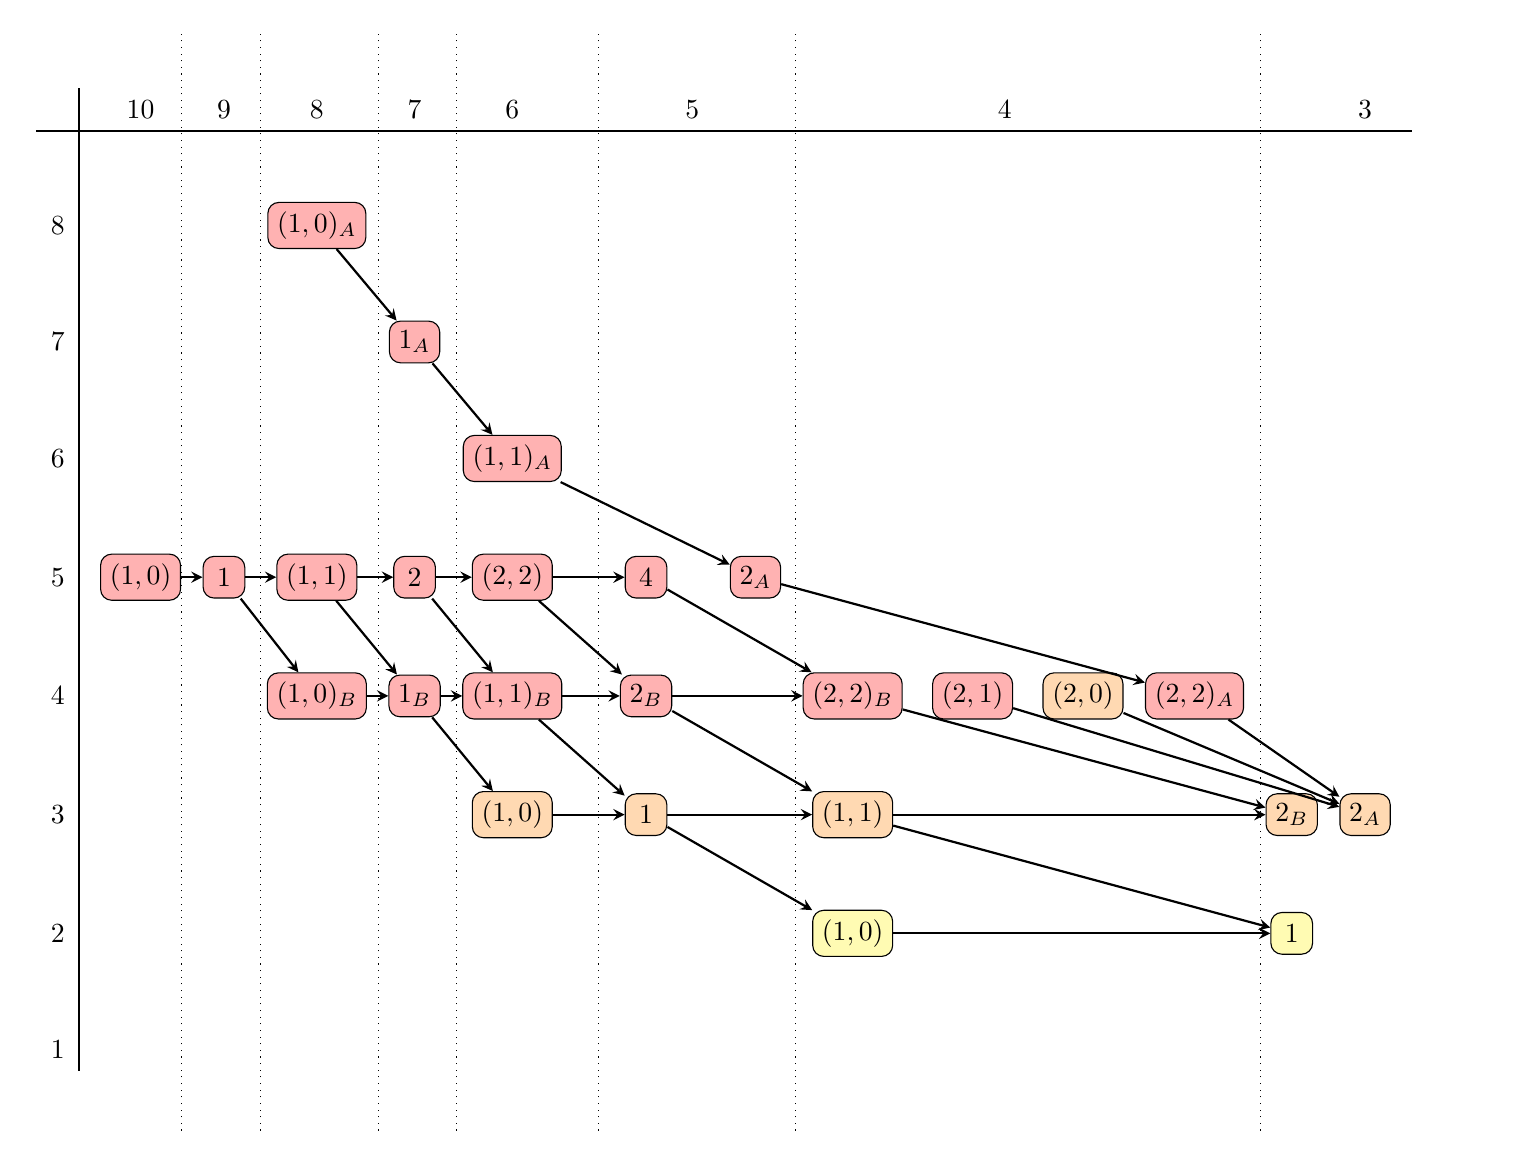
\begin{tikzpicture}
  \matrix (mat) [nodes in empty cells, minimum width=3.5ex, minimum height=3.5ex, column sep=1.8ex,row sep=6ex]{
   \node (corner) {}; & \node (d10) {10}; & \node (d9) {9}; & \node (d8) {8}; & \node (d7) {7}; & \node (d6) {6}; & \node {$\qquad \quad \ 5$}; && \node (d5) {};& \node {$\qquad \ 4$}; && \node (d4) {}; & &\node (d3) {3}; & \node (d2) {}; &  \\
  \node {8}; &    &   & \node[s16] (88) {$(1,0)_A$};  &   &   &   &&   &&&&   &&&   \\
  \node {7}; &    &   &   & \node[s16] (77) {$1_A$};  &   &   &&   &&&&   &&&   \\
  \node {6}; &    &   &   &   & \node[s16] (66) {$(1,1)_A$};  &   &&   &&&&   &&&   \\
  \node {5}; & \node[s16] (105) {$(1,0)$};  & \node[s16] (95) {$1$};  & \node[s16] (85) {$(1,1)$};  & \node[s16] (75) {$2$}; & \node[s16]  (65){$(2,2)$};  & \node[s16] (55B) {$4$}; & \node[s16] (55A) {$2_A$};  &   &&&&   &&&   \\
  \node {4}; &    &   & \node[s16] (84) {$(1,0)_B$};  & \node[s16] (74) {$1_B$};  & \node[s16] (64) {$(1,1)_B$};  & \node[s16] (54) {$2_B$};  && \node[s16] (44B) {$(2,2)_B$}; & \node[s16] (44K) {$(2,1)$}; & \node[s8] (44A) {$(2,0)$}; & \node[s16] (44g) {$(2,2)_A$};  &   &&&   \\
  \node {3}; &    &   &   &   & \node[s8] (63) {$(1,0)$};  & \node[s8] (53) {$1$};  && \node[s8] (43) {$(1,1)$};  &&&& \node[s8] (33B) {$2_B$}; & \node[s8] (33A) {$2_A$}; &  &   \\
  \node {2}; &    &   &   &   &   &   && \node[s4](42) {$(1,0)$};  &&&& \node[s4] (32) {$1$};  &&   \\
  \node (i1) {1}; &   &  &  &  &  &   & &   &&& &   && &   \\};
  
  \draw[thick] (corner.south west) -- (d2.south west);
  \draw[thick] (corner.north east) -- (i1.south east);
  
  \draw[dotted] (0.5,-7) -- (0.5,7);
  \draw[dotted] (6.4,-7) -- (6.4,7);
  \draw[dotted] (-2,-7) -- (-2,7);
  \draw[dotted] (-3.8,-7) -- (-3.8,7);
  \draw[dotted] (-4.8,-7) -- (-4.8,7);
  \draw[dotted] (-6.3,-7) -- (-6.3,7);
  \draw[dotted] (-7.3,-7) -- (-7.3,7);
  
  \draw[arrow] (105) -- (95);
  \draw[arrow] (95) -- (85);
  \draw[arrow] (88) -- (77);
  \draw[arrow] (95) -- (84);
  \draw[arrow] (85) -- (75);
  \draw[arrow] (85) -- (74);
  \draw[arrow] (84) -- (74);
  \draw[arrow] (77) -- (66);
  \draw[arrow] (75) -- (65);
  \draw[arrow] (75) -- (64);
  \draw[arrow] (74) -- (64);
  \draw[arrow] (74) -- (63);
  \draw[arrow] (66) -- (55A);
  \draw[arrow] (65) -- (55B);
  \draw[arrow] (65) -- (54);
  \draw[arrow] (64) -- (54);
  \draw[arrow] (64) -- (53);
  \draw[arrow] (63) -- (53);
  \draw[arrow] (55A) -- (44g);
  \draw[arrow] (55B) -- (44B);
  \draw[arrow] (54) -- (44B);
  \draw[arrow] (54) -- (43);
  \draw[arrow] (53) -- (43);
  \draw[arrow] (53) -- (42);
  \draw[arrow] (44B) -- (33B);
  \draw[arrow] (44A) -- (33A);
  \draw[arrow] (44K) -- (33A);
  \draw[arrow] (43) -- (33B);
  \draw[arrow] (43) -- (32);
  \draw[arrow] (42) -- (32);
  \draw[arrow] (44g) -- (33A);
  
\end{tikzpicture}
\caption{This figure shows the orbits of square-zero supercharges in each dimension.  The labels indicate each orbit: the number refers to the rank, and the subscript indicates the situations where the supercharges of a given rank split into multiplet orbits.  Each column is labelled by a dimension, and each row by the number of invariant directions of the supercharge.  Colours indicate the maximal supersymmetry algebra where the given supercharges live, so red indicates supercharges defined in algebras with 16 supercharges, orange those with 8 supercharges, and yellow those with 4 supercharges.}
\label{fig:superchargeorbits}
\end{figure}

\subsection*{Outline of the Paper}
%\addcontentsline{toc}{subsection}{Outline of the Paper}
The remainder of the paper is divided into two parts.  In Part \ref{formalism_part} we set up the formalism that we will use when we study supersymmetric gauge theories and their twists.  The first main ingredient is the Batalin-Vilkovisky formalism \cite{BatalinVilkovisky} for classical field theory (Section \ref{BV_section}), as developed by Costello and Gwilliam in \cite{CostelloBook, Book1, Book2}.  The other main ingredient is the systematic study of supersymmetry algebras and supersymmetric action functionals using normed division algebras (Section \ref{sect:susy}), following Baez and Huerta \cite{BaezHuerta}.  We use this formalism to prove in Section \ref{sect:SYM} that super Yang-Mills theories with matter in dimensions 10, 6, 4 and 3 are in fact supersymmetric, meaning that there is a well-defined $L_\infty$ action of the supersymmetry algebra on the classical BV theory in question.  We introduce the idea of dimensional reduction (Section \ref{dim_red_section}) for classical field theories to show that supersymmetry action are well-defined in lower dimensions.

In Part \ref{classification_part} of the paper, we produce the classification of supersymmetric Yang-Mills theories in dimensions 2 to 10 systematically.  We start with dimension 10 and work down by dimensional reduction.  Each subsection is divided by the number of supersymmetries, and the orbits of square-zero supercharges by which we can twist.  Twisted theories are characterized up to perturbative equivalence, including the residual Lorentz symmetry acting on each twisted theory.

\subsection*{Acknowledgements}
We would like to thank Owen Gwilliam, Justin Hilburn and Philsang Yoo for helpful discussions during the preparation of this paper.  We are also grateful to Dylan Butson for kind discussion of his related forthcoming work.  The research of CE on this project has received funding from the European Research Council (ERC) under the European Union's Horizon 2020 research and innovation programme (QUASIFT grant agreement 677368).

\part{Supersymmetric Gauge Theory} \label{formalism_part}

\section{The BV-BRST Formalism} \label{BV_section}

In this section we will set up the homological formalism in which we study classical field theory: the BV-BRST formalism.  Most of the material in this section is not original.  We refer the reader to \cite{CostelloBook, Book2} for more details on this perspective.  We will conclude the section by describing a number of fundamental examples of classical field theories that are highly structured: partially holomorphic or topological theories.  We will also discuss the concept of \emph{dimensional reduction} of a classical field theory on $M$ along a fibration $M \to N$.  We will use the idea of dimensional reduction to construct many of the supersymmetric field theories which we will consider in the next section.  

\subsection{Conventions}
Throughout the paper we will frequently study obects, for instance vector bundles, equipped with a $\ZZ\times\ZZ/2\ZZ$-grading. \emph{Degree} will refer to the first (cohomological) grading and \emph{odd} or \emph{even} to the second (fermionic) grading.  For an element $x$ we denote by $|x|\in\ZZ/2\ZZ$ the total degree.

Given a vector bundle $E\rightarrow M$ we denote by $\cE$ the topological vector space of smooth sections of $E$ and $\cE_c$ the topological vector space of smooth compactly supported sections.
We denote by $\cO(\cE)$ (respectively $\cO(\cE_c)$) the completed algebra of symmetric functions on $\cE$ (respectively $\cE_c)$. 
We denote by $\oloc(\cE)$ the space of local functionals on $\cE$ (see \cite[Definition 4.5.1.1]{Book2}). An element of $\oloc(\cE)$ will be denoted symbolically by an expression of the form
\[\int_M f (\phi, \phi', \dots),\]
where $f$ is a density on $M$ depending on infinite jets of sections of $E$. Note, however, that the integral here is a formal symbol. 
The space of local functionals can be viewed as a subspace
\[
\oloc(\cE) \subset \cO(\cE_c)
\]
where the integral symbol makes sense in earnest when applied to sections which are compactly supported.
We denote by $\oloc^+(\cE)\subset \oloc(\cE)$ the subspace of local functionals which are at least cubic.

Given two vector bundles $E, F$ on $M$ we can also make sense of the space of local functionals from $E$ to $F$.
By definition, this is 
\[
{\rm Fun}_{\rm loc}(\cE, \cF) = \prod_{n \geq 0} {\rm PolyDiff}(\cE^{\times n}, \cF)_{S_n}
\]
where ${\rm PolyDiff}(\cE^{\times n}, \cF)$ denotes the space of polydifferential operators, and we take coinvariants for the obvious symmetric group action.
When $\cF = \cE$, we refer to ${\rm Fun}_{\rm loc}(\cE, \cE)$ as the space of local vector fields on $E$. 
There is a natural Lie bracket on ${\rm Fun}_{\rm loc}(\cE, \cE)$ and a canonical action of this Lie algebra on local functionals. 

\subsection{Local formal moduli problems}


\subsection{Classical BV Theories}

The classical BV (Batalin-Vilkovisky) formalism \cite{BatalinVilkovisky} is a model for classical field theory from the Lagrangian perspective.  In brief the classical BV formalism produces a local model for the critical locus of an action functional, but considered in the derived sense.  That is, given a space $\Phi$ of fields and an action functional with derivative $\d S$, one considers not just the usual locus in $\Phi$ of fields with $\d S(\phi) = 0$, but the derived intersection $\mr{dCrit}(S) = \Phi \cap^h_{T^*\Phi} \Gamma_{\d S}$ of the zero section in $T^*\Phi$ with the graph of $\d S$.  The formalism we describe below can be interpreted as an abstract formalism for modelling the tangent complex at a point to a derived critical locus $\mr{dCrit}(S)$.

\begin{definition}
A \defterm{free BV theory} on a manifold $M$ is the data of:
\begin{itemize}
\item a finite rank $\ZZ\times\ZZ/2\ZZ$-graded vector bundle $E \to M$ equipped with an even differential operator of cohomological degree $+1$
\[
Q_{\mr{BV}} \colon \cE \to \cE [1] 
\]
such that $(1)$: $Q_{\mr{BV}}^2 = 0$ and $(2)$: the pair $(\cE , Q_{\mr{BV}})$ is an elliptic complex;
\item a map of bundles
\[
\omega\colon E \otimes E \to \Dens_M [-1]
\]
that is
\begin{enumerate}
\item[$(1)$] fiberwise nondegenerate,
\item[$(2)$] graded skew symmetric, and
\item[$(3)$] satisfies $\int_M \omega(e_0, Q_{\mr{BV}} e_1) = (-1)^{|e_0|} \int_M \omega(Q_{\mr{BV}} e_0, e_1)$ where $e_i$ are compactly supported sections of $E$ .
\end{enumerate}
\end{itemize}
\end{definition}

We call $\cE$ the \defterm{space of BV fields}. The pairing $\omega$ equips the algebra of local functionals on $E$ with a \defterm{BV bracket} (see \cite[Chapter 5.3]{CostelloBook}) 
\[
\{-,-\}\colon \oloc(\cE) \times \oloc(\cE) \to \oloc(\cE) .
\]
This bracket is of cohomological degree $+1$. 
This bracket is a graded version to the so-called Soloviev bracket defined on the $\infty$-jets, as described in Section 4 of \cite{GetzlerBracket}. 

We explain how to define the BV bracket in our context.  
First note that there is a linear map
\[
\d_{\mr{dR}} \colon \oloc(\cE) \to {\rm Fun}_{\rm loc}(\cE, \cE^!) 
\]
defined as follows. 
A local functional $F \in  \oloc(\cE)$ can be written as an equivalence class of a sum of densities of the form
\[
D_1(-) \cdots D_n(-) \Omega
\]
where $D_i$ is a differential operator $D_i \colon \cE \to C^\infty_M$ and $\Omega$ is a density on $M$. 
Without loss of generality, suppose $F$ is of this form. 
Then, we can view $F$ as a functional in $\cO(\cE_c)$ by the assignment
\[
\phi \mapsto \int_M D_1(\phi) \cdots D_n(\phi) \Omega
\]
where $\phi$ denotes a compactly supported section. 
Define the symmetric multilinear map
\[
\begin{array}{ccccl}
\d_{\mr{dR}} F & \colon & \cE_c^{\times (n-1)} & \to & \cE^\vee \\
& & (\phi_1, \ldots, \phi_{n-1}) & \mapsto & D_1(\phi_1) \cdots D_{n-1}(\phi_{n-1}) D_{n} (-) + \{{\rm symmetric\;terms}\} .
\end{array}
\]
Integrating by parts, we see that for any $(n-1)$-tuple $\phi_1, \ldots, \phi_{n-1} \in \cE_c$ that the linear functional $(\d_{\mr{dR}} F) (\phi_1,\ldots, \phi_{n-1})$ is an element of $\cE^!$. 
This implies that $\d_{\mr{dR}} F \in {\rm Fun}_{\rm loc}(\cE, \cE^!)$.

The non-degenerate pairing $\omega$ determines a bundle isomorphism $\omega \colon E \cong E^! [-1]$ and hence an isomorphism of local functions
\[
\omega \colon {\rm Fun}_{\rm loc}(\cE, \cE^!) \cong {\rm Fun}_{\rm loc}(\cE, \cE[1]) .
\]
We recognize the right hand side as the space of local vector fields placed in a shifted cohomological degree.
In total, we see that a local functional $F$ determines a local vector field by applying this isomorphism to $\d_{\mr{dR}}F$:
\[
X_F := \omega \circ \d_{\mr{dR}} (F) \in  {\rm Fun}_{\rm loc}(\cE, \cE[1])  .
\]
This is the Hamiltonian vector field corresponding to $F$. 
Finally, the BV bracket between local functionals $F, G$ is defined by
\[
\{F, G\} = X_F (G) .
\]

The BV bracket enjoys the graded skew symmetry property
\[
\{F, G\} = (-1)^{|F| |G|} \{G, F\}
\]
as well as the graded Jacobi identity.
This bracket together wtih $Q_{\mr{BV}}$ endows $\oloc(\cE)[-1]$ with the structure of a dg Lie algebra. 
Since the space of local functionals is not an algebra, the bracket does not satisfy any type of Leibniz rule. 

%\[
%\{F(A, B), G(A, B)\} = \frac{\partial}{\partial A} F(A, B) \frac{\partial}{\partial B}  G(A,B) + \frac{\partial}{\partial B} F(A, B) \frac{\partial}{\partial A}  G(A,B)
%\]

Now, we will include interactions in the BV picture. 

\begin{definition}
A \defterm{classical BV field theory} (or simply, classical field theory) is a free BV theory $(E, Q, \omega)$ equipped with an even functional
\[I \in \oloc^+(\cE)\]
of cohomological degree zero satisfying the Maurer-Cartan equation
\[Q_{\mr{BV}} I + \frac{1}{2} \{I,I\} = 0 .\]
\label{def:classicalfieldtheory}
\end{definition}

Given a classical field theory $(E, Q_{\mr{BV}}, \omega, I)$ we denote by
\[S = \frac{1}{2} \int_M \omega(e, Q_{\mr{BV}} e) + I\in \oloc(E)\]
the BV action of the theory.

The local functional $S$ satisfies the {\em classical master equation} \[\{S, S\} = 0.\] 

In fact, given a degree $(-1)$ nondegenerate pairing $\omega$ on $E$, prescribing the data of a classical field theory (namely a pair $Q_{\mr{BV}}, I$ satisfying the Maurer-Cartan equation) is equivalent to prescribing a local functional $S \in \oloc(\cE)$ that is at least quadratic and satisfies the classical master equation.
The operator $Q_{\mr{BV}}$ is the BV bracket with the quadratic part of the BV action $S$, and the cubic and higher terms in $S$ coincide with $I$.

Because of this, we will sometimes refer to the triple $(E, S, \omega)$ instead $(E, Q_{\mr{BV}}, I, \omega)$ as the data of a classical field theory.

\begin{remark}
We will also consider \defterm{$\ZZ/2\ZZ$-graded classical field theories} which are defined as before, but where $E$ has only a single $\ZZ/2\ZZ$-grading and, correspondingly, $Q_{\mr{BV}}$ is simply an odd operator.
\end{remark}

\begin{remark}
The data of a classical BV theory can be equivalently encoded in an elliptic $L_\infty$ algebra $L=E[-1]$ equipped with a cyclic structure, i.e. a symplectic isomorphism $L\cong L^![-3]$ \cite[Chapter 5.4]{Book2}. 
\end{remark}

We will also sometimes consider $\CC[t]$-families of classical field theories.  These will be defined as follows.
\begin{definition} \label{family_of_BV_theories_def}
A $\CC[t]$-family of classical BV theories is a quadruple $(E,Q_{\mr{BV}}, \omega, I)$ as before, but where now the classical BV differential is $t$-dependent.  In other words, it is given as a map
\[Q_{\mr{BV}} \colon \cE \to \cE  \otimes \CC[t] [1],\]
where, for each $t_0 \in \CC$, the quadruple $(E,Q^{t_0}_{\mr{BV}}, \omega, I)$
\[Q^{t_0}_{\mr{BV}} = \mr{ev}_{t_0} \circ Q_{\mr{BV}} \colon \cE \to \cE  \otimes \CC[t] [1] \to \cE[1]\]
defines a classical field theory.
\end{definition}

Next, we formulate the notion of an equivalence of classical BV theories. 

\begin{definition}
A \defterm{morphism} $\Phi \colon (E, Q_{\mr{BV}}, \omega, I) \rightsquigarrow (E', Q_{\mr{BV}}', \omega', I')$ of classical field theories over the same manifold $M$ is
% a nonlinear map of vector bundles $E\rightsquigarrow E'$, 
a collection $\Phi =\sum_{n\geq 1}^\infty \Phi_n$ of poly-differential operators $\Phi_n\colon \Sym^n(E)\rightarrow E'$, that intertwines the differentials $Q_{\mr{BV}}, Q_{\mr{BV}}'$, the pairings $\omega, \omega'$, and the interactions $I,I'$. A morphism is a \defterm{perturbative equivalence} if the map $\Phi_1\colon (\cE, Q_{\mr{BV}})\rightarrow (\cE', Q_{\mr{BV}}')$ is a quasi-isomorphism. 
A classical field theory is \defterm{perturbatively trivial} if it is perturbatively equivalent to the zero theory ($E = 0$).
\label{def:perturbativeequivalence}
\end{definition}

We will now describe two primitive examples of equivalences of classical field theories which will be useful in simplifying twisted theories. 
First, we consider the process of integrating out an auxiliary field.

\begin{prop}\label{prop:integrateoutfield}
Fix a volume form $\dvol_M$ on $M$. Suppose $(E, \omega, S)$ is a classical field theory, where $E\cong E_0\oplus (\cO_M\oplus \Dens_M[-1])$ with the symplectic pairing $\omega$ given by a sum of a symplectic pairing $\omega_0$ on $E_0$ and the standard symplectic pairing on the second summand. Denote by $\phi$ a section of $\cO_M$ and by $\phi^*$ a section of $\Dens_M[-1]$. Suppose the BV action is
\[S = S_0 + \frac{1}{2} \int \dvol_M (\phi^2 - 2\phi S_1),\]
where $S_0$ is a local functional independent of $\phi,\phi^*$ and $S_1$ is a $\cO_M$-valued polydifferential operator which is independent of $\phi$. 
Then the theory $(E, Q, \omega, I)$ is perturbatively equivalent to the theory $(E_0, \omega_0, S')$ with the BV action $S' = S_0 - S_1^2/2$, where we set and $\phi = S_1$ and $\phi^* = 0$.
\end{prop}

\begin{remark}
In terms of the classical BV complex, this proposition tells us that if a classical BV complex is of the form
\[\xymatrix{
\cdots & \ul{0} & \ul{1} & \cdots \\
\cdots \ar[r] & E_0^0 \ar[r]^{Q_0} \ar[dr] & E_0^1 \ar[r] &\cdots \\
&\cO_M \ar^{{\rm dvol}}[r] \ar[ur] &\dens_M &
}\]
where the bottom map multiplies a function by the volume element, then we can replace it with a quasi-isomorphic cochain complex consisting of only the first line, provided we make a suitable modification of the classical action functional. 
\end{remark}

\begin{proof}
Concretely, suppose that the linear part of $S_1$ is given by an operator $Q_1$, and the interacting part of $S_1$ is given by a functional $I_1 = \sum_{n=1}^\infty I_1^n$.  
The desired equivalence $\Phi \colon (E, \omega, S) \to (E_0, \omega_0, S')$ is given by the natural projection $\Phi = \Phi_1 \colon E \to E_0$. 
The quasi-inverse $\Psi \colon (E_0, \omega_0, S') \to (E, \omega, S)$ is defined as follows.
First $\Psi_1(e) = (e, Q_1(e), 0) \in E$.
For $n > 1$, define
\begin{align*}
\Psi_n \colon \sym^n(E_0) &\to E \\
e_1 \otimes \cdots \otimes e_n &\mapsto (0, I_1^n(e_1, \ldots, e_n), 0).
\end{align*}
These $\Psi_n$ manifestly intertwines the pairings $\omega$ and $\omega'$.  
To see that they intertwine the action functionals, we observe that 
\begin{align*}
S(\Psi(e)) &= S(e, S_1(e), 0) \\
&= S_0(e) + \frac 12 \dvol_M \int (S_1(e)^2 - 2 S_1(e)^2) \\
&= S_0(e) - \frac 12 S_1(e)^2 \\
&= S'(e).
\end{align*}
\end{proof}

We may also remove a trivial BRST doublet.

% \begin{prop}
% Suppose $(E, Q_{\mr{BV}}, \omega, I)$ is a classical field theory, $F\rightarrow M$ is a graded vector bundle, such that $E\cong E_0\oplus E_1\oplus E_1^![-1]\oplus E_1^!\oplus E_1[-1]$. Denote by $\phi, \phi^*$ sections of $E_1,E_1^![-1]$ and by $\psi, \psi^*$ sections of $E_1^!, E_1[-1]$. Suppose
% \[Q_{\mr{BV}}\phi + \{I, \phi\} = \phi - f_\psi \in E_1[-1] ,\qquad Q\psi + \{I, \psi\} = \psi - f_{\phi} \in E_1^![-1],\]
% where $f_\phi$ is independent of $\psi$ and $f_{\psi}$ is independent of $\phi$. Then the theory $(E, Q_{\mr{BV}}, \omega, I)$ is perturbatively equivalent to the theory $(E_0, Q_0, \omega_0, I_0)$ with the BV action obtained by setting $\phi = f_\psi, \phi^* = 0,  \psi = f_\phi, \psi^* = 0$ in the original BV action.
% \end{prop}

\begin{prop} 
\label{prop:BRSTdoublet}
Let $(E_0, \omega_0, S_0)$ be a classical BV theory and $F \to M$ a graded vector bundle.
Consider the theory $(E, \omega, S)$ with underlying graded vector bundle
\[
E = E_0 \oplus \left(F \oplus F^! [-1]\right) \oplus \left(F^! \oplus F[-1] \right)
\]
whose sections we denote by $e_0 + \varsigma + \varsigma^* + \psi + \psi^*$ according to the above decomposition. 
The shifted symplectic form $\omega$ is given by the sum of $\omega_0$ plus the standard degree $+1$ pairings between $F, F^! [-1]$ and $F^!, F[-1]$. 
Suppose further that the local functional
\[
S = S_0 + \int \phi \psi^* - \int \phi I_\phi - \int \psi^* I_{\psi^*} - \int \phi^* I_{\phi^*} - \int \psi I_{\psi}
\]
satisfies the classical master equation, where $I_{\phi}, I_{\psi^*}, I_{\phi^*}, I_{\psi}$ are polydifferential operators on fields valued in $F^!$, $F$, $F$, $F^!$ respectively, and which are independent of $\phi$ and $\psi^*$.
Then, the classical BV theory $(E, \omega, S)$ is perturbatively equivalent to the BV theory $(E_0, \omega_0, S')$ where $S'$ is given by setting $\phi = I_{\psi^*}, \phi^* = 0$ and $\psi^* = I_{\phi}, \psi = 0$ in the original action functional $S$. 
\end{prop}

\begin{remark}
For the classical BV theory $(E, \omega, S)$ as in the proposition, the linearized BV differential defines the following cochain complex of fields:
%\[\xymatrix{
%\cdots & \ul{-1} & \ul{0} & \ul{1} & \ul{2} & \cdots \\
%\cdots \ar[r] & E_0^{-1}\ar[r] \ar[dr] \ar[ddr] &E_0^0 \ar[r]  &E_0^1 \ar[r] &E_0^2 \ar[r] &\cdots \\
%&&F_\phi \ar^{~}[dr] &F^!_{\phi*} \ar[ur] && \\
%&&F^!_{\psi^*} \ar^{~}[ur] &F_\psi \ar[uur] && \\
%}\]
\[\xymatrix{
\cdots & \ul{-1} & \ul{0} & \ul{1} & \ul{2} & \cdots \\
\cdots \ar[r] & E_0^{-1}\ar[r] \ar@{.>}[dr] \ar@{.>}[ddr] &E_0^0 \ar@{.>}[ddr] \ar@{.>}[dr]  \ar[r]  &E_0^1 \ar[r] &E_0^2 \ar[r] &\cdots \\
&&F_\phi \ar^{~}[dr]  \ar@{.>}[ur] &F^!_{\phi*}  \ar@{.>}[ur] && \\
&&F^!_{\psi^*} \ar^{~}[ur]  \ar@{.>}[uur]  &F_\psi  \ar@{.>}[uur] && \\
}\]
where the subscripts match the notation for the fields in the statement above. \footnote{Note that we are writing $F$ as if it is concentrated in a single cohomological degree, but the proposition applies for any graded vector bundle as in the statement of the proposition.}
The top line is the underlying cochain complex of the theory with fields $E_0$. 
The arrows $F_\phi \to F_\psi$ and $F^!_{\psi^*} \to F^!_{\phi^*}$ are given by the identity.
The dotted arrows represent terms in the differential arising from $I_\phi, I_{\psi^*}, I_{\phi^*}, I_{\psi}$. 
The above proposition implies we can replace this cochain complex of fields with a quasi-isomorphic complex consisting of only the first line, provided we make a suitable modification of the classical action functional. 
\end{remark}

\begin{proof}
Concretely, we'll write $\sum_{n \ge 1} I^{(n)}_\phi$ and $\sum_{n \ge 1} I^{(n)}_{\psi^*}$ for the Taylor expansions of $I_\phi$ and $I_{\psi^*}$ respectively.  
The desired equivalence $\Phi \colon (E, \omega, S) \to (E_0, \omega_0, S')$ is given by the natural projection $\Phi = \Phi_1 \colon E \to E_0$. 
The quasi-inverse $\Psi \colon (E_0, \omega_0, S') \to (E, \omega, S)$ is defined as follows.
The linear term is $\Psi_1(e) = (e, I^{(1)}_{\phi}(e),0,0, I^{(1)}_{\psi^*}(e))$, and for $n > 1$ we have 
\[\Psi_n(e_1\otimes \cdots \otimes e_n) = (0, I^{(n)}_{\phi}(e_1, \ldots, e_n), 0, I^{(n)}_{\psi^*}(e_1, \ldots, e_n)).\]

The maps $\Psi_n$ manifestly intertwine the pairings on $E_0$ and $E$, since the image of $\Psi_n$ lands in an isotropic summand of the $E_1\oplus E_1^![-1]\oplus E_1^!\oplus E_1[-1]$ part of $E$.  
Also, by construction, the $\Psi_n$ intertwine the action functionals, since
\begin{align*}
S(F(e)) &= S_0(e) + \frac{1}{2} \int_M \omega(I_{\psi^*}(e), I_\phi(e) - I_\phi(e)) + \omega(I_\phi (e), I_{\psi^*}(e) - I_{\psi^*}(e)) \\
&= S'(e).
\end{align*}
\end{proof}

%There is a corollary of this proposition obtained by iterating the procedure. 
%We will only use a single iteration. 
%
%\begin{cor} \label{cor: quad}
%Let $(E_0, \omega_0, S_0)$ be a classical BV theory and $F \to M$ a graded vector bundle.
%Consider the theory $(E, \omega, S)$ with underlying graded vector bundle
%\[
%E = E_0 \oplus \bigoplus_{i=1}^2 \left(F \oplus F^! [-1]\right) \oplus \bigoplus_{i=1}^2 \left(F^!  \oplus F[-1] \right)
%\]
%whose sections we denote by $e_0 + \sum_{i=1}^2 (\phi + \phi_i^*) + \sum_{i=1}^2(\psi_i + \psi_i^*)$ according to the above decomposition. 
%The shifted symplectic form $\omega$ is given by the sum of $\omega_0$ plus the standard degree $+1$ pairings between $F, F^! [-1]$ and $F^!, F[-1]$.
%Suppose further that the local functional
%\[
%S = S_0 + \int \left(\phi_2\psi^*_1 + (\phi_2 - \phi_1)\psi_2^*\right) -  \sum_{i=1}^2 \int \phi_i I_{\phi,i} - \sum_{i=1}^2 \int \psi_i^* I_{\psi^*,i} -  \sum_{i=1}^2 \int \phi^*_i I_{\phi^*,i} - \sum_{i=1}^2 \int \psi_i I_{\psi,i} 
%\]
%satisfies the classical master equation, where $I_{\phi,i}, I_{\psi^*,i}, I_{\phi^*,i}, I_{\psi,i}$ are polydifferential operators on fields valued in $F^!$, $F$, $F$, $F^!$ respectively, and which are independent of the fields $\phi_i$ and $\psi^*_i$.
%Then, the classical BV theory $(E, \omega, S)$ is perturbatively equivalent to the BV theory $(E', \omega_0, S')$ where 
%\[
%E' = E_0 \oplus \left(F_{\phi_1} \oplus F^!_{\phi_1^*} [-1]\right) \oplus \left(F^!_{\psi_1^*} \oplus F[-1]_{\psi_1} \right)
%\]
%and
%\[
%S' = S_0 + \int \phi_1 \psi_1^* - S''
%\]
%where $S'$ is given by setting $\phi = I_{\psi^*}, \phi^* = 0$ and $\psi^* = I_{\phi}, \psi = 0$ in the functional functional $S$.\brian{finish}
%\end{cor}
%\begin{proof}
%%Notice that the collection of fields $(e_0, \phi_1, \phi_1^*, \phi_2, \phi_2^*, \psi_1, \psi_1^*, \psi_2, \psi_2^*)$ have the same shifted Poisson brackets as the collection of fields $(\phi_1, \phi_1^*
%We begin by making the following change of coordinates on the BV fields:
%\begin{align*}
%\Tilde{\phi}_2 & = \phi_2 - \phi_1 \\
%\Tilde{\psi}_2 & = \psi_2 + \psi_1 \\
%%\Tilde{\phi}^*_2 & = \phi^*_2 - \phi^*_1 \\
%%\Tilde{\psi}^*_2 & = \psi^*_2 + \psi^*_1 
%\end{align*}
%with $\phi_1, \psi_1$ left fixed. 
%This change of coordinates is compatible with the $(-1)$-symplectic pairing. 
%Further, in the new coordinates, the action takes the form
%\[
%S = S_0 + \int \Tilde{\phi}_2\Tilde{\psi}^*_2 + \int \phi_1\psi_2^* -  \sum_{i=1}^2 \int \phi_i I_{\phi,i} - \sum_{i=1}^2 \int \psi_i^* I_{\psi^*,i} 
%\]
%\end{proof} 

\subsection{Symmetries in the Classical BV Formalism} \label{symmetry_section}
In this section we define what it means for a (super) Lie algebra to act on a classical field theory  (see also \cite[Chapter 11]{Book2} for a related discussion). Let $(E, Q_{\mr{BV}},\omega, I)$ be a classical field theory and $\fg$ a super Lie algebra.  We will define $\gg$-equivariant local observables in the classical field theory by introducing $\gg$-valued background fields into our classical field theory, and extending the action functional to a functional that involves these background fields, but still satisfies the classical master equation.  We begin by defining an appropriate version of the Chevalley-Eilenberg cochain complex.

\begin{definition}
The \emph{Chevalley-Eilenberg complex} for the Lie algebra $\gg$, with coefficients in $\oloc(\cE)$, will be defined as follows.  Consider the graded vector space
\[C^\bullet(\fg, \oloc(\cE)) = \bigoplus_n \hom(\wedge^n \fg, \oloc(\cE))[-n]\]
parametrizing multilinear maps $f\colon \fg^{\otimes n}\rightarrow \oloc(\cE)$ which satisfy the antisymmetry property
\[f(x_1, \dots, x_i, x_{i+1}, \dots, x_n) = (-1)^{|x_1||x_2|+1} f(x_1, \dots, x_{i+1}, x_i, \dots, x_n)\]
where $x_j \in \fg$.  The Chevalley-Eilenberg differential is given, following the sign conventions of \cite{SafronovCoisoInt}, by the formula
\[(\d_{\mr{CE}} f)(x_1, \dots, x_n) = \sum_{i < j}(-1)^{|x_i| \sum_{p=1}^{i-1} |x_p| + |x_j| \sum_{p=1,p\neq i}^{j-1} |x_p| +i+j+|f|} f([x_i, x_j], x_1, \dots, \widehat{x}_i, \dots, \widehat{x}_j, \dots, x_n).\]
The complex is additionally equipped with a degree $+1$ BV bracket via the formula
\[\{f, g\}(x_1, \dots, x_{k+l}) = \sum_{\sigma\in S_{k, l}} \mathrm{sgn}(\sigma) (-1)^{\epsilon+\epsilon_1} \{f(x_{\sigma(1)}, \dots, x_{\sigma(k)}), g(x_{\sigma(k+1)}, \dots, x_{\sigma(k+l)})\},\]
where $S_{k, l}$ is the set of $(k, l)$-shuffles, $\epsilon$ is the usual Koszul sign and
\[\epsilon_1 = |g|k + \sum_{i=1}^k |x_{\sigma(i)}|(l+|g|).\]
\end{definition}

The operator $Q_{\mr{BV}}$ on $\oloc(\cE)$ extends $C^\bu(\fg)$-linearly to an operator on $C^\bullet(\fg, \oloc(\cE))$ by the rule
\[
(Q_{\mr{BV}} f)(x_1,\ldots, x_n) = Q_{\mr{BV}} f(x_1,\ldots, x_n) 
\]
where $f \colon \fg^{\otimes n} \to \oloc(\cE)$. 
The differentials $\d_{\mr{CE}}$ and $Q_{\mr{BV}}$ are compatible in the sense that $(\d_{\mr{CE}} + Q_{\mr{BV}})^2 = 0$ making $C^\bu(\fg, \oloc(\cE))$ into a cochain complex with total differential $\d_{\mr{CE}} + Q_{\mr{BV}}$. 
Via the BV bracket, the shift of this cochain complex $C^\bu(\fg, \oloc(\cE))[-1]$ is a dg Lie algebra.  This shifted cotangent complex will model equivariant local observables in our classical field theory, but to finish defining the $\gg$ action we must define the equivariant version of the classical interaction.  This is defined as follows.

\begin{definition}
\label{infinitesimal_action_def}
Let $(E, Q_{\mr{BV}},\omega, I)$ be a classical field theory. 
%\begin{itemize}
%\item[(1)]
An \defterm{action} of a super Lie algebra $\fg$ on $(E, Q_{\mr{BV}}, \omega, I)$ is an element of cohomological degree zero 
\[I_\fg = \sum_{k\geq 0} I_{\fg}^{(k)} \text{ in } C^\bullet(\fg, \oloc(\cE)),\]
where $I_\fg^{(k)}$ is a multilinear map $\fg^{\otimes k} \to \oloc(\cE)$, that satisfies the following three conditions:
\begin{itemize}
\item[(a)] $I_\fg^{(0)} = I$.
\item[(b)] For each $k \geq 1$ and $x_1, \ldots, x_k \in \fg$ the local functional $I^{(k)}_\fg (x_1,\ldots, x_k)$ is at least quadratic in the fields.
\item[(c)] $I_\fg$ satisfies the Maurer--Cartan equation:
\[(\d_{\mr{CE}} + Q_{\mr{BV}}) I_\fg + \frac{1}{2} \{I_\fg, I_\fg\} = 0.\]
\end{itemize}
%\item[(2)]
%For each $k \geq 1$ there is a decomposition $I_\fg^{(k)} = \sum_{\ell} I_\fg^{(k),\ell}$ where $ I_\fg^{(k),\ell}(x_1,\ldots,x_k) \in \oloc(\cE)$ is $\ell$-linear in the fields $\cE$ for all $x_1,\ldots,x_k \in \fg$.
%An action $I_\fg$ is called \defterm{elliptic} if the induced linear differential operator
%\[
%Q_{\mr{BV}} + \sum_{k \geq 1} \{I_\fg^{(k),2}, -\}
%\]
%is elliptic as a $C^\bu(\fg)$-linear differential operator.
%\end{itemize}
\end{definition}

\begin{remark}
We have seen that a classical BV theory can also be presented in terms of a BV action $S \in \oloc(\cE)$ satisfying the classical master equation $\{S, S\} = 0$. 
One can also formulate actions of a Lie algebra on a classical theory in these terms. 
The data of an action of a Lie algebra $\fg$ on a classical field theory $(E, \omega, S)$ is equivalent to the choice of a local functional $\fS_\fg = \sum_k \fS_\fg^{(k)}\in C^\bu(\fg, \oloc(\cE))$, at least quadratic in the fields, such that $\fS^{(0)}_\fg = S$ and such that the classical master equation
\[
\d_{\mr{CE}} \fS_\fg + \frac{1}{2} \{\fS_\fg, \fS_\fg\} = 0 
\]
is satisfied.
\end{remark}

\begin{remark}
We have defined an action of a Lie algebra on a classical field theory in terms of a Noether current $I_\fg$.
Such data gives rise to an $L_\infty$ action of $\fg$ on the space of fields $\cE$ in the following way.
By the Maurer-Cartan equation, the operator $\d_{\mr{CE}} + Q_{\mr{BV}} + \{I_\fg, -\}$ 
defines a differential on the graded vector space $\cO(\fg[1] \oplus \cE)$. 
By assumption that the Noether current is at least quadratic in the fields, we see that this differential defines a family of maps
\[
\fg^{\otimes k} \otimes \cE^{\otimes \ell} \to \cE
\]
combining to give $\cE$ the structure of an $L_\infty$-module for $\fg$.
\end{remark}

We may also define actions of supergroups on classical field theories.  The action of a supergroup $G$ is more data than the action of a super Lie algebra $\gg$: it includes the infinitesimal action of the Lie algebra $\gg$, along with an action of $G$ on the fields exponentiating this infinitesimal action.  That is, we make the following definition.

\begin{definition}
\label{group_action_def}
Let $(E, Q_{\mr{BV}}, \omega, I)$ be a classical field theory, and let $G$ be a supergroup acting on spacetime $M$. An \defterm{action} of $G$ on $(E, Q_{\mr{BV}}, \omega, I)$ is given by the following data:
\begin{itemize}
\item An action of $G$ on $\cE$ compatible with the $G$-action on $M$.

\item An (elliptic) action $I_\fg$ of its super Lie algebra $\fg$ with $I^{(k)}_\fg = 0$ for $k\geq 2$ 
\end{itemize}
These are required to satisfy the following conditions:
\begin{itemize}
\item The $G$-action on $\cE$ preserves the symplectic pairing $\omega$, the differential $Q$ and the interaction term $I$.

\item For every $x\in\fg$, the vector field $X_{{I^{(1)}_\fg}(x)}$ on $\cE$ coincides with the infinitesimal action of $\gg$ on $\cE$.
\end{itemize}
\end{definition}

\begin{remark}
While we allow for $L_\infty$ actions of Lie algebras, we will only consider strict actions of Lie groups in the present work.
\end{remark}

\subsection{From BRST to BV}
We will now explain how to build classical BV theories from more traditional data: that of the \emph{usual} fields of a classical field theory, together with the usual action functional and the action of gauge transformations.  These data can be packaged into what's known as a BRST theory, where fermionic fields (ghosts) are introduced to generate the infinitesimal gauge transformations, in the following way.

\begin{definition}
A \defterm{classical BRST theory} on a manifold $M$ consists of the following data:
\begin{itemize}
\item a $\ZZ\times\ZZ/2\ZZ$-graded vector bundle $F$ together with the structure of a local $L_\infty$ algebra on the shift $F[-1]$;
\item A local functional $S_{\mr{BRST}} \in \oloc(\cF)$ of polynomial degree $\geq 2$.
\end{itemize}
Together, these data must satisfy the equation
\[Q_{\mr{BRST}} S_{\mr{BRST}} = 0,\]
where $Q_{\mr{BRST}}$ is the Chevalley--Eilenberg differential defined by the $L_\infty$ structure on $F[-1]$. 
\end{definition}

We call $\cF$ the \defterm{space of BRST fields}.

\begin{remark}
In the most typical examples, the bundle $F$ is concentrated in $\ZZ$-degrees $-1$ and 0.  In this case, sections in degree 0 are thought of as physical fields, and ghosts -- sections in degree $-1$ -- are thought of as generators of the infinitesimal gauge symmetry.  The action of gauge transformations on fields is then encoded by the Lie structure.
\end{remark}

From a classical BRST theory $(\cF, S_{\mr{BRST}})$, one can construct a classical BV theory as follows. Let $\{\ell_k\}_{k\geq 1}$ be the $L_\infty$ structure maps underlying the local Lie algebra $F[-1]$.

First, we define the free BV theory. Split $S_{\mr{BRST}} = S^{\mr{free}}_{\mr{BRST}} + I_{\mr{BRST}}$, where $I_{\mr{BRST}}\in\oloc^+(\cF)$ and $S^{\mr{free}}_{\mr{BRST}}$ is a quadratic local functional which we may view as defining a map
\[S^{\mr{free}}_{\mr{BRST}}\colon F\rightarrow F^!.\]
The underlying bundle of the BV theory is
\[
E = F \oplus F^! [-1].
\]
The BV pairing $\omega$ on $E$ is defined in terms of the natural pairing between $F$ and $F^!$.
The differential of the free BV theory is
\[Q_{\mr{BV}} = \ell_1 + S^{free}_{\mr{BRST}}.
\]


The interacting theory is constructed as follows. First, note that for $k \geq 2$ the $L_\infty$ structure maps $\{\ell_k\}_{k \geq 2}$ on $\cF$ pull back to multilinear maps on $\cE$ via the obvious projection $p\colon \cE\rightarrow \cF$. These structure maps assemble into a local functional $I_F \in \oloc^+(\cE)$ defined by
\[
I_F (e) = \sum_{k \geq 2} \frac{1}{(k+1)!} \int_M \omega_F(e, (p^*\ell_k) (e, \ldots, e))
\] 
which is linear along $\cF^!$. Likewise, the BRST action $I_{\mr{BRST}}$ pulls back to $\cE$, and we define the BV interaction as the sum
\[
I_{\mr{BV}} = I_{F} + p^* I_{\mr{BRST}} \in \oloc^+(\cE) .
\]

\begin{lemma}
Suppose $(F, S_{\mr{BRST}})$ is a classical BRST theory such that $(\cE, Q)$ defined above is an elliptic complex. Then $(E, Q_{\mr{BV}}, \omega, I)$ is a classical BV theory.
\end{lemma}

We refer to the classical BV theory $(E, Q_{\mr{BV}}, \omega, I)$ as {\em the BV theory associated to the BRST theory} $\cF$.
%and by abuse of notation we often denote it simply by $\cE = T^*[-1] \cF$. 
In the case $S_{\mr{BRST}} = 0$ we refer to the associated BV theory as being of {\em cotangent type}, which we will denote by $T^*[-1] \cF$. 

\begin{remark}
In general, multiple BRST theories can give rise to the same BV theory.  A BV theory $(E, Q_{\mr{BV}}, \omega, I)$ is of cotangent type as long as there is \emph{some} $F$ with $S_{\mr{BRST}} = 0$ producing the given theory using the construction above.  Theories of cotangent type can still have interesting, non-trivial action functionals, encoded by the $L_\infty$ structure on $F$.
\end{remark}

If the fields of the classical BRST theory are denoted by $\phi$, we denote their antifields in the classical BV theory by $\phi^*$, so that
\[\{\phi(x), \phi^*(y)\} = \{\phi^*(y), \phi(x)\} = \delta(x-y).\]
\brian{Looks like you're using a bracket we haven't defined. 
We've only defined brackets on local functionals, but I think when you write $\phi(x)$ you mean a point-like observable, which is far from local.} \chris{I don't think we need to say this so precisely.  I think it's enough to say that a homogeneous splitting $F = \bigoplus_i \Phi_i$ induces a splitting $F^! = \bigoplus_i \Phi_i^!$, and if we denote a general element of the summand $\Phi_i$ by $\phi$ then we will denote a general element of the summand $\Phi_i^!$ by $\phi^*$.}

\subsection{Examples of Classical Field Theories}

In this section we give some examples of classical field theories we will use in our classification of twisted supersymmetric field theories. All theories we consider in this section are $\ZZ$-graded, i.e. the space $E$ of fields will be completely even with respect to the $\ZZ/2\ZZ$-grading.

\subsubsection{Generalized BF Theory} \label{gen_BF_section}

Our first example will generalize the fundamental example of \emph{BF theory} to a not entirely topological context.  Ordinarily, BF theory describes the classical BRST theory on a $d$-manifold $M$ with fields given by a $G$-gauge field $A$ and a $\gg$-valued $(d-2)$-form $B$, with action functional
\[S(A,B) = \int_M \langle B \wedge F_A \rangle.\]
This theory is, in fact, of cotangent type, where the base of the cotangent includes $A$ and its antifield, and the fiber includes $B$ and its antifield.  This basic setup can be generalized to a setting where $M$ need not be entirely topological, and where $\gg$ may be a more general $L_\infty$ algebra, in the following way.

\begin{definition}
Let $X$ and $Y$ be complex manifolds and $M$ a smooth oriented manifold. Fix an $L_\infty$ algebra $\fg$. The \defterm{generalized $BF$ theory} is the BV theory associated to the following BRST theory:
\begin{itemize}
\item The spacetime is the smooth manifold $X\times Y\times M$.

\item The bundle of BRST fields is the $\ZZ$-graded bundle $F = \Omega^{0,\bu}_X \otimes \Omega^{\bu,\bu}_Y \otimes \Omega^\bu_M \otimes \fg[1]$. $F[-1]$ is equipped with a natural local $L_\infty$ algebra structure from $\fg$.

\item The BRST action is $S_{\mr{BRST}} = 0$.
\end{itemize}
We denote the space of BV fields by $\cE = \map(X\times Y_{\mr{Dol}}\times M_{\mr{dR}}, T^*[d] B\fg)$, where $d = \dim_\CC(X) + 2\dim_\CC(Y) + \dim(M) - 1$.
\label{def:generalizedBF}
\end{definition}

\brian{We have not defined the notation $\Omega^{0,\bu}, \Omega^{\bu,\bu}, \Omega^\bu$.}
\brian{Also, define the notation $T^*[-1] {\rm Map}$. }

\begin{remark} \label{mapping_stack_remark}
The mapping stack above has a precise meaning in the language of derived algebraic geometry -- see for instance \cite{PTVV}, where, if $X, Y$ and $M$ are compact, such a mapping stack is shown to carry a $-1$-shifted symplectic structure.  For the purposes of this paper, while we think of the derived stack as the global moduli space of solutions to the equations of motion in generalized BF theory, we will only use the perturbative datum of the classical BV complex.  The language of the mapping stack will simply be used as a compact way of referring to the theory above. 
\end{remark}

Let us unpack the definition. Let $d = \dim_\CC(X) + 2\dim_\CC(Y) + \dim(M)$. Then the bundle of BV fields is
\[E = \Omega^{0,\bu}_X \otimes \Omega^{\bu,\bu}_Y \otimes \Omega^\bu_M \otimes \fg[1]\oplus \Omega^{\dim(X),\bu}_X \otimes \Omega^{\bu,\bu}_Y \otimes \Omega^\bu_M\otimes \fg^*[d-2],\]
where we denote the two fields by $A$ and $B$. The BV action is
\[S = \int_{X\times Y\times M} \langle B\wedge (\dbar_X + \dbar_Y + \d_{\dR, M}) A\rangle + \sum_{k\geq 1}\frac{1}{k!} \int_{X\times Y\times M} \langle B\wedge \ell_k(A, \dots, A)\rangle,\]
where $\langle -, -\rangle$ is the natural pairing between $\fg^*$ and $\fg$ and $\ell_k$ denote the components of the $L_\infty$ structure on $\fg$.

\begin{example}
For $X=Y=\pt$ and $\fg$ an ordinary Lie algebra we recover the usual topological $BF$ theory with the BV action
\[S = \int_M \left\langle B\wedge \left(\d_\dR A+ \frac{1}{2}[A\wedge A]\right)\right\rangle.\]
\end{example}

We will see many $BF$ theories as the output when we twists a supersymmetric gauge theories.
In fact, a special case of the definition above also arises when twisting theories of matter.  We will refer to as a generalized $\beta\gamma$ system, extending the usual 2d $\beta \gamma$ system. 

\begin{definition}
Let $X$ and $Y$ be complex manifolds and $M$ a smooth manifold. Fix a complex vector space $V$. The \defterm{generalized $\beta\gamma$ system} is the BV theory associated to the following BRST theory:
\begin{itemize}
\item The spacetime is the smooth manifold $X\times Y\times M$.

\item The bundle of BRST fields is the $\ZZ$-graded bundle $F = \Omega^{0,\bu}_X \otimes \Omega^{\bu,\bu}_Y \otimes \Omega^\bu_M \otimes V$. $F[-1]$ is equipped with an $L_\infty$ structure with $\ell_{k} = 0$ for $k \geq 2$. 

\item The BRST action is $S_{\mr{BRST}} = 0$.
\end{itemize}
\end{definition}

\begin{remark}
This is indeed a special case of generalized BF theory: the generalized $\beta\gamma$ system appears as generalized $BF$ theory with the $L_\infty$ algebra given by $\fg = V[-1]$, with trivial $L_\infty$ structure. 
\end{remark}

We may also couple a $\beta\gamma$ system to a more general generalized $BF$ theory as follows.

\begin{example}
Let $X,Y,M$ be as before. Suppose $\fg$ is a dg Lie algebra and $V$ is a dg representation of $\fg$. Consider the dg Lie algebra
\[\cL = \fg\oplus V[-1]\]
with the only nontrivial brackets $\fg\otimes \fg\rightarrow \fg$ given by the Lie bracket on $\fg$ and $\fg\otimes V\rightarrow V$ given by the $\fg$-action on $V$. The space of fields in the corresponding generalized BF theory will be denoted using the mapping stack notation (as in Remark \ref{mapping_stack_remark}) as
\[\map(X\times Y_{\mr{Dol}}\times M_{\mr{dR}}, T^*[d] (V / \fg)):=\map(X\times Y_{\mr{Dol}}\times M_{\mr{dR}}, T^*[d] \cL),\]
where $d = \dim_\CC(X) + 2\dim_\CC(Y) + \dim(M) - 1$.
\end{example}

The following is obvious from the definition.

\begin{prop}
Let $\fg$ be a dg Lie algebra, and consider the generalized BF theory on $\RR^{2n_1+2n_2+n_3}$ for Lie algebra $\fg$ with the space of BV fields
\[\cE = \map(\CC^{n_1}\times (\CC^{n_2})_{\mr{Dol}}\times (\RR^{n_3})_{\mr{dR}}, T^*[d] B\fg).\]
Then it carries an action of $\U(n_1)\times \U(n_2)\times \SO(n_3)$ given by the pullback action on differential forms on $\CC^{n_1}\times \CC^{n_2}\times \RR^{n_3}$.
\label{prop:BFrotationaction}
\end{prop}

\begin{remark}
In fact, the $\SO(n_3)$-action given by the previous proposition extends to a homotopically trivial action in the sense of \cite[Section 2.4]{ElliottSafronov}.
\end{remark}

\subsubsection{Generalized Chern--Simons Theory} \label{gen_CS_section}
The next class of examples of classical BV theories we give are generalizations of Chern-Simons theory. Unlike the example of the generalized BF theory, these theories are not of cotangent type.

\begin{definition}
Let $X$ and $Y$ be complex manifolds and $M$ a smooth oriented manifold. Fix an $L_\infty$ algebra $\fg$. We assume $X$ is equipped with a holomorphic volume form $\Omega_X \in\Omega^{\dim(X), 0}(X)$ and $\fg$ is equipped with a nondegenerate invariant symmetric pairing $\langle-, -\rangle\colon \fg\otimes\fg\rightarrow \CC[\dim_\CC(X) + 2\dim_\CC(Y) + \dim(M) - 3]$. The \defterm{generalized Chern--Simons theory} is the following classical BV theory:
\begin{itemize}
\item The spacetime is the smooth manifold $X\times Y\times M$.

\item The bundle of BV fields is the $\ZZ$-graded bundle $E = \Omega^{0,\bu}_X \otimes \Omega^{\bu,\bu}_Y \otimes \Omega^\bu_M \otimes \fg[1]$.

\item $Q = \dbar_X + \dbar_Y + \d_{\dR, M} + \ell_1$.

\item The pairing $\omega\colon E\otimes E\rightarrow \Dens_M[-1]$ is given by the combination of the wedge product of differential forms, wedging with $\Omega_X$ and the pairing $\langle -, -\rangle$ on $\fg$.

\item The interaction term is
\[I = \sum_{k\geq 2}\frac{1}{(k+1)!} \int_{X\times Y\times M} \Omega_X\wedge \langle A\wedge \ell_k(A, \dots, A)\rangle.\]
\end{itemize}
We denote the space of BV fields by $\cE = \map(X\times Y_{\mr{Dol}}\times M_{\mr{dR}}, B \fg)$.
\label{def:generalizedCS}
\end{definition}

We may also consider a $\ZZ/2\ZZ$-graded version of the above theory where $\fg$ is merely $\ZZ/2\ZZ$-graded.

\begin{example}
For $X=Y=\pt$, $M$ a 3-manifold and $\fg$ an ordinary Lie algebra we recover the usual 3-dimensional Chern-Simons theory with the BV action
\[S = \int_M \left(\frac{1}{2}\langle A\wedge \d_{\dR} A\rangle + \frac{1}{6}\langle A\wedge [A\wedge A]\rangle\right).\]
More generally, if $X=Y=\pt$ and $M$ is any $d$-dimensional manifold where $d$ is odd, we recover $d$-dimensional Chern-Simons theory.  This has the same BV action, where now $A$ is a (not necessarily homogeneous) differential form on $M$.  If $d$ is not 3 this theory is only $\ZZ/2\ZZ$-graded.
\end{example}

\begin{example}
For $Y=M=\pt$, $X$ a Calabi-Yau 3-fold and $\fg$ an ordinary Lie algebra we recover the holomorphic Chern--Simons theory with the BV action
\[S = \int_X \Omega_X\wedge \left(\frac{1}{2}\langle A\wedge \dbar A\rangle + \frac{1}{6}\langle A\wedge [A\wedge A]\rangle\right).\]
As in the previous example, this still makes sense if $X$ is a Calabi-Yau $d$-fold with $d$ odd, as a $\ZZ/2\ZZ$-graded theory.
\end{example}

\begin{example}
If $\fh$ is an $L_\infty$ algebra, $\fg = \fh \oplus \fh^*[d-3]$ carries a natural $L_\infty$ structure given by combining the original $L_\infty$ structure on the first term and the coadjoint action of the first term on the second term. The $L_\infty$ algebra $\fg$ carries a natural symmetric pairing of degree $d-3$ given by the obvious pairing between $\fh$ and $\fh^*$. Generalized Chern--Simons theory for $\fg$ in this case recovers the generalized BF theory from Definition \ref{def:generalizedBF}.
\label{ex:CSBF}
\end{example}

\begin{example}
Let $X,Y,M$ be as before and denote $d = \dim_\CC(X) + 2\dim_\CC(Y) + \dim(M)$. Suppose $\fg$ is a dg Lie algebra and $V$ is a $\fg$-representation equipped with a $(d-1)$-shifted symplectic structure $V\otimes V\rightarrow  \CC[d- 1]$. Consider the dg Lie algebra
\[\cL = \fg\oplus V[-1]\oplus \fg^*[d-3]\]
with the brackets $\fg\otimes \fg\rightarrow \fg$ given by the Lie bracket on $\fg$, $\fg\otimes V\rightarrow V$ given by the $\fg$-action on $V$, $\fg\otimes \fg^*\rightarrow \fg^*$ given by the coadjoint action and $\mu\colon V\otimes V\rightarrow \fg^*[d-1]$ defined by $(\mu(v, w), x)_\fg = ([x, v], w)_V$. The dg Lie algebra $\cL$ carries nondegenerate invariant symmetric pairing of cohomological degree $d-3$ given by pairing $\fg$ and $\fg^*$ and pairing $V$ with itself. The space of fields in the corresponding Chern--Simons theory will be denoted by
\[\map(X\times Y_{\mr{Dol}}\times M_{\mr{dR}}, V \ham \fg):= \map(X\times Y_{\mr{Dol}}\times M_{\mr{dR}}, B \cL).\]
\label{ex:CSHamiltonianreduction}
\brian{Will $V\ham \fg$ already be defined above in the FMP section?}
\end{example}

We will also sometimes use the following variant of the generalized Chern--Simons theory (see also \cite{GinzburgRozenblyum}).

\begin{definition}
Let $m$ be a positive integer. Suppose $X$ is a complex manifold equipped with an $m$-th root $K_X^{1/m}$ of the canonical bundle, $Y, M, \fg$ are as before and $\fg$ is equipped with a weight grading $\fg=\oplus_n \fg(n)$ for which the symmetric pairing $\langle -, -\rangle$ on $\fg$ has weight $m$. We may consider a version of the generalized Chern--Simons theory with the bundle of BV fields
\[E = \bigoplus_n \Omega^{0,\bu}_X \otimes \Omega^{\bu,\bu}_Y \otimes \Omega^\bu_M \otimes \fg(m)\otimes K_X^{n/m} [1]\]
and the symplectic pairing $\omega$ and the action functional as before where we do not use the holomorphic volume form on $X$.
\end{definition}

We denote the space of fields $\cE = \Sect(X\times Y_{\mr{Dol}}\times M_{\mr{dR}}, B \fg\times_{\Gm} K_X^{1/m})$.

\begin{example}
Consider the setting of Example \ref{ex:CSHamiltonianreduction}. The dg Lie algebra $\cL$ carries a weight grading, where we consider $\fg$ in weight 0, $V$ in weight $1$ and $\fg^*$ in weight $2$. With respec to this weight grading the bilinear pairing on $\fg$ has weight $2$, so we may define the corresponding generalized Chern--Simons theory with the space of fields
\[\Sect(X\times Y_{\mr{Dol}}\times M_{\mr{dR}}, (U\otimes K_X^{1/2})\ham \fg).\]
\end{example}

As with generalized BF theory, generalized Chern--Simons theory carries a natural rotation action by linear automorphism groups of spacetime.

\begin{prop}
Suppose $\fg$ is a dg Lie algebra equipped with a nondegenerate invariant symmetric pairing of degree $n_1+2n_2+n_3-3$. Consider the generalized Chern--Simons theory on $\RR^{2n_1+2n_2+n_3}$ with the space of BV fields
\[\cE = \map(\CC^{n_1}\times (\CC^{n_2})_{\mr{Dol}}\times (\RR^{n_3})_{\mr{dR}}, B\fg).\]
Then it carries an action of $\SU(n_1)\times \U(n_2)\times \SO(n_3)$ given by the pullback action on differential forms on $\CC^{n_1}\times \CC^{n_2}\times \RR^{n_3}$.
\end{prop}

We may slightly enhance the previous proposition if we are in the setting of Example \ref{ex:CSHamiltonianreduction} and we choose a square root of the canonical bundle. We define the unitary metalinear group to be
\[\MU(n) = \U(n)\times_{\U(1)} \U(1),\]
where $\U(n)\rightarrow \U(1)$ is the determinant map and $\U(1)\rightarrow \U(1)$ is the map $z\mapsto z^2$. We denote by $\det^{1/2}\colon \MU(n)\rightarrow \U(1)$ the projection on the second factor; this may be thought of as a square root of the determinant representation of $\U(n)$. The natural $\U(n)$-action on $\CC^n$ lifts to an $\MU(n)$-action on the bundle of half-densities $K_{\CC^n}^{1/2}\rightarrow \CC^n$.

\begin{prop}
Suppose $\fg$ is a dg Lie algebra and $V$ a $\fg$-representation equipped with a $(n_1+2n_2+n_3-1)$-shifted symplectic structure. Consider the generalized Chern--Simons theory on $\RR^{2n_1+2n_2+n_3}$ with the space of BV fields
\[\cE = \map(\CC^{n_1}\times (\CC^{n_2})_{\mr{Dol}}\times (\RR^{n_3})_{\mr{dR}}, (V\otimes K_{\CC^{n_1}}^{1/2})\ham\fg).\]
Then it carries an action of $\MU(n_1)\times \U(n_2)\times \SO(n_3)$ given by the pullback action on differential forms on $\CC^{n_1}\times \CC^{n_2}\times \RR^{n_3}$.
\end{prop}

\begin{example}
There is a special case of this, which one might label the ``holomorphic symplectic boson'' \cite[Definition 4.8]{SWchar}.  This is the case when $n_1 = 1$, $n_2 = n_3 = 0$, so $V$ is a $\fg$ representation with an ordinary symplectic structure.  If $V = T^*R$, we are considering the classical cotangent field theory whose classical solutions to the equations of motion model the cotangent bundle to $G$-bundles on a Riemann surface with a section of the associated bundle to $R$.
\end{example}

\subsubsection{Generalized Hodge Theory}
Generalized BF theories can be naturally deformed to theories which are perturbatively trivial, but which arise as shadows of non-trivial non-perturbative theories.  These will often appear as topological twists of supersymmetric field theories, the most famous example being the 2d A-model. By a deformation we will mean a $\CC[t]$-family of classical BV theories which reduce to the given theory at $t=0$.

Given an $L_\infty$ algebra $\fg$ we denote by $\fg_{\Hod}$ the $\CC[t]$-linear $L_\infty$ algebra
\[\fg_{\Hod} = \CC[t]\otimes (\fg\oplus \fg[1])\]
with the $L_\infty$ brackets coming from the $L_\infty$ brackets on $\fg$ in the first term, where we consider $\fg[1]$ as the adjoint representation of $\fg$. The differential is given by the original differential on $\fg$ plus the term $t\id$ from the second summand to the first summand.  The terminology here comes from Simpson's Hodge stack \cite{Simpson}: if $X$ is a smooth scheme, or more generally a derived Artin stack, one can define a derived stack $X_{\mr{Hod}}$ over $\bb A^1$, where the fiber at $0 \in \bb A^1$ is the Dolbeault stack $X_{\mr{Dol}}$ of $X$, essentially the 1-shifted tangent bundle, and the fiber at a non-zero point is equivalent to the de Rham stack $X_{\mr{dR}}$ of $X$, which has contractible tangent complex.

If $\fg$ carries a nondegenerate invariant symmetric pairing of degree $d$, so does $\fg_{\Hod}$.

\begin{definition} \label{Hodge_family_def}
Let $X$ and $Y$ be complex manifolds and $M$ a smooth oriented manifold. Fix an $L_\infty$ algebra $\fg$. We assume $X$ is equipped with a holomorphic volume form $\Omega_X \in\Omega^{\dim(X), 0}(X)$ and $\fg$ is equipped with a nondegenerate invariant symmetric pairing $\langle-, -\rangle\colon \fg\otimes\fg\rightarrow \CC[\dim_\CC(X) + 2\dim_\CC(Y) + \dim(M) - 3]$. The \defterm{generalized Hodge theory} is the $\CC[t]$-family of classical BV theories, as in Definition \ref{family_of_BV_theories_def}, given by the generalized Chern--Simons theory with the space of fields $\map(X\times Y_{\mr{Dol}}\times M_{\mr{dR}}, B \fg_\Hod)$.
\end{definition}

\begin{prop}
The $t=0$ specialization of the generalized Hodge theory with the space of fields $\map(X\times Y_{\mr{Dol}}\times M_{\mr{dR}}, B \fg_\Hod)$ is isomorphic to the generalized BF theory with the space of fields $\map(X\times Y_{\mr{Dol}}\times M_{\mr{dR}}, T^*[d] B \fg)$, where $d = \dim_\CC(X) + 2\dim_\CC(Y) + \dim(M) - 1$.

The specialization of the generalized Hodge theory at $t\neq 0$ is perturbatively trivial.
\label{prop:Hodgetheoryspecialization}
\end{prop}

\begin{proof}
At $t=0$ we get
\[\left.\fg_\Hod\right|_{t=0}\cong \fg\oplus \fg[1]\cong \fg\oplus \fg^*[d-1],\]
where we use the symmetric bilinear pairing on $\fg$ in the second isomorphism. The first claim then follows from Example \ref{ex:CSBF}.

At $t\neq 0$ the $L_\infty$ algebra $\fg_\Hod$ becomes acyclic which proves the second claim.
\end{proof}


\subsection{Dimensional Reduction} \label{dim_red_section}

In this section we formulate the procedure of dimensional reduction of a classical field theory. Fix a submersion $p\colon M\rightarrow N$ equipped with a fiberwise volume form, i.e. an isomorphism $p^*\Dens_N\cong \Dens_M$.  The idea is that the \emph{dimensional reduction} of a classical field theory on $M$ along the submersion $p$ is the theory obtained by restricting to those fields which are constant along the fibers of $p$.  We will begin with an abstract definition of dimensional reduction, then prove that if $M = N \times \RR^k$, and we consider field theories which are translation invariant along the fiber, then this procedure is well-defined.

\begin{definition}
We say that a classical field theory $(E_N, Q_N, \omega_N, I_N)$ on $N$ is a \defterm{dimensional reduction} along $p$ of the classical field theory $(E_M, Q_M, \omega_M, I_M)$ on a manifold $M$ if one is given the data of an isomorphism $p^* E_N\cong E_M$ of the bundles of BV fields satisfying the following conditions:
\begin{itemize}
\item The diagram
\[
\xymatrix{
p^* E_N\otimes p^* E_N \ar^{\omega_N}[r] \ar^{\sim}[d] & p^*\Dens_N[-1] \ar^{\sim}[d] \\
E_M\otimes E_M \ar^{\omega_M}[r] & \Dens_M[-1]
}
\]
is commutative.

\item The diagram
\[
\xymatrix{
\cE_N \ar^{Q_N}[r] \ar^{p^*}[d] & \cE_N[1] \ar^{p^*}[d] \\
\cE_M \ar^{Q_M}[r] & \cE_M[1]
}
\]
is commutative.

\item Under the map $p^*\colon \cE_N\rightarrow \cE_M$ we have $p^* I_M = I_N$.
\end{itemize}
\end{definition}

We have an obvious notion of isomorphisms of dimensional reductions: these are isomorphisms of classical field theories on $N$ which are compatible with the isomorphisms $p^* E_N\cong E_M$. Thus, the collection of dimensional reductions of a given classical field theory on $M$ forms a groupoid.  In fact, when dimensional reduction makes sense, this groupoid is always contractible.

\begin{prop}
Suppose $(E_M, Q_M, \omega_M, I_M)$ is a classical field theory on $M$ and $p\colon M\rightarrow N$ is a homotopy equivalence. Then the groupoid of dimensional reductions of $(E_M, Q_M, \omega_M, I_M)$ is either contractible or empty.

Suppose $M=N\times \RR$ and choose a translation-invariant density along the $\RR$ direction. If the original classical field theory is translation-invariant along the $\RR$ direction, dimensional reductions exist.
\label{prop:dimensionalreductionunique}
\end{prop}
\begin{proof} \textbf{Uniqueness}. We begin by showing that any two dimensional reductions are isomorphic and moreover such an isomorphism is unique if it exists. Since $p\colon M\rightarrow N$ is a homotopy equivalence, the functor $p^*$ establishes an isomorphism between the category of graded vector bundles on $N$ and on $M$. In a similar way, $p^*$ establishes an equivalence between the category of graded vector bundles $E_N$ on $N$ equipped with a nondegenerate pairing $E_N\otimes E_N\rightarrow \Dens_N[-1]$ and a similar category for $M$.

Since $\cE_N\rightarrow \cE_M$ is injective, the diagram
\[
\xymatrix{
\cE_N \ar^{Q_N}[r] \ar^{p^*}[d] & \cE_N[1] \ar^{p^*}[d] \\
\cE_M \ar^{Q_M}[r] & \cE_M[1]
}
\]
uniquely determines $Q_N$ from $Q_M$. Moreover, the condition $p^* I_M = I_N$ uniquely determines $N$.

\textbf{Existence}. Now suppose $(E_M, Q_M, \omega_M, I_M)$ is translation-invariant along the $\RR$ direction. Translation invariance provides the descent datum to construct the bundle of fields $E_N$ on $N$ equipped with a nondegenerate pairing $\omega_N$. Moreover, it shows that the differential $Q_M$ preserves the subspace $\cE_N\hookrightarrow \cE_M$. The restriction of $I_M$ under the same embedding is independent of the $\RR$ factor by translation invariance, so $I_N=p^* I_M$ is again a local functional.
\end{proof}

\begin{remark}
Therefore, it makes sense to talk about ``the'' dimensional reduction of a classical field theory along the projection $p \colon N \times \RR \to N$: there exists a dimensional reduction which is unique up to a canonical isomorphism.
\end{remark}

We will now describe dimensional reductions of the classical Chern--Simons theory.

\begin{prop} \label{CS_to_BF_diml_red_prop}
Let $X$ and $Y$ be complex manifolds and $M$ a smooth manifold. Fix an $L_\infty$ algebra $\fg$ equipped with a nondegenerate invariant pairing and consider the generalized Chern--Simons theory
\[\map(X\times Y_{\mr{Dol}}\times (M\times \RR)_{\mr{dR}}, B\fg).\]
Its dimensional reduction along the projection $p\colon X\times Y\times (M\times \RR)\rightarrow X\times Y\times M$ is isomorphic to the generalized BF theory
\[\map(X\times Y_{\mr{Dol}}\times M_{\mr{dR}}, T^*[\dim_\CC(X) + 2\dim_\CC(Y) + \dim(M) - 1] B\fg).\]
\end{prop}

\begin{proof}
To simplify the proof, we assume $X=Y=M=\pt$. Then $\fg$ carries a $(-2)$-shifted pairing $\langle-,-\rangle$. In particular, the generalized BF theory
\[\map(\pt, T^*[-1] B \fg)\]
has the bundle of BV fields $\fg[1] \oplus \fg^*[-2]$. We may identify it with $\fg[1]\oplus \fg$, where the pairing $\omega_N$ pairs the two factors using $\langle-,-\rangle$.

We may identify $p^*(\fg[1]\oplus \fg)\cong \Omega^\bullet_{\RR}\otimes \fg[1]$ as vector bundles on $\RR$. 
Under this identification the integration pairing $\omega_M$ on differential forms reduces to the pairing $\omega_N$. The de Rham differential vanishes on translation-invariant forms which shows a compatibility of dimensional reduction with the differentials $Q_{\mr{BV}}$. Finally, in both cases the interaction term comes from the $L_\infty$ structure on $\fg$.
\end{proof}

\begin{corollary}
Let $X, Y, M, \fg$ be as before. Consider the generalized Hodge theory
\[\map(X\times Y_{\mr{Dol}}\times (M\times\RR)_{\mr{dR}}, B\fg_\Hod).\]
Its dimensional reduction along the projection $p\colon X\times Y\times (M\times \RR)\rightarrow X\times Y\times M$ is isomorphic to the generalized Hodge theory
\[\map(X\times Y_{\mr{Dol}}\times M_{\mr{dR}}, T^*[\dim_\CC(X) + 2\dim_\CC(Y) + \dim(M) - 1] B\fg_\Hod).\]
\label{cor:Hodgetopologicalreduction}
\end{corollary}

Let $V_\RR$ be a real vector space equipped with a nondegenerate symmetric bilinear pairing and an orientation. Recall that the symmetric bilinear pairing trivializes $\det(V_\RR)^{\otimes 2}$ and the orientation allows us to obtain a trivialization of $\det(V_\RR)$, i.e. a real volume form. We denote by $V=V_\RR\otimes_{\RR}\CC$ its complexification. $V$ inherits a nondegenerate Hermitian form from the symmetric bilinear pairing on $V_\RR$. Moreover, $V$ carries a complex volume form $\Omega_V$:
\[\det(V)\cong \det(V_\RR)\otimes_{\RR}\CC\]
and we use the real volume form on $V_\RR$.

Functoriality of this construction gives a group homomorphism
\begin{equation}
\SO(V_\RR)\longrightarrow \SU(V)
\label{eq:SOtoSU}
\end{equation}
such that the real projection $\Re\colon V\rightarrow V_\RR$ is $\SO(V_\RR)$-equivariant.

\begin{prop} \label{CS_diml_red_prop}
Let $X,Y,M,\fg$ be as before and $V_\RR, V$ as above. Consider the generalized Chern--Simons theory
\[\map((X\times V)\times Y_{\mr{Dol}}\times M_{\mr{dR}}, B\fg).\]
Its dimensional reduction along the projection $p\colon (X\times V)\times Y\times M\rightarrow X\times Y\times (M\times V_\RR)$ induced by the projection $\Re\colon V\rightarrow V_\RR$ is isomorphic to the generalized Chern--Simons theory
\[\map(X\times Y_{\mr{Dol}}\times (M\times V_\RR)_{\mr{dR}}, B\fg).\]
The isomorphism is moreover $\SO(V_\RR)$-equivariant.
\end{prop}
\begin{proof}
We may assume $X,Y,M=\pt$ as in the previous proof.

We have an isomorphism of vector bundles on $V$:
\[\Omega^{0, \bullet}_V\cong \Sym_\CC^\bullet(\underline{V}[-1])\]
and similarly an isomorphism of bundles on $V_\RR$:
\[\Omega^\bullet_{V_\RR}\cong \Sym_\RR^\bullet(\underline{V}_\RR[-1])\otimes_\RR\CC.\]

Under the composition
\[\Omega^\bullet(V_\RR; \CC)\xto{p^*} \Omega^\bullet(V)\rightarrow \Omega^{0, \bullet}(V)\]
defined by pulling back forms along $p$ and projecting onto $(0,\bu)$-forms, the map $\Omega_V\wedge (-)\colon \Omega^{0, \bullet}_V \to \Omega^{{\rm dim}(V),\bu}_V \to \Omega^{\dim(V),\dim(V)}_V = {\rm Dens}_V$ which projects onto the top component, reduces to the map $\Omega^{\bullet}(V_\RR;\CC)\rightarrow \Omega^{\dim(V)}_{V_\RR} = {\rm Dens}_{V_\RR}$ which also projects onto the top component. 
This shows that the BV pairings of the original and dimensionally reduced theory are compatible. 
\end{proof}

\begin{corollary}
Let $X, Y, M, V_\RR, V$ be as before. Consider the generalized BF theory
\[\map((X\times V)\times Y_{\mr{Dol}}\times M_{\mr{dR}}, T^*[d] B\fg).\]

Its dimensional reduction along the projection $p\colon (X\times V)\times Y\times M\rightarrow X\times Y\times (M\times V_\RR)$ induced by the projection $\Re\colon V\rightarrow V_\RR$ is isomorphic to the generalized BF theory
\[\map(X\times Y_{\mr{Dol}}\times (M\times V_\RR)_{\mr{dR}}, T^*[d] B\fg).\]
The isomorphism is moreover $\SO(V_\RR)$-equivariant.
\label{cor:BFholomorphicreduction}
\end{corollary}

\begin{corollary}
Let $X, Y, M, V_\RR, V$ be as before. Consider the generalized Hodge theory
\[\map((X\times V)\times Y_{\mr{Dol}}\times M_{\mr{dR}}, B\fg_\Hod).\]

Its dimensional reduction along the projection $p\colon (X\times V)\times Y\times M\rightarrow X\times Y\times (M\times V_\RR)$ induced by the projection $\Re\colon V\rightarrow V_\RR$ is isomorphic to the generalized Hodge theory
\[\map(X\times Y_{\mr{Dol}}\times (M\times V_\RR)_{\mr{dR}}, B\fg_\Hod).\]
The isomorphism is moreover $\SO(V_\RR)$-equivariant.
\label{cor:Hodgeholomorphicreduction}
\end{corollary}

\section{Supersymmetry} \label{sect:susy}
Having set up the formalism behind classical field theories in the BV and BRST formalisms, we will introduce the other main formal ingredient of this paper: the supersymmetry action.  So, we will discuss the classification of supersymmetry algebras, the notion of a supersymmetric field theory, and the idea of a \emph{twist} of a supersymmetric field theory, extending work of the first two authors in \cite{ElliottSafronov}.  We will introduce the classification of supersymmetry algebras using the division algebra perspective of Baez and Huerta \cite{BaezHuerta}, which will be useful for the classification of super Yang-Mills theories in Section \ref{sect:SYM} below.

\subsection{Supersymmetry Algebras} \label{sect:susyalgebras}
In this section we will recall the framework for supersymmetry algebras and their classification following Deligne \cite{DeligneSpinors} and our previous work \cite{ElliottSafronov}, we refer there for more details.

Let $V_\RR$ be a finite-dimensional real vector space of dimension $n=\dim_\RR(V_\RR)$ equipped with an orientation and a nondegenerate symmetric bilinear form. Denote by $V=V_\RR\otimes_\RR\CC$ its complexification. Consider the Lie algebra $\so(V)$. Let us recall the following facts:
\begin{itemize}
\item If $n$ is odd, $\so(V)$ has a distinguished fundamental representation called the \defterm{spin} representation $S$.

\item If $n$ is even, $\so(V)$ has a pair of distinguished fundamental representations called the \defterm{semi-spin} representations $S_+$ and $S_-$.
\end{itemize}

\begin{definition}
A \defterm{spinorial representation} $\Sigma$ is a finite sum of spin or semi-spin representations of $\so(V)$.
\end{definition}

So, in odd dimensions we have $\Sigma=S\otimes W$ and in even dimensions we have $\Sigma=S_+\otimes W_+\oplus S_-\otimes W_-$, where $W$ denotes a multiplicity space.

We have an embedding $\U(n)\subset \SO(2n, \RR)$ which lifts to an embedding $\MU(n)\subset \Spin(2n, \RR)$. If we denote by $L$ the standard $n$-dimensional representation of $\U(n)$, then the semi-spin representations of $\Spin(2n, \RR)$ restrict to $\MU(n)$ as
\[S_+\cong \det(L)^{-1/2}\otimes \wedge^{\mathrm{even}} L,\qquad S_-\cong \det(L)^{-1/2}\otimes \wedge^{\mathrm{odd}} L.\]

\begin{definition}
Fix a spinorial representation $\Sigma$ and a nondegenerate $\so(V)$-equivariant pairing $\Gamma\colon \sym^2(\Sigma)\rightarrow V$. The \defterm{supertranslation Lie algebra} is the $\so(V)$-equivariant super Lie algebra $\fA = \Pi\Sigma\oplus V$ whose only nontrivial bracket is given by $\Gamma$.
\end{definition}

For a given spinorial representation, the pairing $\Gamma$ is typically unique up to a scale, so a supertranslation Lie algebra is specified by fixing a spinorial representation. In turn, a spinorial representation is determined by the dimension of the multiplicity space, so we will talk about $\mc{N}$ or $(\mc{N}_+, \mc{N}_-)$ supertranslation Lie algebras, where the numbers are specified as follows.
\begin{itemize}
\item If $n\equiv 0, 1, 3, 4\pmod 8$, we let $\mc{N} = \dim(W)$.

\item If $n\equiv 2 \pmod 8$, we let $\mc{N}_{\pm}=\dim(W_{\pm})$.

\item If $n\equiv 5, 7\pmod 8$, we let $2\mc{N} = \dim(W)$.

\item If $n\equiv 6\pmod 8$, we let $2\mc{N}_{\pm} = \dim(W_{\pm})$.
\end{itemize}

Fix the following data:
\begin{itemize}
\item A spinorial representation $\Sigma$ of $\so(V)$.

\item An $\so(V)$-equivariant nondegenerate pairing $\Gamma\colon \sym^2(\Sigma)\rightarrow V$.

\item A Lie group $G_R$, the \defterm{group of $R$-symmetries}, which acts on $\Sigma$ by $\so(V)$-equivariant automorphisms preserving $\Gamma$.
\end{itemize}

Note that the supertranslation Lie algebra $\fA$ is a $\Spin(V_\RR)\times G_R$-equivariant super Lie algebra.  We will sometimes want to refer to the infinitesimal version of this action.
\begin{definition}
Let $\fA$ be a supertranslation algebra.  The corresponding \emph{supersymmetry algebra} is the Lie algebra $(\so(V) \oplus \gg_R) \ltimes \fA$.
\end{definition}

We will now define the fundamental notion of a supersymmetric field theory.  Consider a spacetime manifold $M=V_\RR$. Let $\ISO(V_\RR) = \Spin(V_\RR)\ltimes V_\RR$ be the \defterm{Poincar\'{e} group} which acts by affine transformations on $M$.

\begin{definition}
\label{dfn: super}
A classical field theory $(E, S, \omega)$ is \defterm{supersymmetric} if $E\rightarrow M$ is an $\ISO(V_\RR)\times G_R$-equivariant vector bundle and the infinitesimal strict action of the translation Lie algebra $V$ on the classical theory is extended to a $\Spin(V_\RR)\times G_R$-equivariant $L_\infty$ action of the supertranslation Lie algebra $\fA$ on the classical theory.
\end{definition}

\subsection{Composition Algebras and Minimal Supersymmetry}
\label{sect:compositionalgebras}

We will now recall a relationship between certain ``minimal'' supersymmetry algebras and composition algebras. Our treatment will essentially follow that of Baez and Huerta \cite{BaezHuerta}.

Let $A$ be a unital (possibly non-associative) complex algebra equipped with an antiinvolution $\sigma\colon A\rightarrow A$. We make the following assumptions:
\begin{enumerate}
\item The map $\Re(x)=x\mapsto (x + \sigma(x))/2$ defines a projector onto the subspace of $A$ spanned by the unit.

\item By the previous assumption we have a quadratic form $x\sigma(x)\colon A\rightarrow \CC$. We assume that it is nondegenerate.
\end{enumerate}

In fact, the data of the antiinvolution $\sigma$ may equivalently be encoded in the data of a non-degenerate multiplicative norm $x\mapsto x\sigma(x)$, i.e. $A$ is a real composition algebra \cite[Chapter 1.3]{SpringerVeldkamp}.

For a $2\times 2$-matrix $M$ with entries in $A$ we define its hermitian adjoint $M^\dagger$ by transposing the matrix and applying $\sigma$ to the entries. We define $V$ to be the space of $2\times 2$ Hermitian matrices with values in $A$, so that $\dim(V) = \dim(A) + 2$. $V$ carries a nondegenerate quadratic form given by $M\mapsto -\det(M)$. Moreover, it carries an orthogonal involution $\widetilde{M} = M - \tr(M)\cdot 1$.

Given a left $A$-module, we may turn it into a right $A$-module via the antiinvolution $\sigma\colon A\rightarrow A$. Since $A$ is a Frobenius algebra, we have the following basic construction 

\begin{lemma}
Suppose $M$ is a left $A$-module and $N$ a right $A$-module equipped with a nondegenerate pairing $(-, -)\colon M\otimes N\rightarrow \CC$ satisfying $(am, n) = (m, na)$ for every $a\in A$, $m\in M$ and $n\in N$. Then there is a unique map $(-, -)^A\colon M\otimes N\rightarrow A$ of $(A, A)$-bimodules whose real part is $(-, -)$.
\label{lm:extendpairing}
\end{lemma}

Consider two isomorphic spinorial representations $\Sigma=A\oplus A$ and $\Sigma^* = A\oplus A$; we will equip the sum of these representations with an action of the Clifford algebra.  The action on the two summands $\Sigma$ and $\Sigma^*$ will be different, hence the different notation.  We define action maps
\[\rho \colon V \otimes \Sigma\rightarrow \Sigma^*,\qquad \rho \colon V\otimes \Sigma^*\rightarrow \Sigma\]
given, respectively, by
\[\rho(M)Q = M Q,\qquad \rho(M)Q = \widetilde{M} Q.\]

The following is proved in \cite[Proposition 6]{BaezHuerta}.

\begin{prop}
The action maps $V\otimes \Sigma\rightarrow \Sigma^*$ and $V\otimes \Sigma^*\rightarrow \Sigma$ satisfy the Clifford relation
\[\rho(M)\rho(M) = -\det(M)\cdot 1.\]
\end{prop}

So, $\Sigma\oplus \Sigma^*$ forms a $\ZZ/2\ZZ$-graded Clifford module.

We have a nondegenerate scalar spinorial pairing
\[\Sigma\otimes \Sigma^*\longrightarrow \CC\]
given by
\[(Q_1, Q_2) = \Re(Q_1^\dagger Q_2).\]
It obviously satisfies $(Q_1 \sigma(a), Q_2) = (Q_1, Q_2 a)$. The extension to an $A$-valued pairing provided by Lemma \ref{lm:extendpairing} is given by
\[(Q_1, Q_2)^A = Q_1^\dagger Q_2.\]

By duality we obtain maps $\Gamma\colon\Sym^2(\Sigma)\rightarrow V$ and $\Gamma\colon \Sym^2(\Sigma^*)\rightarrow V$ given, respectively, by
\[\Gamma(Q_1, Q_2) = \widetilde{Q_1Q_2^\dagger + Q_2Q_1^\dagger},\qquad \Gamma(Q_1, Q_2) = Q_1Q_2^\dagger + Q_2Q_1^\dagger.\]

We will now state two important properties of $\Gamma$ and the spinorial pairing. The following statement was proved in \cite[Theorem 11]{BaezHuerta} (see also \cite{Schray} for the case $\dim(V)=10$).

\begin{theorem}
Suppose $A$ is alternative, i.e. $a\otimes b\otimes c\mapsto (ab)c - a(bc)$ is completely antisymmetric. For $Q_1, Q_2, Q_3\in\Sigma$ we have
\[\rho(\Gamma(Q_1, Q_2))Q_3 + \rho(\Gamma(Q_2, Q_3))Q_1 + \rho(\Gamma(Q_2, Q_3))Q_1 = 0.\]
\label{thm:3psi}
\end{theorem}

If we moreover assume $A$ is associative, there is a relationship between the scalar spinorial pairing and $\Gamma$.

\begin{theorem}
Suppose $A$ is associative. For $Q_1, Q_2\in\Sigma$ and $Q_3\in\Sigma^*$ we have
\[Q_1(Q_2, Q_3)^A + Q_2(Q_1, Q_3)^A = \rho(\Gamma(Q_1, Q_2)) Q_3.\]
\label{thm:matter3psi}
\end{theorem}
\begin{proof}
The right-hand side is
\[(Q_1Q_2^\dagger + Q_2Q_1^\dagger)Q_3\]
which by associativity can be rewritten as
\[Q_1(Q_2^\dagger Q_3) + Q_2(Q_1^\dagger Q_3)\]
which is the left-hand side.
\end{proof}

We will be interested in the following examples:
\begin{enumerate}
\item (\textbf{3d $\mc N=1$ supersymmetry}) $A = \CC$. We have $\dim(V) = 3$ and $\Sigma$ is the spin representation of $\Spin(3, \CC)$.

\item (\textbf{4d $\mc N=1$ supersymmetry}) $A = \CC\otimes_{\RR}\CC\cong \CC[x]/(x^2+1)$ with $\sigma(x) = -x$. Moreover, $\dim(V) = 4$ and $\Sigma=S_+\oplus S_-$ is the sum of semi-spin representations.

\item (\textbf{6d $\mc N=(1, 0)$ supersymmetry}) $A=\mathbb{H}\otimes_{\RR}\CC\cong \eend(W_+)$, where $W_+$ is a two-dimensional symplectic vector space with $\sigma$ given by the dual operator. Moreover, $\dim(V) = 6$ and $\Sigma = S_+\otimes W_+$.

\item (\textbf{10d $\mc N=(1, 0)$ supersymmetry}) $A=\mathbb{O}\otimes_{\RR}\CC$. We have $\dim(V) = 10$ and $\Sigma = S_+$ is a semi-spin representation.
\end{enumerate}

All four examples are alternative, while the first three examples are moreover associative.

\subsection{Two-dimensional Chiral Supersymmetry} \label{sect:2dchiral}

In the previous section we have related composition algebras to minimal supersymmetry algebras in dimensions 3, 4, 6 and 10. In this section we explain a different relationship between composition algebras and supersymmetry algebras, this time in the case of 2d $\cN=(\cN_+, 0)$ supersymmetry.

Recall that in the case $\dim(V) = 2$ we have two one-dimensional semi-spin representations $S_+, S_-$. Moreover, we have an isomorphism
\[V\cong S_+^{\otimes 2}\oplus S_-^{\otimes 2}\]
and a pairing $( -, -)\colon S_+\otimes S_-\rightarrow \CC$, both of which are $\so(V)$-equivariant. We denote the embeddings $S_{\pm}^{\otimes 2}\subset V$ by $\Gamma_{\pm}$, so that
\begin{equation}
(\Gamma_+(s, s), \Gamma_-(f, f)) = 2(s, f)^2.
\label{eq:2dvectorpairing}
\end{equation}

Let $W$ be a complex vector space of dimension $\cN_+$ equipped with a nondegenerate symmetric bilinear pairing. We consider the spinorial representation
\[\Sigma = S_+\otimes W\]
and its dual
\[\Sigma^* = S_-\otimes W.\]
The Clifford action $V\otimes S_+\rightarrow S_-$ is defined so that
\[\rho(\Gamma_-(f, f)) s = 2(s, f) f\]
and similarly for $V\otimes S_-\rightarrow S_+$.

\begin{prop}
For $v,w\in V$ and $s\in S_+\oplus S_-$ we have
\[\rho(v)\rho(w)s + \rho(w)\rho(v) s = 2(v, w) s.\]
\end{prop}
\begin{proof}
It is enough to prove the claim for $s\in S_+$, $w\in S_+^{\otimes 2}$ and $v\in S_-^{\otimes 2}$. Assume $w=\Gamma_+(s, s)$ and $v = \Gamma_-(f, f)$ for $f\in S_-$. Then we have
\begin{align*}
\rho(\Gamma_+(s, s)) \rho(\Gamma_-(f, f)) s &= 2(s, f) \rho(\Gamma_+(s, s)) f \\
&= 4(s, f)^2 s.
\end{align*}
But by \eqref{eq:2dvectorpairing} we have
\[(\Gamma_+(s, s), \Gamma_-(f, f)) = 2(s, f)^2\]
which proves the claim.
\end{proof}

The Clifford action $V\otimes S_{\pm}\rightarrow S_{\mp}$ extends in an obvious way to a Clifford action $V\otimes \Sigma\rightarrow \Sigma^*$ and $V\otimes \Sigma^*\rightarrow \Sigma$ given by the identity on the $W$ component. Thus, $\Sigma\oplus \Sigma^*$ is a $\ZZ/2\ZZ$-graded Clifford module.

The spaces $\Sigma, \Sigma^*$ are equipped with $\so(V)$-equivariant nondegenerate pairings $\Gamma\colon \Sym^2(\Sigma)\rightarrow V$ defined by
\[\Gamma(s\otimes q_1, s\otimes q_2) = \Gamma_+(s, s) (q_1, q_2)\]
and $\Gamma\colon \Sym^2(\Sigma^*)\rightarrow V$ defined similarly.

\begin{prop}
For any $v\in V$ and $Q_1, Q_2\in\Sigma$ or $Q_1, Q_2\in\Sigma^*$ we have
\[(v, \Gamma(Q_1, Q_2)) = (\rho(v) Q_1, Q_2).\]
\end{prop}
\begin{proof}
It is enough to prove the claim with $Q_1, Q_2\in\Sigma$. Assume $v = \Gamma_-(f, f)$ for some $f\in S_-$, $Q_1 = s\otimes q_1$ and $Q_2 = s\otimes q_2$. Then the left-hand side is
\[(\Gamma_-(f, f), \Gamma_+(s, s)) (q_1, q_2) = 2(s, f)^2 (q_1, q_2).\]
The right-hand side is
\begin{align*}
(\rho(\Gamma_-(f, f) s\otimes q_1, s\otimes q_2) &= (2(s, f) f\otimes q_1, s\otimes q_2) \\
&= 2(s, f)^2 (q_1, q_2).
\end{align*}
\end{proof}

An important property of two-dimensional chiral supersymmetry is the following analog of Theorem \ref{thm:3psi}.

\begin{theorem}
For $Q_1, Q_2, Q_3\in\Sigma$ we have
\[\rho(\Gamma(Q_1, Q_2))Q_3 = 0.\]
\label{thm:2d3psi}
\end{theorem}
\begin{proof}
Indeed, $\Gamma(Q_1, Q_2)$ lies in $S_+^{\otimes 2}\subset V$, but the nonzero Clifford action is given by
\[S_-^{\otimes 2}\otimes (S_+\otimes W)\longrightarrow S_-\otimes W.\]
\end{proof}

We will now fix a composition algebra $A$ with an antiinvolution $\sigma$ as in Section \ref{sect:compositionalgebras} and set $W = A$. The nondegenerate symmetric bilinear pairing $a_1, a_2\mapsto \Re(a_1\sigma(a_2))$ on $A$ endows $W$ with a pairing. Both $\Sigma$ and $\Sigma^*$ are right $A$-modules and the Clifford actions $V\otimes \Sigma\rightarrow \Sigma^*$ and $V\otimes \Sigma^*\rightarrow \Sigma$ are maps of right $A$-modules.

Since $\Sigma$ and $\Sigma^*$ are right $A$-modules, by Lemma \ref{lm:extendpairing} we may extend the scalar spinorial pairing to an $A$-valued pairing $\Sigma\otimes \Sigma^*\rightarrow A$ by
\[(s_1\otimes q_1, s_2\otimes q_2)^A = (s_1, s_2)\sigma(q_1) q_2.\]

\begin{theorem}
For $Q_1, Q_2\in\Sigma$ and $Q_3\in\Sigma^*$ we have
\[Q_1(Q_2, Q_3)^A + Q_2(Q_1, Q_3)^A = \rho(\Gamma(Q_1, Q_2))Q_3.\]
\label{thm:2dmatter3psi}
\end{theorem}
\begin{proof}
Pick basis elements $s\in S_+$ and $f\in S_-$, so that
\[Q_1 = s\otimes q_1,\qquad Q_2 = s\otimes q_2,\qquad Q_3 = f\otimes q_3.\]
The right-hand side is
\begin{align*}
(q_1, q_2) \rho(\Gamma_+(s, s)) f\otimes q_3 &= 2(s, f) s\otimes (q_1, q_2) q_3 \\
&= (s, f) s\otimes (q_1\sigma(q_2) + q_2\sigma(q_1)) q_3.
\end{align*}
We have
\[Q_1(Q_2, Q_3)^A = s\otimes q_1 (s, f) (\sigma(q_2)q_3),\]
so the left-hand side is
\[s(s, f)\otimes (q_1(\sigma(q_2) q_3) + q_2(\sigma(q_1)q_3)).\]
By associativity of $A$ the two expressions are equal.
\end{proof}

\subsection{Supersymmetric Twisting}
The idea of twisting, originally developed by Witten \cite{WittenTQFT}, is to modify a classical BV theory by deforming the differential $Q_{\mr{BV}}$ by the action of a square-zero fermionic symmetry. 

\begin{definition}
A \defterm{square-zero supercharge} is a nonzero element $Q\in\Sigma$ such that $\Gamma(Q, Q)=0$. Its \defterm{number of invariant directions} is the dimension of the image of $\Gamma(Q, -)\colon \Sigma\rightarrow V$.
\end{definition}

It is shown in \cite[Proposition 3.25]{ElliottSafronov} that the number $d$ of invariant directions is at least $n/2$. We will use the following adjectives for square-zero supercharges depending on $d$:
\begin{itemize}
\item A supercharge $Q$ is \defterm{topological} if $d = n$.

\item A supercharge $Q$ is \defterm{holomorphic} if $n$ is even and $d=n/2$.

\item A supercharge $Q$ is \defterm{minimal} if $n$ is odd and $d=(n+1)/2$.
\end{itemize}

In the intermediate case we refer to $Q$ as a \defterm{holomorphic-topological} (alternatively, partially topological) supercharge. The collection of all square-zero supercharges in dimensions 2 through 10 (where one restricts to supersymmetries with at most 16 supercharges) was studied in \cite{ElliottSafronov} and \cite{EagerSaberiWalcher}. In particular, the orbits of square-zero supercharges under the $R$-symmetry group, $\Spin(V)$ and the obvious scaling action of $\CC^\times$ are shown in Figure \ref{fig:superchargeorbits}.

Let $(E, S, \omega)$ be a supersymmetric classical field theory. Recall, this means we have a Maurer-Cartan element 
\[
I_{\fA} = \sum_{k \geq 0} I_{\fA}^{(k)} \in C^\bu(\fA, \oloc(\cE))
\]
where $I_{\fA}^{(k)}\colon \fA^{\otimes k} \to \oloc(\cE)$ as in Definition \ref{infinitesimal_action_def} and the classical field theory has an action of the $R$-symmetry group $G_R$.

\begin{definition} \label{def:twisting}
Suppose $(E, S, \omega)$ is a supersymmetric classical field theory and $Q$ a square-zero supercharge. The \defterm{$Q$-twisted classical field theory} is the $\ZZ/2\ZZ$-graded classical field theory with the same bundle of $BV$ fields and the symplectic pairing $\omega$ and the BV action
\[S^Q = S + \sum_{k \geq 0} I_{\fA}^{(k)}(Q, \dots, Q).\]
\end{definition}

Given additional data, we may enhance the classical field theory.

\begin{definition}
Let $Q\in\Sigma$ be a square-zero supercharge. A homomorphism $\alpha\colon U(1)\rightarrow G_R$ is \defterm{compatible} with $Q$ if $Q$ has weight 1 and the $\alpha$-grading on mod 2 on $E$ coincides with the fermionic grading.
\end{definition}

Given such an $\alpha$ we may consider a new $\ZZ$-grading on $E$ given by the sum of the cohomological grading and the grading given by $\alpha$. The map $I_{\fA}^{(k)}\colon \fA^{\otimes k} \to \oloc(\cE)$ is $G_R$-equivariant, so the element $I_{\fA}^{(k)}(Q, \dots, Q)$ has $\alpha$-grading $k$. But it also has cohomological degree $-k$. In other words, the twisted action $S^Q$ has total degree zero, so $(E, S^Q, \omega)$ is a $\ZZ$-graded classical field theory.

\begin{definition}
Let $Q\in\Sigma$ be a square-zero supercharge and suppose $G\rightarrow \Spin(V_\RR)$ is a fixed group homomorphism. A \defterm{twisting homomorphism} is a homomorphism $\phi\colon G\rightarrow G_R$ such that $Q$ is preserved under the composite $G\rightarrow \Spin(V_\RR)\times G_R$.
\end{definition}

The classical field theory $(E, S, \omega)$ carries a $\Spin(V_\RR)\times G_R$-action. However, the $Q$-twisted theory $(E, S^Q, \omega)$ does not in general carry a $\Spin(V_\RR)\times G_R$-action since the elements $I_{\fA}^{(k)}(Q, \dots, Q)$ are not in general invariant under $\Spin(V_\RR)\times G_R$. However, given a twisting homomorphism $\phi$ we see that $I_{\fA}^{(k)}(Q, \dots, Q)$ is preserved under $G$, so $(E, S^Q, \omega)$ carries a $G$-action.

\subsection{Dimensional Reduction of Supersymmetric Theories}

Suppose $V_\RR=\RR^n$ as before and choose a subspace $W_\RR\subset V_\RR$, so that $V_\RR = W_\RR\oplus W^\perp_\RR$. We denote $W=W_{\RR}\otimes_{\RR} \CC$.

Fix a spinorial representation $\Sigma$ of $\so(V)$, a nondegenerate pairing $\Gamma_V\colon \sym^2(\Sigma)\rightarrow V$ and a group of $R$-symmetries $G_V$.  This datum generates a supersymmetry algebra, which we'll denote by $\mf A$.  We have a natural embedding
\[\so(W)\oplus \so(W^{\perp})\subset \so(V),\]
so $\Sigma$ restricts to a spinorial $\so(W)$ representation. We define the dimensionally reduced $\Gamma$-pairing as the composite
\[\Gamma_W\colon \sym^2(\Sigma)\xrightarrow{\Gamma_V} V\rightarrow W,\]
where the last map is the orthogonal projection onto $W$. Finally, we have a new $R$-symmetry group
\[G_W = G_V\times \Spin(W^\perp_\RR).\]
This datum generates a supersymmetry algebra $\mf A'$ in dimension $\mr{dim}(W_\RR)$ as defined in Section \ref{sect:susyalgebras}.

Recall from Proposition \ref{prop:dimensionalreductionunique} that the dimensional reduction of a classical field theory along the projection $p\colon V_\RR\rightarrow W_\RR$ exists and is unique. We have the following generalization of this statement to supersymmetric theories.

\begin{prop} \label{prop:susydimlred}
Suppose $(E, Q, \omega, I)$ is an $\mf A$-supersymmetric classical field theory on $V_\RR$. Then its dimensional reduction along the projection $p\colon V_\RR\rightarrow W_\RR$ has a unique $\mf A'$-supersymmetric structure, compatible with the supersymmetry on $V_\RR$ in the sense that $p^*I^{(i)}_{V_\RR} = I^{(i)}_{W_\RR}$.
\end{prop}

\begin{proof}
This follows from the proof of Proposition \ref{prop:dimensionalreductionunique} by coupling the theory $(E, Q, \omega, I)$ to auxiliary fields generated by the representation $\Sigma$.
\end{proof}

The following proposition is an immediate consequence of Proposition \ref{prop:susydimlred} and Definition \ref{def:twisting}.

\begin{prop}
Fix a twisting datum $(Q, \alpha)$, where $\Gamma_V(Q, Q) = 0$. Then the dimensional reduction of the twist of the classical field theory $E$ is isomorphic to the twist of the dimensional reduction of $E$.
\label{prop:twistdimensionalreduction}
\end{prop}

\section{Supersymmetric Yang--Mills Theories} \label{sect:SYM}

In this section we construct supersymmetry action on super Yang--Mills theories. We have the following variants of the super Yang--Mills theory depending on $\dim(\Sigma)$:
\begin{itemize}
\item (16 supercharges). This theory exists in dimensions 2 through 10 and it depends on a Lie algebra $\fg$.

\item (8 supercharges). This theory exists in dimensions 2 through 6 and it depends on a Lie algebra $\fg$ together with a symplectic $\fg$-representation $U$.

\item (4 supercharges). This theory exists in dimensions 2 through 4 and it depends on a Lie algebra $\fg$ together with a $\fg$-representation $R$.

\item (2 supercharges). This theory exists in dimensions 2 through 3 and it depends on a Lie algebra $\fg$ together with an orthogonal $\fg$-representation $P$.
\end{itemize}

There are a few additional possibilities that occur in dimension 2.

\begin{itemize}
\item ($\cN_+$ supercharges, chiral supersymmetry). This theory exists in dimension 2 and depends on a Lie algebra $\fg$.

\item (4 supercharges, chiral supersymmetry). This theory exists in dimension 2 and depends on a Lie algebra $\fg$ together with a symplectic $\fg$-representation $U$.

\item (2 supercharges, chiral supersymmetry). This theory exists in dimension 2 and depends on a Lie algebra $\fg$ together with a $\fg$-representation $R$.

\item (1 supercharge, chiral supersymmetry). This theory exists in dimension 2 and depends on a Lie algebra $\fg$ together with an orthogonal $\fg$-representation $P$.
\end{itemize}

In each case the lower-dimensional theories are obtained by dimensional reduction from the theory in the highest dimension: for instance, 7d $\mc N=1$ super Yang--Mills (16 supercharges) is obtained by dimensional reduction from 10d $\mc N=(1, 0)$ super Yang--Mills. So, it will be enough to construct the supersymmetry action in these highest-dimensional theories.

\subsection{Pure Super Yang--Mills Theory}
\label{sect:gaugemultipletSUSY}

We begin with a description of certain pure supersymmetric Yang--Mills theories. Let $V_\RR = \RR^n$ be a real vector space of dimension $n$ equipped with a nondegenerate symmetric bilinear pairing and $V$ its complexification. 
Fix a $\ZZ/2\ZZ$-graded Clifford module $\Sigma\oplus \Sigma^*\rightarrow \CC$ with the associated $\Gamma$-pairings
\[\Gamma\colon \Sym^2(\Sigma)\rightarrow V,\qquad \Gamma\colon \Sym^2(\Sigma^*)\rightarrow V\]
defined as in Appendix \ref{sect:spinors}. We make the following assumption on this setup.

\begin{assumption}
For $Q_1, Q_2, Q_3\in\Sigma$ we have
\[\rho(\Gamma(Q_1, Q_2))Q_3 + \rho(\Gamma(Q_2, Q_3))Q_1 + \rho(\Gamma(Q_3, Q_1))Q_2 = 0.\]
\label{assumption:3psi}
\end{assumption}

Explicitly, we consider the following cases:
\begin{itemize}
\item (\textbf{2d $\cN=(\cN_+, 0)$ supersymmetry}) We have $\dim(V) = 2$ and $\Sigma = S_+\otimes W$ for some complex vector space $W$ equipped with a nondegenerate symmetric bilinear pairing. Assumption \ref{assumption:3psi} is satisfied by Theorem \ref{thm:2d3psi}.

\item (\textbf{3d $\cN=1$ supersymmetry}) We have $\dim(V) = 3$ and $\Sigma = S$. Assumption \ref{assumption:3psi} is satisfied by Theorem \ref{thm:3psi}.

\item (\textbf{4d $\cN=1$ supersymmetry}) We have $\dim(V) = 4$ and $\Sigma = S_+\oplus S_-$. Assumption \ref{assumption:3psi} is satisfied by Theorem \ref{thm:3psi}.

\item (\textbf{6d $\cN=(1, 0)$ supersymmetry}) We have $\dim(V) = 6$ and $\Sigma = S_+\otimes W_+$ for a two-dimensional complex symplectic vector space $W_+$. Assumption \ref{assumption:3psi} is satisfied by Theorem \ref{thm:3psi}.

\item (\textbf{10d $\cN=(1, 0)$ supersymmetry}) We have $\dim(V) = 10$ and $\Sigma = S_+$. Assumption \ref{assumption:3psi} is satisfied by Theorem \ref{thm:3psi}.
\end{itemize}

Let $\fg$ be a Lie algebra equipped with a nondegenerate symmetric bilinear pairing. The fields of the Yang--Mills theory are as follows:
\begin{itemize}
\item A connection $A \in \Omega^1(V_\RR; \fg)$ on the trivial bundle.

\item A spinor $\lambda \in \Gamma(V_\RR; \Pi \Sigma \otimes \fg)$.

\item A ghost field $c\in\Omega^0(V_\RR; \fg[1])$.
\end{itemize}

Denote by $F_A = \d A + \frac{1}{2}[A\wedge A]$ the curvature of $A$ and let $\sd\d_A$ be the twisted Dirac operator obtained from $\Gamma$ (see Appendix \ref{sect:spinors}).

\begin{definition}
The BRST theory for classical supersymmetric Yang-Mills theory has underlying $\ZZ \times \ZZ/2$-graded bundle:
\[
F_{\rm gauge} = \Omega^1(V_\RR; \fg) \oplus \Gamma(V_\RR; \Pi \Sigma \otimes \fg) \oplus \Omega^0(V_\RR; \fg[1])
\]
whose sections we denote by $(A, \lambda, c)$.  
The dg Lie structure on $F_{\rm gauge}[-1]$ has differential given by the de Rham differential $\d :\colon \Omega^0(V_{\RR} ; \fg) \to \Omega^1(V_{\RR} ; \fg)$ and bracket
\[
\begin{array}{ccccccc}
[-,-] & \colon & \Omega^0(V_{\RR} ; \fg) \otimes \left(\Omega^1(V_{\RR} ; \fg) \oplus \Gamma(V_\RR ; \Sigma \otimes \fg) \oplus \Omega^0(V_{\RR} ; \fg) \right) & \to & \Omega^1(V_{\RR} ; \fg) \oplus \Gamma(V_\RR ; \Sigma \otimes \fg) \oplus \Omega^0(V_\RR ; \fg)
\end{array}
\]
defined by $[c, A + \lambda + c'] = [c, A] + [c, \lambda] + [c,c']$.
The BRST action is defined by
\[
S_{\mr{BRST}}(A, \lambda) = \int_{V_\RR}\dvol \left( -\frac{1}{4} (F_A, F_A) + \frac{1}{2}(\lambda, \sd \d_A \lambda)\right).
\]
\end{definition}

The BV theory of supersymmetric Yang-Mills is the BV theory associated to this BRST theory. 
By definition, the fields are identified with sections of the bundle $T^*[-1] F_{\rm gauge} = F_{\rm gauge} \oplus F_{\rm gauge}^! [-1]$. 
If we denote by $(A^*, \lambda^*,c^*)$ the anti-fields, the full BV action takes the form:
%We introduce gauge transformations
%\[\delta A = -\d_A c,\qquad \delta \lambda = [c, \lambda],\qquad \delta c = \frac{1}{2}[c, c],\]
%so that the BV action is given by
\begin{equation}
S_{\gauge} = \int_{V_\RR}\dvol \left( -\frac{1}{4} (F_A, F_A) + \frac{1}{2}(\lambda, \sd\d_A \lambda) + (\d_A c, A^*) + ([c, \lambda], \lambda^*) + \frac{1}{2}([c, c], c^*)\right).
\label{eq:YMBVaction}
\end{equation}
%
%We also introduce their antifields $A^*\in\Omega^1(V_\RR; \fg[-1])$, $\lambda^*\in\Gamma(V_\RR; \Pi\Sigma^*\otimes \fg[-1])$ and $c^*\in\Gamma(V_\RR; \fg[-2])$. Let $\cE_{\gauge}$ denote the space of BV fields. 
To simplify the notation, the pairing on $\fg$ from now on will be implicit.

The Poincar\'e group acts, in the sense of Definition \ref{group_action_def}, on Yang--Mills theory on $\RR^n$. Indeed, there is an obvious Poincar\'e action on fields where we use that $\Sigma$ is a representation of $\Spin(V_\RR)$. The corresponding Hamiltonian is given by
\begin{equation}
I_{\gauge}^{(1)}(v) = \int_{V_\RR}\dvol\left( (L_{v}A, A^*) - (v.\lambda, \lambda^*) - (v.c)c^*\right),
\label{eq:YMPoincareaction}
\end{equation}
for $v\in\mf{iso}(V)$, where $v.\lambda$ contains both a derivative and the $\so(V)$ action on $\Sigma$.

We will now construct an elliptic $L_\infty$ action of the super Lie algebra $\mf{A}$ on the theory. Following Definition \ref{infinitesimal_action_def}, we have to prescribe a collection of functionals $I_{\gauge}^{(1)}, I_{\gauge}^{(2)}, \dots$, where $I_{\gauge}^{(k)}\colon \mf{A}^{\otimes k}\rightarrow \oloc(\cE)$, together satisfying the classical master equation. The supersymmetry action we construct will extend the Poincar\'{e} action from \eqref{eq:YMPoincareaction}, so we just have to specify the values of $I_{\gauge}^{(k)}$ on the supersymmetry generators in $\Sigma$. The action of supersymmetry is given by a linear and a quadratic functional
\begin{align}
I_{\gauge}^{(1)}(Q) &= \int_{V_\RR}\dvol\left( -(\Gamma(Q, \lambda), A^*) + \frac{1}{2}(\rho(F_A)Q, \lambda^*)\right) \label{eq:gaugeI1} \\
I_{\gauge}^{(2)}(Q_1, Q_2) &= \int_{V_\RR}\dvol\left( \frac{1}{4}(\Gamma(Q_1, Q_2), \Gamma(\lambda^*, \lambda^*)) - \frac{1}{2}(Q_1, \lambda^*)(Q_2, \lambda^*) - \iota_{\Gamma(Q_1, Q_2)} A c^*\right). \label{eq:gaugeI2}
\end{align}

The following theorem summarizes the fact that super Yang--Mills theory is indeed supersymmetric in the sense of Definition \ref{dfn: super}. 

\begin{theorem}\label{thm:gaugemultipletSUSY}
The functional $\fS_{\gauge} = S_{\gauge} + I_{\gauge}^{(1)} + I_{\gauge}^{(2)} \in C^\bu(\mf{A}, \oloc(\cE_{\gauge}))$ satisfies the classical master equation
\[\d_{\mr{CE}} \fS_{\gauge} + \frac{1}{2}\{\fS_{\gauge}, \fS_{\gauge}\} = 0.\]
Thus, $\fS_{\gauge}$ defines an elliptic $L_\infty$ action of the super Lie algebra $\fA$ on super Yang--Mills theory and so super Yang--Mills theory is supersymmetric.  
\end{theorem}

The rest of the section will be devoted to the proof of the above theorem. The classical master equation decomposes into the following equations:
\begin{align*}
\{S_{\gauge}, I_{\gauge}^{(1)}\} &= 0 \\
\{S_{\gauge}, I_{\gauge}^{(2)}\} + \d_{\mr{CE}} I_{\gauge}^{(1)} + \frac{1}{2}\{I_{\gauge}^{(1)}, I_{\gauge}^{(1)}\} &= 0 \\
\d_{\mr{CE}} I_{\gauge}^{(2)} + \{I_{\gauge}^{(1)}, I_{\gauge}^{(2)}\} &= 0 \\
\{I_{\gauge}^{(2)}, I_{\gauge}^{(2)}\} &= 0.
\end{align*}

Note that the last equation is automatically satisfied since $I_{\gauge}^{(2)}$ is independent of $\lambda$ and $c$. The rest of the claims will be proved in a sequence of Lemmas. To simplify the expressions, we drop the integrals.

\begin{lemma}
One has $\{S_{\gauge}, I_{\gauge}^{(1)}(Q)\} = 0$.
\label{lm:gaugemultiplet1}
\end{lemma}
\begin{proof}
Let us decompose $S_{\gauge} = \sum_{i=1}^5 S_{\gauge}^i$ into individual summands.

The first term gives
\begin{align*}
\{S_{\gauge}^1, I_{\gauge}^{(1)}(Q)\} &= -\frac{1}{2} (\d_A \Gamma(Q, \lambda), F_A)\\
&= -\frac{1}{2}(-1)^{n-1} (\ast \d_A \ast F_A, \Gamma(Q, \lambda)).
\end{align*}

The second term gives
\begin{align*}
\{S_{\gauge}^2, I_{\gauge}^{(1)}(Q)\} &= -\frac{1}{2}(\lambda, \rho(\Gamma(Q, \lambda))\lambda) + \frac{1}{2}(\rho(F_A) Q, \sd{\d}_A\lambda) \\
&= -\frac{1}{2}(\Gamma(Q, \lambda), \Gamma(\lambda, \lambda))  - \frac{1}{2}(\lambda, \sd{\d}_A(\rho(F_A) Q)) \\
&= -\frac{1}{2}(\Gamma(Q, \lambda), \Gamma(\lambda, \lambda)) - \frac{1}{2} (-1)^n (\lambda, \rho(\ast \d_A\ast F_A) Q),
\end{align*}
where we have used Proposition \ref{prop:cliffordactionproperty3} and the Bianchi identity in the last line.

By \eqref{eq:Gammaspinorpairing} and Assumption \ref{assumption:3psi} we have $(\Gamma(Q, \lambda), \Gamma(\lambda, \lambda)) = 0$, so $\{S_{\gauge}^1 + S_{\gauge}^2, I_{\gauge}^{(1)}(Q)\} = 0$.

Finally, $\{S_{\gauge}^3 + S_{\gauge}^4 + S_{\gauge}^5, I_{\gauge}^{(1)}(Q)\} = 0$ due to gauge-invariance of $I^{(1)}(Q)$.
\end{proof}

\begin{remark}
The previous Lemma expresses the fact that the pure super Yang--Mills action is supersymmetric; this was proven by Baez and Huerta in \cite{BaezHuerta}, and our proof essentially follows the proof in loc. cit.
\end{remark}

\begin{lemma}
One has
\[\{S_{\gauge}, I_{\gauge}^{(2)}\} + \d_{\mr{CE}} I_{\gauge}^{(1)} + \frac{1}{2}\{I_{\gauge}^{(1)}, I_{\gauge}^{(1)}\} = 0.\]
\label{lm:gaugemultiplet2}
\end{lemma}
\begin{proof}
Evaluating the equation
\[\{S_{\gauge}, I_{\gauge}^{(2)}\} + \d_{\mr{CE}} I_{\gauge}^{(1)} + \frac{1}{2}\{I_{\gauge}^{(1)}, I_{\gauge}^{(1)}\} = 0\]
on $v_1, v_2\in \mf{iso}(V)$, the claim reduces to the fact that \eqref{eq:YMPoincareaction} defines a strict Lie action. Evaluating it on $v\in\mf{iso}(V)$ and $Q\in\Sigma$, the claim reduces to the fact that $I_{\gauge}^{(1)}$ is Poincar\'{e}-invariant. So, the only nontrivial check is for $Q_1,Q_2\in\Sigma$.

The individual terms are
\begin{align*}
\frac{1}{2}\{I_{\gauge}^{(1)}, I_{\gauge}^{(1)}\}(Q_1, Q_2) = &-\{I_{\gauge}^{(1)}(Q_1), I_{\gauge}^{(1)}(Q_2)\} \\
= &-\frac{1}{2}(\rho(\d_A \Gamma(Q_1, \lambda)) Q_2, \lambda^*) + \frac{1}{2}(\Gamma(Q_2, \rho(F_A)Q_1), A^*) \\
&-\frac{1}{2}(\rho(\d_A \Gamma(Q_2, \lambda)) Q_1, \lambda^*) + \frac{1}{2}(\Gamma(Q_1, \rho(F_A)Q_2), A^*),
\end{align*}
\begin{align*}
(\d_{\mr{CE}} I_{\gauge}^{(1)})(Q_1, Q_2) &= I_{\gauge}^{(1)}(\Gamma(Q_1, Q_2)) \\
&= (L_{\Gamma(Q_1, Q_2)}(A), A^*) -(\Gamma(Q_1, Q_2).\lambda, \lambda^*) - (\Gamma(Q_1, Q_2).c) c^*
\end{align*}
and
\begin{align*}
\{S_{\gauge}, I_{\gauge}^{(2)}(Q_1, Q_2)\} = &-\frac{1}{2}(Q_2, \lambda^*)(Q_1, \sd{\d}_A \lambda + [c, \lambda^*]) - \frac{1}{2}(Q_1, \lambda^*)(Q_2, \sd{\d}_A \lambda + [c, \lambda^*]) \\
&+\frac{1}{2}(\Gamma(Q_1, Q_2), \Gamma(\lambda^*, \sd{\d}_A \lambda + [c, \lambda^*])) + \iota_{\Gamma(Q_1, Q_2)}(\d_A c) c^* - (\d_A\iota_{\Gamma(Q_1, Q_2)} A, A^*) \\
&+ ([\lambda, \iota_{\Gamma(Q_1, Q_2)}A], \lambda^*) - [\iota_{\Gamma(Q_1, Q_2)} A, c] c^*
\end{align*}
The total coefficient in front of $A^*$ is
\[\frac{1}{2}\Gamma(Q_1, \rho(F_A)Q_2) + \frac{1}{2}\Gamma(Q_2, \rho(F_A) Q_1) + L_{\Gamma(Q_1, Q_2)} A - \d_A \iota_{\Gamma(Q_1, Q_2)} A.\]
Using Proposition \ref{prop:cliffordactionproperty1} we get that the sum of the first two terms is $-\iota_{\Gamma(Q_1, Q_2)}F_A$ which cancels the last two terms.

The total coefficient in front of $c^*$ is
\[-\Gamma(Q_1, Q_2).c + \iota_{\Gamma(Q_1, Q_2)}(\d_A c) - [\iota_{\Gamma(Q_1, Q_2)} A, c] = 0.\]

The total coefficient in front of $\lambda^*$ is
\begin{align*}
&-\frac{1}{2}\rho(\d_A \Gamma(Q_1, \lambda))Q_2 -\frac{1}{2}\rho(\d_A \Gamma(Q_2, \lambda))Q_1 - \Gamma(Q_1, Q_2).\lambda \\
&+ \frac{1}{2}\rho(\Gamma(Q_1, Q_2))\sd{\d}_A\lambda - \frac{1}{2}(Q_2, \sd{\d}_A\lambda) Q_1 -\frac{1}{2}(Q_1, \sd{\d}_A\lambda) Q_2 + [\lambda, (\Gamma(Q_1, Q_2), A)]
\end{align*}
Using Proposition \ref{prop:cliffordactionproperty2} the first, second, fifth and sixth terms combine to
\[-\frac{1}{2} \sd{\d}_A\rho(\Gamma(Q_1, \lambda))Q_2 - \frac{1}{2} \sd{\d}_A\rho(\Gamma(Q_2, \lambda)) Q_1\]
which is equal to $\frac{1}{2} \sd{\d}_A \rho(\Gamma(Q_1, Q_2))\lambda$ by Assumption \ref{assumption:3psi}. Using the Clifford relation this term cancels the rest of the terms.
\end{proof}

Evaluating the equation
\[\d_{\mr{CE}} I_{\gauge}^{(2)} + \{I_{\gauge}^{(1)}, I_{\gauge}^{(2)}\} = 0\]
on $v_1, v_2, v_3\in\mf{iso}(V)$ or on $v_1, v_2\in\mf{iso}(V)$ and $Q\in\Sigma$ we automatically get zero. Evaluating it on $v\in\mf{iso}(V)$ and $Q_1, Q_2\in\Sigma$ we get Poincar\'{e}-invariance of $I_{\gauge}^{(2)}$.

\begin{lemma}
\[\{I_{\gauge}^{(1)}, I_{\gauge}^{(2)}\}(Q_1, Q_2, Q_3) = 0\]
for every $Q_1, Q_2, Q_3\in\Sigma$.
\label{lm:gaugemultiplet3}
\end{lemma}
\begin{proof}
We have
\begin{align*}
\{I_{\gauge}^{(1)}(Q_1), I_{\gauge}^{(2)}(Q_2, Q_3)\} = &-\iota_{\Gamma(Q_2, Q_3)}\Gamma(Q_1, \lambda) c^* - \frac{1}{2} (\Gamma(Q_2, Q_3), \Gamma(\rho(A^*) Q_1, \lambda^*)) \\
&+ \frac{1}{2}(Q_2, \rho(A^*)Q_1)(Q_3, \lambda^*) + \frac{1}{2}(Q_3, \rho(A^*) Q_1)(Q_2, \lambda^*).
\end{align*}

$\{I_{\gauge}^{(1)}, I_{\gauge}^{(2)}\}(Q_1, Q_2, Q_3)$ is obtained by cyclically symmetrizing the above expression. By Assumption \ref{assumption:3psi} the cyclic symmetrization of the term with $c^*$ is zero. The Clifford relation implies that
\begin{align*}
\frac{1}{2} (\Gamma(Q_2, Q_3), \Gamma(\rho(A^*) Q_1, \lambda^*)) &= -\frac{1}{2}(\Gamma(Q_2, Q_3), \Gamma(\rho(A^*)\lambda^*, Q_1)) + (\Gamma(Q_2, Q_3), A^*) (Q_1, \lambda^*) \\
&= -\frac{1}{2}(\rho(\Gamma(Q_2, Q_3)) Q_1, \rho(A^*)\lambda^*) + (\Gamma(Q_2, Q_3), A^*) (Q_1, \lambda^*).
\end{align*}
Therefore, again using Assumption \ref{assumption:3psi} we see that the cyclic symmetrization of the terms with $A^*$ vanishes.
\end{proof}

\subsection{Coupling to Matter Multiplets}
\label{sect:mattermultipletSUSY}

In this section we describe the coupling of super Yang--Mills theory to matter valued in a $\fg$-representation $P$, i.e. the supersymmetric gauged linear $\sigma$-models. Our description of the supersymmetry of the matter multiplet is inspired by the presentation of the supersymmetric nonlinear $\sigma$-models by Deligne and Freed in \cite[Chapter 3]{DeligneFreed}.

Consider as before $V_\RR$ and a Clifford module $\Sigma\oplus \Sigma^*$ satisfying Assumption \ref{assumption:3psi}. In addition, fix a complex associative composition algebra $A$ equipped with an antiinvolution $\sigma$ as in Section \ref{sect:compositionalgebras}. Suppose $\Sigma\oplus \Sigma^*$ carries a compatible right $A$-module structure. Let $(-, -)^A\colon \Sigma\otimes \Sigma^*\rightarrow A$ be the correspoding $A$-valued pairing given by Lemma \ref{lm:extendpairing}. We make the following additional assumption.

\begin{assumption}
For $Q_1, Q_2\in\Sigma$ and $Q_3\in\Sigma^*$ we have
\[Q_1(Q_2, Q_3)^A + Q_2(Q_1, Q_3)^A = \rho(\Gamma(Q_1, Q_2))Q_3.\]
\label{assumption:matter3psi}
\end{assumption}

Explicitly, we consider the following cases:
\begin{itemize}
\item (\textbf{2d $\cN=(1, 0)$ supersymmetry}) $A = \CC$. Assumption \ref{assumption:matter3psi} is satisfied by Theorem \ref{thm:2dmatter3psi}.

\item (\textbf{2d $\cN=(2, 0)$ supersymmetry}) $A = \CC[x]/(x^2+1)$. Assumption \ref{assumption:matter3psi} is satisfied by Theorem \ref{thm:2dmatter3psi}.

\item (\textbf{2d $\cN=(4, 0)$ supersymmetry}) $A = \eend(Z)$. Assumption \ref{assumption:matter3psi} is satisfied by Theorem \ref{thm:2dmatter3psi}.

\item (\textbf{3d $\cN=1$ supersymmetry}) $A = \CC$. Assumption \ref{assumption:matter3psi} is satisfied by Theorem \ref{thm:matter3psi}.

\item (\textbf{4d $\cN=1$ supersymmetry}) $A = \CC[x]/(x^2+1)$. Assumption \ref{assumption:matter3psi} is satisfied by Theorem \ref{thm:matter3psi}.

\item (\textbf{6d $\cN=(1, 0)$ supersymmetry}) $A = \eend(Z)$. Assumption \ref{assumption:matter3psi} is satisfied by Theorem \ref{thm:matter3psi}.
\end{itemize}

Let $P$ be a left $A$-module equipped with a $\CC$-valued nondegenerate symmetric bilinear pairing such that
\[(av, w) = (v, \sigma(a)w).\]
Moreover, assume $P$ carries a $\fg$-action commuting with the $A$-module structure and preserving the bilinear pairing. Explicitly, for $A=\CC, \CC\otimes_\RR\CC, \mathbb{H}\otimes_\RR\CC$ we get the following data:
\begin{itemize}
\item $A=\CC$. We are looking for a $\fg$-representation $P$ equipped with a nondegenerate symmetric bilinear pairing.

\item $A=\CC[x]/(x^2+1)$. A left $A$-module $P$ splits as $P=P_+\oplus P_-$, where $x$ acts as $\pm i$ on $P_{\pm}$. Note that with respect to the right $A$-action $x$ acts as $\mp i$ on $P_{\pm}$. So, the symmetric bilinear pairing identifies $P_+\cong P_-^*$. In other words, the data boils down to a $\fg$-representation $R$, so that $P = R\oplus R^*$.

\item $A=\eend(Z)$. A left $A$-module is necessarily of the form $P\cong Z\otimes U$, where $A$ just acts on $Z$. Compatibility of the orthogonal pairing on $P$ with the $A$-action implies that it is given by a product of the symplectic pairing on $Z$ and a symplectic pairing on $U$. So, the data boils down a symplectic $\fg$-representation $U$.
\end{itemize}

We are going to construct a theory on $V_\RR$ describing a matter multiplet valued in $P$. The BRST fields are given as follows:
\begin{itemize}
\item a scalar $\phi\in\Gamma(V_\RR; P)$;
\item a spinor $\psi\in\Gamma(V_\RR; \Pi \Sigma^*\otimes_A P)$.
\end{itemize}
As usual, we denote the antifields by $\phi^*\in\Gamma(V_\RR; \Pi P)$ and $\psi^*\in\Gamma(V_\RR; \Sigma\otimes_A P)$.

We extend the pairings on $P$ and between $\Sigma$ and $\Sigma^*$ to a pairing between $\Sigma\otimes_A P$ and $\Sigma^*\otimes_A P$ in the following way. Given $\sum_i \tilde{s}_i\otimes v_i\in \Sigma^*\otimes_A P$ and $\sum_j s_j\otimes w_j\in\Sigma\otimes_A P$, their pairing is
\begin{equation}
\sum_{i, j} \Re((v_i, w_j)^A (s_j, \tilde{s}_i)^A),
\label{eq:spinorialmatterpairing}
\end{equation}
where we extend both pairings to $A$-valued pairings using Lemma \ref{lm:extendpairing}. We may also extend the $\Gamma$-pairing to a map
\[\Gamma\colon \Sym^2(\Sigma^*\otimes_A P)\rightarrow V\]
defined by the property
\[(v, \Gamma(\psi_1, \psi_2)) = (\psi_1, \rho(v) \psi_2),\qquad v\in V,\ \psi_i\in \Sigma^*\otimes_A P.\]

The BV action for the matter multiplet is
\[
S_{\matter} = \int_{V_\RR} \dvol \left(\frac{1}{2}  (\d_A \phi, \d_A \phi) + (\psi , \sd \d_A \psi) + 2 (\lambda\phi, \psi) + (c\psi, \psi^*) - (c\phi, \phi^*)\right),
\]
where we use the pairing \eqref{eq:spinorialmatterpairing} in the second term.

It is Poincar\'{e}-invariant with the corresponding Hamiltonian
\begin{equation}
I_{\matter}^{(1)}(v) = \int_{V_\RR}\dvol\left( (L_{v}A, \phi^*) - (v.\psi, \psi^*)\right),
\label{eq:matterPoincareaction}
\end{equation}
for $v\in\mf{iso}(V)$.

The action of supersymmetry is given by a linear and quadratic functional:
\begin{align}
I_{\matter}^{(1)} (Q) & = \int_{V_\RR}\dvol\left( ((Q, \psi), \phi^*) + \frac{1}{2}(\rho(\d_A \phi) Q, \psi^*)\right) \label{eq:matterI1} \\
I_{\matter}^{(2)} (Q_1 , Q_2) & = \frac{1}{4}\int_{V_\RR} \dvol(\Gamma(Q_1, Q_2) , \Gamma(\psi^*, \psi^*)) \label{eq:matterI2}
\end{align}
where $Q, Q_1,Q_2 \in \Sigma$.

We consider the full action of the super Yang--Mills theory
\[S_{\BV} = S_{\gauge} + S_{\matter}\]
together with a supersymmetry action functionals
\[I^{(1)} = I^{(1)}_{\gauge} + I^{(1)}_{\matter},\qquad I^{(2)} = I^{(2)}_{\gauge} + I^{(2)}_{\matter}.\]

The following result states that these functionals encode an off-shell action of the supersymmetry algebra.

\begin{theorem}
The functional $\fS = S_{\BV} + I_{\BV}^{(1)} + I_{\BV}^{(2)}$ satisfies the classical master equation
\begin{equation}
\label{CMEYM}
\d_{\mr{CE}} \fS + \frac{1}{2} \{\fS, \fS\} = 0 .
\end{equation}
\label{thm:YMSUSY}
\end{theorem}

The rest of this section is devoted to the proof of Theorem \ref{thm:YMSUSY}. The classical master equation \eqref{CMEYM} decomposes into a sequence of equations
\begin{equation}
\label{CMEYM2}
\begin{array}{rrrrrr}
\{S_{\BV} , I^{(1)}\} & = & 0 \\ 
\{S_{\matter}, I^{(2)}\} + \d_{\mr{CE}} I_{\matter}^{(1)} + \{I_{\gauge}^{(1)}, I_{\matter}^{(1)}\} + \frac{1}{2} \{I_{\matter}^{(1)}, I_{\matter}^{(1)}\} & = & 0 \\
\d_{\mr{CE}} I_{\matter}^{(2)} + \{I_{\matter}^{(1)}, I_{\matter}^{(2)}\} & =& 0 \\
\{I_{\matter}^{(2)}, I_{\matter}^{(2)}\} & =& 0
\end{array}
\end{equation}

The last equation is automatically satisfied since $I^{(2)}$ is independent of the fields $\phi, \psi, A, \lambda$.

The first equation in \eqref{CMEYM2} states that the classical action is supersymmetric.

\begin{lemma} \label{lem:YM1}
One has $\{S_{\BV}, I^{(1)}\} (Q) = 0$ for all $Q \in \Sigma$. 
\end{lemma}
\begin{proof}
Let us decompose $S_{\matter}=\sum_{i=1}^5 S_{\matter}^i$ into individual summands.

The first term gives
\begin{align*}
\{S_{\matter}^1, I^{(1)}(Q)\} &= -(\d_A\phi, \d_A(Q, \psi)) + (\Gamma(Q, \lambda)\phi, \d_A\phi) \\
&= \d_A^* \d_A\phi (Q, \psi) + (\Gamma(Q, \lambda)\phi, \d_A\phi).
\end{align*}

The second term gives
\begin{align*}
\{S_{\matter}^2, I^{(1)}(Q)\} &= -(\psi, \sd \d_A \rho(\d_A \phi) Q) - (\psi, \rho(\Gamma(Q, \lambda))\psi) \\
&= -(\psi, \rho(F_A) Q)\phi - \d_A^*\d_A \phi(\psi, Q) - (\psi, \rho(\Gamma(Q, \lambda))\psi),
\end{align*}
where we have used Proposition \ref{prop:cliffordactionproperty3} in the second line.

The third term gives
\begin{align*}
\{S_{\matter}^3, I^{(1)}(Q)\} &= ((\rho(F_A)Q) \phi, \psi) + 2(\lambda(Q, \psi), \psi) - (\lambda\phi, \rho(\d_A \phi) Q) \\
&= ((\rho(F_A)Q) \phi, \psi) + (\rho(\Gamma(Q, \lambda))\psi, \psi) - (\Gamma(\lambda\phi, Q), \d_A \phi),
\end{align*}
where we have used Assumption \ref{assumption:matter3psi} in the middle term and \eqref{eq:Gammaspinorpairing} in the last term. It is then obvious that
\[\{S_{\matter}^1 + S_{\matter}^2 + S_{\matter}^3, I^{(1)}(Q)\} = 0.\]

Finally, the terms $\{S_{\matter}^4 + S_{\matter}^5 + S_{\gauge}^3, I^{(1)}(Q)\}$ are zero due to gauge-invariance of $I^{(1)}(Q)$ while the rest of the terms are zero by Lemma \ref{lm:gaugemultiplet1}.
\end{proof}

Next, we move on to the second equation in \eqref{CMEYM2}.

\begin{lemma} 
One has
\begin{equation}\label{CMEYM3}
\{S_{\matter}, I^{(2)}\} + \d_{\mr{CE}} I_{\matter}^{(1)} + \{I_{\gauge}^{(1)}, I_{\matter}^{(1)}\} + \frac{1}{2} \{I_{\matter}^{(1)}, I_{\matter}^{(1)}\} = 0 .
\end{equation}
\end{lemma}
\begin{proof}
Evaluating expression \eqref{CMEYM3} on $v_1,v_2 \in \mf{iso}(V)$ reduces to the claim that \eqref{eq:matterPoincareaction} defines a strict Lie action. Evaluating on $v \in \mf{iso}(V)$ and $Q \in \Sigma$, the claim reduces to the fact that $I^{(1)}$ is Poincar\'{e}-invariant. So, the only nontrivial term to check is the evaluation on $Q_1,Q_2 \in \Sigma$. 

The individual terms are:
\begin{align*}
\frac{1}{2}\{I_{\matter}^{(1)}, I_{\matter}^{(1)}\}(Q_1, Q_2) =& -\{I_{\matter}^{(1)}(Q_1), I_{\matter}^{(1)}(Q_2)\} \\
=&-\frac{1}{2}(Q_1, \rho(\d_A \phi) Q_2)\phi^* - \frac{1}{2}(Q_2, \rho(\d_A \phi)Q_1)\phi^* \\ &  +\frac{1}{2}(\rho(\d(Q_1,\psi))Q_2, \psi^*) +\frac{1}{2} (\rho(\d(Q_2, \psi)) Q_1, \psi^*),
\end{align*}

\begin{align*}
\{I_{\gauge}^{(1)}, I_{\matter}^{(1)}\}(Q_1, Q_2) = &-\{I_{\gauge}^{(1)}(Q_1), I_{\matter}^{(1)}(Q_2)\} - \{I_{\gauge}^{(1)}(Q_2), I_{\matter}^{(1)}(Q_1)\} \\
=& -\frac{1}{2}(\rho(\Gamma(Q_1, \lambda))(\phi Q_2), \psi^*) - \frac{1}{2}(\rho(\Gamma(Q_2, \lambda))(\phi Q_1), \psi^*),
\end{align*}

\[
(\d_{\mr{CE}}I_{\matter}^{(1)})(Q_1,Q_2) = L_{\Gamma(Q_1,Q_2)} (\phi)\phi^* - (\Gamma(Q_1,Q_2).\psi, \psi^*),
\]

and
\[
\{S_{\matter}, I^{(2)}(Q_1,Q_2)\} =  \frac{1}{2} \Gamma(Q_1,Q_2) \Gamma(\psi^*, \sd \d_A \psi - 2 \lambda\phi + c\psi^*) - ((\iota_{\Gamma(Q_1, Q_2)} A)\psi, \psi^*) + ((\iota_{\Gamma(Q_1, Q_2)} A)\phi, \phi^*)
\]

We first collect all terms in equation \eqref{CMEYM3} proportional to $\phi^*$:
\[
-\frac{1}{2} (Q_1, \rho(\d_A\phi) Q_2) - \frac{1}{2} (Q_2, \rho(\d_A \phi) Q_1) + L_{\Gamma(Q_1,Q_2)} \phi + (\iota_{\Gamma(Q_1, Q_2)} A)\phi.
\]

By \eqref{eq:Gammaspinorpairing} we observe that the first two terms cancel with the last two terms.

Next, we collect all terms in equation \eqref{CMEYM3} containing $\psi^*$ and $\psi$:
\begin{equation}\label{psistar}
\frac{1}{2} \sd \d_A Q_2(Q_1 \psi)^A + \frac{1}{2} \sd \d_A Q_1(Q_2, \partial_i\psi)^A - \Gamma(Q_1,Q_2) . \psi + \frac{1}{2} \rho(\Gamma(Q_1,Q_2)) \sd \d_A \psi - (\iota_{\Gamma(Q_1, Q_2)} A)\psi.
\end{equation}
Applying Assumption \ref{assumption:matter3psi} to $Q_3 = \psi$, the first two terms become $\frac{1}{2} \sd \d_A \rho(\Gamma(Q_1,Q_2) \psi)$. 
Finally, by the Clifford identity the sum of this term with the fourth term in \eqref{psistar} is precisely $\iota_{\Gamma(Q_1,Q_2)}\d_A \psi$ which cancels the remaining terms.
\end{proof}

\begin{lemma}
\[\{I_{\matter}^{(1)}, I_{\matter}^{(2)}\}(Q_1, Q_2, Q_3) = 0\]
for every $Q_1, Q_2, Q_3\in \Sigma$.
\end{lemma}
\begin{proof}
We have
\begin{align*}
\{I_{\matter}^{(1)}(Q_1), I_{\matter}^{(2)}(Q_2, Q_3)\} & = \frac{1}{2} (\Gamma(Q_2, Q_3), \Gamma(\psi^*, \phi^* Q_1)) \\ & = (\psi^*, \phi^* \rho(\Gamma(Q_2,Q_3)) Q_1)  .
\end{align*}
The expression
$\{I_{\matter}^{(1)}, I_{\matter}^{(2)}\}(Q_1,Q_2,Q_3)$ is obtained by cyclically symmetrizing the above expression. By Assumption \ref{assumption:3psi} the cyclic symmetrization is identically zero.
\end{proof}

\part{Classification of Twists} \label{classification_part}

In the following sections we fix a complex Lie algebra $\fg$ equipped with a symmetric bilinear invariant nondegenerate pairing which should be thought of as the complexified Lie algebra of the gauge group.

\section{Dimension 10}

The 10-dimensional supersymmetry algebra has odd part $\Sigma\cong S_+\otimes W_+\oplus S_-\otimes W_-$, where $S_+, S_-$ are the 16-dimensional semi-spin representations of $\Spin(10, \CC)$, and where $W_+$ and $W_-$ are complex vector spaces equipped with nondegenerate symmetric bilinear pairings. There are Yang--Mills theories with $\cN=(1, 0)$ or $\cN=(0, 1)$ supersymmetries. We concentrate on the first case, the second case being identical. So, we fix $W_+=\CC$ and $W_- = 0$.

\subsection{\texorpdfstring{$\cN=(1, 0)$}{N=(1,0)} Super Yang--Mills}

We consider $\cN=(1, 0)$ super Yang--Mills theory on $M=\RR^{10}$ with the Euclidean metric.

This theory admits a unique twist:
\begin{itemize}
\item A square-zero supercharge $Q\neq 0\in\Sigma$ has 5 invariant directions and does not admit a compatible homomorphism $\alpha$. So, it gives rise to a $\ZZ/2\ZZ$-graded holomorphic theory. Such a supercharge is stabilized by $G=\SU(5)\subset \Spin(10, \CC)$.
\end{itemize}

\subsubsection{Holomorphic Twist}
\label{sect:10dholomorphictwist}

Let $Q\in\Sigma$ be a square-zero supercharge. The image of $\Gamma(Q, -)\colon \Sigma\rightarrow V$ is a complex Lagrangian subspace $L\subset V$. Denote by $\sigma\colon V\rightarrow V$ the complex conjugation induced by the real structure $V = V_\RR\otimes_\RR\CC$. Since the bilinear form on $V_\RR$ is positive-definite, $L\cap \sigma(L) = 0$. In other words, $L$ defines a (linear) complex structure on $V_\RR$. Moreover, we may canonically identify $\sigma(L)\cong L^*$.

\begin{remark}
It is important here that we are working in the complexified setting.  While it makes sense to study a real form of 10d supersymmetric Yang-Mills theory in Lorentzian signature associated to a real Lie algebra $\gg_\RR$, where the fermions are valued in the Majorana-Weyl spinor bundle, in this real supersymmetry algebra there are no square-zero supercharges, since a square-zero supercharge induces a 5-dimensional isotropic subspace of $\RR^{10}$, which only exists in the split signature $5+5$ (in which case there is no real structure for the Weyl spinor representation).  So necessarily, twists of maximal super Yang-Mills theory cannot be compatible with any unitary structure.
\end{remark}

Let $\ML(L)$ be the metalinear group of $L$. Under the embedding $\ML(L)\subset \Spin(V)$, the semi-spin representation $\Sigma=S_+$ decomposes as
\[\Sigma = \det(L)^{1/2} \oplus \wedge^2 L^*\otimes \det(L)^{1/2}\oplus L\otimes \det(L)^{-1/2}.\]
$Q\in\Sigma$ lies in the first summand, so the choice of $Q$ is equivalent to the choice of a (linear) K\"ahler structure $L$ on $V_\RR$ together with a complex half-density on $L$. The square of this half-density defines a Calabi--Yau structure on $M$.

We will now rewrite the fields and the action in terms of the Calabi--Yau structure. Let $\omega\in\Omega^{1, 1}(M)$ be the K\"ahler form, $\Omega\in\Omega^{5, 0}(M)$ the holomorphic volume form and $\Lambda\colon \Omega^{p+1, q+1}(M)\rightarrow \Omega^{p, q}(M)$ the dual Lefschetz operator. We denote the real volume form on $M$ by
\[\dvol = \frac{\omega^5}{5!}.\]

The vector representation decomposes as
\[\Omega^1(M)\cong \Omega^{1, 0}(M)\oplus \Omega^{0, 1}(M),\]
the semi-spin representation $S_+$ decomposes as
\[\Omega^0(M; S_+)\cong \Omega^{1, 0}(M)\oplus \Omega^{0, 2}(M)\oplus \Omega^0(M)\]
and the semi-spin representation $S_-$ decomposes as
\[\Omega^0(M; S_-)\cong \Omega^{0, 1}(M)\oplus \Omega^{2, 0}(M)\oplus \Omega^0(M).\]
Under this decomposition the scalar pairing $S_+\otimes S_-\rightarrow \CC$ corresponds to the wedge product of individual components post-composed with $\Lambda$. Under the above decompositions the Clifford multiplication of a vector $A = A_{1, 0} + A_{0, 1}$ and a spinor $\lambda = \rho + B + \chi\in S_+$ is given by
\[\rho(A)\lambda = (A_{0, 1}\chi + \Lambda(A_{1, 0}\wedge B), A_{1, 0}\wedge \rho + \ast(A_{0, 1}\wedge B\wedge\Omega), \Lambda(A_{0, 1}\wedge \rho))\in S_-.\]

\vspace{-10pt}
\paragraph{Fields:} The BRST fields are given by:
\begin{itemize}
\item Gauge fields $A_{1, 0}\in\Omega^{1, 0}(M; \gg)$, $A_{0, 1}\in\Omega^{0, 1}(M; \gg)$.
\item Fermions $\rho\in\Omega^{1, 0}(M; \Pi\gg)$, $B\in\Omega^{0, 2}(M; \Pi\gg)$, $\chi\in\Omega^0(M; \Pi\gg)$.
\item A ghost field $c\in\Omega^0(M; \gg)[1]$.
\end{itemize}
We denote their antifields by $A_{1, 0}^*, A_{0, 1}^*, \rho^*, B^*, \chi^*, c^*$.

The BV action of the theory is obtained from \eqref{eq:YMBVaction} by decomposing it in terms of the above fields. To write it out we will need an expression for the Hodge star operator on K\"{a}hler manifolds, see \cite[Proposition 1.2.31]{Huybrechts}.

\begin{prop}
Let $(M, \omega)$ be a K\"{a}hler $d$-fold and decompose
\[\Omega^2(M) = \Omega^{2, 0}(M)\oplus \Omega^{0, 2}(M)\oplus (\CC\omega\oplus \Omega^{1, 1}_\perp(M)).\]
Then
\begin{enumerate}
\item The spaces $\Omega^{2, 0}(M)\oplus \Omega^{0, 2}(M)$, $\CC\omega$ and $\Omega^{1, 1}_\perp(M)$ are mutually orthogonal.

\item For a form $\alpha\in\Omega^{2, 0}(M)\oplus \Omega^{0, 2}(M)$ we have
\[\ast \alpha = \frac{1}{(d-2)!} \alpha\wedge \omega^{d-2}.\]

\item For $\alpha\in \Omega^{1, 1}_\perp(M)$ we have
\[\ast\alpha = -\frac{1}{(d-2)!} \alpha\wedge \omega^{d-2}.\]

\item For $\alpha\in\CC\omega$ we have
\[\ast \alpha = \frac{1}{(d-1)!} \alpha\wedge \omega^{d-2}.\]
\end{enumerate}
\end{prop}

\begin{corollary} \label{Kahler_YM_term_cor}
Let $M$ be a K\"{a}hler $d$-fold and $F = F_{2, 0} + F_{1, 1} + F_{0, 2}$ a two-form. Then
\[F\wedge \ast F + \frac{1}{(d-2)!} F\wedge F\wedge \omega^{d-2} = \left(4(F_{2, 0}, F_{0, 2}) + (\Lambda F_{1, 1})^2\right) \frac{\omega^d}{d!}.\]
\end{corollary}

Since we are working near the trivial connection, the topological term $\int F\wedge F\wedge \omega^3$ is exact, so we will drop it. The BV action of the twisted theory $S_{\mr{BV}}$ is then the sum of the following terms:
\begin{align}
S_{\mr{BRST}} &= \int \dvol \left(-(F_{2, 0}, F_{0, 2}) - \frac{1}{4}(\Lambda F_{1, 1})^2 + \chi \Lambda(\ol\dd_{A_{0, 1}}\rho) + (B, \dd_{A_{1, 0}} \rho)\right)  + \frac{1}{2}B\wedge \ol\dd_{A_{0, 1}} B\wedge\Omega \label{eq:10dBRST} \\
S_{\mr{anti}} &= \int \dvol\left((\dd_{A_{1, 0}} c, A_{1, 0}^*) + (\ol\dd_{A_{0, 1}} c, A_{0, 1}^*) + ([\rho, c], \rho^*) + [\chi, c]\chi^* + ([B, c], B^*) + \frac{1}{2}[c, c]c^*\right) \label{eq:10danti} \\
I^{(1)} &= \int \dvol\left(-(\rho, A_{1, 0}^*) + (F_{0, 2}, B^*) + \frac{1}{2}\Lambda F_{1, 1} \chi^*\right) \\
I^{(2)} &= -\frac{1}{4}\int \dvol (\chi^*)^2.
\end{align}

\begin{theorem}
The holomorphic twist of 10d $\mc N=(1, 0)$ super Yang--Mills on $M=\RR^{10}$ is perturbatively equivalent to the holomorphic Chern--Simons theory on $M\cong\CC^5$ with the space of fields $\map(M, B\gg)$. Moreover, the equivalence is $\SU(5)$-equivariant.
\label{thm:10dholomorphictwist}
\end{theorem}
\begin{proof}
First, we may eliminate $\chi$ and $\chi^*$ using Proposition \ref{prop:integrateoutfield}. So, the above theory is perturbatively equivalent to the theory without $\chi$ and $\chi^*$ with the BV action
\begin{align*}
S_{\text{no }\chi} &= \int \dvol \left(-(F_{2, 0}, F_{0, 2}) + (B, \dd_{A_{1, 0}} \rho)\right)  + \frac{1}{2}B\wedge \ol\dd_{A_{0, 1}} B\wedge\Omega \\
&+ \int \dvol\left((\dd_{A_{1, 0}} c, A_{1, 0}^*) + (\ol\dd_{A_{0, 1}} c, A_{0, 1}^*) + ([\rho, c], \rho^*) + ([B, c], B^*) + \frac{1}{2}[c, c]c^*\right) \\
&+ \int \dvol(-(\rho, A_{1, 0}^*) + (F_{0, 2}, B^*))
\end{align*}

Next, we have a term $\int \dvol \rho\wedge A_{1, 0}^*$ in the action, i.e. $(\rho, A_{1, 0})$ is a trivial BRST doublet, so by Proposition \ref{prop:BRSTdoublet} we may remove it. The above theory then becomes perturbatively equivalent to the theory without fields $\rho,\rho^*,A_{1,0},A_{1,0}^*$ and with the BV action
\[
S_0 = \int \frac{1}{2}B\wedge \ol\dd_{A_{0, 1}} B\wedge\Omega + \dvol\left((\ol\dd_{A_{0, 1}} c, A_{0, 1}^*) + ([B, c], B^*) + \frac{1}{2}[c, c]c^* + (F_{0, 2}, B^*)\right)
\]
Up to rescaling of the antifields, it coincides with the BV action for holomorphic Chern--Simons (see Section \ref{gen_CS_section}).
\end{proof}

\begin{remark}
A similar claim was previously proved by Baulieu \cite{Baulieu} by adding an auxiliary field to 10d $\mc N=(1, 0)$ super Yang--Mills.
\end{remark}

\section{Dimension 9} \label{9d_section}

The 9-dimensional supersymmetry algebra has odd part $\Sigma\cong S\otimes W$, where $S$ is the 16-dimensional spin representation of $\Spin(9, \CC)$ and $W$ is a complex vector space equipped with a nondegenerate symmetric bilinear pairing. There is a Yang--Mills theory with $\mc N=1$ supersymmetry, so we fix $W = \CC$.

\subsection{\texorpdfstring{$\cN=1$}{N=1} Super Yang--Mills}

We consider $\cN=1$ super Yang--Mills theory on $M=\RR^9$ equipped with the Euclidean metric.

This theory admits a unique twist:
\begin{itemize}
\item A square-zero supercharge $Q\neq 0\in\Sigma$ has 5 invariant directions and does not admit a compatible homomorphism $\alpha$. So, it gives rise to a $\ZZ/2\ZZ$-graded holomorphic theory. Such a supercharge is stabilized by $G=\SU(4)\subset \Spin(9, \CC)$.
\end{itemize}

We may identify the odd part of the 9d $\mc N=1$ supersymmetry algebra with the odd part of the 10d $\mc N=(1, 0)$ supersymmetry algebra. Under this identification a supercharge $Q$ squares to zero in 9d iff it squares to zero in 10d.

\subsubsection{Minimal Twist}
\label{sect:9dminimaltwist}

Let $Q\in\Sigma$ be a square-zero supercharge. Denote the image of $\Gamma(Q, -)\colon \Sigma\rightarrow V$ by $L^\perp\subset V$. Its orthogonal complement $L$ is maximal isotropic and $L^{\perp}/L$ is one-dimensional. Since the bilinear form on $V_\RR$ is positive-definite, $L\cap \sigma(L) = 0$. Moreover, $N = L^{\perp}\cap \sigma(L^{\perp})\subset V$ is a $\sigma$-stable one-dimensional subspace, we let $N_\RR$ be the $\sigma$-invariants of $N$. Therefore, we get a decomposition
\[V = L\oplus \sigma(L)\oplus N,\]
where $L^{\perp} = L\oplus N$.

Under the embedding $\ML(L)\subset \Spin(V)$ the spin representation $\Sigma=S$ decomposes as
\[\Sigma = \wedge^\bullet L\otimes \det(L)^{-1/2}\]
and the supercharge $Q$ lies in the one-dimensional subspace $\det(L)^{1/2}\subset \Sigma$. Therefore, the choice of $Q$ is equivalent to the choice of a one-dimensional subspace $N_\RR\subset V_\RR$ and a complex structure on $V_\RR/N_\RR$ together with a complex half-density.

It will be convenient to perform a computation of the twist in a slightly more general setting which will be useful for lower-dimensional computations.

Suppose $L$ is a complex vector space equipped with a Hermitian structure and a complex half-density. Suppose $N_\RR=\RR^{5-\dim(L)}$ equipped with a Euclidean metric and a spin structure. Denote by $N=N_\RR\otimes_\RR\CC$ its complexification which carries a complex half-density. Let $V_\RR = L\times N$ (a 10-dimensional real vector space). By the results of Section \ref{sect:10dholomorphictwist}, there is a canonical square-zero supercharge $Q\in\Sigma$ determined by the complex structure on $L\times N$ and a complex half-density.

The dimensional reduction of 10d super Yang--Mills on $L\times N$ along $\Re\colon N\rightarrow N_\RR$ is by definition the $(5+\dim(L))$-dimensional super Yang--Mills on $L\times N_\RR$. Since $N\cong N_\RR\oplus iN_\RR$, this theory carries an action of the $R$-symmetry group $G_R=\Spin(N_\RR)$. We consider a twisting homomorphism $\phi\colon \SU(L)\times \Spin(N_\RR)\rightarrow G_R=\Spin(N_\RR)$ given by the projection onto the second factor under which $Q$ is preserved.

\begin{theorem}
The twist of $(5+\dim(L))$-dimensional super Yang--Mills on $L\times N_\RR$ by $Q$ is perturbatively equivalent to the generalized Chern--Simons theory with the space of fields $\map(L\times (N_\RR)_{\mr{dR}}, B\fg)$. Moreover, the equivalence is $\SU(L)\times \Spin(N_\RR)$-equivariant.
\label{thm:10dCSreduction}
\end{theorem}
\begin{proof}
By Theorem \ref{thm:10dholomorphictwist} the twist of 10d $\cN=1$ super Yang--Mills on $L\times N$ by $Q$ is perturbatively equivalent to the holomorphic Chern--Simons theory. Moreover, the equivalence is $\SU(L)\times \SU(N)$-equivariant. By Proposition \ref{CS_diml_red_prop} we get that the dimensional reduction of holomorphic Chern--Simons on $L\times N$ along $\Re\colon N\rightarrow N_\RR$ is isomorphic to the generalized Chern--Simons theory with the space of fields $\map(L\times N_\RR, B\fg)$ and this isomorphism is $\SU(L)\times \SO(N_\RR)$-equivariant, where $\SO(N_\RR)$ acts on $N$ via the homomorphism \eqref{eq:SOtoSU}.

Therefore, we just need to establish that the $\Spin(N_\RR)$-action on the twisted $(5+\dim(L))$-dimensional super Yang--Mills obtained using the twisting homomorphism coincides with the $\Spin(N_\RR)$-action on the generalized Chern--Simons theory. The $\Spin(N_\RR)$-action on the fields of $(5+\dim(L))$-dimensional super Yang--Mills is obtained via the homomorphism
\[\Spin(N_\RR)\xrightarrow{\mathrm{diagonal}}\Spin(N_\RR)\times \Spin(N_\RR)\hookrightarrow \Spin(N_\RR\oplus N_\RR),\]
where the diagonal embedding comes from the identity map to the partial Lorentz group $\Spin(N_\RR)$ and the twisting homomorphism, i.e. the identity map, to the $R$-symmetry group $G_R=\Spin(N_\RR)$. The $\SO(N_\RR)$-action on the fields of the generalized Chern--Simons theory is given by the composite
\[\SO(N_\RR)\xrightarrow{\eqref{eq:SOtoSU}} \SU(N)\longrightarrow \SO(N_\RR\oplus N_\RR)\]

The claim then follows from the commutativity of the diagram
\[
\xymatrix@C=2cm{
\SO(N_\RR) \ar^-{\mathrm{diagonal}}[r] \ar^{\eqref{eq:SOtoSU}}[d] & \SO(N_\RR)\times \SO(N_\RR) \ar[d] \\
\SU(N) \ar[r] & \SO(N_\RR\oplus N_\RR).
}
\]
\end{proof}

We will now concentrate on the 9-dimensional case.

\begin{theorem}
The minimal twist of 9d $\mc N=1$ super Yang--Mills on $M=\CC^4\times \RR$ is perturbatively equivalent to the generalized Chern--Simons theory with the space of fields $\map(\CC^4\times \RR_{\mr{dR}}, B\gg)$. Moreover, the equivalence is $\SU(4)$-equivariant.
\label{thm:9dminimaltwist}
\end{theorem}
\begin{proof}
Any square-zero supercharge in the 9-dimensional supersymmetry algebra is square-zero in the 10-dimensional supersymmetry algebra. The claim follows from Theorem \ref{thm:10dCSreduction} applied to $L=\CC^4$.
\end{proof}

\section{Dimension 8}

The 8-dimensional supersymmetry algebra has odd part $\Sigma\cong S_+\otimes W\oplus S_-\otimes W^*$, where $S_+, S_-$ are the 8-dimensional semi-spin representations of $\Spin(8, \CC)$ and $W$ is a complex vector space. The semi-spin representations carry nondegenerate symmetric bilinear pairings $S_{\pm}\otimes S_{\pm}\rightarrow \CC$. There is a Yang--Mills theory with $\mc N=1$ supersymmetry, so we fix $W = \CC$.

\subsection{\texorpdfstring{$\cN=1$}{N=1} Super Yang--Mills}

We consider $\cN=1$ super Yang--Mills theory on $M=\RR^8$ with the Euclidean metric. It admits $R$-symmetry group $G_R=\Spin(2, \CC)$ which acts with weight $1/2$ on $W$ and weight $-1/2$ on $W^*$.

This theory admits three twists:
\begin{itemize}
\item Supercharges $(Q, 0)$ and $(0, Q)$ with $(Q, Q)_{S_\pm} = 0$. These are holomorphic. Moreover, we have an embedding $\alpha\colon \U(1)\hookrightarrow \Spin(2, \CC)$ under which they have weight 1, so they give rise to a $\ZZ$-graded holomorphic theory. Such a supercharge is stabilized by $G=\SU(4)\subset \Spin(8, \CC)$. We have a twisting homomorphism $\phi\colon \MU(4)\xrightarrow{\det^{1/2}} \U(1)\xrightarrow{\alpha} G_R$, so the twisted theory carries an action of $\MU(4)$.

\item Supercharges $(Q, 0)$ and $(0, Q)$ with $(Q, Q)_{S_\pm}\neq 0$. These are topological. As before, we may choose a compatible homomorphism $\alpha$, so they give rise to a $\ZZ$-graded topological theory. Such a supercharge is stabilized by $\Spin(7, \RR)\subset \Spin(8, \CC)$.

\item Square-zero supercharges $(Q_+, Q_-)$ where both $Q_{\pm}$ are nonzero. These have 5 invariant directions and do not admit a compatible homomorphism $\alpha$, so they give rise to a $\ZZ/2\ZZ$-graded theory. We have $(Q_\pm, Q_\pm)_{S_\pm} = 0$. The supercharge $Q_+$ is stabilized by $\SU(4)\subset \Spin(8, \RR)$. The supercharge $Q_-$ is stabilized by $\SU(3)\subset \SU(4)\subset \Spin(8, \RR)$. We have a twisting homomorphism $\phi\colon \SU(3)\times \Spin(2, \RR)\rightarrow G_R=\Spin(2, \CC)$ given by projection onto the second factor, so the twisted theory in fact carries an action of $\SU(3)\times \Spin(2, \RR)$.
\end{itemize}

\subsubsection{Holomorphic Twist}
\label{sect:8dholomorphictwist}

Suppose $Q\in S_+$ such that $(Q, Q)_{S_+}=0$. As in Section \ref{sect:10dholomorphictwist}, the data of such $Q$ is equivalent to the data of a K\"ahler structure $L$ on $V_\RR$ together with a complex half-density on $L$.

We consider the twisting homomorphism $\det^{1/2}\colon \MU(4)\rightarrow \Spin(2, \CC)$ under which $Q$ becomes scalar. Moreover, we have an embedding $\alpha\colon \U(1)\subset\Spin(2, \CC)$, so the theory is $\ZZ$-graded and carries an $\MU(4)$-action. In fact, this action will factor through $\U(4)$ by a direct observation.

\vspace{-10pt}
\paragraph{Fields:} The BRST fields are given by:
\begin{itemize}
\item Gauge fields $A_{1, 0}\in\Omega^{1, 0}(M; \gg)$ and $A_{0, 1}\in\Omega^{0, 1}(M; \gg)$.
\item Scalar fields $a\in\Omega^{4,0}(M; \gg)[2]$ and $\wt a\in\Omega^{0, 4}(M; \gg)[-2]$.
\item Fermions $\chi\in\Omega^0(M; \gg)[-1]$, $B\in\Omega^{0, 2}(M; \gg)[-1]$, $\wt \chi\in\Omega^{0, 4}(M; \gg)[-1]$, $\rho\in\Omega^{1, 0}(M; \gg)[1]$ and $C\in\Omega^{3, 0}(M; \gg)[1]$.
\item A ghost field $c\in \Omega^0(M; \gg)[1]$.
\end{itemize}

\begin{theorem}
The holomorphic twist of 8d $\cN=1$ super Yang--Mills on $M=\RR^8$ is perturbatively equivalent to the holomorphic BF theory on $M\cong\CC^4$ with the space of fields $T^*[-1]\map(M, B\fg)$. Moreover, the equivalence is $\U(4)$-equivariant.
\label{thm:8dholomorphictwist}
\end{theorem}
\begin{proof}
8d $\cN=1$ super Yang--Mills theory is obtained by dimensionally reducing 10d $\cN=1$ super Yang--Mills theory. Under dimensional reduction the 10d fields from Section \ref{sect:10dholomorphictwist} decompose as follows:
\begin{align*}
A_{1, 0}&\rightsquigarrow A_{1, 0}, \wt a \\
A_{0, 1}&\rightsquigarrow A_{0, 1}, a \\
\rho&\rightsquigarrow \rho, \wt\chi \\
B&\rightsquigarrow B, C.
\end{align*}

The claim about the underlying $\ZZ/2\ZZ$-graded theories follows by applying dimensional reduction (Proposition \ref{CS_to_BF_diml_red_prop}) to the computation of the minimal twist of 9d $\cN=1$ super Yang--Mills (Theorem \ref{thm:9dminimaltwist}). We are left to check that the equivalence respects  the gradings and the $\U(4)$-action. Indeed, the equivalence given by Theorem \ref{thm:9dminimaltwist} eliminates fields $A_{1, 0}, \wt a, \rho, \chi, \wt\chi$ and hence the underlying local $L_\infty$ algebra after the twist becomes
\[
\xymatrix@R=0.5cm@C=0.5cm{
&\Omega^0(\CC^4; \gg)_c \ar[r] &\Omega^{0,1}(\CC^4; \gg)_{A_{0,1}} \ar[r] &\Omega^{0,2}(\CC^4; \gg)_{B} \ar[r] &\Omega^{0,3}(\CC^4; \gg)_{C^*} \ar[r] &\Omega^{0,4}(\CC^4; \gg)_{a^*} \\
&&\ar@{}^{\bigoplus}[r] &&& \\
\Omega^{4,0}(\CC^4; \gg)_{a} \ar[r] &\Omega^{4,1}(\CC^4; \gg)_C \ar[r] &\Omega^{4,2}(\CC^4; \gg)_{B^*} \ar[r] &\Omega^{4,3}(\CC^4; \gg)_{A_{0,1}^*} \ar[r] &\Omega^{4,4}(\CC^4; \gg)_{c^*}&
}
\]
concentrated in cohomological degrees $-1, \dots, 4$. These fields have the same degrees as in the holomorphic BF theory.
\end{proof}

\subsubsection{Topological Twist}
\label{sect:8dtopologicaltwist}

Next we discuss the case of the topological twist. We are going to prove that it is perturbatively trivial. In fact, it will be useful to study a degeneration of the topological twist to a holomorphic twist and decribe the corresponding family of twisted theories.

Let $V_\RR = \RR^8$ and $V=V_\RR\otimes_\RR\CC$. Fix a K\"ahler structure on $\RR^8$ and denote by $L\subset V$ the $i$-eigenspace of the complex structure. Moreover, fix a complex volume form on $L$. Under $\SU(L)\subset \Spin(V)$ the semi-spin representation $S_+$ decomposes as
\[S_+\cong \CC Q_0\oplus \wedge^2 L\oplus \CC \Bar{Q}_0.\]
The scalar spinorial pairing $S_+\otimes S_+\rightarrow \CC$ is given by pairing the outer terms with each other and $\wedge^2L$ with itself using the complex volume form on $L$. Consider a family of square-zero supercharges
\begin{equation}
Q_t = Q_0 + t\Bar{Q}_0\in S_+
\label{eq:8dHodgefamily}
\end{equation}
for $t\in\CC$. We have
\[(Q_t, Q_t) = t,\]
so at $t=0$ we have a holomorphic supercharge and and $t\neq 0$ we have a topological supercharge.

We will use the notation for fields of 8d $\cN=1$ super Yang--Mills from Section \ref{sect:8dholomorphictwist}. Using the Calabi--Yau structure we will regard $C\in\Omega^{0, 1}(\CC^4;\fg)[1]$ and $\wt\chi\in\Omega^0(\CC^4;\fg)[-1]$. First, we are going to write the functionals \eqref{eq:gaugeI1} and \eqref{eq:gaugeI2} in terms of these fields.

\begin{prop}
The functionals $I^{(1)}$ and $I^{(2)}$ (see \eqref{eq:gaugeI1} and \eqref{eq:gaugeI2}) in terms of the fields of 8d $\cN=1$ super Yang--Mills are
\begin{align*}
I^{(1)}(Q_t) &= \int \dvol\left(-(\rho, A_{1, 0}^*) - t(C, A_{0, 1}^*) - (\wt \chi + t\chi)\wt a^*\right) \\
&+ \int\dvol\left((F_{0, 2}, B^*) + t\Omega^{-1} F_{2, 0}\wedge B^* + (\ol\dd_{A_{0, 1}} a, C^*) + (t\dd_{A_{1, 0}} a, \rho^*) + \frac{1}{2}\Lambda F_{1, 1}(\chi^* - t\wt\chi^*) + \frac{1}{2}[a, \wt a](\chi^*+t\wt\chi^*)\right) \\
I^{(2)}(Q_t, Q_t) &= \int \dvol \left(t\chi^*\wt \chi^* + \frac{t}{2}\Omega^{-1}B^*\wedge B^* -\frac{1}{4}(\chi^* + t\wt\chi^*)^2 + tac^*\right).
\end{align*}
\end{prop}

The action of the twisted 8d super Yang--Mills theory is given by
\[S_{Q_t} = S_{\mathrm{BRST}} + S_{\mathrm{anti}} + I^{(1)}(Q_t) + I^{(2)}(Q_t),\]
where $S_{\mathrm{BRST}}$ and $S_{\mathrm{anti}}$ are given by \eqref{eq:10dBRST} and \eqref{eq:10danti} respectively.

We have a homomorphism $\alpha\colon \U(1)\rightarrow G_R=\Spin(2, \RR)$ with respect to which $Q_t$ has weight $1$, so the $Q_t$-twisted theory will have a $\ZZ$-grading.

\begin{theorem}
The twist of 8d $\cN=1$ super Yang--Mills with respect to the family $Q_t$ of square-zero supercharges is perturbatively equivalent to the holomorphic Hodge theory $\map(\CC^4, B\fg_{\mr{Hod}})$. Moreover, this equivalence is $\SU(4)$-equivariant.
\label{thm:8dHodgetwist}
\end{theorem}
\begin{proof}
The proof proceeds as in the proof of Theorem \ref{thm:10dholomorphictwist} with slight modifications.

Observe that the quadruple of fields $\{\chi^*, \chi, \wt\chi^*, \wt\chi\}$ has the same Poisson brackets as the quadruple $\{\chi^*-t\wt\chi^*, \chi, \wt\chi^*, \wt\chi + t\chi\}$. Therefore, we may eliminate the fields $\chi^*-t\wt\chi^*, \chi$ using Proposition \ref{prop:integrateoutfield}. We then have trivial BRST doublets $\{\wt\chi + t\chi, \wt a\}$ and $\{\rho, A_{1, 0}\}$ which may be eliminated using Proposition \ref{prop:BRSTdoublet}. We are left with the action
\[S_{BF} + \int\dvol\left(-t(C, A_{0, 1}^*) + ta c^* + \frac{t}{2} \Omega^{-1} B^*\wedge B^*\right),\]
where $S_{BF}$ is the action functional of the holomorphic twist at $t=0$. Since the extra terms are quadratic in the fields, the claim is reduced to a comparison of the underlying local $L_\infty$ algebra of the twisted theory and that of the holomorphic Hodge theory. The former is given by (cf. the proof of Theorem \ref{thm:8dholomorphictwist})
\[
\xymatrix@C=0.5cm{
&\Omega^0(\CC^4; \gg)_c \ar[r] &\Omega^{0,1}(\CC^4; \gg)_{A_{0,1}} \ar[r] &\Omega^{0,2}(\CC^4; \gg)_{B} \ar[r] &\Omega^{0,3}(\CC^4; \gg)_{C^*} \ar[r] &\Omega^{0,4}(\CC^4; \gg)_{a^*} \\
\Omega^0(\CC^4; \gg)_a \ar[r] \ar@{-->}^{t\id}[ur] & \Omega^{0,1}(\CC^4; \gg)_C \ar[r] \ar@{-->}^{t\id}[ur] &\Omega^{0,2}(\CC^4; \gg)_{B^*} \ar[r] \ar@{-->}^{t\id}[ur] &\Omega^{0,3}(\CC^4; \gg)_{A_{0,1}^*} \ar[r] \ar@{-->}^{t\id}[ur] &\Omega^{0,4}(\CC^4; \gg)_{c^*} \ar@{-->}^{t\id}[ur] &
}
\]
which is exactly the local $L_\infty$ algebra of the holomorphic Hodge theory.
\end{proof}

\begin{corollary}
The topological twist of 8d $\cN=1$ super Yang--Mills is perturbatively trivial.
\label{cor:8dtopologicaltwist}
\end{corollary}
\begin{proof}
The topological twist of 8d $\cN=1$ super Yang--Mills is the twist by $Q_t$ with $t\neq 0$. By Theorem \ref{thm:8dHodgetwist} it is equivalent to the $t\neq 0$ specialization of the holomorphic Hodge theory which by Proposition \ref{prop:Hodgetheoryspecialization} is perturbatively trivial.
\end{proof}

\subsubsection{Partially Topological Twist}
\label{sect:8dpartiallytopologicaltwist}

Finally we discuss the case of the partially topological supercharge $(Q_+, Q_-)\in\Sigma$. We consider the twisting homomorphism $\phi\colon \SU(3)\times \Spin(2, \RR)\rightarrow G_R=\Spin(2, \CC)$ given by projection on the second factor.

\begin{theorem}
The partially topological twist of 8d $\cN=1$ super Yang--Mills is perturbatively equivalent to the generalized Chern--Simons theory with the space of fields $\map(\CC^3\times \RR^2_{\mr{dR}}, B\fg)$. Moreover, the equivalence is $\SU(3)\times \Spin(2, \RR)$-equivariant.
\label{thm:8dpartiallytopologicaltwist}
\end{theorem}
\begin{proof}
Since $Q_+$ and $Q_-$ satisfy $(Q_\pm, Q_\pm)_{S_\pm} = 0$, they lift to a square-zero supercharge in the 10-dimensional supersymmetry algebra. The claim follows from Theorem \ref{thm:10dCSreduction} applied to $L=\CC^3$.
\end{proof}

\section{Dimension 7} \label{7d_section}

The 7-dimensional supersymmetry algebra has odd part $\Sigma\cong S\otimes W$, where $S$ is the 8-dimensional spin representation of $\Spin(7, \CC)$ and $W$ is a complex symplectic vector space.  The spin representation carries a nondegenerate symmetric bilinear pairing $S\otimes S\rightarrow \CC$. There is a Yang--Mills theory with $\mc N=1$ supersymmetry, so we fix $W = \CC^2$.

\subsection{\texorpdfstring{$\cN=1$}{N=1} Super Yang--Mills}

We consider $\cN=1$ super Yang--Mills theory on $M=\RR^7$ with the Euclidean metric. It admits $R$-symmetry group $G_R=\Spin(3, \CC)$ with $W$ the two-dimensional spin representation.

This theory admits three twists:
\begin{itemize}
\item Rank 1 supercharges $Q=\alpha\otimes w\in S\otimes W$, where $(\alpha, \alpha)_S = 0$. These are minimal, i.e. the number of invariant directions is 4. We have a homomorphism $\alpha\colon \U(1)\rightarrow G_R=\Spin(3, \CC)$ under which they have weight $1$. We also have a twisting homomorphism $\phi\colon \MU(3)\xrightarrow{\det^{1/2}} \U(1)\rightarrow \Spin(3, \CC)$, so the twisted theory is $\ZZ$-graded and carries an action of $\MU(3)$.

\item Rank 1 supercharges $Q = \alpha \otimes w \in S \otimes W$, where $(\alpha, \alpha)_S\neq 0$. These are topological and stabilized by $G_2\subset \Spin(7, \CC)$. We have a homomorphism $\alpha\colon \U(1)\rightarrow G_R$ under which they have weight $1$.

\item Square-zero supercharges $Q$ of rank 2. These have 5 invariant directions and do not admit a compatible homomorphism $\alpha$, so they give rise to a $\ZZ/2\ZZ$-graded theory. We have a twisting homomorphism $\phi\colon \SU(2)\times \Spin(3, \RR)\rightarrow G_R=\Spin(3, \CC)$ given by projection on the second factor, so the theory carries an action of $\SU(2)\times\Spin(3, \RR)$.
\end{itemize}

\subsubsection{Minimal Twist}
\label{sect:7dminimaltwist}

Denote the image of $\Gamma(Q, -)\colon \Sigma\rightarrow V$ by $L^\perp$, so that its orthogonal complement $L\subset V$ is a 3-dimensional isotropic subspace. As in Section \ref{sect:9dminimaltwist}, the data of a partially topological supercharge is equivalent to the choice of a one-dimensional subspace $N_\RR\subset V_\RR$ and a complex structure on $V_\RR/N_\RR$ together with a half-density.

It will be convenient to perform a computation of the twist in a slightly more general setting which will be useful for lower-dimensional computations.

Suppose $L$ is a complex vector space equipped with a Hermitian structure. Suppose $N_\RR=\RR^{4-\dim(L)}$ equipped with a Euclidean metric and a spin structure. Denote by $N=N_\RR\otimes_\RR\CC$ its complexification which carries a complex half-density. Let $V_\RR = L\times N$ (an 8-dimensional real vector space). We set $W^8=\det(L)^{-1/2}$ as a representation of $\MU(L)$. By the results of Section \ref{sect:8dholomorphictwist}, there is a canonical square-zero supercharge $Q\in\Sigma$ determined by the complex structure on $L\times N$ and a complex half-density on $N$.

The dimensional reduction of 8d $\cN=1$ super Yang--Mills on $L\times N$ along $\Re\colon N\rightarrow N_\RR$ is by definition the $(4+\dim(L))$-dimensional super Yang--Mills on $L\times N_\RR$ with 16 supercharges. Since $N\cong N_\RR\oplus iN_\RR$, this theory carries an action of the $R$-symmetry group $G_R=\Spin(2, \CC)\times \Spin(N_\RR)$. We consider the grading $\alpha\colon \U(1)\rightarrow G_R$ given by the embedding into the first copy of $\U(1)$ and a twisting homomorphism
\[\phi\colon \MU(L)\times \Spin(N_\RR)\xrightarrow{\det^{1/2}\times \id} G_R=\Spin(2, \RR)\times \Spin(N_\RR).\]

\begin{theorem}
The twist of $(4+\dim(L))$-dimensional super Yang--Mills on $L\times N_\RR$ by $Q$ is perturbatively equivalent to the generalized BF theory with the space of fields $T^*[-1] \map(L\times (N_\RR)_{\mr{dR}}, B\fg)$. Moreover, the equivalence is $\MU(L)\times \Spin(N_\RR)$-equivariant.
\label{thm:8dBFreduction}
\end{theorem}
\begin{proof}
By Theorem \ref{thm:8dholomorphictwist} the twist of 8d $\cN=1$ super Yang--Mills on $L\times N$ by $Q$ is perturbatively equivalent to the holomorphic BF theory. Moreover, the equivalence is $\MU(L)\times \SU(N)$-equivariant. By Corollary \ref{cor:BFholomorphicreduction} we get that the dimensional reduction of holomorphic BF theory on $L\times N$ along $\Re\colon N\rightarrow N_\RR$ is isomorphic to the generalized BF theory with the space of fields $T^*[-1]\map(L\times N_\RR, B\fg)$ and this isomorphism is $\MU(L)\times \SO(N_\RR)$-equivariant, where $\SO(N_\RR)$ acts on $N$ via the homomorphism \eqref{eq:SOtoSU}.
\end{proof}

We will now concentrate on the 7-dimensional case.

\begin{theorem}
The minimal twist of 7d $\cN=1$ super Yang--Mills on $M=\CC^3\times \RR$ is perturbatively equivalent to the generalized BF theory with the space of fields $T^*[-1]\map(\CC^3\times \RR_{\mr{dR}}, B\fg)$. Moreover, the equivalence is $\U(3)$-equivariant.
\label{thm:7dminimaltwist}
\end{theorem}

\subsubsection{Topological Twist}
\label{sect:7dtopologicaltwist}

Next we study the topological twist. As in the case of the minimal twist, we will perform a computation applicable in lower dimensions as well.

Let $L$ be a complex vector space equipped with a Hermitian structure and a complex half-density. Suppose $N_\RR = \RR^{4-\dim(L)}$ equipped with a Euclidean metric and a spin structure. Denote by $N=N_\RR\otimes_\RR\CC$ its complexification which carries a complex half-density. Let $V_\RR=L\times N$, a real 8-dimensional vector space equipped with a complex structure and a complex half-density. Using results of Section \ref{sect:8dtopologicaltwist} we obtain a family $Q_t$ of 8d square-zero supercharges.

The dimensional reduction of 8d $\cN=1$ super Yang--Mills on $L\times N$ along $\Re\colon N\rightarrow N_\RR$ gives $(4+\dim(L))$-dimensional super Yang--Mills on $L\times N_\RR$ with 16 supercharges. The $R$-symmetry group is $G_R=\Spin(N_\RR\oplus \RR^2)$ and we consider the grading given by the homomorphism $\alpha\colon\U(1)\hookrightarrow \Spin(2, \RR)\times \Spin(N_\RR)\subset G_R$ given by embedding into the first factor. We consider the twisting homomorphism given by $\Spin(N_\RR)\hookrightarrow \Spin(2, \RR)\times \Spin(N_\RR)\subset G_R$ given by embedding into the second factor.

\begin{theorem}
The twist of $(4+\dim(L))$-dimensional super Yang--Mills on $L\times N_\RR$ by $Q_t$ is perturbatively equivalent to the generalized Hodge theory with the space of fields $\map(L\times (N_\RR)_{\mr{dR}}, B\fg_\Hod)$. Moreover, the equivalence is $\SU(L)\times \Spin(N_\RR)$-equivariant.
\label{thm:8dHodgereduction}
\end{theorem}
\begin{proof}
By Theorem \ref{thm:8dHodgetwist} the twist of 8d $\cN=1$ super Yang--Mills on $L\times N$ by $Q_t$ is perturbatively equivalent to the holomorphic Hodge theory. Moreover, the equivalence is $\SU(L)\times \SU(N)$-equivariant. The claim then follows from Corollary \ref{cor:Hodgeholomorphicreduction}.
\end{proof}

Now let $L=\CC^3$ and $N_\RR=\RR$. Dimensionally reducing the family $Q_t$ along $L\times N\rightarrow L\times N_\RR$ we obtain a family of supercharges which are topological for $t\neq 0$ and has 4 invariant directions for $t=0$. In other words, at $t=0$ we get the minimal twist and at $t\neq 0$ the topological twist.

\begin{theorem}
The twist of 7d $\cN=1$ super Yang--Mills with respect to the family $Q_t$ of square-zero supercharges is perturbatively equivalent to the generalized Hodge theory $\map(\CC^3\times \RR_{\mr{dR}}, B\fg_{\Hod})$. Moreover, this equivalence is $\SU(3)$-equivariant.
\label{thm:7dHodgetwist}
\end{theorem}

\begin{corollary}
The topological twist of 7d $\cN=1$ super Yang--Mills is perturbatively trivial.
\end{corollary}

\subsubsection{Partially Topological Twist}
\label{sect:7dpartialtwist}

Finally, we discuss the case of a partially topological twist. We consider the twisting homomorphism $\phi\colon \SU(3)\times \Spin(3, \RR)\rightarrow G_R=\Spin(3, \CC)$ given by projection on the second factor.

\begin{theorem}
The partially topological twist of 7d $\cN=1$ super Yang--Mills is perturbatively equivalent to the generalized Chern--Simons theory with the space of fields $\map(\CC^2\times \RR^3_{\mr{dR}}, B\fg)$. Moreover, the equivalence is $\SU(2)\times \Spin(3, \RR)$-equivariant.
\label{thm:7dpartiallytopologicaltwist}
\end{theorem}
\begin{proof}
Any partially topological supercharge in the 7-dimensional supersymmetry algebra lifts to a square-zero supercharge in the 10-dimensional supersymmetry algebra. The claim follows from Theorem \ref{thm:10dCSreduction} applied to $L=\CC^2$.
\end{proof}

\section{Dimension 6}

The 6-dimensional supersymmetry algebra has odd part $\Sigma\cong S_+\otimes W_+\oplus S_-\otimes W_-$, where $S_+, S_-$ are the 4-dimensional semi-spin representations of $\Spin(6, \CC)\cong \SL(4, \CC)$ and $W_+, W_-$ are complex symplectic vector spaces. We have isomorphisms $S_+\cong S_-^*$.

There are Yang--Mills theories with $\cN=(1, 0)$ or $\cN=(1, 1)$ supersymmetry, which we consider separately.

\subsection{\texorpdfstring{$\cN=(1, 0)$}{N=(1, 0)} Super Yang--Mills}

The general setup for $\cN=(1, 0)$ super Yang--Mills is described in Section \ref{sect:SYM} which we now recall. Let $U$ be a complex symplectic $\fg$-representation. We consider $\cN=(1, 0)$ super Yang--Mills theory on $M=\RR^6$ with the Euclidean metric. We fix $W_- = 0$ and $W_+=\CC^2$ equipped with a symplectic structure. The $R$-symmetry group depends on the type of the representation $U$:
\begin{itemize}
\item In general, the theory admits an $R$-symmetry group $G_R=\SL(2, \CC)$ with $W_+$ the two-dimensional defining representation.

\item If $U = T^* R=R\oplus R^*$ for a $\fg$-representation $R$, then the theory admits an $R$-symmetry group $G_R=\SL(2, \CC)\times \GL(1, \CC)$, where $\GL(1, \CC)$ acts trivially on $W_+$, with weight $1$ on $R$ and with weight $-1$ on $R^*$.
\end{itemize}

This theory admits a unique twist:
\begin{itemize}
\item A square-zero supercharge $Q\neq 0\in\Sigma$ has 3 invariant directions, so it gives rise to a holomorphic theory. If the representation $U$ is of cotangent type, we have a compatible homomorphism $\alpha\colon \U(1)\rightarrow G_R=\SL(2, \CC)\times \GL(1, \CC)$ given by a diagonal embedding, so in this case we get a $\ZZ$-grading. Such a supercharge is stabilized by $G=\SU(3)\subset \Spin(6, \CC)$. We have a twisting homomorphism $\phi\colon\MU(3)\xrightarrow{\det^{1/2}}\U(1)\hookrightarrow \SL(2, \CC)$, so the twisted theory carries an $\MU(3)$-action.
\end{itemize}

\subsubsection{Holomorphic Twist}
\label{sect:6dholomorphictwist}

Consider a nonzero $Q\in S_+\otimes W_+$. Since $\wedge^2(S_+)\cong V$, the square-zero condition is equivalent to the condition that $Q$ has rank 1, i.e. $Q=q_+\otimes w_1\in S_+\otimes W_+$. We will also fix $w_2\in W_+$ such that $(w_1, w_2) = 1$.

As in Section \ref{sect:10dholomorphictwist}, the data of $q_+$ is equivalent to the data of a K\"ahler structure $L$ on $V_\RR$ together with a complex half-density on $L$.

Under the embedding $\MU(L)\subset \Spin(V_\RR)$, the semi-spin representations $S_+, S_-$ decompose as
\[S_+ = \det(L)^{1/2}\oplus L\otimes \det(L)^{-1/2},\qquad S_- = \det(L)^{-1/2} \oplus L^*\otimes \det(L)^{1/2},\]
where $q_+\in S_+$ lies in the first summand.

We fix an embedding $\U(1)\subset \SL(2, \CC)$ under which $w_1\in W_+$ has weight $1$. Under the composite
\[\phi\colon\MU(3)\xrightarrow{\det^{1/2}}\U(1)\subset \SL(2, \CC)\]
we obtain that $W_+\cong \det(L)^{-1/2} w_1\oplus \det(L)^{1/2} w_2$.

We will now rewrite the fields using the twisting homomorphism $\phi$ from $\MU(3)$, where we denote by $K$ the canonical bundle of $L=\CC^3$.

\vspace{-10pt}
\paragraph{Fields:} The BRST fields are given by:
\begin{itemize}
\item Gauge fields $A_{1, 0} \in \Omega^{1, 0}(M; \fg)$, $A_{0, 1}\in\Omega^{0, 1}(M; \fg)$.
\item Gauge fermions $\chi\in\Omega^0(M; \Pi\fg)$, $\xi\in\Omega^{3, 0}(M; \Pi\fg)$, $B\in\Omega^{0, 2}(M; \Pi\fg)$, $\rho\in\Omega^{1, 0}(M; \Pi\fg)$.
\item Matter bosons $\nu\in\Omega^0(M; U\otimes K^{-1/2})$, $\phi\in\Omega^0(M; U\otimes K^{1/2})$.
\item Matter fermions $\psi\in \Omega^{0, 1}(M; \Pi U\otimes K^{1/2})$, $\wt\nu\in\Omega^0(M; \Pi U\otimes K^{-1/2})$.
\item A ghost field $c\in \Omega^0(M; \gg)[1]$.
\end{itemize}

Let $\omega\in\Omega^{1, 1}(M)$ be the K\"ahler form. We denote the real volume form on $M$ by
\[\dvol = \frac{\omega^3}{6}.\]

Using Corollary \ref{Kahler_YM_term_cor}, the BV action $S_{\mr{BV}}$ of the $Q$-twisted theory consists of the sum of the following terms:

\begin{align*}
S_{\gauge} &= \int \dvol \left(-(F_{2, 0}, F_{0, 2}) - \frac{1}{4}(\Lambda F_{1, 1})^2\right) + \\
&\qquad + \frac 12 \left( \omega(B \wedge \dd_{A_{1,0}} \rho) + \omega^2\chi\Lambda(\ol \dd_{A_{0,1}} \rho) - \omega(\rho \wedge \dd_{A_{1,0}} B) + \xi \ol \dd_{A_{0,1}} B \right)  \\
S_{\matter} &= \int \bigg( \dvol ((\dd_{A_{1,0}}\nu, \ol \dd_{A_{0,1}} \phi) + (\dd_{A_{1,0}}\phi, \ol \dd_{A_{0,1}} \nu)) + 2\omega^2\wedge(\wt\nu \ol \dd_{A_{1,0}} \psi) + \psi \wedge \ol \dd_{A_{0,1}} \psi + \\
&\qquad + 2\dvol(([\xi,\nu],\wt\nu) + ([\chi, \phi], \wt\nu) )   \bigg) \\
S_{\mr{anti}} &= \int \dd_{A_{1, 0}} c \wedge A_{1, 0}^* + \ol\dd_{A_{0, 1}} c\wedge A_{0, 1}^* + [B, c]\wedge B^* +  [\xi, c]\wedge \xi^* + [\chi, c]\chi^* +[\rho, c]\wedge \rho^* + \\
&\qquad + \frac{1}{2}[c, c]c^* + [\nu, c]\wedge \nu^* + [\phi, c]\wedge \phi^* + [\psi, c]\wedge \psi^* + [\wt\nu, c]\wedge \wt\nu^* \\
I^{(1)}_{\gauge} &=  \int \dvol \left( - (\rho, A_{1,0}^*) + \frac 12 (F_{0,2},B^*) + \frac 12 (F_{1,1}, \chi^*)  \right)\\
I^{(1)}_{\matter} &=  \int \dvol \left( (\wt\nu, \nu^*) + \frac 12( \ol \dd_{A_{0,1}} \phi, \psi^*) \right)\\
I^{(2)}_{\gauge} &= -\frac{1}{4}\int \dvol (\chi^*)^2.
\end{align*}

\begin{theorem}
The holomorphic twist of 6d $\cN=(1, 0)$ super Yang--Mills on $M=\RR^6$ with matter valued in a symplectic $\fg$-representation $U$ is perturbatively equivalent to the holomorphic Chern--Simons theory on $M\cong \CC^3$ with the space of fields $\Sect(M, (U\otimes K_M^{1/2})\ham \fg)$. Moreover, the equivalence is $\MU(3)$-equivariant.
\label{thm:6dholomorphictwist}
\end{theorem}
\begin{proof}
The proof of this theorem is very similar to the proof of Theorem \ref{thm:10dholomorphictwist}. First, we eliminate the fields $\chi$ and $\chi^*$ using Proposition \ref{prop:integrateoutfield}.  We then observe that the action includes the terms $\int \dvol  (\rho, A_{1,0}^*)$ and $\int \dvol (\wt\nu, \nu^*)$.  In other words, the pairs $(\rho, A_{1,0})$ and $(\nu, \wt\nu)$ form trivial BRST doublets, which can be eliminated using Proposition \ref{prop:BRSTdoublet}. The twisted theory is therefore perturbatively equivalent to the theory with the BV action 
\begin{align*}
 S_{\mr{BV}} &= \int \xi \ol \dd_{A_{0,1}} B  + \psi \wedge \ol \dd_{A_{0,1}} \psi \\
 &+ \dvol\left(\frac 12 (F_{0,2}, B^*) + \frac 12 (\ol \dd_{A_{0,1}} \phi, \psi^*) +  (\ol\dd_{A_{0, 1}} c, A_{0, 1}^*) + ([B, c], B^*) + ([\xi, c], \xi^*) + \frac{1}{2}[c, c]c^* +  [\phi, c] \phi^* + ([\psi, c],\psi^*)\right).
\end{align*}
Up to rescaling of the antifields, this is the action functional of the required theory.
%where $A_{0,\bu} = c + A_{0,1} + B + \xi^*$ and $B_{3, \bu} = \xi + B^* + A_{0,1}^*+ c^*$. 
\end{proof}

If $U=T^*R=R\oplus R^*$, the R-symmetry group is enhanced to $G_R=\SL(2, \CC)\times \GL(1, \CC)$. We have a homomorphism $\alpha\colon \U(1)\hookrightarrow G_R=\SL(2, \CC)\times \U(1)$ given by the diagonal embedding which is compatible with the holomorphic supercharge. We may also use a new twisting homomorphism
\[\Tilde{\phi}\colon\MU(3)\xrightarrow{\det^{1/2}}\U(1)\xrightarrow{\alpha} G_R.\]

With these modifications the BRST fields are given by:
\begin{itemize}
\item Gauge fields $A_{1, 0} \in \Omega^{1, 0}(M; \fg)$, $A_{0, 1}\in\Omega^{0, 1}(M; \fg)$.
\item Gauge fermions $\chi\in\Omega^0(M; \fg)[-1]$, $\xi\in\Omega^{3, 0}(M; \Pi\fg)[1]$, $B\in\Omega^{0, 2}(M; \fg)[-1]$, $\rho\in\Omega^{1, 0}(M; \Pi\fg)[1]$.
\item Matter bosons $\nu\in\Omega^0(M; R^*\oplus R\otimes K^{-1}[-2])$, $\phi\in\Omega^0(M; R\oplus R^*\otimes K[2])$.
\item Matter fermions $\psi\in \Omega^{0, 1}(M; R[-1]\oplus R^*\otimes K[1])$, $\wt\nu\in\Omega^0(M; R^*[1]\oplus R\otimes K^{-1}[-1])$.
\item A ghost field $c\in \Omega^0(M; \gg)[1]$.
\end{itemize}

Note that the $\MU(3)$-action on the fields factors through $\U(3)$ since the square roots of $K$ have canceled out. By comparing the degrees and the transformation rules of the fields in Theorem \ref{thm:6dholomorphictwist} we obtain the following statement.

\begin{theorem}
The holomorphic twist of 6d $\cN=(1, 0)$ super Yang--Mills on $M=\RR^6$ with matter valued in a $\fg$-representation $U=T^*R=R\oplus R^*$ is perturbatively equivalent to the holomorphic BF theory on $M\cong \CC^3$ with the space of fields $T^*[-1]\map(M, R/\fg)$. Moreover, the equivalence is $\U(3)$-equivariant.
\label{thm:6dholomorphictwistgraded}
\end{theorem}

\subsection{\texorpdfstring{$\cN=(1, 1)$}{N=(1, 1)} Super Yang--Mills}

The 6d $\cN=(1, 1)$ super Yang--Mills theory is obtained by dimensional reduction from the 10d $\cN=(1, 0)$ super Yang--Mills. It admits $R$-symmetry group $G_R=\Spin(4, \CC)$ under which $W_+, W_-$ are the two semi-spin representations.

Given an element $Q\in S_+\otimes W_+\oplus S_-\otimes W_-$ we denote by $W^*_{Q_\pm}\subset S_\pm$ the images of $Q$. We classify square-zero supercharges according to the ranks of these spaces:
\begin{itemize}
\item Rank $(1, 0)$ and $(0, 1)$. These automatically square to zero and are holomorphic.  Such supercharges factor through a copy of the $\mc N=(1,0)$ (respectively, $\cN=(0, 1)$) supersymmetry algebra. They admit a twisting homomorphism from $\MU(3)$ and a $\ZZ$-grading $\alpha\colon \U(1)\rightarrow G_R$.

\item Rank $(1, 1)$ and $\langle W^*_{Q_+}, W^*_{Q_-}\rangle = 0$. These automatically square to zero and have 4 invariant directions. There is a $\ZZ$-grading $\alpha\colon \U(1)\hookrightarrow G_R=\SL(2, CC)\times \SL(2, \CC)$ given by the diagonal embedding and these admit a twisting homomorphism $\phi\colon \MU(2)\times \Spin(2, \RR)\xrightarrow{\det^{1/2}\times \id}\U(1)\xrightarrow{\alpha} G_R$.

\item Rank $(1, 1)$ and $\langle W^*_{Q_+}, W^*_{Q_-}\rangle \neq 0$. These automatically square to zero and are topological. Such supercharges are stabilized by $\SU(3)\subset \Spin(6, \CC)$ and have a $\ZZ$-grading $\alpha\colon \U(1)\rightarrow G_R=\SL(2, \CC)\times \SL(2, \CC)$ given by the diagonal embedding.

\item Rank $(2, 2)$. The square-zero supercharges have 5 invariant directions and give rise to a $\ZZ/2\ZZ$-graded theory. The twisting homomorphism is given by the obvious embedding $\phi\colon \Spin(4, \RR)\rightarrow G_R=\Spin(4, \CC)$, so the twisted theory carries a $\Spin(4, \RR)$-action.
\end{itemize}

\subsubsection{Holomorphic Twist}
\label{sect:6d11holomorphictwist}

The 6d $\cN=(1, 1)$ super Yang--Mills theory viewed as a $\cN=(1, 0)$ supersymmetric theory coincides with the 6d $\cN=(1, 0)$ super Yang--Mills with matter in the representation $U=T^*\fg=\fg\oplus \fg^*$. Under this isomorphism the R-symmetry group $\SL(2, \CC)\times \GL(1, \CC)$ of 6d $\cN=(1, 0)$ super Yang--Mills is a subgroup of the R-symmetry group $\SL(2, \CC)\times \SL(2, \CC)$ of 6d $\cN=(1, 1)$ super Yang--Mills. In particular, from Theorem \ref{thm:6dholomorphictwistgraded} we obtain the following statement.

\begin{theorem}
The holomorphic twist of 6d $\cN=(1, 1)$ super Yang--Mills on $M=\RR^6$ is perturbatively equivalent to the holomorphic BF theory on $M\cong \CC^3$ with the space of fields $T^*[-1]\map(M, \fg/\fg)$. Moreover, the equivalence is $\U(3)$-equivariant.
\label{thm:6d11holomorphictwist}
\end{theorem}

\subsubsection{Rank \texorpdfstring{$(1, 1)$}{(1,1)} Partially Topological Twist}
\label{sect:6d11partialtwist}

Let $L=\CC^2$ equipped with a Hermitian structure, $N_\RR=\RR^2$ equipped with a Euclidean structure and $N=N_\RR\otimes_\RR\CC$ its complexification. Consider the 8-dimensional spacetime $V^8_\RR=L\times N$ and the 6-dimensional spacetime $V^6_\RR=L\times N_\RR$. Under the projection $V^8_\RR\rightarrow V^6_\RR$ a holomorphic square-zero supercharge $Q$ in 8 dimensions dimensionally reduces to a rank $(1, 1)$ partially topological square-zero supercharge in 6 dimensions. Therefore, from Theorem \ref{thm:8dBFreduction} we obtain the following statement.

\begin{theorem}
The rank $(1, 1)$ partially topological twist of 6d $\cN=(1, 1)$ super Yang--Mills is perturbatively equivalent to the generalized BF theory with the space of fields $T^*[-1]\map(\CC^2\times \RR^2_{\mathrm{dR}}, B\fg)$. Moreover, the equivalence is $\MU(2)\times\Spin(2, \RR)$-equivariant.
\end{theorem}

\subsubsection{Topological Twist}
\label{sect:6d11topologicaltwist}

Let $L=\CC^2$ equipped with a Hermitian structure and a complex half-density, $N_\RR=\RR^2$ equipped with a Euclidean structure and $N=N_\RR\otimes_\RR\CC$ its complexification. Consider the 8-dimensional spacetime $V^8_\RR=L\times N$ and the 6-dimensional spacetime $V^6_\RR=L\times N_\RR$. Under the projection $V^8_\RR\rightarrow V^6_\RR$ the family $Q_t$ of 8-dimensional square-zero supercharges given by equation \eqref{eq:8dHodgefamily} dimensionally reduces to a family of square-zero supercharges which are topological for $t\neq 0$ and have 4 invariant directions at $t=0$. So, we get a rank $(1, 1)$ partially topological twist at $t=0$ and a rank $(1, 1)$ topological twist at $t\neq 0$. Therefore, from Theorem \ref{thm:8dHodgereduction} we obtain the following statement.

\begin{theorem}
The twist of 6d $\cN=(1, 1)$ super Yang--Mills with respect to the family $Q_t$ of square-zero supercharges is perturbatively equivalent to the generalized Hodge theory $\map(\CC^2\times \RR^2_{\mathrm{dR}}, B\fg_{\Hod})$. Moreover, this equivalence is $\SU(2)\times \Spin(2, \RR)$-equivariant.
\label{thm:6dHodgetwist}
\end{theorem}

\begin{corollary}
The topological twist of 6d $\cN=(1, 1)$ super Yang--Mills is perturbatively trivial.
\end{corollary}

\subsubsection{Rank \texorpdfstring{$(2, 2)$}{(2,2)} Twist}
\label{sect:6drank22twist}

We consider $L=\CC$ equipped with a Hermitian structure and a complex half-density. From Theorem \ref{thm:10dCSreduction} we obtain the following statement.

\begin{theorem}
The rank $(2, 2)$ twist of 6d $\cN=(1, 1)$ super Yang--Mills is perturbatively equivalent to the generalized Chern--Simons theory with the space of fields $\map(\CC\times \RR^4_{\mr{dR}}, B\fg)$. Moreover, the equivalence is $\Spin(4, \RR)$-equivariant.
\label{thm:6drank22}
\end{theorem}

\section{Dimension 5}

The 5-dimensional supersymmetry algebra has odd part $\Sigma\cong S\otimes W$, where $S$ is the 4-dimensional spin representation of $\Spin(5, \CC)\cong \Sp(4, \CC)$ and $W$ is a complex symplectic vector space. The spin representation carries a symplectic paring $S\otimes S\rightarrow \CC$.

There are Yang--Mills theories with $\cN=1$ or $\cN=2$ supersymmetry, which we consider separately.

\subsection{\texorpdfstring{$\mc N = 1$}{N=1} Super Yang--Mills}
\label{5d_1_section}

We fix $W = \CC^2$ equipped with a symplectic structure. Let $U$ be a symplectic $\fg$-representation. The 5d $\cN=1$ super Yang--Mills theory is obtained by a dimensional reduction from the 6d $\cN=(1, 0)$ super Yang--Mills theory.

The $R$-symmetry group coincides with the $R$-symmetry group in 6 dimensions:
\begin{itemize}
\item For a general $U$ the $R$-symmetry group is $G_R=\SL(2, \CC)$ with $W$ the two-dimensional defining representation.

\item For $U=T^* R$ the $R$-symmetry group is $G_R=\SL(2, \CC)\times \GL(1, \CC)$, where $\GL(1, \CC)$ acts trivially on $W$, with weight $1$ on $R$ and with weight $-1$ on $R^*$.
\end{itemize}

The theory admits a unique twist:
\begin{itemize}
\item A square-zero supercharge $Q\neq 0\in\Sigma$ has 3 invariant directions. There is a twisting homomorphism $\phi\colon \MU(2)\xrightarrow{\det^{1/2}}\U(1)\hookrightarrow \SL(2, \CC)$, so the twisted theory carries an $\MU(2)$-action.
\end{itemize}

\subsubsection{Minimal Twist}
\label{sect:5d1minimaltwist}

A square-zero supercharge $Q$ has rank 1, i.e. $Q=q_+\otimes w_1$ for some $w_1\in W$. We also choose $w_2\in W$ such that $(w_1, w_2) = 1$. We have a twisting homomorphism
\[\phi\colon\MU(2)\xrightarrow{\det^{1/2}}\U(1)\subset \SL(2, \CC)\]
such that $W\cong \det(L)^{-1/2} w_1\oplus \det(L)^{1/2} w_2$.

As in Section \ref{sect:9dminimaltwist}, the data of $q_+$ is equivalent to the choice of a one-dimensional subspace $N_\RR\subset V_\RR$ and a complex structure on $V_\RR/N_\RR$ together with a complex half-density.

We will perform a computation of the twist in a more general setting which will be useful for lower-dimensional computations.

Suppose $L$ is a complex vector space equipped with a Hermitian structure. Suppose $N_\RR=\RR^{3-\dim(L)}$ equipped with a Euclidean metric and a spin structure. Denote by $N=N_\RR\otimes_\RR\CC$ its complexification which carries a complex half-density. Let $V_\RR=L\times N$ (a 6-dimensional real vector space). We set $W^6_+=\det(L)^{-1/2}w_1\oplus \det(L)^{1/2} w_2$ as a representation of $\MU(L)$. By the results of Section \ref{sect:6dholomorphictwist}, there is a canonical square-zero supercharge $Q=q_+\otimes w_1\in\Sigma$ determined by the complex structure on $L\times N$ and a complex half-density on $N$.

The dimensional reduction of 6d super Yang--Mills on $L\times N$ along $\Re\colon N\rightarrow N_\RR$ is by definition the $(3+\dim(L))$-dimensional super Yang--Mills on $L\times N_\RR$ with 8 supercharges. Since $N\cong N_\RR\oplus iN_\RR$, this theory carries an action of the $R$-symmetry group $G_R=\SL(2, \CC)\times \Spin(N_\RR)$. We consider a twisting homomorphism
\[\phi\colon \MU(L)\times \Spin(N_\RR)\rightarrow G_R=\SL(2, \CC)\times \Spin(N_\RR)\]
whose first component is $\MU(L)\rightarrow \SU(2)$ as before and the second component is the identity.

\begin{theorem}
The twist by $Q$ of $(3+\dim(L))$-dimensional super Yang--Mills on $L\times N_\RR$ with 8 supercharges and matter valued in a symplectic $\fg$-representation $U$ is perturbatively equivalent to the generalized Chern--Simons theory with the space of fields $\Sect(L\times (N_\RR)_{\mr{dR}}, (U\otimes K_L^{1/2})\ham \fg)$. Moreover, the equivalence is $\MU(L)\times \Spin(N_\RR)$-equivariant.
\label{thm:6dCSreduction}
\end{theorem}

\begin{proof}
By Theorem \ref{thm:6dholomorphictwist} the twist of 6d $\cN=(1, 0)$ super Yang--Mills on $L\times N$ by $Q$ is perturbatively equivalent to the holomorphic Chern--Simons theory with the space of fields $\Sect(L\times N, (U\otimes K_L^{1/2})\ham \fg)$. By Proposition \ref{CS_diml_red_prop} we get that the dimensional reduction of holomorphic Chern--Simons on $L\times N$ along $\Re\colon N\rightarrow N_\RR$ is isomorphic to the generalized Chern--Simons theory with the space of fields $\Sect(L\times N_\RR, (U\otimes K_L^{1/2})\ham\fg)$ and this isomorphism is $\MU(L)\times \SO(N_\RR)$-equivariant, where $\SO(N_\RR)$ acts on $N$ via the homomorphism \eqref{eq:SOtoSU}.
\end{proof}

We will now concentrate on the 5-dimensional case.

\begin{theorem}
The minimal twist of 5d $\cN=1$ super Yang--Mills on $M=\CC^2\times \RR$ with matter valued in a symplectic $\fg$-representation $U$ is perturbatively equivalent to the generalized Chern--Simons theory with the space of fields $\Sect(\CC^2\times \RR_{\mathrm{dR}}, (U\otimes K_{\CC^2}^{1/2})\ham \fg)$. Moreover, the equivalence is $\MU(2)$-equivariant.
\label{thm:5dminimaltwist}
\end{theorem}

If $U$ is of cotangent type, we may enhance the $R$-symmetry group to $G_R=\SL(2, \CC)\times \GL(1, \CC)\times \Spin(N_\RR)$. We have a homomorphism $\alpha\colon \U(1)\rightarrow \SL(2, \CC)\times \GL(1, \CC)\times \Spin(N_\RR)$ given by the diagonal embedding into the first two components. We also use a new twisting homomorphism
\[\wt\phi\colon \MU(L)\times \Spin(N_\RR)\xrightarrow{\det^{1/2}\times \id}\U(1)\times \Spin(N_\RR)\xrightarrow{\alpha\times\id}G_R.\]

\begin{theorem}
The minimal twist of 5d $\cN=1$ super Yang--Mills on $M=\CC^2\times \RR$ with matter valued in the $\fg$-representation $U=T^* R=R\oplus R^*$ is perturbatively equivalent to the generalized BF theory with the space of fields $T^*[-1]\map(\CC^2\times \RR_{\mathrm{dR}}, R/\fg)$. Moreover, the equivalence is $\U(2)$-equivariant.
\label{thm:5dminimaltwistgraded}
\end{theorem}

\subsection{\texorpdfstring{$\mc N = 2$}{N=2} Super Yang--Mills} \label{5d_2_section}

The 5d $\cN=2$ super Yang--Mills theory is obtained by dimensional reduction from the 10d $\cN=(1, 0)$ super Yang--Mills. It admits $R$-symmetry group $G_R=\Spin(5, \CC)$ under which $W$ is the 4-dimensional spin representation which carries a symplectic pairing.

An element $Q\in S\otimes W$ gives rise to maps $S^*\rightarrow W$ and $W^*\rightarrow S$. Both $S$ and $W$ are 4-dimensional symplectic vector spaces and the classification of supercharges will use their relative position.

This theory admits four twists:
\begin{itemize}
\item Rank 1. These automatically square to zero and have 3 invariant directions. Such supercharges come from the $\cN=1$ supersymmetry algebra. They admit a twisting homomorphism from $\MU(2)$ and a $\ZZ$-grading $\alpha\colon \U(1)\rightarrow G_R$.

\item Rank 2, where the image of $W^*\rightarrow S$ is Lagrangian. These automatically square to zero and have 4 invariant directions. There is a $\ZZ$-grading $\alpha\colon \U(1)\rightarrow G_R$ and a twisting homomorphism $\phi\colon \Spin(2, \RR)\times \Spin(3, \RR)\hookrightarrow G_R=\Spin(5, \CC)$.

\item Rank 2, where the image of $W^*\rightarrow S$ is symplectic. These automatically square to zero and are topological. There is a $\ZZ$-grading $\alpha\colon \U(1)\rightarrow G_R$ and a twisting homomorphism $\phi\colon \Spin(4, \RR)\hookrightarrow G_R=\Spin(5, \CC)$.

\item Rank 4. These are topological and do not admit a compatible homomorphism $\alpha$. There is the obvious twisting homomorphism $\phi\colon \Spin(5, \RR)\rightarrow \Spin(5, \CC)$.
\end{itemize}

\subsubsection{Minimal Twist}
\label{sect:5dminimaltwist}

The 5d $\cN=2$ super Yang--Mills viewed as a $\cN=1$ supersymmetry theory coincides with the 5d $\cN=1$ super Yang--Mills with matter valued in the representation $U=T^*\fg=\fg\oplus \fg^*$. From Theorem \ref{thm:5dminimaltwistgraded} we obtain the following statement.

\begin{theorem}
The minimal twist of 5d $\cN=2$ super Yang--Mills on $M=\CC^2\times \RR$ is perturbatively equivalent to the generalized BF theory with the space of fields $T^*[-1]\map(\CC^2\times \RR_{\mathrm{dR}}, \fg/\fg)$. Moreover, the equivalence is $\U(2)$-equivariant.
\end{theorem}

\subsubsection{Rank 2 Partially Topological Twist}
\label{sect:5dpartialtwist}

Let $L = \CC$ equipped with a Hermitian structure, $N_\RR=\RR^3$ equipped with a Euclidean structure and $N=N_\RR\otimes_\RR\CC$ its complexification. Consider the 8-dimensional spacetime $V^8_\RR=L\times N$ and the 5-dimensional spacetime $V^5_\RR=L\times N_\RR$. Under the projection $V^8_\RR\rightarrow V^5_\RR$ a holomorphic square-zero supercharge $Q$ in 8 dimensions dimensionally reduces to a rank $2$ partially topological square-zero supercharge in 5 dimensions. Therefore, from Theorem \ref{thm:8dBFreduction} we obtain the following statement.

\begin{theorem}
The rank $2$ partially topological twist of 5d $\cN=2$ super Yang--Mills is perturbatively equivalent to the generalized BF theory with the space of fields $T^*[-1]\map(\CC\times \RR^3_{\mathrm{dR}}, B\fg)$. Moreover, the equivalence is $\Spin(2, \RR)\times\Spin(3, \RR)$-equivariant.
\end{theorem}

\subsubsection{Rank 2 Topological Twist}
\label{sect:5drank2topologicaltwist}

Let $L=\CC$ equipped with a Hermitian structure and a complex half density, $N_\RR=\RR^3$ equipped with a Euclidean structure and $N=N_\RR\otimes_\RR\CC$ its complexification. Consider the 8-dimensional spacetime $V_\RR=L\times N$. Under the projection $\Re\colon N\rightarrow N_\RR$ the family $Q_t$ of 8-dimensional square-zero supercharges given by \eqref{eq:8dHodgefamily} dimensionally reduces to a family of 5-dimensional square-zero supercharges which at $t\neq 0$ are topological at and $t=0$ have 4 invariant directions. Since they admit a compatible $\ZZ$-grading, at $t=0$ we obtain the rank 2 partially topological twist and at $t\neq 0$ we obtain the rank 2 topological twist. Therefore, from Theorem \ref{thm:8dHodgereduction} we obtain the following statement.

\begin{theorem}
The twist of 5d $\cN=2$ super Yang--Mills with respect to the family $Q_t$ of square-zero supercharges is perturbatively equivalent to the generalized Hodge theory $\map(\CC\times \RR^3_{\mathrm{dR}}, B\fg_{\Hod})$. Moreover, this equivalence is $\Spin(3)$-equivariant.
\label{thm:5dHodgetwist}
\end{theorem}

\begin{corollary}
The rank 2 topological twist of 5d $\cN=2$ super Yang--Mills is perturbatively trivial.
\label{cor:5drank2topologicaltwist}
\end{corollary}

\subsubsection{Rank 4 Twist}
\label{sect:5drank4twist}

We consider $V_\RR=\RR^5$ equipped with a Euclidean structure and as before let $V=V_\RR\otimes_\RR\CC$ be its complexification. $V$ carries a Hermitian structure and a half-density, so by the results of Section \ref{sect:10dholomorphictwist} we obtain a square-zero supercharge $Q$. Under the projection $\Re\colon V\rightarrow V_\RR$ the supercharge $Q$ dimensionally reduces to a rank 4 supercharge in 5 dimensions. Therefore, from Theorem \ref{thm:10dCSreduction} we obtain the following statement.

\begin{theorem}
The rank $4$ twist of 5d $\cN=2$ super Yang--Mills is perturbatively equivalent to the topological Chern--Simons theory with the space of fields $\map(\RR^5_{\mr{dR}}, B\fg)$. Moreover, the equivalence is $\Spin(5, \RR)$-equivariant.
\end{theorem}
 
\section{Dimension 4}

The 4-dimensional supersymmetry algebra has odd part $\Sigma\cong S_+\otimes W\oplus S_-\otimes W^*$, where $S_+, S_-$ are the 2-dimensional semi-spin representations of $\Spin(4, \CC)\cong \SL(2, \CC) \times \SL(2, \CC)$ and $W$ is a complex vector space. The semi-spin representations carry symplectic pairings $S_\pm\otimes S_\pm\rightarrow \CC$.

There are Yang--Mills theories with $\cN=1,2,4$ supersymmetry, which we consider separately.

\subsection{\texorpdfstring{$\cN=1$}{N=1} Super Yang--Mills} \label{sect:4d_1_section}
The general setup for $\cN=1$ super Yang--Mills is described in Section \ref{sect:SYM} which we now recall.  Let $R$ be a complex $\fg$-representation. We consider $\cN=1$ super Yang--Mills theory on $M=\RR^4$ with the Euclidean metric. The theory admits an $R$-symmetry group $G_R=\GL(1, \CC)$ which acts on $W=\CC$ with weight $1$.

\vspace{-10pt}
\paragraph{Fields:} The BRST fields are given by:
\begin{itemize}
\item Gauge field $A \in \Omega^1(M; \fg)$.
\item Gauge fermions $(\lambda_+, \lambda_-) \in \Omega^0(M; \Pi S_+ \otimes \fg \oplus \Pi S_- \otimes \fg)$.
\item Matter bosons $(\Bar{\phi}, \phi) \in \Omega^0(M; R \oplus R^*)$.
\item Matter fermions $(\psi_-,\psi_+) \in \Omega^0(M; \Pi S_+ \otimes R^* \oplus \Pi S_- \otimes R)$.
\item A ghost field $A_0\in \Omega^0(M; \gg)[1]$.
\end{itemize}

The $R$-symmetry acts with weight $\pm 1$ on $\lambda_\pm, \psi_\pm$.

The theory admits a unique twist:
\begin{itemize}
\item Elements $Q\in S_+\oplus S_-$ of rank $(1, 0)$ or rank $(0, 1)$. Such supercharges are automatically square-zero and are holomorphic. 
We have a compatible twisting homomorphism 
\[
\phi\colon \MU(2)\xrightarrow{\det^{1/2}}\U(1)\hookrightarrow G_R 
\]
with the second arrow the natural embedding.
The twist is $\ZZ$-graded with homomorphism $\alpha \colon \U(1) \hookrightarrow G_R$ given by the natural embedding.
\end{itemize}

\subsubsection{Holomorphic Twist}
\label{sect:4d1holomorphictwist}

Choose a complex structure $L$ on $V_\RR$. Under the embedding $\MU(L) = \MU(2) \subset \Spin(V_\RR)$, the semi-spin representations decompose as
\[
S_+ = \det(L)^{-1/2} \oplus \det(L)^{1/2},\qquad S_- = L \otimes \det(L)^{-1/2} .
\]
Consider the twisting homomorphism $\phi\colon\MU(2)\rightarrow G_R$ under which $W = \det(L)^{-1/2}$. Then the spinorial representation becomes
\[\Sigma = (\CC Q\oplus \det(L)^{-1})\oplus L.\]

The embedding $\alpha\colon \U(1)\hookrightarrow G_R$ makes $Q$ weight $1$.

We first decompose the fields of the 4-dimensional $\mc N=1$ theory with respect to $\MU(2)$.
\vspace{-10pt}
\paragraph{Fields:} The BRST fields are given by:
\begin{itemize}
\item Gauge fields $A_{1, 0} \in \Omega^{1, 0}(M; \fg)$, $A_{0, 1}\in\Omega^{0, 1}(M; \fg)$.
\item Gauge fermions $\lambda_0\in\Omega^0(M; \fg)[-1]$, $A_{0, 2}\in\Omega^{0, 2}(M; \fg)[-1]$, $\lambda_{1, 0}\in\Omega^{1, 0}(M; \fg)[1]$.
\item Matter bosons $\phi\in\Omega^0(M; R^*)$, $\gamma_0\in\Omega^0(M; R)$.
\item Matter fermions $\psi_0\in\Omega^0(M; R^*)[1]$, $\beta_{2, 0}\in\Omega^{2, 0}(M; R^*)[1]$, $\gamma_{0, 1}\in\Omega^{0, 1}(M; R)[-1]$.
\item A ghost field $A_0\in \Omega^0(M; \gg)[1]$.
\end{itemize}
%The corresponding antifields are given by:
%\begin{itemize}
%\item $A_{1, 0}^*\in\Omega^{1, 2}(M; \fg)[-1]$, $B_{2, 1}\in\Omega^{2, 1}(M; \fg)[-1]$.
%\item $\lambda_{1, 0}^*\in\Omega^{1, 2}(M; \fg)[-2]$, $\lambda_0^*\in\Omega^0(M; \fg)$, $B_{2, 0}\in\Omega^{2, 0}(M; \fg)$.
%\item $\phi^*\in\Omega^{2, 2}(M; R)$, $\gamma_0^*\in\Omega^0(M; R^*)$.
%\item $\psi_0^*\in\Omega^{2, 2}(M; R)[-2]$, $\gamma_{0, 2}\in\Omega^{0, 2}(M; R)[-2]$, $\beta_{2, 1}\in\Omega^{2, 1}(M; R^*)$.
%\item $B_{2, 2}\in\Omega^{2, 2}(M; \gg)[-2]$.
%\end{itemize}

Let $\omega\in\Omega^{1, 1}(M)$ be the K\"ahler form. We denote the real volume form on $M$ by
\[\dvol = \frac{\omega^2}{2}.\]

Using Corollary \ref{Kahler_YM_term_cor}, the BV action $S_{\mr{BV}}$ of the $Q$-twisted theory consists of the sum of the following terms:

\begin{align*}
S_{\mr{gauge}} &= \int\dvol\left(-(F_{2, 0}, F_{0, 2}) - \frac{1}{4}(\Lambda F_{1, 1})^2\right) + \frac 12 \left((\lambda_{1,0} \wedge \dd_{A_{1,0}} A_{0,2}) + \omega (\lambda_{1,0} \wedge \dbar_{A_{0,1}} \lambda_0) \right)  \\
S_{\mr{matter}} &= \int \dvol \left((\dd_{A_{1,0}}\phi , \ol \dd_{A_{0,1}} \gamma_0) + (\dd_{A_{1,0}}\gamma_0, \ol \dd_{A_{0,1}} \phi)\right) + \omega (\psi_0 \partial_{A_{1,0}} \gamma_{0,1}) + \beta_{2,0} \dbar_{A_{0,1}} \gamma_{0,1}  + \\
&\qquad + 2 (\omega \wedge ([\lambda_{1,0}, \gamma_{0,1}] ,\gamma_{0}) + ([A_{0,2}, \beta_{2,0}], \phi) )  \\
S_{\mr{anti}} &= \int \bigg(\dd_{A_{1, 0}} A_0 \wedge A_{1,0}^* + \ol\dd_{A_{0, 1}} A_0 \wedge B_{2, 1} + [\lambda_{1,0}, A_0]\wedge \lambda_{1,0}^* + \dvol ([\lambda_{0}, A_0], \lambda_{0}^*) + [A_0, A_{0,1}]\wedge B_{2, 1} + [A_{0}, A_{1,0}]\wedge A_{1, 0}^* \\
&\qquad + \frac{1}{2}[A_0, A_0]B_{2, 2} + [\phi, A_0] \phi^* + [\gamma_0, A_0] \beta_{2,2} + [\gamma_{0,1}, A_0]\wedge \beta_{2,1} + [\psi_0, A_0] \psi_0^* + [\beta_{2,0}, A_0] \wedge \gamma_{0,2} \bigg) \\
I^{(1)}_{\mr{gauge}} &=  \int  \left( - \lambda_{1,0}\wedge A_{1,0}^* + \frac 12 F_{0,2}\wedge B_{2,0} + \frac 12 \omega\wedge F_{1,1} \lambda_0^*  \right) \\
I^{(1)}_{\mr{matter}} &=  \int  \left( \psi_0 \phi^* + \frac 12 \ol \dd_{A_{0,1}} \gamma_{0}\wedge \beta_{2,1} \right)\\
I^{(2)}_{\mr{gauge}} &= -\frac{1}{4}\int \dvol(\lambda_0^*)^2.
\end{align*}

Notice that a priori the theory is only $\MU(2)$-equivariant, but manifestly descends to a $\U(2)$-equivariant theory. 

\begin{theorem}[See also \cite{SWchar}] \label{4d_minimal_twist_thm}
The holomorphic twist of 4d $\cN=1$ super Yang--Mills with matter valued in a $\fg$representation-representation $R$ is perturbatively equivalent to holomorphic $BF$ theory with the space of fields $T^*[-1]\map(\CC^2, R/\fg)$. Moreover, the equivalence is $\U(2)$-equivariant.
\end{theorem}

\begin{proof}
The proof of this theorem is very similar to the proof of Theorem \ref{thm:10dholomorphictwist}.  
First, we eliminate the fields $\lambda_0$ and $\lambda_0^*$ using Proposition \ref{prop:integrateoutfield}.  
We then observe that the action includes the terms $\int \lambda_{1,0} \wedge A_{1,0}^*$ and  $\int \psi_0\phi^*$. Thus, the two pairs $(\lambda_{1,0}, A_{1,0})$ and $(\phi, \psi_0)$ form trivial BRST doublets, which can be eliminated using Proposition \ref{prop:BRSTdoublet}.

The twisted theory is therefore perturbatively equivalent to the theory with BV action 
\begin{align*}
 S_{\mr{BV}} &= \int \bigg( (B_{2,1} \ol \dd_{A_{0,1}} A_{0})  + B_{2,0} F_{0,2} + \beta_{2,0} \dbar_{A_{0,1}} \gamma_{0,1} + \beta_{2,1} \dbar_{A_{0,1}} \gamma_0 \\ 
  &\qquad  + [A_{0,2}, A_0]\wedge B_{2,0} + \frac{1}{2}[A_0, A_0]B_{2,2} +  [\gamma_0, A_0]\wedge \beta_{2,2} + [\gamma_{0,1}, A_0]\wedge \beta_{2,1}  \bigg).
\end{align*}
This is indeed the action functional of the required theory, where $A_{0,\bu}, B_{2,\bu}$ comprise the fields of holomorphic $BF$ theory and $\gamma_{0,\bu}, \beta_{2,\bu}$ comprise the fields of the $\beta\gamma$ system.
\end{proof}

\subsection{\texorpdfstring{$\cN=2$}{N=2} Super Yang--Mills} \label{4d_2_section}

The 4d $\cN=2$ super Yang--Mills theory is obtained by a dimensional reduction from the 6d $\cN=(1, 0)$ super Yang--Mills theory with matter valued in a symplectic $\fg$-representation $U$. Let $W$ be a two-dimensional complex symplectic vector space. The theory admits the $R$-symmetry group $G_R=\SL(2)\times \GL(1, \CC)$, where $\GL(1, \CC)$ acts on $W$ with weight $1$.

\vspace{-10pt}
\paragraph{Fields:} The BRST fields are given by:
\begin{itemize}
\item Gauge field $A \in \Omega^1(M; \fg)$.
\item Scalar fields $a, \wt a\in\Omega^0(M;\fg)$.
\item Gauge fermions $(\lambda_+, \lambda_-) \in \Omega^0(M; \Pi S_+ \otimes W\otimes \fg \oplus \Pi S_- \otimes W^*\otimes \fg)$.
\item Matter boson $\phi\in\Omega^0(M; U\otimes W)$.
\item Matter fermions $(\psi_-, \psi_+)\in\Omega^0(M; \Pi S_+\otimes U\oplus \Pi S_-\otimes U)$.
\item A ghost field $c\in \Omega^0(M; \gg)[1]$.
\end{itemize}

The subgroup $\GL(1, \CC)\subset G_R$ has the following action on fields: weight $2$ on $a$, weight $-2$ on $\wt a$ and weight $\pm 1$ on $\lambda_\pm,\psi_\pm$.

If the representation $U$ is $T^*R = R\oplus R^*$, the $R$-symmetry group is enhanced to $G_R=\SL(2)\times \GL(1, \CC)\times \GL(1, \CC)$, where the last $\GL(1, \CC)$ acts with weight $1$ on $R$ and weight $-1$ on $R^*$.

There are three classes of square-zero supercharge in the 4d $\mc N=2$ supersymmetry algebra, distinguished by the ranks of the two summands $(Q_+,Q_-) \in S_+ \otimes W \oplus S_- \otimes W^*$:
\begin{itemize}
 \item Rank $(1,0)$ and $(0,1)$ supercharges automatically square to zero.  
 The corresponding twists are holomorphic.
 Such twists factor through a copy of the $\cN = 1$ supersymmetry algebra. As before, they admit a $\ZZ$-grading and a twisting homomorphism from $\MU(2)$.
 \item Rank $(2,0)$ and $(0,2)$ supercharges also automatically square to zero. The corresponding twists are topological (the \emph{Donaldson twist}). There is a twisting homomorphism from $\MU(2)$ and a compatible homomorphism $\alpha\colon \U(1)\rightarrow G_R$.
 \item Rank $(1,1)$ square-zero supercharges have three invariant directions. There is a twisting homomorphism from $\Spin(2, \RR)\times \Spin(2, \RR)\subset \Spin(4, \RR)$. For a general $U$ there is no compatible homomorphism $\alpha\colon \U(1)\rightarrow G_R$.
\end{itemize}

\subsubsection{Holomorphic Twist}
\label{sect:4d_2_holomorphictwist}

Choose a basis for $W$ given by $\{w_1, w_2\}$, where $(w_1, w_2) = 1$, and for concreteness we take $Q=q_+ \otimes w_1$ for some nonzero vector $q_+ \in S_+$. Denote by $L\subset V$ the image of $\Gamma(Q, -)\colon S_-\rightarrow V$. Under the embedding $\MU(L) \subset \Spin(V_\RR)$, the semi-spin representations decompose as
\[
S_+ = \det(L)^{-1/2} \oplus \det(L)^{1/2},\qquad S_- = L \otimes \det(L)^{-1/2} .
\]

Recall that the $R$-symmetry group is $G_R = \SL(2, \CC) \times \GL(1, \CC)$. For any integer $n\in\ZZ$ consider the homomorphism 
\[
\begin{array}{ccccc}
\alpha_n \colon & \U(1) & \rightarrow & \SL(2, \CC)\times \GL(1, \CC)\\
&  z & \mapsto & \left({\rm diag}(z^{2n}, z^{-2n}) , z^{-2n+1} \right)
\end{array}
\]
under which $w_1$ has weight $1$ and $w_2$ has weight $-4n+1$.

We consider the twisting homomorphism 
\[
\phi \colon \MU(2) \xto{\det^{1/2}} \U(1) \rightarrow G_R
\]
under which we have an $\MU(2)$-identification $W=\det(L)^{-1/2}w_1 \oplus \det(L)^{1/2}w_2$, so that
\[S_+\otimes W\cong \CC Q\oplus \det(L)^{-1}\oplus \CC\oplus \det(L).\]

\vspace{-10pt}
\paragraph{Fields:} The BRST fields are given by:
\begin{itemize}
\item Gauge fields $A_{1, 0}\in\Omega^{1, 0}(M; \gg)$ and $A_{0, 1}\in\Omega^{0, 1}(M; \gg)$.
\item Scalar fields $\Tilde{a} \in \Omega^{0}(M; \gg)[4n-2]$ and $a \in\Omega^{0}(M; \gg)[-4n+2]$;
\item Gauge fermions $\chi \in \Omega^0(M ; \gg)[-1]$, $\xi \in \Omega^{2,0}(M ; \gg)[4n-1]$, $B \in \Omega^{0,2}(M ; \gg)[-1]$, $b \in \Omega^{0,1}(M ; \gg)[-4n+1]$, $\rho \in \Omega^{1,0}(M ; \gg)[1]$,  $\Tilde{\chi} \in \Omega^0(M ; \gg)[4n-1]$.
\item Matter bosons $\nu\in\Omega^0(M; U\otimes K_M^{-1/2})[-2n]$, $\phi\in\Omega^0(M; U\otimes K_M^{1/2})[2n]$.
\item Matter fermions $\psi \in \Omega^{0,1} (M ;  U\otimes K_M^{1/2})[2n-1]$, $\varsigma \in \Omega^{2,0} (M ; U\otimes K_M^{-1/2})[-2n+1]$, $\Tilde{\nu} \in \Omega^{0,2}(M ; U\otimes K_M^{-1/2})[-2n+1]$.
\item A ghost field $c\in \Omega^0(M; \gg)[1]$.
\end{itemize}

\begin{theorem}
Fix the twisting datum $\alpha = \alpha_n$. The holomorphic twist of 4d $\cN=2$ super Yang--Mills is perturbatively equivalent to the holomorphic BF theory with the space of fields $T^*[-1] \Sect(M, (U\otimes K_M^{1/2}[2n])\ham \fg)$. Moreover, the equivalence is $\MU(2)$-equivariant.
\label{thm:4dholomorphictwist}
\end{theorem}
\begin{proof}
4d $\cN=2$ super Yang--Mills theory is obtained by dimensionally reducing 6d $\cN=(1,0)$ super Yang--Mills theory. Under dimensional reduction the 6d fields from Section \ref{sect:6dholomorphictwist} decompose as follows:
\begin{align*}
A_{1, 0}&\rightsquigarrow A_{1, 0}, \Tilde{a} \\
A_{0, 1}&\rightsquigarrow A_{0, 1}, a \\
B&\rightsquigarrow B, b \\
\rho&\rightsquigarrow \rho, \Tilde{\chi} \\
\psi & \rightsquigarrow \psi, \varsigma . \\
\end{align*}

The claim about the underlying $\ZZ/2\ZZ$-graded $\MU(2)$-equivariant theories follows by applying dimensional reduction (Proposition \ref{CS_to_BF_diml_red_prop}) to the computation of the minimal twist of 5d $\cN=1$ super Yang--Mills theory (Theorem \ref{thm:5dminimaltwist}).

Next, we check that the equivalence respects  the gradings. Indeed, the equivalence given by Theorem \ref{thm:5dminimaltwist} eliminates fields $A_{1, 0}, \Tilde{a}, \rho, \chi, \Tilde{\chi}$. The rest of the fields organize into the following collections:
\begin{align*}
c+A_{0, 1}+B&\in\Omega^{0, \bullet}(M; \fg)[1] \\
B^*+A^*_{0, 1}+ c^*&\in\Omega^{2, \bullet}(M; \fg) \\
\\
a + b + \xi^*&\in\Omega^{0, \bullet}(M; \fg)[2-4n] \\
\xi + b^* + a^*&\in\Omega^{2, \bullet}(M; \fg)[4n-1] \\
\\
\phi + \psi + \varsigma^*&\in\Omega^{0, \bullet}(M; U\otimes K_M^{1/2})[2n] \\
\varsigma + \psi^* + \phi^* &\in\Omega^{2, \bullet}(M; U\otimes K_M^{-1/2})[1-2n]
\end{align*}

These fields have the same degrees as in the holomorphic BF theory.

\begin{comment}
and hence the underlying local $L_\infty$ algebra after the twist becomes

\[
\xymatrix@R=0.5cm@C=0.5cm{
\ul{0} & \ul{1} & \ul{2} & \ul{3} & \\ 
\Omega^0(\CC^2; \gg)_c \ar[r] &\Omega^{0,1}(\CC^2; \gg)_{A_{0,1}} \ar[r] &\Omega^{0,2}(\CC^2; \gg)_{B} \\
  & \Omega^{2,0}(\CC^2 ; \gg)_{B^*} \ar[r] & \Omega^{2,1}(\CC^2 ; \gg)_{A_{0,1}^*} \ar[r] & \Omega^{2,2}(\CC^2 ; \gg)_{c^*} \\
  }
\]

\[
\xymatrix@R=0.5cm@C=0.5cm{
\ul{-4n+2} & \ul{-4n+3} & \ul{-4n+4} & \cdots & \ul{4n-1} & \ul{4n} & \ul{4n+1} \\ 
 &&&& \Omega^0(\CC^2; \gg)_a \ar[r] &\Omega^{0,1}(\CC^2; \gg)_{b} \ar[r] &\Omega^{0,2}(\CC^2; \gg)_{\xi^*} \\
 \Omega^{2,0}(\CC^2; \gg)_\xi \ar[r] &\Omega^{2,1}(\CC^2; \gg)_{b^*} \ar[r] &\Omega^{2,2}(\CC^2; \gg)_{a^*}  \\
}
\]

\[
\xymatrix@R=0.5cm@C=0.5cm{
\ul{-2n+1} & \ul{-2n+2} & \ul{-2n+3} & \cdots & \ul{2n} & \ul{2n+1} & \ul{2n+2} \\ 
\Omega^0(\CC^2 ; U)_\phi \ar[r] & \Omega^{0,1}(\CC^2 ; U)_\psi \ar[r] & \Omega^{0,2}(\CC^2 ; U)_{\varsigma^*} \\
& & & & \Omega^{2,0}(\CC^2 ; U)_{\varsigma} \ar[r] & \Omega^{2,1}(\CC^2 ; U)_{\psi^*} \ar[r] & \Omega^{2,2}(\CC^2 ; U)_{\phi^*}
}
\]
\end{comment}
\end{proof}

When $U$ is of cotangent type $U = R \oplus R^*$ the $R$-symmetry group enhances to $G_R = \SL(2, \CC) \times \GL(1, \CC) \times \GL(1,\CC)$ where the last $\GL(1, \CC)$ acts by $+1$ on $R$ and $-1$ on $R^*$. 
In this case, the twist admits twisting data homomorphism $\alpha \colon \U(1) \rightarrow \SL(2, \CC)\times \GL(1, \CC) \times \GL(1, \CC)$ given by the diagonal embedding into the last two components. 
%\[
%\begin{array}{ccccc}
%\alpha \colon & \U(1) & \rightarrow & \SL(2, \CC)\times \GL(1, \CC) \times \GL(1, \CC) \\
%&  z & \mapsto & \left(1 , z, z \right)
%\end{array}
%\]
There is a new twisting homomorphism 
\[
\Tilde{\phi} \colon \MU(2) \xto{\det^{1/2}} \U(1) \xto{\alpha} G_R
\]
By Theorem \ref{thm:5dminimaltwistgraded}, we obtain the following.

\begin{thm}
\label{thm:4d_2minimaltwistgraded}
The minimal twist of $4d \cN=2$ super Yang-Mills on $M = \CC^2$ with matter representation $U = T^* R = R \oplus R^*$ is pertubatively equivalent to holomorphic BF theory with fields $T^*[-1] {\rm Map}(\CC^2 , R / \fg)$. 
Moreover, this equivalence is $\U(2)$-equivariant.
\end{thm}

\subsubsection{Rank \texorpdfstring{$(2,0)$}{(2,0)} Topological Twist}
\label{sect:4d2Donaldson}

Next we discuss the case of the topological twist. As in Section \ref{sect:8dtopologicaltwist} it will be useful to consider a family of topological supercharges degenerating to a rank $(1, 0)$ holomorphic supercharge.

Consider the same twisting homomorphism $\phi\colon \MU(2)\rightarrow G_R$ as in Section \ref{sect:4d_2_holomorphictwist} and $\alpha=\alpha_0\colon \U(1)\rightarrow G_R$. With respect to the $\MU(2)$-action we have a decomposition
\[S_+\otimes W\cong \CC Q_0 \oplus \det(L)^{-1}\oplus \CC \Bar{Q}_0\oplus \det(L).\]

Consider a family of supercharges
\begin{equation} 
\label{eq:4dHodgefamily}
Q_t = Q_0 + t \Bar{Q}_0
\end{equation}
where $t \in \CC$. When $t \ne 0$, this supercharge is of rank $(2,0)$, while at $t = 0$ it reduces to the holomorphic supercharge from the previous section.

\begin{remark}
With respect to $\alpha_n\colon \U(1)\rightarrow G_R$ the supercharge $Q_0$ has weight $1$, while $\Bar{Q}_0$ has weight $-4n+1$. So, requiring $Q_t$ to have weight $1$ forces us to choose $n=0$.
\end{remark}

We will use the notation for fields from Section \ref{sect:4d_2_holomorphictwist}. First, we are going to write the functionals \eqref{eq:gaugeI1}, \eqref{eq:gaugeI2}, \eqref{eq:matterI1}, \eqref{eq:matterI2} in terms of these fields.

\begin{prop}
\label{4d_donaldson_susy_prop}
Suppose $Q_t$ is the rank $(2,0)$ supercharge of \ref{eq:4dHodgefamily}.
The $\MU(2)$ decomposition of the functionals $I_{\rm gauge}^{(1)}, I^{(1)}_{\rm matter}, I^{(2)}_{\rm gauge}, I^{(2)}_{\rm matter}$ (see \eqref{eq:gaugeI1},  \eqref{eq:gaugeI2}, \eqref{eq:matterI1}, \eqref{eq:matterI2}) in terms of the fields of 4d $\cN=2$ super Yang--Mills theory are
\begin{align*}
I_{\rm gauge}^{(1)}(Q_t) &= \int \dvol\left(-(\rho, A_{1, 0}^*) - t(b, A_{0, 1}^*) - (\wt \chi + t\chi)\wt a^*\right) \\
& + \int\dvol\left((F_{0, 2}, B^*) + (\ol\dd_{A_{0, 1}}a, b^*) + \frac{1}{2}\Lambda(F_{1, 1}  + [a, \wt a])\chi^* + [\phi, \phi]\xi^* \right) \\
&+ \int\dvol\left( t\Omega^{-1} F_{2, 0}\wedge B^* + (t\dd_{A_{1, 0}} a, \rho^*)\right) \\
%&+ \int\dvol\left((F_{0, 2}, B^*) + t\Omega^{-1} F_{2, 0}\wedge B^* + (\ol\dd_{A_{0, 1}}a, b^*) + (t\dd_{A_{1, 0}} a, \rho^*) + \frac{1}{2}\Lambda F_{1, 1}(\chi^* - t\wt\chi^*)\right) \\
I^{(2)}_{\rm gauge} (Q_t, Q_t) &= \int \dvol \left(t\chi^*\wt \chi^* + \frac{t}{2} \xi^* B^* -\frac{1}{4}(\chi^* + t\wt\chi^*)^2 + t a c^*\right) \\
I_{\rm matter}^{(1)}(Q_t) &= \int \dvol \left((\Tilde{\nu}, \nu^*) + t (\varsigma, \phi^*) + [\phi, \nu] + \frac{1}{2} (\dbar_{A_{0,1}} \phi, \psi^*) + [\nu, a]\varsigma^* \right) \\
I_{\rm matter}^{(2)}(Q_t) &= \int \dvol \frac t4  (\psi^*, \psi^*)
\end{align*}
\end{prop}

%The $(1,2)$ action is in comments, it should agree with the $t=0$ limit of the above.
%\begin{align*}
%I^{(1)}(Q_t) &= \int \dvol\left(-(\rho, A_{1, 0}^*) - \wt \chi\wt a^* - (\Tilde{\nu}, \nu^*) - t(\varsigma, A_{1, 0}^*) - t(\wt\nu, A_{0, 1}^*) - t(b, \nu^*) - t(\rho, \phi^*) - t(\Lambda\psi)\wt a^*\right) \\
%&+ \int\dvol\left((F_{0, 2}, B^*) + (\ol\dd_{A_{0, 1}}a, b^*) + \frac{1}{2}\Lambda(F_{1, 1} + [\phi, \nu] + [a, \wt a])\chi^* + [\phi, \phi]\xi^* + [\nu, a]\varsigma^* + \frac{1}{2} (\dbar_{A_{0,1}} \phi, \psi^*)\right) \\
%&+t\int\dvol\left(\frac{1}{2} (F_{1, 1} + [\phi, \nu] + \omega\wedge [a, \wt a], \psi^*) + \Lambda \ol\dd_{A_{0, 1}} \phi \wt\chi^* + \Lambda \dd_{A_{1, 0}}\nu \chi^* + \dd_{A_{1, 0}} a \varsigma^* + \ol\dd_{A_{0, 1}} a \wt\nu^* + [\phi, a]\rho^* + [\nu, a]b^*\right) \\
%I^{(2)} (Q_t, Q_t) &= \int \dvol \left(t^2(\xi^*B^* + \chi^*\wt\chi^* + \frac{1}{2}(\psi^*, \psi^*)) -\frac{1}{4}(\chi^* + t \Lambda\psi^*)^2 + t^2 ac^*\right) \\
%\end{align*}

\begin{theorem}
The twist of 4d $\cN=2$ super Yang--Mills with respect to the family $Q_t$ of square-zero supercharges is perturbatively equivalent to the holomorphic Hodge theory $\Sect\left(\CC^2, \left((U\otimes K_{\CC^2}^{1/2})\ham \fg\right)_{\Hod}\right)$. Moreover, this equivalence is $\MU(2)$-equivariant.
\label{thm:4dDonaldsontwist}
\end{theorem}
\begin{proof}
The proof proceeds as in the proof of Theorem \ref{thm:10dholomorphictwist} with slight modifications.

Observe that the quadruple of fields $\{\chi^*, \chi, \wt\chi^*, \wt\chi\}$ has the same Poisson brackets as the quadruple $\{\chi^*-t\wt\chi^*, \chi, \wt\chi^*, \wt\chi + t\chi\}$. Therefore, we may eliminate the fields $\chi^*-t\wt\chi^*, \chi$ using Proposition \ref{prop:integrateoutfield}. We then have trivial BRST doublets $\{\wt\chi + t\chi, \wt a\}$, $\{\nu, \wt \nu\}$ and $\{\rho, A_{1, 0}\}$ which may be eliminated using Proposition \ref{prop:BRSTdoublet}. We are left with the action
\[S_{BF} + t \int\dvol\left(-(b, A_{0, 1}^*) + a c^* + \frac{1}{2} \xi^* B^* + (\varsigma, \phi^*) + \frac 14 (\psi^*, \psi^*) \right),\]
where $S_{BF}$ is the action functional of the holomorphic twist at $t=0$ found in the previous section. 
Since the extra terms are quadratic in the fields, the claim is reduced to a comparison of the underlying local $L_\infty$ algebra of the twisted theory and that of the holomorphic Hodge theory. The former is given by (cf. the proof of Theorem \ref{thm:4dholomorphictwist})
\[
\xymatrix@R=0.5cm@C=0cm{
\ul{-1} & \ul{0} & \ul{1} & \ul{2} & \ul{3} & \ul{4} \\ 
& \Omega^0(\CC^2; \gg)_c \ar[r] &\Omega^{0,1}(\CC^2; \gg)_{A_{0,1}} \ar[r] &\Omega^{0,2}(\CC^2; \gg)_{B} \\
\Omega^0(\CC^2; \gg)_a  \ar@{-->}^{t\id}[ur] \ar[r] &\Omega^{0,1}(\CC^2; \gg)_{b}  \ar@{-->}^{t\id}[ur] \ar[r] &\Omega^{0,2}(\CC^2; \gg)_{\xi^*}  \ar@{-->}^{t\id}[ur] \\
& &  \Omega^{2,0}(\CC^2 ; \gg)_{B^*}  \ar@{-->}^{t\id}[dr] \ar[r] & \Omega^{2,1}(\CC^2 ; \gg)_{A_{0,1}^*} \ar[r]  \ar@{-->}^{t\id}[dr] & \Omega^{2,2}(\CC^2 ; \gg)_{c^*}  \ar@{-->}^{t\id}[dr] \\
& & & \Omega^{2,0}(\CC^2; \gg)_\xi \ar[r] &\Omega^{2,1}(\CC^2; \gg)_{b^*} \ar[r] &\Omega^{2,2}(\CC^2; \gg)_{a^*}  \\
& & \Omega^0(\CC^2 ; U\otimes K^{1/2})_\phi \ar[r] & \Omega^{0,1}(\CC^2 ; U\otimes K^{1/2})_\psi \ar[r] & \Omega^{0,2}(\CC^2 ; U\otimes K^{1/2})_{\varsigma^*} \\
& \Omega^{2,0}(\CC^2 ; U\otimes K^{-1/2})_{\varsigma} \ar[r]  \ar@{-->}^{t\id}[ur] & \Omega^{2,1}(\CC^2 ; U\otimes K^{-1/2})_{\psi^*} \ar[r]  \ar@{-->}^{t\id}[ur]  & \Omega^{2,2}(\CC^2 ; U\otimes K^{-1/2})_{\phi^*}  \ar@{-->}^{t\id}[ur]
}
\]
which is exactly the local $L_\infty$ algebra of the holomorphic Hodge theory.
\end{proof}

\begin{corollary}
The rank $(2,0)$ topological twist of 4d $\cN=2$ super Yang--Mills is perturbatively trivial.
\label{cor:4dDonaldsontwist}
\end{corollary}
\begin{proof}
The topological twist of 4d $\cN=2$ super Yang--Mills is the twist by $Q_t$ with $t\neq 0$. By Theorem \ref{thm:4dDonaldsontwist} it is equivalent to the $t\neq 0$ specialization of the holomorphic Hodge theory which by Proposition \ref{prop:Hodgetheoryspecialization} is perturbatively trivial.
\end{proof}

\subsubsection{Rank \texorpdfstring{$(1,1)$}{(1,1)} Twist}
\label{sect:4d_2_11}

We finally consider the twist with respect to a rank $(1,1)$ supercharge.
In this case, the twist is compatible with the group $G = \Spin(2, \RR) \times \Spin(2, \RR)$. 
We denote each factor by $\Spin(2, \RR)_i$, $i=1,2$.  
The twisting homomorphism is
\[
\phi \colon \Spin(2, \RR)_1 \times \Spin(2, \RR)_2 \to G_R=\SL(W)\times \GL(1, \CC),
\]
where on the first factor $\Spin(2, \RR)_1 \cong \U(1)\hookrightarrow \SL(2, \CC)$ is given by the diagonal embedding and on the second factor $\Spin(2, \RR)_2 \hookrightarrow \GL(1, \CC)$ is the obvious inclusion. 
If we denote by $S_{\pm, i}$, $i=1,2$ the semi-spin representations of the factor $\Spin(2, \RR)_i$, we have
\[W \cong S_{+,2}\otimes (S_{+,1}\oplus S_{-,1}).\]
The semi-spin representations of $\Spin(4, \RR)$ decompose with respect to $\Spin(2, \RR)_1 \times \Spin(2, \RR)_2\subset \Spin(4, \RR)$ as
\[S_+\cong S_{+,1} \otimes S_{+,2} \oplus S_{-,1} \otimes S_{-,2},\qquad S_-\cong S_{+,1} \otimes S_{-,2} \oplus S_{-,1} \otimes S_{+,2}.\]

So, both $S_+\otimes W$ and $S_-\otimes W^*$ contain a trivial one-dimensional subspace and hence we obtain a rank $(1, 1)$ square-zero supercharge.

\begin{theorem} \label{thm:4d_11_twist}
The rank $(1,1)$ partially topological twist of 4d $\mc N=2$ super Yang-Mills theory is perturbatively equivalent to the generalized Chern-Simons theory with space of fields $\mr{Map}(\CC \times \RR^2_{\mr{dR}}, U\ham \gg)$.  
Moreover, this equivalence is $\U(1) \times \Spin(2, \RR)$-equivariant.
\end{theorem}
\begin{proof}
Any square-zero supercharge of rank $(1, 1)$ lifts to a rank $1$ supercharge in the 5d $\cN=1$ supersymmetry algebra.
The result then follows from Theorem \ref{thm:6dCSreduction} applied to $L = \CC$. 
\end{proof}

If $U = T^* R$ is of cotangent type, we may enhance the $R$-symmetry group to $G_R=\SL(W)\times \GL(1, \CC)\times \GL(1, \CC)$. The last $\GL(1, \CC)$ acts trivially on $W$, by weight $+1$ on $R$ and weight $-1$ on $R^*$.

We have a homomorphism $\alpha\colon \U(1)\rightarrow  \SL(W)\times \GL(1, \CC) \times \GL(1, \CC)$ given by the diagonal embedding into the first and the third components. We also use a new twisting homomorphism $\wt\phi\colon \Spin(2, \RR)_1 \times \Spin(2, \RR)_2\rightarrow G_R$ given by composing $\phi$ with the obvious homomorphism from the first factor $\Spin(2, \RR)_1$ to the last $\GL(1, \CC)$ factor in $G_R$ (cf. the definition of $\alpha$ and $\wt\phi$ in Section \ref{sect:6dholomorphictwist}).

\begin{theorem}\label{thm:4d_11_twistgraded}
The minimal twist of 4d $\cN=2$ super Yang--Mills on $M=\CC \times \RR^2$ with matter valued in the $\fg$-representation $U=T^* R=R\oplus R^*$ is perturbatively equivalent to the generalized BF theory with the space of fields $T^*[-1]\map(\CC \times \RR^2_{\mathrm{dR}}, R/\fg)$. Moreover, the equivalence is $\U(1)\times \Spin(2, \RR)$-equivariant.
\end{theorem}

\subsection{\texorpdfstring{$\cN=4$}{N=4} Super Yang-Mills} \label{4d_4_section}

The 4d $\cN=4$ super Yang--Mills theory is obtained by dimensional reduction from the 10d $\cN=(1, 0)$ super Yang--Mills. It admits $R$-symmetry group $G_R=\Spin(6; \CC)\cong \SL(4, \CC)$ under which $W \cong S_+^6$ is the positive six-dimensional semi-spin representation and $W^* \cong S_-^6$. 

Let us decompose the rotation group as $\Spin(4, \RR)\cong \SU(2)_+\times \SU(2)_-$. The classification of orbits of square-zero supercharges in the 4d $\mc N=4$ supersymmetry algebra is the most interesting among the examples we consider in this paper. We have the following classes. 
\begin{itemize}
\item Rank $(1,0)$ and $(0,1)$ supercharges automatically square to zero. The corresponding twists are holomorphic. Such twists factor through a copy of the $\cN = 1$ supersymmetry algebra. As before, they admit a $\ZZ$-grading and a twisting homomorphism from $\MU(2)$.

\item Rank $(2, 0)$ and $(0, 2)$ supercharges automatically square to zero. The corresponding twists are topological. Such twists factor through a copy of the $\cN = 2$ supersymmetry algebra. They admit the following twisting homomorphisms:
 \begin{enumerate}
  \item The half twisting homomorphism $\phi_{\mr{1/2}} \colon \SU(2)_+ \times \SU(2)_- \to \SL(4,\CC)$ given by $(A,B) \mapsto \mr{diag}(A, 1, 1)$. This is the twisting homomorphism that comes from the $\cN=2$ supersymmetry algebra.
  \item The Kapustin--Witten twisting homomorphism $\phi_{\mr{KW}} \colon \SU(2)_+ \times \SU(2)_- \to \SL(4,\CC)$ given by $(A,B) \mapsto \mr{diag}(A, B)$.
  \item The Vafa--Witten twisting homomorphism $\phi_{\mr{VW}} \colon \SU(2)_+ \times \SU(2)_- \to \SL(4, \CC)$ given by $(A,B) \mapsto \mr{diag}(A, A)$.
 \end{enumerate}
 
 \item Rank $(1,1)$ supercharges.  Such supercharges have three invariant directions. They factor through a copy of the $\cN=2$ supersymmetry algebra. As before, they admit a twisting homomorphism from $\Spin(2, \RR)\times \Spin(2, \RR)$ and admit a $\ZZ$-grading.

 \item Rank $(2,1)$ and $(1,2)$ supercharges.  Such supercharges are topological, compatible with a twisting homomorphism from $\MU(2)$ and admit a $\ZZ$-grading.
 
 \item Rank $(2,2)$ square-zero supercharges are topological. They correspond to a choice of an exact sequence
 \[0\rightarrow S_+^*\rightarrow W\rightarrow S_-\rightarrow 0.\]
 Since $S_+$, $S_-$ and $W$ all carry volume forms, such a square-zero supercharge is parametrized by a continuous parameter $s\in\CC^\times$ given by the ratio of the isomorphism $\det(W)\cong \det(S_+)^*\otimes \det(S_-)$ induced by $Q$ and the isomorphism induced by the volume forms. These supercharges admit a $\ZZ$-grading and are compatible with the twisting homomorphism $\phi_{\mathrm{KW}}\colon \Spin(4, \RR)\rightarrow G_R$.
\end{itemize}

\subsubsection{Holomorphic Twist}
\label{sect:4d4holomorphictwist}

Let $L$ be a complex structure on $V_\RR$. Consider a twisting homomorphism $\MU(L)\rightarrow G_R=\Spin(6; \CC)$ under which $W$ decomposes as
\[W = L\otimes \det(L)^{-1/2}\oplus \det(L)^{-1/2} w_1\oplus \det(L)^{1/2} w_2.\]
In particular,
\[S_+\otimes W\cong L\oplus L^*\oplus \det(L)\oplus \CC \oplus \CC\oplus \det(L)^{-1}\]
and we consider the supercharge $Q\in S_+\otimes W$ of rank $(1, 0)$ contained in the scalar summand which spans the subspace $\CC w_1\subset W$.

We consider a homomorphism $\alpha\colon \U(1)\rightarrow G_R$ under which $L\otimes \det(L)^{-1/2}\subset W$ has weight $-1$ and $w_1,w_2$ have weight $1$. In particular, $Q$ has $\alpha$-weight $1$.

\vspace{-10pt}
\paragraph{Fields:} In the notation of Section \ref{sect:4d_2_holomorphictwist}, the BRST fields are given by:
\begin{itemize}
\item Gauge fields $A_{1, 0}\in\Omega^{1, 0}(M; \gg)$ and $A_{0, 1}\in\Omega^{0, 1}(M; \gg)$.
\item Scalar fields $\Tilde{a} \in \Omega^{0}(M; \gg)[-2]$ and $a \in\Omega^{0}(M; \gg)[2]$;
\item Gauge fermions $\chi \in \Omega^0(M ; \gg)[-1]$, $\xi \in \Omega^{2,0}(M ; \gg)[-1]$, $B \in \Omega^{0,2}(M ; \gg)[-1]$, $b \in \Omega^{0,1}(M ; \gg)[1]$, $\rho \in \Omega^{1,0}(M ; \gg)[1]$,  $\Tilde{\chi} \in \Omega^0(M ; \gg)[-1]$.
\item Matter bosons $\nu\in\Omega^{0, 1}(M; \fg)$, $\phi\in\Omega^{1,0}(M; \fg)$.
\item Matter fermions $\psi \in \Omega^{1,1} (M;  \fg)[-1]$, $\varsigma \in \Omega^{1,0} (M ; \fg)[1]$, $\Tilde{\nu} \in \Omega^{0,1}(M; \fg)[1]$.
\item A ghost field $c\in \Omega^0(M; \gg)[1]$.
\end{itemize}

Note that the $\MU(2)$-action on fields factors through a $\U(2)$-action.

\begin{theorem}
The holomorphic twist of 4d $\cN=4$ super Yang--Mills on $M=\RR^4$ is perturbatively equivalent to the BF theory with the space of fields $T^*[-1] \map(\CC^2_{\rm Dol} , B \fg)$. Moreover, the equivalence is $\U(2)$-equivariant.
\label{thm:4d4holomorphictwist}
\end{theorem}
\begin{proof}
The 4d $\cN=4$ super Yang--Mills theory viewed as a $\cN=2$ theory is 4d $\cN=2$ Yang--Mills theory with matter valued in $U=T^*\fg$. Under this correspondence $\alpha\colon \U(1)\rightarrow G_R$ defined above coincides with $\alpha_0$ from Section \ref{sect:4d_2_holomorphictwist}. From Theorem \ref{thm:4dholomorphictwist} we obtain that the twist is given by $T^*[-1] \map(\CC^2 , (T^*\fg\otimes K_{\CC^2}^{1/2})\ham \fg)$ as a $\ZZ$-graded theory.

Note, however, that the twisting homomorphism used in Section \ref{sect:4d_2_holomorphictwist} differs from the twisting homomorphism defined above. In particular, this equivalence is not $\U(2)$-equivariant. In the present case the fields organize into the following collections:
\begin{align*}
c+A_{0, 1}+B&\in\Omega^{0, \bullet}(M; \fg)[1] \\
\phi + \psi + \varsigma^*&\in\Omega^{1, \bullet}(M; \fg) \\
\xi + b^* + a^*&\in\Omega^{2, \bullet}(M; \fg)[-1] \\
\\
a + b + \xi^*&\in\Omega^{0, \bullet}(M; \fg)[2] \\
\varsigma + \psi^* + \phi^* &\in\Omega^{1, \bullet}(M; \fg)[1] \\
B^*+A^*_{0, 1}+ c^*&\in\Omega^{2, \bullet}(M; \fg)
\end{align*}
These are exactly the fields in $T^*[-1] \map(\CC^2_{\rm Dol} , B \fg)$.
\end{proof}

\subsubsection{Rank \texorpdfstring{$(2,0)$}{(2,0)} Topological Twist}
\label{sect:4d4Atwist}

Next we look at the case of the twist by a rank $(2,0)$ supercharge. 
As in Section \ref{sect:4d2Donaldson}, it will be useful to consider a family of topological supercharges which degenerate to the rank $(1,0)$ supercharge we just discussed. 

We use the same twisting homomorphism $\phi \colon \MU(2) \to \Spin(6;\CC)$ and twisting data $\alpha \colon U(1) \to G_R$ as in Section \ref{sect:4d4holomorphictwist}.
Then, $S_+ \otimes W$ decomposes under $\MU(2)$ as
\[
S_+\otimes W\cong L\oplus L^*\oplus \det(L)\oplus \CC \cdot Q_0 \oplus \CC \cdot \Bar{Q}_0 \oplus \det(L)^{-1}.
\]

Consider the family of supercharges $Q_t = Q_0 + t \Bar{Q}_0 \in S_+\otimes W$ of rank $(1, 0)$ contained in the scalar summands above.

\begin{theorem}
The twist of 4d $\cN=4$ super Yang--Mills with respect to the family $Q_t$ of square-zero supercharges is perturbatively equivalent to the holomorphic Hodge theory $\map(\CC^2_{\rm Dol}, B \fg_{\rm Hod})$. 
Moreover, this equivalence is $\MU(2)$-equivariant.
\label{thm:4d4Atwist}
\end{theorem}
\begin{proof}
The 4d $\cN=4$ super Yang--Mills theory viewed as a $\cN=2$ theory is 4d $\cN=2$ Yang--Mills theory with matter valued in $U=T^*\fg$. 
Under this correspondence $\alpha\colon \U(1)\rightarrow G_R$ defined above coincides with $\alpha_0$ from Section \ref{sect:4d_2_holomorphictwist}. 
From Theorem \ref{thm:4dDonaldsontwist} we obtain that the twist is $\Sect\left(\CC^2, \left((T^*\fg \otimes K_{\CC^2}^{1/2})\ham \fg\right)_{\Hod}\right)$ as a $\ZZ$-graded theory. 

The twisting homomorphism used in Section \ref{sect:4d_2_holomorphictwist} differs from the twisting homomorphism defined above. 
In particular, this equivalence is not $\U(2)$-equivariant. In the present case the fields decompose in the same fashion as in the proof of Theorem \ref{thm:4d4holomorphictwist} which are precisely the fields of $\map(\CC^2_{\rm Dol}, B \fg_{\rm Hod})$.
\end{proof}

\subsubsection{Rank (1, 1) Partially Topological Twist}
\label{sect:4d4partialtwist}

Next we consider the twist with respect to a rank $(1,1)$ supercharge. As in Section \ref{sect:4d_2_11} the twist is compatible with the group $G = \Spin(2, \RR) \times \Spin(2, \RR)$. However, we will use a different twisting homomorphism. We denote each factor by $\Spin(2, \RR)_i$, $i=1,2$, and by $S_{\pm, i}$ the semi-spin representations of the factor $\Spin(2, \RR)_i$.

The twisting homomorphism is
\[
\phi \colon \Spin(2, \RR)_1 \times \Spin(2, \RR)_2 \to G_R=\SL(W),
\]
under which $W$ splits as
\begin{equation}
W\cong (S_{+, 1}\otimes S_{+, 2}\oplus S_{-, 1}\otimes S_{-, 2})\oplus (S_{+, 1}\otimes S_{-, 2}\oplus S_{-, 1}\otimes S_{+, 2}).
\label{eq:4d411decomposition}
\end{equation}

In this case $S_+\otimes W$ and $S_-\otimes W$ have two-dimensional trivial $G$-subrepresentations. Any scalar rank $(1, 1)$ supercharge is square-zero. We choose a homomorphism $\alpha\colon \U(1)\rightarrow G_R$ under which the first two summands in \eqref{eq:4d411decomposition} have weight $1$ and the last two summands have weight $-1$. This makes the chosen rank $(1, 1)$ supercharge have weight $1$.

\begin{theorem}
The rank (1, 1) twist of 4d $\cN=4$ super Yang--Mills on $M=\RR^4$ is perturbatively equivalent to the generalized BF theory with the space of fields $T^*[-1] \map(\CC_{\rm Dol}\times \RR^2_{\mathrm{dR}}, B \fg)$. Moreover, the equivalence is $\Spin(2, \RR)\times \Spin(2, \RR)$-equivariant.
\label{thm:4d4partialtwist}
\end{theorem}
\begin{proof}
The 4d $\cN=4$ super Yang--Mills theory viewed as a $\cN=2$ theory is 4d $\cN=2$ Yang--Mills theory with matter valued in $U=T^*\fg$. By Theorem \ref{thm:4d_11_twist} we obtain that the twist is equivalent to $T^*[-1]\map(\CC\times \RR^2_{\mathrm{dR}}, \fg/\fg)$ as a $\ZZ$-graded theory. Let us now analyze the $\Spin(2, \RR)\times \Spin(2, \RR)$-action.

By construction the twisting homomorphism $\Spin(2,\RR)\times \Spin(2, \RR)\rightarrow G_R$ defined by \eqref{eq:4d411decomposition} factors as $\Spin(2, \RR)\times \Spin(2, \RR)\subset \MU(2)\rightarrow G_R$, where the latter map is the twisting homomorphism used in Section \ref{sect:4d4holomorphictwist}. Therefore, we have to restrict the fields used in that section to $\Spin(2, \RR)\times \Spin(2, \RR)$. But by Theorem \ref{thm:4d4holomorphictwist} the fields belong to $T^*[-1]\map(\CC_{\rm Dol}\times \CC_{\rm Dol}, B\fg)$ whose underlying graded $\Spin(2, \RR)\times \Spin(2, \RR)$-equivariant bundle coincides with that of $T^*[-1]\map(\CC_{\rm Dol}\times \RR^2_{\mathrm{dR}}, B\fg)$.
\end{proof}

\subsubsection{Rank \texorpdfstring{$(1, 2)$}{(1,2)} Topological Twist}

Next we look at the case of the twist by a rank $(1,2)$ supercharge. 
As in many cases so far, it will be useful to consider a family of supercharges which are generically of rank $(1,2)$. 

We use the same twisting homomorphism $\phi\colon \MU(2) \to \Spin(6;\CC)$ and twisting data $\alpha\colon U(1) \to G_R$ as in Section \ref{sect:4d4holomorphictwist}.
Then, $S_+ \otimes W$ decomposes under $\MU(2)$ as
\[
S_+\otimes W\cong L\oplus L^*\oplus \det(L)\oplus \CC \cdot Q_0 \oplus \CC \oplus \det(L)^{-1}.
\]
Further, the representation $S_- \otimes W^*$ decomposes as
\[
S_- \otimes W^* = L \oplus L^* \oplus \CC Q'\oplus\eend_0(L),
\]
where $\eend_0(L)\subset \eend(L)$ is the subspace of traceless endomorphisms. The supercharge $Q_0$ has rank $(1, 0)$ and the supercharge $Q'$ has rank $(0, 2)$. Moreover, both are square-zero and commute with each other. Therefore, we may consider a family of square-zero supercharges
\begin{equation}
Q_t = Q_0 + tQ'
\label{eq:4d412Hodgefamily}
\end{equation}
which is of rank $(1, 0)$ at $t=0$ and of rank $(1, 2)$ at $t\neq 0$.

We are going to use the notation of the fields from Section \ref{sect:4d4holomorphictwist}.

\begin{prop}
Suppose $Q_t$ is the rank $(1,2)$ supercharge of \eqref{eq:4d412Hodgefamily}. The $\MU(2)$ decomposition of the functionals $I^{(1)}, I^{(2)}$ (see \eqref{eq:gaugeI1}, \eqref{eq:gaugeI2}) in terms of the fields of 4d $\cN=4$ super Yang--Mills theory are
\begin{align*}
I^{(1)}(Q_t) &= \int \dvol\left(-(\rho, A_{1, 0}^*) - \wt \chi\wt a^* - (\Tilde{\nu}, \nu^*) - t(\varsigma, A_{1, 0}^*) - t(\wt\nu, A_{0, 1}^*) - t(b, \nu^*) - t(\rho, \phi^*) - t(\Lambda\psi)\wt a^*\right) \\
&+ \int\dvol\left((F_{0, 2}, B^*) + (\ol\dd_{A_{0, 1}}a, b^*) + \frac{1}{2}\Lambda(F_{1, 1} + [\phi, \nu] + \omega [a, \wt a])\chi^* + [\phi, \phi]\xi^* + [\nu, a]\varsigma^* + \frac{1}{2} (\dbar_{A_{0,1}} \phi, \psi^*)\right) \\
&+t\int\dvol\left(\frac{1}{2} (F_{1, 1} + [\phi, \nu] + \omega [a, \wt a], \psi^*) + \Lambda \ol\dd_{A_{0, 1}} \phi \wt\chi^* + \Lambda \dd_{A_{1, 0}}\nu \chi^* + \dd_{A_{1, 0}} a \varsigma^* + \ol\dd_{A_{0, 1}} a \wt\nu^* + [\phi, a]\rho^* + [\nu, a]b^*\right) \\
I^{(2)} (Q_t, Q_t) &= \int \dvol \left(t^2(\xi^*B^* + \chi^*\wt\chi^* + \frac{1}{2}(\psi^*, \psi^*)) -\frac{1}{4}(\chi^* + t \Lambda\psi^*)^2 + t^2 ac^*\right) \\
\end{align*}
\end{prop}

%\begin{theorem}
%The twist of 4d $\cN=4$ super Yang--Mills with respect to the family $Q_t$ of square-zero supercharges of Equation \ref{eq:4d412Hodgefamily} is perturbatively equivalent to $\map\left(\CC^2_{\rm Dol}, B\fg_{\Hod}\right)$. Moreover, this equivalence is $\U(2)$-equivariant.
%\label{thm:4d12hodge}
%\end{theorem}

\begin{proof}
We begin by applying Corollary \ref{cor: quad} to the two $t$-dependent quadruples of fields:
\begin{align*}
& (t \varsigma, \rho, t \phi, A_{1,0}) \\
& (tb, \Tilde{\nu}, t A_{0,1}, \nu) .
\end{align*}
This has the effect of integrating out the fields $(\rho, A_{1,0})$ and $(\Tilde{\nu}, \nu)$ and replaces the action functionals by
\begin{align*}
\Tilde{I}^{(1)}(Q_t) &= \int \dvol\left(- t^2 (\varsigma, \phi^*) - t^2 (b, A_{0, 1}^*) - (\wt \chi + t\Lambda\psi) \wt a^*\right) \\
&+ \int\dvol\left((F_{0, 2}, B^*) + (\ol\dd_{A_{0, 1}}a, b^*) + \frac{1}{2}\Lambda(F_{1, 1} - t [\phi, A_{0,1}] + \omega [a, \wt a])\chi^* + [\phi, \phi]\xi^* - t [A_{0,1}, a] \phi^* + \frac{1}{2} (\dbar_{A_{0,1}} \phi, \psi^*)\right) \\
%&+t\int\dvol\left(\frac{1}{2} (-t \dbar \phi + \partial A_{0,1} -t [\phi, A_{0,1}] + \omega\wedge [a, \wt a], \psi^*) + \Lambda \ol\dd_{A_{0, 1}} \phi \wt\chi^* - t^2 \Lambda \partial_{\phi} A_{0,1} \chi^* - t \partial_\phi a \varsigma^* \right) \\ & + t \int \dvol \left( t \dbar_{A_{0,1}} a b^* + t [\phi, a] \varsigma^* - t [A_{0,1}, a]b^* \right) \\
&+t\int\dvol\left(\frac{1}{2} (F_{1,1} -t [\phi, A_{0,1}] + \omega [a, \wt a], \psi^*) + \Lambda \ol\dd_{A_{0, 1}} \phi \wt\chi^* - t^2 \Lambda \partial_{\phi} A_{0,1} \chi^* - t \partial_\phi a \varsigma^* \right) \\ & + t \int \dvol \left( t \dbar_{A_{0,1}} a b^* + t [\phi, a] \varsigma^* - t [A_{0,1}, a]b^* \right) \\
\Tilde{I}^{(2)} (Q_t, Q_t) &= \int \dvol \left(t^2(\xi^*B^* + \chi^*\wt\chi^* + \frac{1}{2}(\psi^*, \psi^*)) -\frac{1}{4}(\chi^* + t \Lambda\psi^*)^2 + t^2 ac^*\right)
\end{align*}

The next step is to decompose the $(1,1)$ form $\psi$ as
\[
\psi = \omega \Lambda \psi + \psi_{\perp}
\]
where $\Lambda \psi_{\perp} = 0$. 

\end{proof}

\begin{theorem}
The twist of 4d $\cN=4$ super Yang--Mills with respect to the family $Q_t$ of square-zero supercharges of Equation \ref{eq:4d412Hodgefamily} is perturbatively equivalent to $\map\left(\CC_{\rm Dol} \times \RR^2_{\mr{dR}}, B\fg_{\Hod}\right)$. Moreover, this equivalence is $\spin(2;\RR) \times \spin(2;\RR)$-equivariant.
\end{theorem}

\begin{proof}
Fix a rank $(2,1)$ supercharge of the form $Q_{s,t} = Q_0 + tQ_1 + sQ_2$, where $Q_t = Q_0 + tQ_1$ is a rank $(2,0)$ supercharge lying within a 4d $\mc N=2$ subalgebra of the 4d $\mc N=4$ supertranslation algebra.  Consider the supersymmetry actions 
\begin{align*}
&I^{(1)}(Q_0 + tQ_1 + sQ_2) \\
&I^{(2)}(Q_0 + tQ_1 + sQ_2, Q_0 + tQ_1 + sQ_2).
\end{align*}
We will compute the corresponding $\ZZ$-graded $Q_{st}$-twisted theory.  Let us first recall the steps of the proof of Theorem \ref{thm:4dDonaldsontwist}: the twist of 4d $\mc N=2$ super Yang-Mills with matter by $Q_t$.  We will do the same thing to eliminate fields in the $Q_{st}$-twisted theory.  The key fact is that the part of the deformation of the action proportional to $s$, namely
\[I^{(1)}(sQ_2) + 2 I^{(2)}(Q_0, sQ_2) + 2 I^{(2)}(tQ_1, sQ_2) + I^{(2)}(sQ_2, sQ_2)\]
only includes terms involving both $\mc N=4$ fields in the set $\{c, A_{1,0}, A_{0,1}, a, \wt a, \chi \wt \chi, b, B, \xi, \rho\}$ coming from the $\mc N=2$ vector multiplet (plus their antifields) \emph{and} $\mc N=4$ fields in the set $\{\nu, \wt \nu, \phi, \psi, \varsigma\}$ coming from the $\mc N=2$ hypermultiplet (and their antifields).  More precisely, the action involves the images of the fields in these sets after restricting from $\mr U(2)$-representations to $\spin(2;\RR) \times \spin(2;\RR)$-representations.  In what follows we will write $\mr U(2)$-expressions, with the understanding that the further deformation by $sQ_2$ will further break these component fields.

So, we first performed a chance of variables sending $\{\chi^*, \chi, \wt\chi^*, \wt\chi\}$ to $\{\chi^*-t\wt\chi^*, \chi, \wt\chi^*, \wt\chi + t\chi\}$: this only used the fact that the two quadruples had the same Poisson brackets, which still applies here.  We then used Proposition \ref{prop:integrateoutfield} to eliminate the fields $\chi^*-t\wt\chi^*, \chi$.  The proposition still applies here, because the further twist by $sQ_2$ does not introduce a $\chi^2$ or $(\chi^*-t\wt\chi^*)^2$ term.  Finally, we used Proposition \ref{prop:BRSTdoublet} to eliminate the trivial BRST doublets $\{\wt\chi + t\chi, \wt a\}$, $\{\nu, \wt \nu\}$ and $\{\rho, A_{1, 0}\}$.  Again, the proposition still applies here: each time we apply the proposition, we must only ensure that there are no terms in the twisted action proportional to a pair of fields $(X, Y)$, we need only observe that the deformation could not introduce terms to the action proportional to $XX^*$ or $YY^*$.

As a result of this argument, we are free, as in the proof of Theorem \ref{thm:4dDonaldsontwist}, to set the eliminated fields $\chi, \wt\chi^*, \wt\chi + t\chi, \wt a, \wt a^*, \nu, \nu^*, \wt \nu, \wt \nu^* \rho, \rho^*, A_{1,0}$ and $A_{1,0}^*$ to 0 in the twisted action functional.  Finally, we set the remaining eliminated field $\chi^*-t\wt\chi^*$ equal to the expression $S_1$, as in Proposition \ref{prop:integrateoutfield}.  This twisted action coincides with the sum of the $Q_0 + sQ_2$-twisted action functional from Theorem \ref{thm:4d_11_twist}, with the deformation by $tQ_1$, namely
\begin{equation}
\label{eq:4d_12_general_def}
\left(I^{(1)}(tQ_1) + 2 I^{(2)}(Q_0, tQ_1) + I^{(2)}(tQ_1, tQ_1)\right) + 2I^{(2)}(tQ_1, sQ_2).
\end{equation}
To see this, we must verify that the expression $S_1$ occuring in the $Q_{st}$-twisted action functional agrees with the corresponding expression in the $Q_0 + sQ_2$-twisted action functional.  This follows from the fact that the only term proportional to $t(\chi^*-t\wt\chi^*)$ in the $Q_0 + tQ_1$-twisted action functional from equation \ref{4d_donaldson_susy_prop} is proportional to $\wt \chi^*$, and so vanishes after setting $\wt \chi^* = 0$.

The deformation given by the first three terms in \ref{eq:4d_12_general_def} was computed in the proof of Theorem \ref{thm:4dDonaldsontwist} to be
\begin{equation}
\label{eq:4d_12_further_deformation}
t \int\dvol\left(-(b, A_{0, 1}^*) + a c^* + \frac{1}{2} \xi^* B^* + t (\varsigma, \phi^*) + \frac 14 (\psi^*, \psi^*) \right).
\end{equation}
The fourth and final term, proportional to $st$, vanishes after the field elimination we have performed, since $\Gamma_{10}(Q_1,Q_2) = 0$, and the remaining term from equation \ref{eq:gaugeI2}, of form $st(Q_1,\lambda^*)(Q_2,\lambda^*)$, is proportional to $(Q_1,\lambda^*)$, which is proportional to $\chi^*$.

Therefore, the $Q_{st}$ twisted action theory is equivalent to the rank $(1,1)$-twisted theory from Theorem \ref{thm:4d_11_twist}, with action deformed by the expression \ref{eq:4d_12_further_deformation}.  This deformation gives the desired theory.  The rank $(1,1)$-twisted theory was $\ZZ$-graded, and the deformation here by $tQ_1$ is a deformation by a degree 1 operator, so the twisted theory is also $\ZZ$-graded.  Finally, the rank $(1,1)$-twisted theory was shown to be $\spin(2;\RR) \times \spin(2;\RR)$-invariant, and the deformation \ref{eq:4d_12_further_deformation} was $\MU(2)$-equivariant, so the rank $(1,2)$-twisted theory is still $\spin(2;\RR) \times \spin(2;\RR)$-invariant.

\end{proof}

\subsubsection{Rank \texorpdfstring{$(2, 2)$}{(2,2)} Topological Twist}
\label{sect:4dqgltwist}

Consider a rank $(2, 2)$ supercharge $Q\in S_+\otimes W\oplus S_-\otimes W^*$. It defines embeddings $S_+^*\hookrightarrow W$ and $S_-^*\hookrightarrow W^*$ and the square-zero condition is that their images pair to zero. In other words, we have a short exact sequence
\[0\longrightarrow S_+^*\longrightarrow W\longrightarrow S_-\longrightarrow 0.\]
The semi-spin representations $S_\pm$ carry volume forms induced by scalar spinorial pairings. Moreover, $W$ has a canonical volume form since it is the semi-spin representation of $\Spin(6, \CC)\cong \SL(4, \CC)$. Comparing these volume forms under the above exact sequence gives an invariant $s\in\CC^\times$ of a rank $(2, 2)$ square-zero supercharge. Moreover, $\Spin(6, \CC)$-orbits of rank $(2, 2)$ square-zero supercharges are parametrized by this invariant.

Let $N_\RR=\RR^4$ equipped with a Euclidean structure and $N=N_\RR\otimes_\RR\CC$ its complexification. We consider the 8-dimensional Euclidean vector space $N$ which carries a complex half-density. By the results of Section \ref{sect:8dtopologicaltwist} we obtain a family $Q_t$ of 8d square-zero supercharges. Its dimensional reduction to 4 dimensions also gives a family of 4d square-zero supercharges. Then from Theorem \ref{thm:8dHodgereduction} we obtain the following statement.

\begin{theorem}
The twist of 4d $\cN=4$ super Yang--Mills with respect to the family $Q_t$ of square-zero supercharges is perturbatively equivalent to the topological Hodge theory $\map(\RR^4_{\mathrm{dR}}, B\fg_{\Hod})$.
\label{thm:4d422Hodgetwist}
\end{theorem}

Let us now rewrite the family $Q_t$ in 4-dimensional terms. Consider the Kapustin--Witten twisting homomorphism $\phi_{\mathrm{KW}}\colon \Spin(4, \RR)\subset \Spin(4, \RR)\times \Spin(2, \RR)\subset \Spin(6, \CC)$ under which $W$ decomposes as
\[W\cong S_+\oplus S_-.\]
In this case the spinorial representation becomes
\[\Sigma\cong S_+\otimes S_+\oplus S_+\otimes S_-\oplus S_-\otimes S_+\oplus S_-\otimes S_-.\]
In particular, there are two scalar supercharges $Q_+$ and $Q_-$ given by the volume forms on $S_+$ and $S_-$ respectively. We may then consider a family of supercharges
\[Q = u Q_+ + i v Q_-\]
for $u, v\in\CC$. If $u,v\neq 0$ we obtain a rank $(2, 2)$ supercharge. In this case the map $Q\colon S_+^*\cong S_+\rightarrow W$ is given by multiplication by $u$ and the map $Q\colon W\rightarrow S_-$ is given by multiplication by $iv$. Therefore, its $s$-invariant is
\[s = -\frac{u^2}{v^2}.\]

\begin{remark}
The family $uQ_+ + iv Q_-$ of square-zero supercharges is the same family as studied by Kapustin and Witten, see \cite[Section 3.1]{KapustinWitten}.
\end{remark}

These supercharges are related to $Q_t$ as follows. Let $S_+^8$ be the semi-spin representation of $\Spin(8, \CC)$ and $S_\pm$ the semi-spin representations of $\Spin(4, \CC)$ as before. Under the embedding
\[\Spin(4, \CC)\subset \Spin(4, \CC)\times \Spin(4, \CC)\subset \Spin(8, \CC)\]
$S_+^8$ splits as
\[S_+^8\cong S_+\otimes S_+\oplus S_-\otimes S_-,\]
so $Q_+, Q_-\in S_+^8$. We then obtain
\[Q_0 = Q_+ + Q_-,\qquad \Bar{Q}_0 = Q_+ - Q_-.\]
Therefore, the $s$-invariant of the family $Q_t$ is
\begin{equation}
s = \frac{(1+t)^2}{(1-t)^2}.
\label{eq:4d4sinvariant}
\end{equation}

\begin{cor}
The rank $(2, 2)$ twist of 4d $\cN=4$ super Yang--Mills for $s=1$ is perturbatively equivalent to the topological BF theory $T^*[-1]\map(\RR^4_{\mathrm{dR}}, B\fg)$.
\end{cor}
\begin{proof}
The supercharge $Q_0$ has $s$-invariant $s=1$. By Theorem \ref{thm:4d422Hodgetwist} the twist by $Q_0$ is perturbatively equivalent to the specialization of the theory $\map(\RR^4_{\mathrm{dR}}, B\fg_{\Hod})$ at $t=0$. By Proposition \ref{prop:Hodgetheoryspecialization} the latter is isomorphic to the topological BF theory $T^*[-1]\map(\RR^4_{\mathrm{dR}}, B\fg)$.
\end{proof}

\begin{cor}
The rank $(2, 2)$ twist of 4d $\cN=4$ super Yang--Mills for $s\neq 1$ is perturbatively trivial.
\end{cor}
\begin{proof}
For any $s\neq 1$ we may find $t\neq 0$ solving \eqref{eq:4d4sinvariant}. But by Proposition \ref{prop:Hodgetheoryspecialization} the specialization of the topological Hodge theory $\map(\RR^4_{\mathrm{dR}}, B\fg_{\Hod})$ at $t\neq 0$ is perturbatively trivial.
\end{proof}

\section{Dimension 3}
The 3-dimensional $\mc N=k$ supersymmetry algebra has odd part $\Sigma \iso S \otimes W$, where $S$ is the 2-dimensional spinor representation of $\Spin(3) \iso \SU(2)$, and where $W$ is a $k$-dimensional vector space equipped with a bilinear pairing.  The maximal supersymmetric gauge theory has $\mc N=8$.  However, there are $\mc N=4$ super Yang-Mills theories for every choice $U$ of symplectic representation of the gauge group, and $\mc N=2$ super Yang-Mills theories for every choice $R$ of arbitrary representation of the gauge group.  In dimension 3, much like we saw in dimensions 5 and 7, all twisted theories can be obtained by dimensional reduction from theories one dimension higher.

\subsection{\texorpdfstring{$\cN = 2$}{N=2} Super Yang-Mills with Chiral Matter} 
\label{sect:3d_2_section}
We'll begin with the minimal super Yang-Mills theory that admits non-trivial twists (if $\mc N=1$ there are no square-zero supercharges).  So, fix a gauge group $G$, and a representation $R$.  The 3d $\mc N=2$ super Yang-Mills theory arises by dimensional reduction from $\mc N=1$ super Yang-Mills theory on $\RR^4$ with an $R$-valued chiral multiplet.  In this case, $W = \CC^2$ equipped with a nondegenerate symmetric bilinear pairing.

The R-symmetry group is $\spin(2;\CC) = \CC^\times$, acting on $W$ by the defining representation.  

%The R-symmetry group is $\spin(2;\CC) = \CC^\times$, acting on $W$ by its defining representation. 

\vspace{-10pt}
\paragraph{Fields:} We can describe the BRST field content of $\mc N=2$ super Yang-Mills by restricting the 4d fields from Section \ref{sect:4d_1_section} to representations of the group $\spin(3;\CC)$.  The fields we obtain are
\begin{itemize}
 \item $\gg$-valued bosons: $A \in \Omega^1(\RR^3; \gg)$, and a scalar $\phi \in \Omega^0(\RR^3; \gg)$.
 \item $R$-valued bosons: $(\Bar{\phi}, \phi) \in \Omega^0(\RR^3 ; R \oplus R^*)$.
 \item $\gg$-valued fermions: $\lambda \otimes u \in \Omega^0(\RR^3 ;  S \otimes W \otimes \fg)$.
 \item $R$-valued fermions: $(\psi_-,\psi_+) \in \Omega^0(\RR^3 ; S \otimes R \oplus S \otimes R^*)$.
 \item Ghost: $c \in \Omega^0(\RR^3; \gg)[1]$.
\end{itemize}

This theory admits a unique twist up to equivalence:
\begin{itemize}
 \item A square zero supercharge $Q \ne 0 \in \Sigma$ has two invariant directions.  There is a twisting homomorphism $\phi = (-)^{1/2} \colon \U(1)\hookrightarrow G_R$, so the twisted theory carries a $U(1)$-action.
The twist is $\ZZ$-graded with $\alpha : \U(1) \hookrightarrow G_R$ given by the natural embedding. 
\end{itemize}

\subsubsection{Minimal Twist}
\label{sect:3dminimaltwist}
A square-zero supercharge $Q$ has rank 1, i.e. $Q = q \otimes w$ for some $w \in W$.  
We use thetwisting homomorphism $\phi = (-)^{1/2} \colon \U(1)\hookrightarrow G_R$.

As in Section \ref{sect:9dminimaltwist}, the data of $q_+$ is equivalent to the choice of a one-dimensional subspace $N_\RR\subset V_\RR$ and a complex structure on $V_\RR/N_\RR$ together with a complex half-density.  Note that in one dimension the choice of a complex half-density is equivalent to a choice of spin structure.

\begin{theorem} \label{3d_minimal_twist_thm}
The minimal twist of 3d $\cN=2$ super Yang-Mills with Lie algebra $\fg$ coupled to the $\cN=2$ chiral multiplet valued in a representation $R$ is perturbatively equivalent to generalized $BF$ theory for the Lie algebra $\fg$ coupled to the generalized $\beta\gamma$ system with values in the representation $R$, with moduli space $T^*[-1]\mr{Map}(\CC \times \RR_{\mr{dR}}, R/\gg)$. Moreover this equivalence is $\mr U(1)$-equivariant.
\end{theorem}

\begin{proof}
By Theorem \ref{4d_minimal_twist_thm} the twist of 4d $\cN=1$ super Yang--Mills on $L\times N$ by $Q$ is perturbatively equivalent to the holomorphic Chern--Simons theory with the space of fields $T^*[-1]\map(L\times N, R / \fg)$. By Proposition \ref{CS_diml_red_prop} we get that the dimensional reduction of holomorphic Chern--Simons on $L\times N$ along $\Re\colon N\rightarrow N_\RR$ is isomorphic to the generalized Chern--Simons theory with the space of fields $T^*[-1]\map(L\times N_\RR, R/\fg)$ and this isomorphism is $\mr U(1)$-equivariant by our choice of a twisting homomorphism.
\end{proof}

\subsection{\texorpdfstring{$\cN = 4$}{N=4} Super Yang-Mills with Hypermultiplet Matter} \label{3d_4_section}
We will now consider 3d $\mc N=4$ theories, which arise by dimensional reduction from 4d $\mc N=2$ super Yang-Mills with gauge group $G$, coupled to a hypermultiplet valued in a symplectic representation $U$, or equivalently by dimensional reduction from 6d $\mc N=(1,0)$ super Yang-Mills coupled to a hypermultiplet.  The $R$-symmetry group is $G_R = \Spin(4;\CC)$, acting on $W$ by its defining representation.

\vspace{-10pt}
\paragraph{Fields:}We can describe the BRST fields of $\mc N=4$ super Yang-Mills by restricting the 4d fields from Section \ref{4d_2_section} to representations of the group $\spin(3;\CC)$.  The fields we obtain are
\begin{itemize}
 \item $\gg$-valued bosons: $A \in \Omega^1(\RR^3; \gg)$, and three scalar fields $(\phi_1,\phi_2,\phi_3) \in \Omega^0(\RR^3; \gg \oplus \gg \oplus \gg)$.
 \item $U$-valued bosons: a $W$-valued scalar field $(\phi \otimes v) \in \Omega^0(\RR^3; W \otimes U)$.
 \item $\gg$-valued fermions: a pair of $W$-valued spinors $(\lambda_1 \otimes u_1, \lambda_2 \otimes u_2) \in \Omega^0(\RR^3 ; S \otimes (W \oplus W) \otimes \gg)$.
 \item $U$-valued fermions:  a pair of spinors $(\psi_1,\psi_2) \in \Omega^0(\RR^3; (S\oplus S) \otimes U)$.
 \item Ghost field: $c \in \Omega^0(\RR^3; \gg)[1]$.
\end{itemize}

In the $\mc N=4$ supersymmetry algebra there are now three non-trivial orbits of square-zero supercharges.  An element $Q \in S \otimes W$ gives rise to a map $S^* \to W$; $Q$ squares to zero if its image is totally isotropic.  The classification of orbits includes the rank of this map.
\begin{itemize}
 \item Rank 1.  
 In this case $Q$ is minimal, with 2 invariant directions.  
 Such supercharges lie in a subalgebra isomorphic to the $\mc N=2$ supersymmetry algebra and are unique up to equivalence.
They admit a twisting homomorphism $\phi \colon \U(1) \to G_R$ and a $\ZZ$-grading defined by a homomorphism $\alpha \colon \U(1) \to G_R$.
 \item Rank 2. Such supercharges are topological.  
A rank 2 supercharge defines a Lagrangian subspace of $W$, and therefore an orientation.  
The $G_R = \Spin(4;\CC)$-action factors through an $\SO(4)$ action on $W$, and so preserves orientation, so there are two $G_R$ orbits corresponding to the two choices of orientation.  
We refer to these as the $A$-twist and the $B$-twist, distinguished by whether or not they can be promoted to a twisting datum.
\begin{enumerate}
\item
An $A$-twist supercharge admits a twisting homomorphism $\phi \colon \U(1) \to G_R$ and a $\ZZ$-grading $\alpha \colon \U(1) \to G_R$. and a $\ZZ$-grading $\alpha \colon \U(1) \to G_R$.
\item
A $B$-twist supercharge admits the diagonal twisting homomorphism $\phi' \colon \SU(2) \to \SU(2) \times \SU(2) \to G_R$.  
This twist is only $\ZZ/2\ZZ$-graded
\end{enumerate}
\end{itemize}

The distinction via twisting homomorphisms and $\ZZ$-gradings follows by identifying the twists as dimensional reductions from 4d $\mc N=2$.
 
\begin{lemma} \label{3d_4_orbits_lemma}
A rank $(2,0)$ square 0 supercharge in the 4d $\mc N=2$ supersymmetry algebra restricts to an A-twisting supercharge in 3d $\mc N=4$.  Likewise a rank $(1,1)$ square zero supercharge in 4d $\mc N=2$ restricts to a B-twisting supercharge in 3d $\mc N=4$.
\end{lemma}

\begin{proof}
The projection from the 4d $\mc N=2$ supertranslation algebra to the 3d $\mc N=4$ supertranslation algebra induces an isomorphism $W_4 \oplus W_4^* \to W$ of representations of the group $\spin(3;\CC)$. Here $W_4$ is the $d=4$ auxiliary space, with dimension 2.  This splits the fundamental representation $W$ into the sum of two Lagrangians, defining an orientation on $W$. A rank $(2,0)$ supercharge induces the Lagrangian subspace $W_4 \sub W$, which is oriented.  The corresponding twist can be promoted to a twisting datum using a copy of $\mr U(1)$ acting with weight 1 on $W_4$ -- if $G_R = \SL(2;\CC)_+ \times \SL(2;\CC)_-$ where the first factor is the 4d R-symmetry group, by a $\mr U(1)$ in the second factor -- so this is the A-twist in our classification above.

A rank $(1,1)$ supercharges induces a Lagrangian subspace of the form $L \oplus L^* \sub W$, where $L$ is a 1-dimensional subspace of $W_4$.  This subspace has the opposite orientation, so corresponds to the B-twist in our classification above.  
\end{proof}

\subsubsection{Minimal Twist}
\label{sect:3d_4_minimal_twist}
The 3d $\cN=4$ super Yang--Mills viewed as a $\cN=2$ supersymmetric theory coincides with the 3d $\cN=2$ super Yang--Mills with matter valued in the representation $R = U \oplus \gg$.  

%However, as in Section \ref{4d_2_section} we should take care: this identification is not R-symmetry equivariant.  Indeed, there is no choice of a 2-dimensional subspace $W' \sub W$, and an embedding $\mr O(2) \inj G_R = \Spin(4;\RR)$, making the map $W' \to W$ equivariant for the action of $\mr O(2)$ on $W'$ with weight 1.

\begin{theorem} \label{3d_4_minimal_twist_thm}
The minimal twist of 3d $\cN=4$ super Yang--Mills on $N \times L=\CC\times \RR$ is perturbatively equivalent to the generalized BF theory coupled to a higher holomorphic symplectic $U$-valued boson, with space of fields $T^*[-1]\mr{Sect}(N \times L_{\mr{dR}}, (U \otimes K^{1/2}_N) \ham \gg))$. Moreover, the equivalence is $\U(1)$-equivariant.
\end{theorem}

\begin{proof}
The statement about the equivalence of the underlying $\ZZ/2\ZZ$-graded theories follows from applying dimensional reduction (Theorem \ref{CS_diml_red_prop}) to Theorem \ref{4d_2_minimal_twist_thm} calculating the holomorphic twist of 4d $\mc N=2$ super Yang-Mills on $N \times L_\CC$.  This equivalence is equivariant for the action of $\mr U(1) \iso \MU(N) \sub \MU(N \times L_\CC)$.

To incorporate the $\ZZ$-grading, we use the twisting datum $\alpha \colon \mr U(1) \to \SU(2)_+ \times \SU(2)_- \iso G_R$.  The action of this $\alpha$ on $W$ coincides with the action of $\alpha_0$ in Section \ref{sect:4d_2_holomorphictwist} on the sum of the 4d auxiliary space with its dual $W_4 \oplus W_4^*$, composed with the isomorphism $W_4 \oplus W_4^* \to W$: indeed, both have weights $(1,1,-1,-1)$.  Therefore our equivalence is compatible with the $\ZZ$-grading in Theorem \ref{4d_2_minimal_twist_thm} induced by $\alpha_0$.
\end{proof}

\subsubsection{Topological A Twist}
\label{sect:3d_4_A_twist}
Let $L=\CC$ equipped with a Hermitian structure and a complex half density, $N_\RR=\RR$ equipped with a Euclidean structure and $N=N_\RR\otimes_\RR\CC$ its complexification. Consider the 4-dimensional spacetime $V_\RR=L\times N$. Under the projection $\Re\colon N\rightarrow N_\RR$ the family $Q_t$ of 4-dimensional square-zero supercharges given by \eqref{eq:4dHodgefamily} dimensionally reduces to a family of 3-dimensional square-zero supercharges which at $t\neq 0$ are topological at and $t=0$ have 2 invariant directions. Since they admit a compatible $\ZZ$-grading, at $t=0$ we obtain the holomorphic twist and at $t\neq 0$ we obtain the topological B twist. Therefore, from Theorem \ref{thm:4dDonaldsontwist} we obtain the following statement.

\begin{theorem}
The twist of 3d $\cN=4$ super Yang--Mills with respect to the family $Q_t$ of square-zero supercharges is perturbatively equivalent to the generalized Hodge theory $\mr{Map}(N \times L_{\mr{dR}}, ((U \otimes K^{1/2}_N)\ham \gg)_{\mr{Hod}})$. Moreover, this equivalence is $\U(1)$-equivariant.
\label{3d_4_A_twist_thm}
\end{theorem}

\begin{corollary}
The topological $A$ twist of 3d $\cN=4$ super Yang--Mills is perturbatively trivial.
\end{corollary}

\subsubsection{Topological B Twist}
\label{sect:3d_4_B_twist}
We consider $V_\RR=\RR^3$ equipped with a Euclidean structure and as before let $V=V_\RR\otimes_\RR\CC$ be its complexification. $V$ carries a Hermitian structure and a half-density, so by the results of Section \ref{sect:6dholomorphictwist} we obtain a square-zero supercharge $Q$. Under the projection $\Re\colon V\rightarrow V_\RR$ the supercharge $Q$ dimensionally reduces to the topological $B$ supercharge in 3 dimensions. Therefore, from Theorem \ref{thm:6dCSreduction} we obtain the following statement.

\begin{theorem} \label{3d_4_B_twist_thm}
The rank $2$ B-twist of 3d $\mc N=4$ super Yang-Mills theory with symplectic matter representation $U$ is perturbatively equivalent to the generalized BF theory coupled to a $U$-valued higher holomorphic boson with space of fields $\mr{Map}(\RR^3_{\mr{dR}}, U\ham \gg)$. Moreover, the equivalence is $\Spin(3; \RR)$-equivariant. 
\end{theorem}

\subsection{\texorpdfstring{$\cN = 8$}{N=8} Super Yang-Mills Theory} \label{3d8section}
Finally, let's consider maximal super Yang-Mills theory with gauge group $G$ in dimension 3, with $\mc N=8$ supersymmetry.  This is the theory obtained by compactifying $\mc N=(1,0)$ super Yang-Mills on $\RR^{10}$ down to $\RR^3$.  The $R$-symmetry group is $G_R = \Spin(7;\CC)$, acting on $W$ by its (Dirac) spin representation.

\vspace{-10pt}
\paragraph{Fields:} We can describe the BRST fields of $\mc N=4$ super Yang-Mills by restricting the 4d fields from Section \ref{4d_4_section} to representations of the group $\spin(3;\CC)$.  The fields we obtain are
\begin{itemize}
 \item Bosons: $A \in \Omega^1(\RR^3; \gg)$, and seven scalar fields $\phi_i \in \Omega^0(\RR^3; \gg)$.
 \item Fermions: eight spinor fields $\lambda_i \in \Omega^0(\RR^3; S \otimes \gg)$.
 \item Ghost Field: $c \in \Omega^0(\RR^3;\gg)[1]$.
\end{itemize}

In the $\mc N=8$ supersymmetry algebra the classification of twists is the same as we saw in $\mc N=4$.  That is, there are three orbits: one consisting of rank 1 supercharges, and two orbits of rank 2 supercharges.  We can see this in the following way.
\begin{lemma}
There are two $\spin(3;\CC) \times G_R$-orbits of rank 2 supercharges in the 3d $\mc N=8$ supersymmetry algebra.
\end{lemma}

\begin{proof}
Choose a symplectic basis $\langle s, s' \rangle$ for $S$, and let $Q = s \otimes w + s' \otimes w'$ be a square-zero rank 2 element of $S \otimes W$.  Let $V_7$ denote the fundamental representation of $G_R$.  As in Section \ref{9d_section}, the element $w \in W$ is equivalent to the data of a maximal isotropic subspace $L \sub V_7$, together with a choice of half-density.  This element $w$ is stabilized, in particular, by a copy of the metalinear group $\ML(L)$, under whose action the auxiliary space $W$ decomposes as
\[W \iso \left(\CC \oplus L \oplus \wedge^2 L \oplus \wedge^3 L \right) \otimes \det(L)^{-1/2},\]
(see also \cite[Section 4.7]{ElliottSafronov}), with $w$ lying in the last summand.  Under this decomposition, split the remaining element $w' = (v_0, v_1, v_2, v_3)$.  Then
\begin{itemize}
 \item $v_0 = 0$, because the square-zero condition implies, in particular, that $(w,w') = 0$ with respect to the scalar spinor pairing on $W$, here given by the wedge pairing.
 \item Without loss of generality $v_3 = 0$, since under the action of $\spin(3;\CC)$, $s \otimes w + s' \otimes w' \sim s \otimes w + s' \otimes (w'-w)$.
 \item If $v_1 = 0$ then $v_2 \ne 0$, and all choices of non-zero $v_2$ are in the same orbit under $\SL(L) \sub \stab(w) \sub G_R$.
 \item If $v_1 \ne 0$ then without loss of generality $v_2 = 0$, using the action by wedge product of $L \sub \stab(w) \sub G_R$.  Finally all choices of non-zero $v_1$ are likewise in the same orbit under $\SL(L) \sub \stab(w) \sub G_R$.  The stabilizer of $w$ acts on the space $v_1 \ne 0$, so these latter two cases comprise two inequivalent orbits.
\end{itemize}
\end{proof}

The classification of twists therefore takes the following form.  We identify how the two orbits of rank 2 supercharges arise by dimensional reduction from 4d $\mc N=4$ by forgetting the supertranslation action down to 3d $\mc N=4$ (this may partially break the R-symmetry, but this is enough to distinguish the two classes of twisted theory).
\begin{itemize}
 \item Rank 1.  In this case $Q$ is minimal, with 2 invariant directions.  Such supercharges come from the $\mc N=2$ supersymmetry algebra.  They admit a twisting homomorphism from $\mr U(1)$ and a $\ZZ$-grading $\alpha \colon \U(1) \to G_R$.
 \item Rank 2 $A$-twist.  These twists are topological, and come from the $\mc N=4$ supersymmetry algebra.  The $A$-twist arises by dimensional reduction from the rank $(2,0)$ twist in 4d.  It admits a twisting homomorphism from $\mr U(1)$ and a $\ZZ$-grading $\alpha \colon \U(1) \to G_R$.
 \item Rank 2 $B$-twist.   These twists are topological, and come from the $\mc N=4$ supersymmetry algebra. The $B$ twist arises by dimensional reduction from the rank $(1,1)$ twist in 4d.  It admits a twisting homomorphism $\phi \colon \Spin(3;\RR) \to G_R$.
\end{itemize}

\subsubsection{Minimal Twist}
\label{sect:3d8minimal_twist}
The 3d $\cN=8$ super Yang--Mills viewed as an $\cN=4$ supersymmetric theory coincides with the 3d $\cN=4$ super Yang--Mills with matter valued in the representation $U = T^*\gg$.  Alternatively, it is obtained by dimensional reduction from the holomorphic twist of 4d $\mc N=4$ super Yang-Mills.

\begin{theorem}  \label{3d_8_minimal_twist_thm}
The minimal twist of 3d $\cN=8$ super Yang--Mills on $M=\CC\times \RR$ is perturbatively equivalent to the BF theory with space of fields $T^*[-1]\mr{Map}(\CC \times \RR_{\mr{dR}}, (\gg/\gg)_{\mr{Dol}})$. Moreover, the equivalence is $\U(1)$-equivariant.
\end{theorem}

\begin{proof}
On the level of $\ZZ/2\ZZ$-graded theories, we apply the forgetful map from $\mc N=8$ super Poincar\'e action down to the $\mc N=4$ super Poincar\'e action and then apply Theorem \ref{3d_4_minimal_twist_thm}.  We can then enhance this identifying the fields with the dimensional reduction of the fields from the holomorphic twist of 4d $\mc N=4$ super Yang-Mills, as a $\ZZ$-graded vector bundle equipped with a $\mr U(1)$-equivariant structure.  The dimensionally reduced theory is a $\ZZ$-graded and $\mr U(1)$-equivariant theory, equivalent as a $\ZZ/2\ZZ$-graded theory to the one obtained from 3d $\mc N=4$ -- this promotes the description given above to a $\ZZ$-graded and $\mr U(1)$-equivariant theory.  When we calculate that dimensional reduction, the fields reduce according to the rule
\begin{align*}
\Omega^{\bullet,\bullet}(\CC^2) \otimes \gg[k] &\mapsto \Omega^{\bullet,\bullet}(\CC) \otimes \Omega^\bullet(\RR) \otimes (\gg[k] \oplus \gg[k-1 \\
&\iso \Omega^{0,\bullet}(\CC)\otimes \Omega^\bullet(\RR) \otimes ((\gg[k] \oplus \gg[k-1]) \oplus (\gg[k-1] \oplus \gg[k-2])).
\end{align*}
Starting from the fields of Theorem \ref{3d_4_minimal_twist_thm}, we obtain -- $\mr U(1)$-equivariantly -- the desired fields with their correct $\ZZ$-gradings.
\end{proof}

\subsubsection{Topological A Twist}
\label{sect:3d8A_Twist}
From Theorem \ref{3d_4_A_twist_thm}, using the same argument, we obtain the following statement.

\begin{theorem} \label{3d_8_A_twist_thm}
The twist of 3d $\cN=8$ super Yang--Mills with respect to the family $Q_t$ of square-zero supercharges is perturbatively equivalent to the generalized Hodge theory $T^*[-1]\mr{Map}(\CC \times \RR_{\mr{dR}}, (\gg/\gg)_{\mr{Hod}})$. Moreover, this equivalence is $\U(1)$-equivariant.
\end{theorem}

\subsubsection{Topological B Twist}
\label{sect:3d8B_Twist}
From Theorem \ref{3d_4_B_twist_thm} we obtain the following statement.

\begin{theorem} \label{3d_8_B_twist_thm}
The rank $2$ B-twist of 3d $\mc N=8$ super Yang-Mills theory with gauge group $G$ is perturbatively equivalent to the BF theory with space of fields $T^*[-1]\mr{Map}(\RR^3_{\mr{dR}}, \gg/\gg)$. %Moreover, this equivalence is $\spin(3;\RR)$-equivariant.
\end{theorem}

\section{Dimension 2}
In dimension 2, the semispin representations $S_\pm$ are 1-dimensional, where $\spin(2;\CC) \iso \CC^\times$ acts with weight $\pm 1$.  There is an independent pairing $\Gamma_\pm \colon S_\pm^{\otimes 2} \to V_2 \iso \CC_1 \oplus \CC_{-1}$ for each chirality.  There are two classes of twisted supersymmetric gauge theory that we will consider in 2d.  First we have theories with $(\mc N, \mc N)$ supersymmetry; these arise via dimensional reduction from supersymmetric gauge theories in higher dimensions.  We additionally have gauge theories with chiral, i.e. $(0,\mc N)$ supersymmetry, which we saw using the observations in Section \ref{sect:2dchiral}.  We'll address twists for these two classes of theory in turn.

\subsection{\texorpdfstring{$\cN=(2,2)$}{N=(2,2)} Super Yang-Mills with Matter} \label{sect:2d(2,2)}
First, let's consider the $\mc N=(2,2)$ super Yang-Mills theory, which arises via dimensional reduction from 3d $\mc N=2$ super Yang-Mills.  This theory includes a gauge multiplet with gauge group $G$ and a chiral multiplet valued in a representation $R$ of $G$.  The R-symmetry group is $G_R = \ZZ/2\ZZ \ltimes (\spin(2;\CC) \times \spin(2;\CC)) \iso \CC^\times \times \CC^\times$, with the factors acting by their vector representation on $W_+$ and $W_-$ repectively, and with $\ZZ/2\ZZ$ acting on both $W_+$ and $W_-$ by $(a,b) \mapsto (a^{-1}, b^{-1})$.

\vspace{-10pt}
\paragraph{Fields:} We can describe the BRST fields of $\mc N=(2,2)$ super Yang-Mills by restricting the fields in dimension 3 from Section \ref{sect:3d_2_section}, or equivalently the 3d fields from Section \ref{sect:4d_1_section} to representations of the group $\spin(2;\CC)$.  The fields we obtain are
\begin{itemize}
 \item $\gg$-valued bosons: $A \in \Omega^1(\RR^2; \gg)$, and a pair of scalars $(\phi_1,\phi_2) \in \Omega^0(\RR^2; \gg \oplus \gg)$.
 \item $R$-valued bosons: $(\Bar{\phi}, \phi) \in \Omega^0(\RR^2 ; R \oplus R^*)$.
 \item $\gg$-valued fermions: $(\lambda_+ \otimes u_+,\lambda_- \otimes u_-) \in \Omega^0(\RR^2 ; (S_+ \otimes W_+ \oplus S_- \otimes W_-) \otimes \gg)$.
 \item $R$-valued fermions: $(\psi^+_+,\psi^+_-, \psi^-_+, \psi^-_-) \in \Omega^0(\RR^2 ; (S_+ \oplus S_-) \otimes R \oplus (S_+ \oplus S_-) \otimes R^*)$.
 \item Ghost field: $c \in \Omega^0(\RR^2; \gg)[1]$.
\end{itemize}

In the $\mc N=(2,2)$ supersymmetry algebra there is are three classes of non-trivial orbits of square-zero supercharges.  
\begin{itemize}
 \item Square-zero supercharges of rank $(1,0)$ or $(0,1)$, which are holomorphic.  
There is a compatible twisting homomorphism from $\mr U(1)$, and a compatible twisting datum $\alpha \colon \mr U(1) \to \spin(2;\RR)$ acting with weight $1$ on $S_+$ and weight $-1$ acting on $S_-$.  
 \item Square-zero supercharges of rank $(1,1)$ are topological, and split into four orbits under the action of $\spin(2;\CC) \times (\CC^\times \times \CC^\times)$.  Indeed, we can identify a square-zero supercharge of rank $(1,1)$ as a pair of vectors~
 
\noindent$((\lambda, \pm i \lambda), (\mu, \pm i \mu)) \in W_+ \oplus W_-$ with $\lambda, \mu \ne 0$.  By acting by $G_R$ we can set $\lambda = \mu = 1$, leaving four orbits, represented by the supercharges $Q_A = ((1,i),(1,i)), Q_A^\dagger = ((1,-i),(1,-i)), Q_B = ((1,i),(1,-i))$ and $Q_B^\dagger = ((1,-i),(1,i))$.  The $\ZZ/2\ZZ$-action swaps the two A supercharges and the two B supercharges, leaving two orbits under $\spin(2;\CC) \times G_R$.  
\begin{enumerate}
\item The $A$-supercharges are compatible with the twisting homomorphism $\phi_{A} \colon \spin(2;\CC) \to \spin(2;\CC) \times \spin(2;\CC)$ with weights $(1,1)$.
\item The $B$-supercharges are compatible with the twisting homomorphism $\phi_{B} \colon \spin(2;\CC) \to \spin(2;\CC) \times \spin(2;\CC)$ with weights $(1,-1)$.  
\end{enumerate}
Moreover, the $A$-supercharges can be promoted to twisting data using the homomorphism $\alpha_A = \phi_B$, and the $B$-supercharges can be promoted to twisting data using $\alpha_B = \phi_A$.
\end{itemize}

The calculation of the twists here is similar to what we saw in 4d $\mc N=2$ supersymmetry.  
The minimal twist and the $B$-twist arise by dimensional reduction from twists of $3d$ $\cN=2$ supersymmetric Yang-Mills theory.
On the contrary, the $A$-twist as a deformation of the holomorphic twist does not arise as a dimensional reduction. 

\subsubsection{Minimal Twist} \label{sect:2d22minimaltwist}

\begin{theorem} \label{2d_minimal_twist_thm}
The minimal twist of 2d $\cN=(2,2)$ super Yang-Mills theory with gauge group $G$ coupled to the $\cN=(2,2)$ chiral multiplet valued in a representation $R$ is perturbatively equivalent to holomorphic $BF$ theory for the Lie algebra $\fg$ coupled to the $\beta\gamma$ system with values in the representation $R$, with moduli space $T^*[-1]\mr{Map}(\CC, (R/\gg)_{\mr{Dol}})$.  Moreover, this equivalence is $\mr U(1)$-equivariant.
\end{theorem}

\begin{proof}
The statement about the equivalence of the underlying $\ZZ/2\ZZ$-graded theories follows from applying dimensional reduction (Theorem \ref{CS_to_BF_diml_red_prop}) to Theorem \ref{3d_minimal_twist_thm} calculating the minimal twist of 3d $\mc N=2$ super Yang-Mills on $\CC \times \RR_{\mr{dR}}$.  This equivalence is $\mr U(1)$-equivariant.  It is also $\ZZ$-graded, using the twisting datum $\alpha = \phi_A$.
\end{proof}

\subsubsection{Topological A Twist} \label{sect:2d22Atwist}

To deform the holomorphic twist to the topological A-twist, obtaining a Hodge deformation, we use similar techniques to those of Section \ref{sect:4d2Donaldson}.  We first analyze how the supersymmetry action decomposes.  Consider the 1-parameter family of supercharges
\begin{equation} \label{eq:2dHodgefamily}
Q_t = Q_0 + tQ',
\end{equation}
where $Q_0 = (1,i) \in S_+$ is a holomorphic supercharge, and $Q' = (1,i) \in S_-$.  This family of supercharges are all compatible with the twisting homomorphism $\phi_A$ -- the map $\U(1) \to \spin(2;\CC) \times \spin(2;\CC)$ with weights $(1,1)$.  They are promoted to twisting data using the homomorphism $\phi_B$ with weights $(1,-1)$.  Let us first decompose our fields according to the twisting homomorphism $\phi_A$.  The fields we obtain are given as follows, where the subscripts denote the $\mr U(1)$-weight.
\begin{itemize}
 \item $\gg$-valued bosons: $A_{1,0} \in \Omega^{1,0}(\CC; \fg)$, $A_{0,1} \in \Omega^{0,1} (\CC ; \fg)$, $\chi_1 \in \Omega^0(\CC ; \fg[2])$, $\chi_{-1} \in \Omega^0(\CC ; \fg[2])$. 
 %$\chi_1 \in \Omega$(A_1, A_{-1}, \chi_1, \chi_{-1}) \in \Omega^0(\RR^2; \gg^2 \oplus \gg[-2] \oplus \gg[-2])$.
 \item  $R$-valued bosons: $\phi_0 \in \Omega^0(\CC ; R)$,  $\ol \phi_0 \in \Omega^0(\CC ; R^*)$.
 %$R$-valued bosons: $(\phi_0, \ol \phi_0) \in \Omega^0(\RR^2 ; R \oplus R^*)$.
 \item $\gg$-valued fermions: $(\lambda_2, \lambda_0, \lambda'_{0}, \lambda_{-2}) \in \Omega^0(\RR^2 ; \gg[-1] \oplus \gg[-1] \oplus \gg[1] \oplus \gg[1])$.
 \item $R$-valued fermions: $(\psi_1, \psi_{-1}, \ol \psi_1, \ol \psi_{-1}) \in \Omega^0(\RR^2 ; R[-1] \oplus R[-1] \oplus R^*[1] \oplus R^*[1])$.
 \item Ghost field: $c_0 \in \Omega^0(\RR^2; \gg[1])$.
\end{itemize}
We write the antifields similarly: the antifield of a field $x_n$ is written $x^*_{-n}$, with opposite $\mr U(1)$-weight.

\begin{prop}
Suppose $Q_t$ is the rank $(1,1)$ supercharge of \ref{eq:2dHodgefamily}.
The $\U(1)$ decomposition of the functionals $I_{\rm gauge}^{(1)}, I^{(1)}_{\rm matter}, I^{(2)}_{\rm gauge}, I^{(2)}_{\rm matter}$ (see \eqref{eq:gaugeI1},  \eqref{eq:gaugeI2}, \eqref{eq:matterI1}, \eqref{eq:matterI2}) in terms of the fields of 2d $\cN=(2,2)$ super Yang--Mills theory are
\begin{align*}
I_{\rm gauge}^{(1)}(Q_t) &= \int \dvol \left(-(\lambda_{-2}, A^*_1) - (\lambda_0, \chi^*_{-1})) + \frac 12((\rho(\ol \dd_{A_1}A_1), \lambda_{-2}^*) + (\rho(\ol \dd_{A_1}\chi_{-1}), \lambda_0^*)) \right)  \\
&+  \int \dvol t \left( -(\lambda_{2}, A^*_1) - (\lambda'_0, \chi^*_{1})) + \frac 12((\rho(\dd_{A_{-1}}A_{-1}), \lambda_{2}^*) + (\rho(\dd_{A_{-1}}\chi_{1}), \lambda_0^{'*}))   \right)  \\
I^{(2)}_{\rm gauge} (Q_t, Q_t) &= \int \dvol \left(\frac t2 (\lambda_{-2}^*, \lambda_0^{'*}) - \frac 12(\lambda_{-2}^* + t\lambda_0^{'*})^2 - t(\chi_{-1}, c_0^*)\right)  \\
I_{\rm matter}^{(1)}(Q_t) &= \int \dvol \left(\left( (\ol \psi_{-1},\phi_0^*) + \frac 12 (\ol \dd_{A_1} \ol \phi_0, \psi_{-1}^*) \right) +t\left( (\ol \psi_{1},\ol \phi_0^*) + \frac 12 (\dd_{A_{-1}}  \phi_0, \psi_{1}^*)  \right)\right)  \\
I_{\rm matter}^{(2)}(Q_t) &= \int \dvol \frac t4 \left( (\psi^*_{-1} ,\psi^*_{-1}) +  (\psi^*_{1}, \psi^*_{1}) \right).
\end{align*}
\end{prop}

\begin{theorem} \label{2d_2_A_twist_thm}
The topological A-twist of 2d $\mc N=(2,2)$ super Yang-Mills theory with gauge group $G$ coupled to the $\mc N=(2,2)$ chiral multiplet valued in a representation $R$ is perturbatively equivalent, as a one-parameter deformation of the holomorphic twist, to the Hodge family with moduli space $T^*[-1]\mr{Map}(\CC, (R/\gg)_{\mr{Hod}})$.  This equivalence is $\mr U(1)$-invariant.
\end{theorem}

\begin{proof}
We first perform a change of variables sending $\lambda_2$ to $\lambda_2 + t\lambda_0'$, and its antifield $\lambda_{-2}^*$ to $\lambda_{-2}^* - t\lambda_0^{'*}$, integrating out the field $\lambda_2 + t\lambda_0'$ and its antifield using Proposition \ref{prop:integrateoutfield}.  We can then eliminate the trivial BRST doublets $(\lambda_{-2}, A_{-1}), (\ol \psi_{-1}, \phi_0)$ and $(\lambda_0, \chi_1)$ using Proposition \ref{prop:BRSTdoublet}.  At $t=0$, we are left with the holomorphic twist from Theorem \ref{2d_minimal_twist_thm}, i.e, the theory $T^*[-1]\mr{Map}(\CC, (R/\gg)_{\mr{Dol}})$.  The action functional is further deformed by the remaining $t$-linear terms, which together take the form
\[\int \dvol t\left( -(\lambda'_0, \chi_{1}^*) - (\chi_{-1}, c_0^*) + (\ol \psi_1, \ol \phi_0^*) + \frac 14 (\psi^*_{-1} ,\psi^*_{-1}) + \frac 14  (\psi^*_{1}, \psi^*_{1})\right).\]
In terms of the classical BV complex we can identify these terms as introducing the following dotted isomorphism between two summands:
\[\xymatrix@R=0.4cm@C=0.2cm{
\ul{-2} & \ul{-1} & \ul{0} & \ul{1} & \ul{2} & \ul{3} \\
&\Omega^0(\RR^2; \gg)_{c_0} \ar[r] &\Omega^{0,1}(\RR^2; \gg)_{A_1} & & \Omega^0(\RR^2; \gg^*)_{\lambda^{'*}_0} \ar[r] &\Omega^{0,1}(\RR^2; \gg^*)_{\chi_1^*} \\
\Omega^0(\RR^2; \gg)_{\chi_{-1}} \ar[r] \ar@{-->}[ur] &\Omega^{0,1}(\RR^2; \gg)_{\lambda'_0} \ar@{-->}[ur] && \Omega^0(\RR^2; \gg^*)_{A^*_1} \ar[r] \ar@{-->}[ur] &\Omega^{0,1}(\RR^2; \gg^*)_{c_0^*} \ar@{-->}[ur]\\
&\Omega^0(\RR^2; R^*)_{\ol \psi_{-1}} \ar[r] \ar@{-->}[dr] &\Omega^{0,1}(\RR^2; R^*)_{\psi^*_1} \ar@{-->}[dr] &&&\\
&& \Omega^0(\RR^2; R^*)_{\ol \phi_0} \ar[r]  &\Omega^{0,1}(\RR^2; R^*)_{\psi_{-1}} &&\\
&&\Omega^0(\RR^2; R)_{\psi_{-1}^*} \ar[r] \ar@{-->}[dr] &\Omega^{0,1}(\RR^2;  R)_{\ol \phi^*_0} \ar@{-->}[dr] &&\\
&&& \Omega^0(\RR^2; R)_{\psi_1} \ar[r]  &\Omega^{0,1}(\RR^2; R)_{\ol \psi^*_{1}}. &\\
}\]
This is exactly the deformation to $T^*[-1]\mr{Map}(\CC, (R/\gg)_{\mr{Hod}})$.
\end{proof}

\subsubsection{Topological B Twist} \label{sect:2d22Btwist}

Finally, there is the 2d B-twist.  This is much easier, since it arises directly from 3d via dimensional reduction in a non-invariant direction.  Indeed, let $W_3$ be the 2d auxiliary space in the 3d $\mc N=2$ supertranslation algebra.  The 3d spin representation $S \otimes W_3$ splits into $S_+ \otimes W_3 \oplus S_- \otimes W_3$ as a $\spin(2;\CC)$-module.  Rank one square zero elements in 3d $\mc N=2$ generically become rank $(1,1)$ square zero elements in the 2d $\mc N=(2,2)$ supersymmetry algebra.  There is a square-zero supercharge in 3d $\mc N=2$ compatible with the identity twisting homomorphism $\spin(2;\CC) \to \spin(2;\CC)$.  This becomes the B-twisting homomorphism of $\spin(2;\CC) \to \spin(2;\CC) \times \spin(2;\CC)$ of weight $(1,-1)$ in the 2d $\mc N=(2,2)$-algebra.

\begin{theorem} \label{2d_2_B_twist_thm}
The topological B-twist of 2d $\mc N=(2,2)$ super Yang-Mills theory with gauge group $G$ coupled to the $\mc N=(2,2)$ chiral multiplet valued in a representation $R$ is perturbatively equivalent to the topological BF theory with moduli space $T^*[-1]\mr{Map}(\RR^2_{\mr{dR}}, (R/\gg))$.  This equivalence is $\mr U(1)$-invariant.
\end{theorem}

\begin{proof}
We again dimensionally reduce the holomorphic twist of 3d $\mc N=2$ super Yang-Mills, but this time in one of the non-invariant directions.  That is, we start with the result from Theorem \ref{3d_minimal_twist_thm}, then apply Proposition \ref{CS_diml_red_prop} to turn the complex direction into a second real de Rham direction.
\end{proof}

\subsection{\texorpdfstring{$\cN=(4,4)$}{N=(4,4)} Super Yang-Mills with Matter} \label{sect:2d(4,4)}
We can likewise consider $\mc N=(4,4)$ super Yang-Mills theory with gauge group $G$, with a hypermultiplet valued in a symplectic representation $U$, by dimensionally reducing 3d $\mc N=4$ super Yang-Mills.  No new twists arise, i.e. every square-zero supercharge sits inside an $\mc N=(2,2)$ subalgebra.

The R-symmetry group in the $\mc N=(4,4)$ case is $G_R = \SU(2) \times \spin(4;\CC)$, where $\spin(4;\CC)$ acts on $S_+ \otimes W_+ \oplus S_- \otimes W_- \iso S_+^6 \otimes W_+^6$ -- where $W_+^6$ is the 6d $\mc N=(1,0)$ auxiliary space -- by its fundamental representation on both $W_+$ and $W_-$, and where $\SU(2)$ acts by permuting the two factors, i.e. by its fundamental representation on $W^6$.

In addition to rank $(1,0)$ supercharges, which are holomorphic, there are square-zero rank $(1,1)$ supercharges.  As in Section \ref{sect:2d(2,2)}, these supercharges split into two orbits.

\begin{prop}
There are two $G_R$-orbits in the space of rank $(1,1)$ square-zero supercharges in the $\mc N=(4,4)$ supersymmetry algebra, which we will refer to as the A- and B-supercharges.  The B-supercharge occurs as a degeneration of A-type supercharges.
\end{prop}

\begin{proof}
First, let us decompose the 6d semispinor representation $S_+^6$ into $S_+^4 \oplus S_-^4$ as a representation of $\spin(4;\CC)$. A rank $(1,1)$ square-zero supercharge can be identified with the data of a null vector in $S_+^4$, a null vector in $S_-^4$ and a pair of null vectors in $W_+^6$, all non-zero.  There are only two $G_R$-orbits in this space of quadruples of null vectors: either the two null vectors in $W_+^6$ are colinear, or they are distinct.  We will refer to these as the B- and A-supercharges respectively.
\end{proof}

Upon dimensional reduction from 3d $\mc N=4$, the B-supercharge reduced to the 2d $\mc N=(4,4)$ B-supercharge.  Indeed, the 3d B-supercharge squares to zero as an element of the 6d $\mc N=(1,0)$ supersymmetry algebra, which means that in this 6d algebra it has rank 1.  Therefore the two vectors in $W_+^6$ discussed above must be colinear. 

\subsubsection{Minimal Twist} \label{sect:2d44minimaltwist}
We obtain the following from the 3d $\mc N=4$ minimal twist of Theorem \ref{3d_4_minimal_twist_thm} by dimensional reduction, i.e. by applying Proposition \ref{CS_to_BF_diml_red_prop}.

\begin{theorem}
The holomorphic twist of 2d $\mc N=(4,4)$ super Yang-Mills with gauge group $G$ and symplectic matter representation $U$ is perturbatively equivalent to a holomorphic BF theory, with moduli space given by $T^*[-1]\mr{Map}(\CC, (U \ham \gg)_{\mr{Dol}})$. This equivalence is $\mr U(1)$-invariant.
\end{theorem}

\subsubsection{Topological A Twist} \label{sect:2d44Atwist}
We likewise obtain the following from the 3d $\mc N=4$ A-twist of Theorem \ref{3d_4_A_twist_thm} by dimensional reduction, i.e. by applying Proposition \ref{CS_to_BF_diml_red_prop}.

\begin{theorem}
The holomorphic twist of 2d $\mc N=(4,4)$ super Yang-Mills with gauge group $G$ and symplectic matter representation $U$ admits a one-parameter deformation to the A-twist.  This family is perturbatively equivalent to a Hodge theory, with moduli space given by $T^*[-1]\mr{Map}(\CC, (U \ham \gg)_{\mr{Hod}})$.   This equivalence is $\mr U(1)$-invariant.
\end{theorem}

\subsubsection{Topological B Twist} \label{sect:2d44Btwist}
Finally, we obtain the following from the 3d $\mc N=4$ A-twist of Theorem \ref{3d_4_B_twist_thm} by dimensional reduction, i.e. by applying Proposition \ref{CS_to_BF_diml_red_prop}.

\begin{theorem}
The B-twist of 2d $\mc N=(4,4)$ super Yang-Mills with gauge group $G$ and symplectic matter representation $U$ is perturbatively equivalent to the topological BF theory with moduli space $T^*[-1]\mr{Map}(\RR^2_{\mr{dR}}, U \ham \gg)$.  This equivalence is $\mr U(1)$-invariant.
\end{theorem}

\subsection{\texorpdfstring{$\cN=(8,8)$}{N=(8,8)} Super Yang-Mills with Matter} \label{sect:2d(8,8)}
Now, let us consider $\mc N=(8,8)$ super Yang-Mills theory by dimensionally reducing 3d $\mc N=8$ super Yang-Mills, or we can consider $\mc N=(8,8)$ super Yang-Mills.  No new twists arise, i.e. every square-zero supercharge sits inside an $\mc N=(2,2)$ subalgebra.

The R-symmetry group in the $\mc N=(4,4)$ case is $G_R = \spin(8;\CC)$, acting on $W_+$ and $W_-$ by its two semispin representations.  As in the $\mc N=(4,4)$ case, the classification of square-zero supercharge is identical to the classification we say in the $\mc N=(4,4)$ case.  Rank $(1,0)$ square zero supercharges, and rank $(1,1)$ square zero supercharges split into two orbits in the following way.

\begin{prop}
There are two $G_R$-orbits in the space of rank $(1,1)$ square-zero supercharges in the $\mc N=(8,8)$ supersymmetry algebra, which we will refer to as the A- and B-supercharges.  The B-supercharge occurs as a degeneration of A-type supercharges.
\end{prop}

\begin{proof}
Our aim is to understand the classification of $\spin(8;\CC)$-orbits in the space of pairs of non-zero null-vectors $w_+ \in W_+$ and $w_- \in W_-$.  Since $\spin(8;\CC)$ acts transitively on the possible choices of $w_+$, it remains for us to understand the action of the stabilizer $\stab(w_+) \sub \spin(8;\CC)$ on the space of null vectors $w_-$.  The element $w_+$ is equivalent to the data of a Lagrangian subspace $L \sub V_8$, along with a half-density.  As a representation of the subgroup $\mr{ML}(L)$ of $\stab(w_+)$, the two semispin representations decompose as
\begin{align*}
 W_+ &\iso (\CC \oplus \wedge^2 L \oplus \wedge^4 L) \otimes \det(L)^{-1/2} \\
 W_- &\iso (L \oplus \wedge^3 L) \otimes \det(L)^{-1/2},
\end{align*}
with $w_+ \in \wedge^4 L$.  With respect to this decomposition, say $w_- = (v_1,v_3)$.  If $v_1 \ne 0$, then we can act by $\wedge^2 L \sub \stab(w_+)$ to make $v_3 = 0$.  Under the action of $\SL(L)$ all such non-zero $v_1$ are in the same orbit.  Likewise if $v_1 = 0$ then $v_3 \ne 0$ and we can act by $\SL(L)$ to see that all such non-zero $v_3$ are in the same orbit.  There are, therefore, two orbits once again, with one degenerating to the other.
\end{proof}

Upon dimensional reduction from 3d $\mc N=8$, the B-supercharge reduces to the 2d $\mc N=(8,8)$ B-supercharge.  Indeed, if we forget down to $\mc N=4$ supersymmetry, then the B-twist should correspond to the B-twist.  In both $\mc N=(4,4)$ and $\mc N=(8,8)$ the two orbits are distinguished, in that the orbit of B-twists lies in the closure of the orbit of A-twists.

\subsubsection{Minimal Twist} \label{sect:2d88minimaltwist}
We obtain the following from the 3d $\mc N=8$ minimal twist of Theorem \ref{3d_8_minimal_twist_thm} by dimensional reduction, i.e. by applying Proposition \ref{CS_to_BF_diml_red_prop}.

\begin{theorem}
The holomorphic twist of 2d $\mc N=(8,8)$ super Yang-Mills is perturbatively equivalent to a holomorphic BF theory, with moduli space given by $T^*[-1]\mr{Map}(\CC, (T^*[2](\gg / \gg))_{\mr{Dol}})$. This equivalence is $\mr U(1)$-invariant.
\end{theorem}

\subsubsection{Topological A Twist} \label{sect:2d88Atwist}
We obtain the following from the 3d $\mc N=8$ A-twist of Theorem \ref{3d_8_A_twist_thm} by dimensional reduction, i.e. by applying Proposition \ref{CS_to_BF_diml_red_prop}.

\begin{theorem}
The holomorphic twist of 2d $\mc N=(8,8)$ super Yang-Mills admits a one-parameter deformation to the A-twist.  This family is perturbatively equivalent to a Hodge theory, with moduli space given by $T^*[-1]\mr{Map}(\CC, (T^*[2](\gg / \gg))_{\mr{Hod}})$.   This equivalence is $\mr U(1)$-invariant.
\end{theorem}

\subsubsection{Topological B Twist} \label{sect:2d88Btwist}
We obtain the following from the 3d $\mc N=8$ A-twist of Theorem \ref{3d_8_B_twist_thm} by dimensional reduction, i.e. by applying Proposition \ref{CS_to_BF_diml_red_prop}.

\begin{theorem}
The B-twist of 2d $\mc N=(8,8)$ super Yang-Mills is perturbatively equivalent to the topological BF theory with moduli space $T^*[-1]\mr{Map}(\RR^2_{\mr{dR}}, T^*[2](\gg / \gg))$.  This equivalence is $\mr U(1)$-invariant.
\end{theorem}

\subsection{\texorpdfstring{$\cN=(0,2)$}{N=(0,2)} Super Yang-Mills with Matter} \label{sect:2d(0,2)}

We consider $\cN=(0,2)$ super Yang-Mills for a Lie algebra $\fg$ coupled to $\cN=(0,2)$ supersymmetric matter. 
The supersymmetric matter consists of the $\cN = (0,2)$ chiral multiplet with values in a representation $R$. 

The untwisted fields are given by:
\begin{itemize}
\item $\fg$-valued bosons: a gauge field $A \in \Omega^1(\RR^2;\fg)$.
\item $\fg$-valued fermions: a spinor $\lambda \in C^\infty(\RR^2 ; S_- \otimes W_- \otimes \fg)$. 
\item $R \oplus R^*$-valued scalars: $\phi \in C^\infty(\RR^2 ; R)$ and $\Bar{\phi} \in C^\infty(\RR^2 ; R^*)$;
\item a pair of $R \oplus R^*$-valued fermions: $\psi \in C^\infty(\RR^2 ; S_+ \otimes R^*)$  and $\Bar{\psi} \in C^\infty(\RR^2 ; S_+ \otimes R)$.
\end{itemize}
Here, $W$ is a complex two-dimensional vector space equipped with a symmetric pairing. 
Choose the basis $\{u,v\}$ for $W_-$ with pairing given by $\<u, v\> = 1$. 

We will twist by an element $Q = q \otimes u \in S_- \otimes W_-$. 

\subsubsection{Minimal Twist} \label{sect:2d02minimaltwist}

The fields decompose as
\[
\begin{array} {lllcccccc}
& &  & {\rm Untwisted} & R & {\rm Twisted}  \\
c & \mapsto & A_{0} \in \Omega^0(\CC ; \fg) & -1 & 0 & -1 \\
A & \mapsto & A_{0,1} + A_{1,0} \in \Omega^{0,1}(\CC ; \fg) \oplus \Omega^{1,0}(\CC ; \fg)  & (0,0) & (0,0) & (0,0) \\
\lambda & \mapsto & \lambda_{0} u + \lambda_{1,0} v \in \Omega^{0}(\CC ; \fg) \oplus \Omega^{1,0}(\CC ; \fg) & (0,0) & (1,-1) & (1,-1) \\
\phi & \mapsto &  \gamma_0 \in \Omega^0 (\CC ; R) & 0 & 0 & 0 \\
\Bar{\phi} & \mapsto & \Bar{\phi} \in \Omega^{0}(\CC ; R^*) & 0 & 0 & 0 \\
\psi & \mapsto &  \psi_0 \in \Omega^{0}(\CC ; R^*) & 0 & -1 & -1 \\
\Bar{\psi} & \mapsto & \gamma_{0,1} \in \Omega^{0,1}(\CC ; R)  & 0 & 1 & 1 
\end{array}
\]
The anti-fields decompose as
\[
\begin{array} {lllcccccc}
& &  & {\rm Untwisted} & R & {\rm Twisted}  \\
c^* & \mapsto & B_{1,1} \in \Omega^{1,1} (\CC ; \fg) & 2 & 0 & 2 \\
A^* & \mapsto &  A^*_{0,1} + B_{1,0} \in \Omega^{0,1}(\CC ; \fg) \oplus \Omega^{1,0}(\CC ; \fg)  & (1,1) & (0,0) & (1,1) \\
\lambda^* & \mapsto &  \lambda^*_{1,1} v + \lambda^*_{0,1} u \in \Omega^{0}(\CC ; \fg) \oplus \Omega^{0,1}(\CC ; \fg)  & (1,1) & (-1,1) & (0,2) \\
\phi^* & \mapsto &   \beta_{1,1} \in \Omega^{1,1} (\CC ; R^*) & 1 & 0 & 1 \\
\Bar{\phi}^* & \mapsto &\Bar{\phi}^* \in \Omega^{1,1}(\CC ; R)  & 1 & 0 & 1 \\
\psi & \mapsto &   \psi^*_{1,1} \in \Omega^{1,1}(\CC ; R) & 1 & 1 & 2 \\
\Bar{\psi} & \mapsto &  \beta_{1,0} \in \Omega^{1,0}(\CC ; R^*)   & 1 & -1 & 0 
\end{array}
\]

%\begin{align*}
%c^* & \mapsto B_{1,1} \in \Omega^0(\CC ; \fg) \\
%A^* & \mapsto A^*_{0,1} + B_{1,0} \in \Omega^{0,1}(\CC ; \fg) \oplus \Omega^{1,0}(\CC ; \fg) \\
%\lambda^* & \mapsto \lambda^*_{1,1} w_1 + \lambda^*_{0,1} w_2 \in \Omega^{0}(\CC ; \fg) \oplus \Omega^{0,1}(\CC ; \fg) \\
%\phi^* & \mapsto \beta_{1,1} \in \Omega^{1,1} (\CC ; R^*) \\
%\Bar{\phi}^* & \mapsto \Bar{\phi}^* \in \Omega^{1,1}(\CC ; R) \\
%\psi^* & \mapsto \psi^*_{1,1} \in \Omega^{1,1}(\CC ; R) \\
%\Bar{\psi}^* & \mapsto \beta_{1,0} \in \Omega^{1,0}(\CC ; R^*)  
%\end{align*}

The action functionals decompose as:
\begin{align*}
S_{\mr{gauge}} &= \int \left(-(F^{2, 0}, F^{0, 2}) - \frac{1}{4}(\Lambda F_{1, 1})^2\right) + \frac 12 \left((\lambda_0 , \dbar_{A_{0,1}} \lambda_{1,0}) +(\lambda_{1,0} \wedge \dbar_{A_{0,1}} \lambda_{0})  \right)  \\
S_{\mr{matter}} &= \int \bigg( ((\dd_{A_{1,0}}\Bar{\phi} , \ol \dd_{A_{0,1}} \gamma_0) + (\dd_{A_{1,0}}\gamma_0, \ol \dd_{A_{0,1}} \Bar{\phi})) + (\psi_0 , \partial_{A_{1,0}} \gamma_{0,1}) + (\gamma_{0,1} \wedge \partial_{A_{1,0}} \psi_{0})  + \\
&\qquad + (([\lambda_{1,0},\gamma_{0,1}],\psi_0) + ([\lambda_{1,0}, \psi_0], \gamma_{0,1}) )   \bigg) \\
S_{\mr{anti}} &= \int \dd_{A_{1, 0}} A_0 \wedge A_{1,0}^* + \ol\dd_{A_{0, 1}} A_0\wedge B_{1,0} + [\lambda_{1,0}, A_0]\wedge \lambda_{0,1}^* +  [\lambda_{0}, A_0]\wedge \lambda_{1,1}^* +B_{1,0} \wedge [A_0, A_{0,1}] + A_{0,1}^* \wedge [A_{0}, A_{1,0}] \\
&\qquad + \frac{1}{2}[A_0, A_0]A_0^* + [\gamma_0, A_0] \beta_{1,1} + [\Bar{\phi}, A_0] \Bar{\phi}^* + [\gamma_{0,1}, A_0]\wedge \beta_{1,0} + [\psi_0, A_0] \psi_{1,1}^* \\
I^{(1)}_{\mr{gauge}} &=  \int \left( - (\lambda_{1,0}, A_{0,1}^*) \right)\\
I^{(1)}_{\mr{matter}} &=  \int \left( (\psi_{1,1}^*, \Bar{\phi}) + \frac 12(\beta_{1,0} \wedge \dbar \gamma_0) \right)\\
I^{(2)}_{\mr{gauge}} &= -\frac{1}{4}\int (\lambda_{1,1}^*)^2.
\end{align*}
%Here, in terms of the K\"ahler form $\omega$, the volume form is identified as $\dvol = \frac{\omega^2}2$.

\begin{theorem}[See also \cite{SWchar}] \label{2d(0,2)}
The minimal twist of 2d $\cN=(0,2)$ super Yang-Mills with Lie algebra $\fg$ coupled to the $\cN=(0,2)$ chiral multiplet valued in a representation $R$ is $U(1)$-equivariantly equivalent to holomorphic $BF$ theory on $\CC$ for the Lie algebra $\fg$ coupled to the holomorphic $\beta\gamma$ system on $\CC$ with values in the representation $R$. 
\end{theorem}
\begin{proof}
The proof of this theorem is very similar to the proof of Theorem \ref{thm:10dholomorphictwist}.  
First, we integrate out the fields $\lambda_{0}$ and $\lambda_{1,1}^*$ using Proposition \ref{prop:integrateoutfield}.  
We then observe that the action includes the terms $\int  (\lambda_{1,0} , A_{1,0}^*)$ and  $\int (\phi, \psi_0^*)$.  
Thus, the two pairs $(\lambda_{1,0}, A_{1,0})$ and $(\phi, \psi_0)$ form BRST doublets, 
which can be integrated out using Proposition \ref{prop:BRSTdoublet}.  

The twisted theory is therefore perturbatively equivalent to the theory with BV action 
\begin{align*}
 S_{\mr{BV}} &= \int \bigg( (B_{1,0} \ol \dd_{A_{0,1}} A_{0})  + \beta_{1,0} \dbar_{A_{0,1}} \gamma_{0} \\ 
  &\qquad  + [A_{0,1}, A_0]\wedge B_{1,0} + \frac{1}{2}[A_0, A_0]B_{1,1} +  [\gamma_0, A_0]\wedge \beta_{1,1} + [\gamma_{0,1}, A_0]\wedge \beta_{1,0}  \bigg).
\end{align*}
This is indeed the action functional of the required theory, where $A_{0,\bu}, B_{1,\bu}$ comprise the fields of holomorphic $BF$ theory and $\gamma_{0,\bu}, \beta_{1,\bu}$ comprise the fields of the $\beta\gamma$ system.
\end{proof}

\subsection{\texorpdfstring{$\cN=(0,4)$}{N=(0,4)} Super Yang-Mills with Matter}

We consider $\cN=(0,4)$ super Yang-Mills for a Lie algebra $\fg$ coupled to $\cN=(0,4)$ supersymmetric matter. 
The supersymmetric matter consists of the $\cN = (0,4)$ hypermultiplet with values in a complex symplectic representation $U$. 
The spinorial representation is $\Sigma = S_- \otimes W_-$ where $W_- = {\rm span}_{\CC} \{u_1,u_2, v_1,v_2\}$ is the four-dimensional auxiliary space equipped with the pairing $\<u_i, v_j\> = \delta_{ij}$. 
Let $W = {\rm span}_{\CC} \{u_1,u_2\}$. 

The field content is:
\begin{itemize}
\item $\fg$-valued bosons: a gauge field $A \in \Omega^1(\RR^2;\fg)$.
\item $\fg$-valued fermions: a spinor $\lambda \in C^\infty(\RR^2 ; S_- \otimes W_- \otimes \fg)$. 
\item $W \otimes U$-valued scalars: $\phi \in C^\infty(\RR^2 ; W \otimes U)$;
\item $W \otimes U$-valued fermions: $\psi \in C^\infty(\RR^2 ; W \otimes S_+ \otimes U)$ .
\end{itemize}

We twist by the nilpotent supercharge $Q = q \otimes u_1$ where $q \in S_-$ is any nonzero vector. 

\subsubsection{Minimal Twist} \label{sect:2d04minimaltwist}

\begin{theorem}\label{2d(0,4)}
The minimal twist of 2d $\cN=(0,4)$ super Yang-Mills with Lie algebra $\fg$ coupled to the $\cN=(0,4)$ hypermultiplet is $U(1)$-equivariantly equivalent to holomorphic $BF$ theory on $\CC$ for the Lie algebra $\fg$ coupled to the free fermion system on $\CC$ with values in the representation $\fg \otimes W_-' \cong \fg \oplus \fg$ where $\fg$ acts by the adjoint action plus the free $\beta\gamma$ system on $\CC$ valued in the $\fg$-representation $U$. 
\end{theorem}

\begin{proof}
The supercharge $Q$ lies in a $\cN = (0,2)$ subalgebra of the full $\cN = (0,4)$ algebra.
On the odd part of the supersymmetry algebras, this embedding is induced by the algebra map
\[
S_- \otimes \CC[x] / x^2 \to S_- \otimes {\rm End}(W)
\]
given by the identity on $S_-$ and the $2 \times 2$ matrix $\begin{pmatrix} 0 &1 \\ -1 & 0 \end{pmatrix}$ on $\CC[x]/x^2 \to {\rm End}(W)$. 
Under this embedding we see that the scalar supercharge $Q$ is precisely the same as the scalar supercharge we used to twist in Section \ref{sect:2d(0,2)}. 
Furthermore, under this embedding the $(0,4)$ vector multiplet $(A, \lambda)$ splits as a $(0,2)$ vector multiplet plus a $(0,2)$ Fermi multiplet. 
The $(0,2)$ supersymmetry algebra acts trivially on the Fermi multiplet. 
The $(0,4)$ hypermultiplet becomes a $(0,2)$ chiral multiplet valued in the representation $U$. 
The claim now follows from Theorem \ref{2d(0,2)}. 
\end{proof}

\begin{remark}
The matter sector in the untwisted theory depends on $U$ as a complex symplectic $\fg$-representation. 
The matter sector in the twisted theory only depends on $U$ as a complex $\fg$-representation, the dependence on the symplectic form disappears when we twist.
\end{remark} 

% \cN=(0,8) Super Yang-Mills with matter

\subsection{\texorpdfstring{$\cN=(0,\cN_-)$}{N=(0,N-)} Super Yang-Mills}

We consider pure $\cN=(0,\cN_-)$ super Yang-Mills for a Lie algebra $\fg$, where $\cN_- \geq 2$.
The spinorial representation is $\Sigma = S_- \otimes W_-$ where $W_-$ is the $\cN_-$-dimensional auxiliary equipped with a nondegenerate symmetric bilinear pairing.

\begin{itemize}
\item $\fg$-valued bosons: a gauge field $A \in \Omega^1(\RR^2;\fg)$.
\item $\fg$-valued fermions: a spinor $\lambda \in C^\infty(\RR^2 ; S_- \otimes W_- \otimes \fg)$. 
\end{itemize}
Choose a splitting $W_- = {\rm span}_{\CC} \{u, v\} \oplus W_-'$ where $\dim(W_-') = \cN_- - 2$ such that the pairing restricted to $ {\rm span}_{\CC} \{u, v\}$ is $\<u,v\> = 1$. 

The field content is:
\[
\begin{array} {lllcccccc}
& &  & {\rm Untwisted} & R & {\rm Twisted}  \\
c & \mapsto & A_{0} \in \Omega^0(\CC ; \fg) & -1 & 0 & -1 \\
A & \mapsto & A_{0,1} + A_{1,0} \in \Omega^{0,1}(\CC ; \fg) \oplus \Omega^{1,0}(\CC ; \fg)  & (0,0) & (0,0) & (0,0) \\
\lambda & \mapsto & \lambda_{0} u + \lambda_{1,0} v + \chi \in \Omega^{0}(\CC ; \fg) \oplus \Omega^{1,0}(\CC ; \fg) \oplus C^\infty(\RR^2 ; S_- \otimes W_-' \otimes \fg) & (0,0,0) & (1,-1,0) & (1,-1, 0) \\
\end{array}
\]

We twist by the nilpotent supercharge $Q = q \otimes u_1$ where $q \in S_-$ is any nonzero vector. 

%\[
%\begin{array} {lllcccccc}
%& &  & {\rm Untwisted} & R & {\rm Twisted}  \\
%c^* & \mapsto & B_{1,1} \in \Omega^{1,1}(\CC ; \fg) & -1 & 0 & -1 \\
%A^* & \mapsto & A^*_{0,1} + A^*_{1,0} \in \Omega^{0,1}(\CC ; \fg) \oplus \Omega^{1,0}(\CC ; \fg)  & (0,0) & (0,0) & (0,0) \\
%\lambda^* & \mapsto & \lambda^*_{1,1} v + \lambda^*_{0,1} u + \chi^* \in \Omega^{1,1}(\CC ; \fg) \oplus \Omega^{0,1}(\CC ; \fg) \oplus C^\infty(\RR^2 ; S_+ \otimes W_-' \otimes \fg) & (0,0,0) & (1,-1,0) & (1,-1, 0) \\
%\end{array}
%\]

%\begin{align*}
%S_{\mr{gauge}} &= \int \left(-(F^{2, 0}, F^{0, 2}) - \frac{1}{4}(\Lambda F_{1, 1})^2\right) + \frac 12 \left((\lambda_0 , \dbar_{A_{0,1}} \lambda_{1,0}) +(\lambda_{1,0} \wedge \dbar_{A_{0,1}} \lambda_{0}) + (\chi, \sd \dd_{A_{0,1}} \chi) \right)  \\
%S_{\mr{anti}} &= \int \dd_{A_{1, 0}} A_0 \wedge A_{1,0}^* + \ol\dd_{A_{0, 1}} A_0\wedge B_{1,0} + [\lambda_{1,0}, A_0]\wedge \lambda_{0,1}^* +  [\lambda_{0}, A_0]\wedge \lambda_{1,1}^* +B_{1,0} \wedge [A_0, A_{0,1}] + A_{0,1}^* \wedge [A_{0}, A_{1,0}] \\
%&\qquad + \frac{1}{2}[A_0, A_0]B_{1,1} + [A_0, \chi] \chi^* \\
%I^{(1)}_{\mr{gauge}} &=  \int \left( - (\lambda_{1,0}, A_{0,1}^*) \right)\\
%I^{(2)}_{\mr{gauge}} &= -\frac{1}{4}\int (\lambda_{1,1}^*)^2.
%\end{align*}

\subsubsection{Minimal Twist} \label{sect:2d0Nminimaltwist}

\begin{theorem}[See also \cite{SWchar}] \label{4d_2_minimal_twist_thm}
The minimal twist of 2d $\cN=(0,\cN_-)$ super Yang-Mills with Lie algebra $\fg$ is $U(1)$-equivariantly equivalent to holomorphic $BF$ theory on $\CC$ for the Lie algebra $\fg$ coupled to a free fermion system on $\CC$ with values in the representation $\fg \otimes W_-' \cong \fg \otimes \CC^{\cN_- - 2}$ where $\fg$ acts by the adjoint action. 
\end{theorem}

\begin{proof}
The proof is similar to the proof of Theorem \ref{2d(0,4)}.
The supercharge $Q$ lies in a $\cN = (0,2)$ subalgebra of the full $\cN = (0,\cN_-)$ algebra.
On the odd part of the supersymmetry algebras, this embedding is induced by the algebra map
\[
S_- \otimes \CC[x] / x^2 \to S_- \otimes {\rm End}(\CC^2)
\]
given by the identity on $S_-$ and the $2 \times 2$ matrix $\begin{pmatrix} 0 &1 \\ -1 & 0 \end{pmatrix}$ on $\CC[x]/x^2 \to {\rm End}(\CC^2)$. 
Here, $\CC^2$ is spanned by $\{u,v\}$ in the decomposition of $W_-$ given above.
Under this embedding we see that the scalar supercharge $Q$ is precisely the same as the scalar supercharge we used to twist in Section \ref{sect:2d(0,2)}. 
Furthermore, under this embedding the $(0,\cN_-)$ vector multiplet $(A, \lambda)$ splits as a $(0,2)$ vector multiplet plus a $(0,2)$ Fermi multiplet valued in $\fg \otimes W_-'$. 
The $(0,2)$ supersymmetry algebra acts trivially on the Fermi multiplet. 
The claim now follows from a special case of Theorem \ref{2d(0,2)} where we take $R = 0$. 
%First, we integrate out the fields $\lambda_{0}$ and $\lambda_{1,1}^*$ using Proposition \ref{prop:integrateoutfield}.  
%We then observe that the action includes the terms $\int  (\lambda_{1,0} , A_{1,0}^*)$.  
%Thus, the pair $(\lambda_{1,0}, A_{1,0})$ forms a BRST doublet, 
%which can be integrated out using Proposition \ref{prop:BRSTdoublet}.  
%
%The twisted theory is therefore perturbatively equivalent to the theory with BV action 
%\begin{align*}
% S_{\mr{BV}} &= \int \bigg( (B_{1,0} \ol \dd_{A_{0,1}} A_{0})  + (\chi, \sd \dd_{A_{0,1}} \chi) \\ 
%  &\qquad  + [A_{0,1}, A_0]\wedge B_{1,0} + \frac{1}{2}[A_0, A_0]B_{1,1} +  [A_0, \chi] \chi^*  \bigg).
%\end{align*}
%This is indeed the action functional of the required theory, where $A_{0,\bu}, B_{1,\bu}$ comprise the fields of holomorphic $BF$ theory and $\chi$ is the fundamental field for the free fermion system. 
\end{proof}

\appendix

\section{Spinors}
\label{sect:spinors}

In this paper we will extensively use the theory of spinors. Let $V$ be a complex vector space equipped with a nondegenerate symmetric bilinear pairing. Recall that the Clifford algebra $\Cl(V)$ is defined to be the quotient of the tensor algebra on $V$ by the relation
\[v_1 v_2 + v_2 v_1 = 2(v_1, v_2).\]
Consider a $\ZZ/2\ZZ$-graded Clifford module $M=M^+\oplus M^-$. Denote the Clifford action by $\rho(v)\in\eend(M)$. We assume the Clifford module is equipped with a nondegenerate pairing $(-, -)\colon M^+\otimes M^-\rightarrow \CC$ such that
\[(\rho(v) Q_1, Q_2) = (Q_1, \rho(v) Q_2)\]
for any $Q_1, Q_2\in M$ and $v\in V$. From now on we denote $M^+=\Sigma$ and $M^-=\Sigma^*$. We define the $\Gamma$-pairings
\[\Gamma\colon\Sym^2(\Sigma)\longrightarrow V,\qquad \Gamma\colon\Sym^2(\Sigma^*)\longrightarrow V\]
by
\begin{equation}
(\rho(v) Q_1, Q_2) = (v, \Gamma(Q_1, Q_2))
\label{eq:Gammaspinorpairing}
\end{equation}

We have a subset $\Spin(V)\subset \Cl(V)$, so $\Sigma$ and $\Sigma^*$ are representations of the spin group. Moreover, the Clifford action and the maps $\Gamma$ are $\Spin(V)$-equivariant.

We may identify $\wedge^2(V)\rightarrow \so(V)$ via
\[\omega\mapsto (w\mapsto -2\iota_{(w, -\rangle)} \omega).\]
This gives rise to an action map
\[\wedge^2(V)\otimes \Sigma\longrightarrow \Sigma\]
of two-forms on spinors.

Consider the map $q\colon \wedge^\bullet(V)\rightarrow \Cl(V)$ given by antisymmetrization, so that, for instance,
\begin{equation}
q(v_1\wedge v_2) = v_1v_2 - (v_1, v_2).
\label{eq:quantizationtwoforms}
\end{equation}

The resulting action $\wedge^2(V)\otimes \Sigma\rightarrow \Sigma$ then coincides with the original action of $\so(V)$ on the spinorial representation $\Sigma$, so that $\so(V)$-equivariance of $\Gamma$ gives the following.

\begin{prop}
For $X\in\wedge^2(V)$ and $Q_1,Q_2\in\Sigma$ we have
\[\Gamma(Q_1, \rho(X) Q_2) + \Gamma(Q_2, \rho(X) Q_1) = -2\iota_{\Gamma(Q_1, Q_2)} X.\]
\label{prop:cliffordactionproperty1}
\end{prop}

We may extend the discussion to the case of Riemannian manifolds $N$, where we replace $V$ by the vector bundle $TN$. Given a bundle of Clifford modules $M=\Sigma\oplus \Sigma^*$ as before we have the associated Dirac operator
\[\sd{\d}\colon \Gamma(N, \Sigma)\rightarrow \Gamma(N, \Sigma^*).\]

From \eqref{eq:quantizationtwoforms} we get the following property.

\begin{prop}
Suppose $Q_1,Q_2\in\Sigma$ and $\lambda\in\Gamma(N, \Sigma)$. Then
\[\sd{\d}\rho(\Gamma(Q_1, \lambda)) Q_2 = \rho(d \Gamma(Q_1, \lambda)) Q_2 + (Q_1, \sd{\d} \lambda) Q_2.\]
\label{prop:cliffordactionproperty2}
\end{prop}

Finally, we have the following important compatibility between the Clifford action of differential forms and the Dirac operator proved in \cite[equation 7.6]{Snygg}.

\begin{prop}
Suppose $Q\in\Sigma$ and $X\in\Omega^p(N)$. Then
\[\sd{\d}(\rho(X) Q) = \rho(\d X)Q + (-1)^{n(1+p)}\rho(\ast \d\ast X) Q.\]
\label{prop:cliffordactionproperty3}
\end{prop}

Note that both Proposition \ref{prop:cliffordactionproperty2} and Proposition \ref{prop:cliffordactionproperty3} extend to the case when $\lambda$ and $X$ respectively are twisted by a vector bundle and $\sd{\d}$ is the corresponding twisted Dirac operator.

\pagestyle{bib}
\printbibliography

\end{document}
